\glsresetall
\newcommand{\acem}{\acrshort{cem}\xspace}
\newcommand{\ce}{{\ensuremath{\text{CE}}}}
\newcommand{\pce}{{\ensuremath{\psi_{\text{CE}}}}}
\newcommand{\hpce}{{\ensuremath{\hat\psi_{\text{CE}}}}}

\newcommand{\aeis}{\acrshort{eis}\xspace}
\newcommand{\eis}{{\ensuremath{\text{EIS}}}}
\newcommand{\peis}{{\ensuremath{\psi_{\text{EIS}}}}}
\newcommand{\hpeis}{{\ensuremath{\hat\psi_{\text{EIS}}}}}

\newcommand{\la}{{\ensuremath{\text{LA}}}}

\newcommand{\Dto}{\stackrel{\mathcal D}{\to}}
\newcommand{\id}{\operatorname{id}}


\newcommand{\nbinom}{\operatorname{NegBinom}}
\newcommand{\bdiag}{\operatorname{block-diag}}

\chapter{Importance Sampling in State Space Models}
\label{cha:state_space_models}
\begin{tcolorbox}[title={Contributions}]
    The main contribution of this chapter consists of a rigorous comparison of two importance sampling frameworks: the \Acrfull{cem} and \Acrfull{eis}. Both methods determine optimal importance sampling proposals, but have, until now, been studied in separate communities: the \acem is popular in rare-event estimation and engineering disciplines, while \aeis is popular in the financial time series community. 

    The contributions of the individual sections are as follows:

    \paragraph{\nameref{sec:modelling_epidemiological_dessiderata_with_state_space_models}} 

    \paragraph{\nameref{sec:linear_gaussian_state_space_models}} This section is a condensed introduction to \acrfullpl{glssm} and is loosely based on \citep{Durbin2012Time}.

    \paragraph{\nameref{sec:logconcave_gaussian_state_space_models}}

    \paragraph{\nameref{sec:importance_sampling}}
    We prove central limit theorems for both methods (\Cref{subsec:cem,subsec:eis}). 
    We also proof \Cref{prop:eis-finite-sample}. 

    \paragraph{\nameref{sec:gaussian_importance_sampling_for_state_space_models}}
    derive an efficient algorithm to apply the \acem to state space models (\Cref{subsec:markov-approach})

    \paragraph{\nameref{sec:maximum_likelihood_estimation}}

    \paragraph{\nameref{sec:simulation_studies}} Extensively compare both methods on theoretical as well as practically relevant properties with instructive univariate and multivariate examples (\Cref{sec:simulation_studies}). 
\end{tcolorbox}
\newpage

\Glspl{ssm} form a versatile class of statistical models that allow to modeling of non-stationary time series data while providing a straightforward, mechanistic interpretation of the time series' dynamics.
The main idea of these models is to introduce unobserved \textbf{latent states} whose joint distribution is given by a Markov process and model the observed time series conditional on these states.
By exploiting this structure, inference in \glspl{ssm} becomes computationally efficient, i.e. the complexity of algorithms is usually linear in the number $n$ of time points considered. 
In this chapter, we provide a mathematical introduction to the theory of \acrshortpl{ssm} and the main tool we will use for inference, importance sampling. 
Additionally, we will highlight how to use \acrshortpl{ssm} to model the desiderata identified in \Cref{sec:dessiderata}. 

Let us begin with the most general definition of a \acrshort{ssm}. 

\begin{definition}[State Space Model]
    \label{def:ssm}
    A \textbf{\gls{ssm}} is a discrete time stochastic process $(X_t, Y_t)_{t=0, \dots, n}$ taking values in the measurable space $\left(\mathcal X \times \mathcal Y, \mathcal B_{\mathcal X} \otimes \mathcal B_{\mathcal Y}\right)$ such that
    \begin{enumerate}
        \item The marginal distribution of the \textbf{states} $(X_0, \dots, X_{n})$ is a discrete time Markov process, i.e. for $t = 1, \dots, n$
              \begin{align}
                  \label{eq:markov_property}
                  \P \left( X_{t} \in B \middle| X_0, \dots, X_{t - 1} \right) = \P \left( X_{t} \in B \middle| X_{t - 1} \right) \text{ a.s.}
              \end{align}
              for all measurable $B \in \mathcal B_{\mathcal Y}$.
        \item Conditional on the state $X_t$ and observation $Y_{t - 1}$, $Y_t$ is independent of $X_s$ and $Y_{s - 1}$, $s < t$, i.e.
              \begin{align*}
                  \P \left( Y_{t} \in B \middle| X_{0}, \dots, X_{t}, Y_{0}, \dots, Y_{t - 1} \right) & = \P \left( Y_{t} \in B | X_{t}, Y_{t - 1} \right)
              \end{align*}
              for all measurable $B \in \mathcal B _{\mathcal Y}$.
    \end{enumerate}
\end{definition}

For notational convenience, we will write $X_{s:t} = \left(X_s, \dots, X_{t}\right)$ for the vector that contains all states from $s$ to $t$, $s \leq t$, dropping the first index if we consider the whole set of observations up to time $t$, so $X_{:t} = X_{0:t}$, and dropping the subscript if we consider all states at once, $X = X_{:n}$.
Similarly we set $Y_{s:t} = \left(Y_s, \dots, Y_{t}\right)$, $Y_{:t} = Y_{0:t}$ and $Y = Y_{:n}$.

\todo{picture of dependency structure}

The models that we consider in this thesis will usually admit densities for the state transitions w.r.t. a common dominating measure $\mu_{\mathcal X}$ and similar for the observations w.r.t. some dominating measure $\mu_{\mathcal Y}$. \todo{check whether models in Ch4 violate this}

\begin{notation}[Densities, conditional densities]
    \label{not:densities}
    We will use the standard abuse of notation for densities that makes the type of density \glqq{}obvious\grqq{} from the arguments used.
    This means that $p(x)$ is the density for all states $X$, $p(x_t|x_{t - 1})$ the conditional density of $X_t|X_{t - 1}$ and similarly for observations: $p(y|x)$ is the density of all observations $Y$ conditional on all states $X$.

    Note that this notation also implicitly includes the time $t$ and allows for changes in, e.g., the state transition over time.

    When densities come from a parametric model parametrized by $\theta \in \Theta \subseteq \mathbf{R}^{k}$ and the dependence of the model on $\theta$ is of interest, i.e. because we try to estimate $\theta$, we indicate this by adding a subscript to the densities.
    If the dependence is not of interest, e.g. because $\theta$ is fixed, I will usually omit $\theta$ for better readability.

    In this notation, the joint density of a parametric \gls{ssm} factorizes as
    \begin{align}
        \label{eq:joint_density}
        \begin{split}
        p_\theta(x,y) & = p_\theta(x_0, \dots, x_{n}, y_0, \dots, y_{n})                                                              \\
                      & = p_\theta (x_0)\prod_{t = 1}^{n} p_\theta(x_{t}|x_{t - 1}) \prod_{t = 0}^{n} p_\theta(y_t | x_t, y_{t - 1}),
        \end{split}
    \end{align}
    where $p_\theta(y_0|x_0, y_{-1}) = p_\theta(y_0| x_0)$.

    As inferences we make in this thesis depend on the \gls{ssm} only through the likelihood we identify almost sure versions of $(X, Y)$ with itself, i.e. all equations involving $X$ or $Y$ are understood almost surely.
\end{notation}

\begin{remark}[dependence on $Y_{t - 1}$, dimensions]
    Contrary to the standard definition of a \gls{ssm}, our \Cref{def:ssm} allows $Y_t$ to depend on $Y_{t - 1}$.
    As the models considered in \Cref{cha:analysis_of_selected_models} will make extensive use of \glspl{ssm} with this dependency structure we opt to use this non-standard definition here.
    This is not a limitation of the standard definition: given a \gls{ssm} of the form in \Cref{def:ssm} we can transform it to the standard form by choosing states $(X_t, Y_t) \in \mathcal X \times \mathcal Y$ and observations $Y_t \in \mathcal Y$ such that the \gls{ssm} becomes a stochastic process on $ \left( \mathcal X \times \mathcal Y\right) \times \mathcal Y$.

    Additionally, the goal of our inferences will always be the conditional distribution $X|Y$ for a single, fixed, set of observations $Y$. Assuming all densities exist, the conditional density $p(x|y)$ is given, up to a constant not depending on $x$, by \Cref{eq:joint_density}:
    $$
    p(x|y) \propto p(x,y) =p (x_0)\prod_{t = 1}^{n} p(x_{t}|x_{t - 1}) \prod_{t = 0}^{n} p(y_t | x_t, y_{t - 1}).
    $$
    Thus, the dependence of $Y_{t}$ on $Y_{t - 1}$ only affects our inferences through $p(y_{t} | x_{t}, y_{t - 1})$, where, as $Y_{t - 1}$ is observed, the argument $y_{t - 1}$ is fixed. 
    Consequently, all results we present in this chapter that concern only the conditional distribution $X|Y=y$ that apply to \acrshortpl{ssm} where $Y_{t}$ depends only on $X_{t}$ carry over to those given by \Cref{def:ssm}. 

    In most \acrshortpl{ssm} we consider in this thesis we use $\mathcal X = \R^m$, $\mathcal Y = \R^p$ or $\mathcal Y = \Z^p$ so that $\mathcal X$ is $m$ dimensional and $\mathcal Y$ is $p$ dimensional and equip these spaces with the usual $\sigma$-Algebras. Unless noted otherwise, we use for $\mu_{\mathcal X}$ the $m$-dimensional Lebesgue measure and for $\mu_{\mathcal Y}$ either the $p$-dimensional Lebesgue measure ($\mathcal Y = \R^{p}$) or the $p$-dimensional counting measure ($\mathcal Y = \Z^{p}$).
\end{remark}

Given data $(y_t)_{t = 0, \dots, n - 1}$ that may be modeled with a \gls{ssm} the practitioner is confronted with several tasks, which provide the structure of this chapter:

\begin{enumerate}
    \item\label{it:model_choice} Choosing a suitable, usually parametric, class of \glspl{ssm} that include the effects of interest.
    \item\label{it:model_fitting} Fitting such a parametric model to the data at hand by either frequentist or Bayesian techniques.
    \item\label{it:smoothing_problem} Infer about the latent states $X$ from the observations $Y$ by determining, either analytically or through simulation, the smoothing distribution $X|Y$.
\end{enumerate}

The first step, \Cref{it:model_choice}, requires that the practitioner specifies a joint probability distribution for the states and observations (\Cref{sec:modelling_epidemiological_dessiderata_with_state_space_models}).
Due to the assumed dependency structure, this boils down to specifying transition kernels for the states and observations.
The setting \Cref{def:ssm} is too abstract to perform inference in, so further assumptions on the types of distributions for the latent states and observations are needed.
In this chapter, we will discuss \gls{glssm}  (\Cref{sec:linear_gaussian_state_space_models}), where both the posterior distribution and the likelihood are analytically available. For the epidemiological application we have in mind these are however insufficient due to the non-linear behavior of incidences and the low count per region (\Cref{sec:dessiderata}).
Such observations are better modeled with distributions on the natural numbers, i.e. with a Poisson or negative binomial distribution, both of which are exponential families of distributions. This will lead to the class of \acrfullpl{lcssm} (\Cref{sec:logconcave_gaussian_state_space_models}) which will become the main focus of our study.

Regarding the second step, \Cref{it:model_fitting}, a frequentist practitioner will want to perform maximum likelihood inference on $\theta$.
While asymptotic confidence intervals for the \gls{mle} $\hat\theta$ can be derived both theoretically and practically \citep[Chapter 7]{Durbin2012Time}, they are, in the context of this thesis, usually of little interest. For these asymptotic frequentist procedures to be meaningful, an appropriate central limit theorem has to hold. However, as the time series we study are non-stationary and the dependence on parameters $\theta$ is allowed to be arbitrary, it is in general not obvious that such a theorem holds for the model under consideration. Instead, we choose to view this fitting as an Empirical Bayes procedure and our main practical interest lies in analyzing the posterior distribution $X|Y$ where we set $\theta$ equal to $\hat\theta$. 


To obtain the maximum likelihood estimates $\hat\theta$ one needs access to the likelihood
\begin{align}
    \label{eq:likelihood}
    p(y) = \int_{\mathcal X^n} p(x,y) \d x = \int p(y|x) p(x) \d x
\end{align}
which is usually not analytically available.
Direct numerical evaluation of \Cref{eq:likelihood} is hopeless due to the high dimensionality of the state space $\mathcal X^n$.
Instead, we will resort to simulation-based inference by importance sampling (see \Cref{sec:importance_sampling}), a Monte-Carlo method that approximates $p(y)$ by constructing a global tractable approximation to the integrand in \Cref{eq:likelihood}. Alternatively, \gls{smc} methods, i.e. particle filters, that perform importance sampling sequentially across the $n + 1$ time steps can be used. We will not follow this approach for reasons described further below, but refer the reader to the excellent reference \citep{Chopin2020Introduction} for an introduction to these methods.

The performance of these simulations depends crucially on our ability to construct distributions that are close to the posterior $p(x|y)$ but are easy to sample from. To this end, we construct either \acrfullpl{glssm} (\Cref{subsec:glssm-approach}) in which sampling from the posterior is analytically possible, or Gaussian Markov processes (\Cref{subsec:markov-approach}) which are directly amenable to simulation.
%This will be a good strategy if the target posterior $p(x|y)$ can be well approximated by a Gaussian distribution --- otherwise, we may want to account for multiple modes by considering mixtures of Gaussian state space models or account for heavy tails with t-distributed errors (\Cref{sec:accouting_for_multimodality_and_heavy_tails}) \todo{keep this here?}.

As an alternative to the \acrshort{mle} approach, a fully Bayesian approach would regard $\theta$ as random and administer a prior distribution, say with density $p(\theta)$. In this setting, the main interest still lies in determining the posterior distribution of $X|Y=y$, but due to the prior put on $\theta$, its density, should it exist, is now given by
$$
p(x|y) = \int p(x,\theta|y) \d \theta,
$$
where $p(x,\theta|y)$ is the joint posterior of states and hyperparameters, conditional on observations $y$. To tackle this problem, one may again use importance sampling methods, see e.g. \citep[Chapter 13.1]{Durbin2012Time}, or use \acrshort{mcmc}-methods tailored to \acrshortpl{ssm}, e.g. Particle-\acrshort{mcmc} \citep[Chapter 16]{Chopin2020Introduction}.


\section{Modeling epidemiological desiderata with state space models}
\label{sec:modelling_epidemiological_dessiderata_with_state_space_models}
\glsreset{glssm}
\section{Gaussian Linear State Space Models}
\label{sec:linear_gaussian_state_space_models}

\acrfullpl{glssm} are the working horses of most methods used in this thesis because they are analytically tractable and computationally efficient. Indeed for fixed dimension of states $m$ and observations $p$ the runtime of algorithms that we consider in this thesis is $\mathcal O(n)$.

\glsunset{glssm}
\begin{definition}[\gls{glssm}]
    \label{def:glssm}
    A \acrfull{glssm} is a joint distribution over states and observations $(X,Y)$ where states a.s. obey the transition equation
    \begin{align}
        \label{eq:glssm_states}
        X_{t + 1} & = A_{t}X_{t} + u_{t} + \varepsilon_{t + 1} &  & t = 0, \dots, n - 1,
    \end{align}
    and observations a.s. obey the observation equation
    \begin{align}
        \label{eq:glssm_observations}
        Y_{t} & = B_{t}X_{t} + v_{t} + \eta_{t} &  & t = 0, \dots, n.
    \end{align}
    Here $A_{t} \in \mathbf{R}^{m \times m}$ and $B_{t} \in \mathbf{R}^{p \times m}$ are matrices that specify the systems dynamics. The \textbf{innovations} $(\varepsilon_{t + 1})_{t = 0, \dots, n-1}$ and \textbf{measurement noise} $(\eta_{t})_{t = 0, \dots, n}$ and the  starting value $X_{0} \sim \mathcal N (\E X_{0}, \Sigma_{0})$ are jointly independent. Furthermore, $\varepsilon_{t+1} \sim \mathcal N(0, \Sigma_{t})$ and $\eta_{t}\sim \mathcal N(0, \Omega_{t})$ are centered Gaussian random variables and $u_{t} \in \R^{m}, t = 0, \dots, n - 1$, $v_{t} \in \R^{p}, t = 0, \dots, n$ are deterministic biases.
\end{definition}

\begin{remark}
    From \Cref{eq:glssm_states} it is easy to see that the states $X = (X_{0}, \dots, X_{n})$ form a Gaussian Markov process and that conditional on $X_{t}$, $t \in \{0, \dots, n\}$, $Y_{t}$ is independent of $X_{s}$ and $Y_{s}$, $s < t$. Thus A \acrshort{glssm} is indeed a \acrshort{ssm}.
\end{remark}

The defining feature of a \gls{glssm} is that the joint distribution of $(X,Y)$ is Gaussian, as $(X,Y)$ may be written as an affine combination of the jointly Gaussian $(X_{0}, \varepsilon_{1}, \dots, \varepsilon_{n}, \eta_{0}, \dots, \eta_{n})$ and it is often useful to perform inferences in terms of innovations and measurement noise instead of states, see e.g. \citep[Section 4.5]{Durbin2012Time}.

As the joint distribution of $(X, Y)$ is Gaussian, so are conditional distributions of states given any set of observations.

\begin{lemma}[Gaussian conditional distributions]
    \label{lem:gaussian_conditional}
    Let $(X,Y)$ be jointly Gaussian with distribution $\mathcal N \left( \mu, \Sigma \right)$ where 
    $$
    \mu = \left(\mu_{X}, \mu_{Y}\right)
    $$
    and 
    $$
    \Sigma = \begin{pmatrix}
        \Sigma_{XX} & \Sigma_{XY} \\
        \Sigma_{YX} & \Sigma_{YY}
    \end{pmatrix},
    $$
    where $\mu$ and $\Sigma$ are partitioned according to the dimensions of $X$ and $Y$. 
    
    Then the following holds:
    
    \begin{enumerate}
        \item If $\Sigma_{YY}$ is non-singular, $X|Y = y$ follows a Gaussian distribution with conditional expectation
            $$
            \mu_{X|Y = y} = \E \left( X | Y = y \right) = \mu_{X} + \Sigma_{XY}\Sigma_{YY}^{-1} \left( y - \mu_{Y} \right)
            $$
            and conditional covariance matrix 
            $$
            \Sigma_{X| Y =y} = \cov \left( X | Y = y \right) = \Sigma_{XX} - \Sigma_{XY} \Sigma_{YY}^{-1} \Sigma_{YX}.
            $$

        \item In particular, let $X\sim \mathcal N(\mu, \Sigma)$ and $Y = BX + \varepsilon$ for a matrix $B \in \mathbf R^{p\times m}$ and $\R^{p} \ni \varepsilon \sim \mathcal N(0, \Omega)$ independent of $X$ where $\Omega \in \R^{p\times p}$ . 
            Then, as 
            $\E Y = B \mu$, $\cov \left( X,Y \right) = \cov \left( Y, X \right)^{T}= \Sigma B^{T}$ and $\cov \left( Y \right) = B \Sigma B^{T} + \Omega$, we have
            $$
                \E \left( X | Y = y \right) = \mu + K (y - B \mu)
            $$
            and 
            $$
            \cov \left( X | Y = y \right) = \Sigma - K \Sigma K^{T} = \left( I  -  KB \right) \Sigma,
            $$
            as long as $B \Sigma B^{T} + \Omega$ is non-singular.
            Here $K = \Sigma B^{T} \left( B \Sigma B^{T} + \Omega \right)^{-1}$.

        \item If $\Sigma_{XX}$ is non-singular, then $Y - BX$ is independent of $X$ for $B = \Sigma_{YX} \Sigma_{XX}^{-1}$ and we may write
            \begin{align*}
            Y = BX + v + \eta
            \end{align*}
            for an $\eta \sim \mathcal N(0, \Omega)$ with covariance matrix $\Omega = \Sigma_{YY} - \Sigma_{YX}\Sigma_{XX}^{-1}\Sigma_{XY}$ independent of $X$, and $v = \mu_{Y} - B \mu_{X}$.
        \item Suppose that $(X,Y,Z)$ is jointly normal mean $\mu$ and covariance matrix $\Sigma$, partitioned in the same way. 
        If the conditional distribution of $X$ given $Y = y$ and $Z = z$ is given by 
        $$
        X | Y = y, Z = z \sim \mathcal N(Ky + Gz + \delta, \Xi),
        $$
        then the conditional distribution of $X$ given only $Y = y$ is
        
        $$
        X | Y = y \sim \mathcal N \left(Ky + G \mu_{Z| Y= y} + \delta, \Xi + G\cov (Z | Y) G^{T}\right).
        $$
        
    \end{enumerate}
    
\end{lemma}
\begin{proof}
    For the first statement, we refer the reader to \citep[Chapter 4, Lemma 1]{Durbin2012Time}. The second statement follows from substituting the value of $K$. The third statement follows from noting that $Y-BX = \begin{pmatrix}
        -B & I
    \end{pmatrix} \begin{pmatrix}
        X \\ Y
    \end{pmatrix}$ follows a Gaussian distribution. A quick calculation reveals that $$\cov \left( Y- BX, X \right) = \Sigma_{Y,X} - B \Sigma_{XX} = \Sigma_{Y,X} - \Sigma_{Y,X} = 0,$$
    showing the independence. Thus $\eta = Y - BX - \delta$ follows a centered Gaussian distribution and equating covariance matrices, we see that $\Omega$ has the desired form.

    For the final statement, notice that $\xi = X - KY - GZ - \delta$ fulfills 
    $$
    \xi | Y = y, Z = z \sim \mathcal N(0, \Xi)
    $$
    which does not depend on $y$ or $z$. Thus the unconditional distribution of $\xi$ is $\mathcal N(0, \Xi)$ as well, and $\xi$ is independent of $(Y, Z)$. Rewriting $X$ in terms of $Y,Z$ and $\xi$, we obtain 
    $$
    X = KY + GZ + \delta + \xi,
    $$
    and so
    \begin{align*}
        \E \left( X | Y = y \right) &= Ky + G \E (Z| Y = y) + \delta,\\
        \intertext{as well as}
        \cov \left( X | Y = y \right) &= \cov \left(KY + GZ+\delta +\xi|  Y = y\right) \\
            &= \cov \left( GZ + \xi | Y = y  \right) \\
            &= \cov (GZ + \xi) - \cov(GZ + \xi, Y) \Sigma_{YY}^{-1} \cov (Y, GZ + \varepsilon)\\
            &= G \Sigma_{ZZ}G^{T} + \Xi - G \Sigma_{ZY}\Sigma_{YY}^{-1}\Sigma_{YZ}G^{T}\\
            &= \Xi + G \cov(Z|Y) G^{T}.
    \end{align*}
\end{proof}

After having observed $Y = y$, our main interest lies in the conditional distribution of states $X$ given $Y= y$, which we could obtain by applying \Cref{lem:gaussian_conditional}, i.e. where $B = \bdiag (B_{0}, \dots, B_{n})$ and $\Omega = \bdiag \left( \Omega_{0}, \dots, \Omega_{n} \right)$. However, this would require inversion of the $(n+1)p\times(n+1)p$ matrix $\left( B\Sigma B + \Omega \right)$ which becomes numerical infeasible quickly. Instead, we can exploit the sequential structure of the \acrshort{glssm}, which will allow us to perform conditioning on only a single observation at a time. 

To this end, let us denote by $\hat X_{t | s}$ the conditional expectation of $X_{t}$ given a set of observations $y_{:s}$ and by $\Xi_{t | s}$ the conditional covariance matrix of $X_{t}$ given $Y_{:s} = y_{:s}$. Then $$X_{t} | Y_{:s} = y_{:s} \sim \mathcal N \left( \hat X_{t|s}, \Xi_{t|s} \right).$$ For a given $t$, three values of $s$ are of particular interest: If $s = t - 1$ determining this conditional distribution is called a \textbf{prediction problem}, if $s = t$ this is a \textbf{filtering problem} and if $s = n$ a \textbf{smoothing problem}, and we call the distributions we seek the \textbf{predictive, filtering} or \textbf{smoothing distribution} respectively. 
Similarly we define $\hat Y_{t|s} = \E \left( Y_{t} \middle| Y_{:s} = y_{:s} \right)$ to be the conditional expectation of $Y_{t}$ given $Y_{:s}=y_{:s}$, note that $\hat Y_{t|s} = Y_{t}$ if $s \geq t$. Finally, let $\Psi_{t|s} = \cov \left( Y_{t} | Y_{:s} = y_{:s} \right)$ be the conditional covariance matrix of $Y_{t}$ given $Y_{:s} = y_{:s}$. Again $\Psi_{t|s} = 0$ if $s \geq t$. 

These distributions may be obtained efficiently using the celebrated Kalman filter (\Cref{alg:kalman_filter}) and smoother (\Cref{alg:kalman_smoother}) algorithms, which we state here for completeness.

\begin{algorithm}
    \caption{Kalman filter, with runtime $\mathcal O(n(m^{2} + p^{3}))$}
    \label{alg:kalman_filter}
    \begin{algorithmic}
        \Require \gls{glssm} (\Cref{def:glssm}), observations $y_{0}, \dots, y_{n}$.
        \State $A_{-1} \gets I \in \mathbf R^{m\times m}$ \Comment{Identity Matrix}
        \State $u_{-1} \gets \mathbf 0 \in \mathbf R^{m}$ 
        \State $\hat X_{-1|-1} \gets \E X_0$
        \State $\Xi_{0|-1} \gets \Sigma_{0}$
        \State $\ell_{-1} \gets 0$
        \For{$t \gets 0, \dots, n$}
            \State $\hat X_{t| t - 1} \gets A_{t-1} \hat X_{t-1|t-1} + u_{t-1}$ \Comment{prediction}
            \State $\Xi_{t | t - 1} \gets A_{t - 1} \Xi_{t - 1 | t - 1 } A_{t - 1}^{T} + \Sigma_{t}$ 
            \State $\hat Y_{t|t - 1} \gets B_{t}\hat X_{t | t - 1} + v_{t}$
            \State $\Psi_{t|t - 1} \gets B_{t}\Xi_{t | t - 1} B_{t}^T + \Omega_{t}$
            \State $K_t \gets \Xi_{t | t - 1} B_{t}^T \Psi_{t | t - 1} ^{-1}$ \Comment{filtering}
            \State $\hat X_{t | t} \gets \hat X_{t | t - 1} + K_t (y_{t} - \hat Y_{t | t - 1})$
            \State $\Xi_{t| t } \gets \Xi_{t | t - 1} - K_t \Psi_{t| t - 1} K_t^T$
            \State $\ell_{t} \gets \ell_{t - 1} + \frac{p}{2} \log (2\pi) + \frac{1}{2}\log\det \Psi_{t|t -1} + \frac{1}{2} \left( y_{t} - \hat Y_{t | t - 1} \right)^{T} \Psi_{t|t-1}^{-1} \left( y_{t} - \hat Y_{t | t - 1} \right) $ \Comment{NLL}
        \EndFor
    \end{algorithmic}
\end{algorithm}

In \Cref{alg:kalman_filter} every time point $t = 0, \dots, n$ is processed in the same way, with a two-step procedure: first we predict the new observation $Y_{t}$ based on $Y_{:t-1}$. Using the linearity of the system as well as the assumed conditional independence, this is achieved by applying the system dynamics to the current conditional expectation and covariance matrices. After $Y_{t}$ has been observed, we can update the conditional distribution of the states by appealing to \Cref{lem:gaussian_conditional}. For a rigorous derivation of the Kalman filter, we refer the reader to \citep[Chapter 4]{Durbin2012Time} or the excellent monograph of \citep{Schneider1986Kalmanfilter}. 

The Kalman filter is very efficient: each loop iteration requires inversion of the $p \times p$ matrix $\Psi_{t | t - 1}$. Assuming this operation dominates the time complexity, e.g. because $m \approx p$, the time complexity of the Kalman filter is $\mathcal O(n\,m^{3})$, a drastic improvement over the naïve $\mathcal O(n^{3}\,m^{3})$, obtained by applying \Cref{lem:gaussian_conditional} to the joint distribution of $(X,Y)$. Similarly, the space complexity of \Cref{alg:kalman_filter} is $\mathcal O \left( n \left( m^{2} + p^{2} \right) \right)$, and grows only linearly in the number of time steps $n$.

Notice that the Kalman filter iteratively calculates the negative log-likelihood $\ell_{t}$
$$\ell_{t} = - \log p(y_{:t}) = - \log \sum_{s = 0}^t \log p(y_{s} | y_{:(s - 1)})$$ 
while filtering. This is possible because of the dependency structure of the \acrshort{glssm}, which makes the increments in $\ell_{t}$ tractable, as
$$
Y_{s} | Y_{:(s -1)} \sim \mathcal N \left( \hat Y_{s|s-1}, \Psi_{s|s - 1} \right),
$$
for $s = 0, \dots, n$, which is shown in the derivation of the Kalman filter. Thus, the Kalman filter enables us to perform \acrshort{mle} by giving us access to $\ell_{n}$.

\todo{historical comment}
Depending on the situation at hand, one of the many variants of the basic algorithm presented in \Cref{alg:kalman_filter} may be used. If the inversion of $\Psi_{t|t-1}$ is numerically unstable, the filtered covariance matrices $\Xi_{t|t}$ may become numerically non-positive definite. In this case, the square root filter and smoother \citep{Morf1975Squareroot} may be used. It is based on Cholesky roots of the involved covariance matrices, ensuring them to be \acrshort{psd}.

When the dimension of observations is much larger than that of the states, $p \gg m$, the information filter \citep{Fraser1969Optimum} can be used. Instead of performing operations on the covariance matrices, i.e. $\Xi_{t|t-1}$ and $\Psi_{t|t-1}$, the information filter operates on their inverses, the precision matrices $\Xi_{t|t - 1}^{-1}$ and $\Psi_{t|t-1}^{-1}$ as well as rescaled states $\Xi_{t | t - 1}^{-1}
\hat X_{t | t - 1}$ and observation $\Psi_{t | t-1}^{-1}\hat Y_{t|t -1}$ estimates. This makes the filtering step more efficient, as the computationnaly most intensive step is the calculation of $\Psi_{t | t- 1}^{-1}$. However the price one pays is that the prediction step now requires inversion of a $m\times m$ matrix, and as such the computational gains only set in when $p$ is sufficiently large compared to $m$ \cite{Assimakis2012Information}. Note that for the models we consider in \Cref{cha:analysis_of_selected_models} this is usually not the case. \todo{check that this really holds}

If the dimensions of the model are so large that calculating the $m\times m$ and $p\times p$ covariance matrices becomes an issue, the simulation based \acrfull{enkf} \citep{Evensen1994Sequential} can be used. Instead of calculating the covariance matrices analytically, the \acrshort{enkf} stores a particle approximation to the Gaussian filtering distribution and iteratively performs a prediction and update step with a particle approximation, similar to the analytical update the Kalman filter performs. Despite being based on linear Gaussian dynamics, the \acrshort{enkf} is successfully employed in many high-dimensional non-linear non Gaussian problems \citep{Katzfuss2016Understanding}. 

For non-linear problems of moderate dimension, i.e. those where we replace the right-hand side of both state (\Cref{eq:glssm_states}) and observation (\Cref{eq:glssm_observations}) equations by non-linear functions, other variants such as the \acrfull{ekf} \citep{Jazwinski1970Stochastic} and the \acrfull{ukf} \citep{Julier1997New} may be used. The \acrshort{ekf} applies the Kalman filter to a linearization of the non-linear system around the current conditional means $\hat X_{t| t-1}$ and $\hat X_{t|t}$. If the systems dynamics are highly non-linear, this approximation can fail. Alternatively, the \acrshort{ukf}, which is based on the unscented transform, directly approximates the predicted means and covariance matrix, by constructing a set of deterministic points that are propagated through the systems dynamics. \todo{more on this}

In the context of \acrshort{c19}, variants of the Kalman filter have been employed to analyse the time-varying behavior of epidemiological parameters. Usually the models start from some theoretical, e.g. compartmental, model of how the epidemic spreads. After time-discretization and possibly linearization, one ends up with a \acrshort{glssm}, to which the Kalman filter or one of its variants may be applied. 
In \citep{Arroyo-Marioli2021Tracking} the authors construct a simple \acrshort{glssm} to reconstruct the time-varying reproduction number from observed growth factors, exploiting the linear relationship between the two quantities in the SIR compartmental model and using the Kalman filter and smoother to perform inference. 
\citep{Zhu2021Extended,Song2021Maximum} directly apply the \acrshort{ekf} to time-discretized compartmental models, fitting them either to simulated \citep{Zhu2021Extended} or real \citep{Song2021Maximum} data. Similarly, \citep{Engbert2020Sequential} use the \acrshort{enkf} to fit a stochastic compartmental model to German regional data, where the \acrshort{enkf} allows to deal with the non-linear and non-Gaussian properties on these small spatial scales.

% history: moon
% epidemiological uses 
\todo{algorithmen konsistent mit gets und =, return value}
\todo{algorithmen konsistent t, t -1}
\begin{algorithm}
    \caption{Kalman smoother. Note that the Kalman filter already outputs the smoothed last state $\hat X_{n|n}$ and covariance $\Xi_{n|n}$.}
    \label{alg:kalman_smoother}
    \begin{algorithmic}
        \Require \acrshort{glssm} (\Cref{def:glssm}), outputs from Kalman filter (\Cref{alg:kalman_filter})
        \For{$t \gets n - 1, \dots, 0$}
            \State $G_{t} = \Xi_{t|t} A_{t}\Xi_{t+1|t}^{-1}$
            \State $\hat X_{t | n} = \hat X_{t|t} + G_{t} \left( \hat X_{t + 1|n} - \hat X_{t + 1|t} \right)$
            \State $\Xi_{t|n} = \Xi_{t|t} - G_{t} \left( \Xi_{t + 1|t} - \Xi_{t + 1|n} \right)G_{t}^T$
        \EndFor
    \end{algorithmic}
\end{algorithm}

The Kalman smoother (\Cref{alg:kalman_smoother}) computes the marginal distributions $X_{t} | Y$ for $t = 0, \dots, n$. Upon closer inspection, the mean and covariance updates resemble that of the Kalman filter (\Cref{alg:kalman_filter}). This is no coincidence: By the assumed dependence structure, we obtain the following lemma, which will allow us to prove the recursions.
\begin{lemma}[conditional indepdence from future observations]
    Let $t \in \{0, \dots, n - 1\}$ and $s > t$. In a \acrshort{glssm}, conditional on $X_{t + 1}$, $X_{t}$ is independent of $Y_{s}$, $s > t$. 
\end{lemma}
\begin{proof}
    As $s > t$, we have
    $$
    p(x_{t}, y_{s} | x_{t + 1}) = p(y_{s}| x_{t + 1}, x_{t}) p(x_{t} | x_{t + 1}) = p(y_{s} | x_{t + 1}) p(x_{t} | x_{t + 1})
    $$
    where the second equality follows from the dependency structure of the model. 
\end{proof}

We can now sketch the proof for the Kalman smoother recursions, based on the arguments in \citep[Chapter 7.3]{Chopin2020Introduction}. By the preceding lemma, the conditional distribution of $X_{t}$ given $Y_{:n}$ and $X_{t + 1}$ is the same as that given $Y_{:t}$ and $X_{t + 1}$. 
We may now regard $X_{t + 1} = A_{t}X_{t} + u_{t} + \varepsilon_{t + 1}$ as an additional observation at time $t$, and use the Kalman filter update to determine this conditional distribution:
$$
X_{t} | Y_{:n} = y_{:n}, X_{t + 1} = x_{t+1}\sim \mathcal N \left(\hat X_{t|t} + G_{t}(x_{t + 1} - \hat X_{t + 1 | t}), \Xi_{t |t} - G_{t} \Xi_{t + 1 | t} G_{t}^{T} \right).
$$
As $\hat X_{t|t}$ and $\hat X_{t+1|t}$ are linear functions of $Y_{:n}$ (actually $Y_{:t}$), we may apply the last statement of \Cref{lem:gaussian_conditional}, to see that, conditional on $Y_{:n} = y_{:n}$, the distribution of $X_{t}$ is Gaussian with mean
$$
\hat X_{t|t} + G_{t} \left( \hat X_{t + 1 | n} - \hat X_{t + 1 | t} \right)
$$
and covariance matrix 
$$
\Xi_{t | t} - G_{t} \Xi_{t + 1|t} G_{t}^{T} + G_{t} \Xi_{t + 1 | n} G_{t}^{T} = \Xi_{t|t} - G_{t} \left( \Xi_{t + 1 | t} - \Xi_{t + 1 | n} \right)G_{t} ^{T}.
$$
These quantities are calculated by the Kalman smoother (\Cref{alg:kalman_smoother}).

Going back to the proof of the last statement in \Cref{lem:gaussian_conditional}, we see that we may actually write
\begin{align}
    \label{eq:kalman-smoother-backwards-recursion}
    X_{t} &= \hat X_{t|t} + G_{t}(X_{t + 1} - \hat X_{t + 1 | t}) + \xi_{t},
\end{align}
for a $\xi_{t} \sim \mathcal N \left( 0, \Xi_{t | t} - G_{t} \Xi_{t + 1|t}G_{t} \right)$ which is independent of $Y_{:n}$ and $X_{t + 1}$.
This recurrence may be used to generate samples from the joint smoothing distribution, which is useful if one is interested in non-linear functionals of the smoothing distribution that involve multiple states at once, such as a moving median or maximum. 
\todo{ffbs erklären}
\begin{algorithm}
    \begin{algorithmic}
        \Require \acrshort{glssm} (\Cref{def:glssm}), outputs from Kalman filter (\Cref{alg:kalman_filter})
        \State Simulate $\check X_{n|n} \sim \mathcal N(\hat X_{n|n}, \Xi_{n|n})$
        \For{$t \gets n-1, \dots, 0$}
            \State $G_{t} = \Xi_{t|t}A_{t}\Xi^{-1}_{t + 1 | t}$
            \State Simulate $\xi_{t} \sim \mathcal N(0, \Xi_{t|t} - G_{t}\Xi_{t+1|t}G^{T}_t)$
            \State Set $\check X_{t|n} = \hat X_{t|t} + G_{t} \left( \check X_{t + 1} - \hat X_{t + 1| t} \right) + \xi_{t}$
        \EndFor
    \end{algorithmic}
    \caption{Forwards filter, backwards smoother \citep[Proposition 1]{Fruhwirth-Schnatter1994Data}} \label{alg:ffbs}
\end{algorithm}

\todo{better transition}
The modeling capacity of \glspl{glssm} is, however, limited: most interesting phenomena follow neither linear dynamics nor are well modeled by a Gaussian distribution.
Nevertheless, linearization of non-linear dynamics suggests that  \gls{glssm}s may have some use as approximations to these more complicated phenomena, provided they are sufficiently close to Gaussian models, e.g. unimodal and without heavy tails.
We start to move away from linear Gaussian models by allowing observations that are non-Gaussian.

\section{Partially Gaussian state space models}
\label{sec:logconcave_gaussian_state_space_models}

The distribution of observations is never Gaussian - all we may hope for is that the data-generating mechanism is close enough to a Gaussian distribution that inferences made in an \acrshort{glssm} may carry over.
For epidemiological models, Gaussian distributions may be appropriate if incidences are high, e.g. during large outbreaks in a whole country. 
When case numbers are small, the discrete nature of incidences is better captured by a distribution on $\mathbf N_{0}$, and standard distributions used are the Poisson and negative binomial distributions, see e.g. \cite{Lloyd-Smith2005Superspreadinga}, see also the discussion in \Cref{sec:modelling_epidemiological_dessiderata_with_state_space_models}. We thus want \acrshortpl{ssm} where observations are allowed to follow these non-Gaussian distributions. 

% argue for keeping states linear and Gaussian
Concerning the distribution of states, we keep the linear Gaussian assumption, i.e. \Cref{eq:glssm_states}. As argued in \Cref{sec:modelling_epidemiological_dessiderata_with_state_space_models}, \todo{do this there} using Gaussian states and transitions allows for flexible modeling of many epidemiological desiderata. Furthermore, keeping the states Gaussian will enable us to use \acrfull{eis} effectively, by constructing approximations via \acrshort{glssm} which possess the same state dynamics. Alternatively, t-distributed innovations or more general transition kernels could be employed and we refer the interested reader to \citep[Part II]{Durbin2012Time} for a selection of these models. The following definition is that of \citep{Koopman2019Modified}, which itself is an extension of earlier work of \citep{Shephard1994Partial}.

\glsreset{pgssm}
\begin{definition}[\gls{pgssm}]
    A \acrfull{pgssm} is a joint distribution for $(X,Y)$ where states $X$ follow \Cref{eq:glssm_states}, i.e. 
    \begin{align*}
        X_{t + 1}  &= A_{t}X_{t} + u_{t} + \varepsilon_{t + 1} &  & t = 0, \dots, n - 1,
    \end{align*}
    with $X_{0} \sim \mathcal N(0, \Sigma_{0})$, $\varepsilon_{t} \sim \mathcal N (0, \Sigma_{t})$ for $t = 1, \dots, n$ and $X_{0}$, $(\varepsilon_{t})_{t = 1, \dots, n}$ jointly independent. 

    Furthermore, the observations $Y$ are conditionally independent given the states $X$, 
    $$
    p(y | x) = \prod_{t = 0}^n p(y_{t} | x_{t}).
    $$
    and are allowed to take any arbitrary distribution. 
\end{definition}
%% still flexible
%% its only a prior
%% will allow for approximation with GLSSM later on
%% could replace with e.g. t-distributed errors

Both the Poisson and negative binomial belong to the class of exponential family distributions. As such, their densities have a convenient structure, allowing only for a linear interaction between the \todoTH{decide between natural and canonical} natural parameter and the densities argument. We refer to \cite{Brown1986Fundamentals} for a comprehensive treatment of exponential families and use their definitions throughout this section.

\begin{definition}[exponential family]
    Let $\mu$ be a $\sigma$-finite measure on $\R^{p}$ and denote by 
    $$\Theta = \left\{\theta \in \R^{p} : \int \exp \left( \theta^{T} y \right) \d\mu(y) < \infty\right\}$$
    the set of parameters $\theta$ such that the moment-generating function of $\mu$ is finite. 
    For every $\theta \in \Theta$ $$p_{\theta}(y) = Z(\theta)^{-1} \exp (\theta^{T} y)$$ defines a probability density with respect to the measure $\mu$, where $$Z(\theta) = \int \exp \left( \theta^{T} x \right) \d\mu(y)$$ is the normalizing constant. 
    We call both the densities $p_{\theta}$ and induced probability measures $$ \P_{\theta} (A) = \int_{A} p_{\theta}(y) \d \mu(y),$$ for measurable $A \subset \R^{p}$, a \textbf{standard exponential family}.

    Conversely, let $\P_{\theta}, \theta \in \Theta$ be a given parametric family of probability measures on some space $\mathcal Y$ that is absolutely continuous with respect to a common dominating measure $\mu$. Suppose there exist a reparametrization $\eta : \Theta \to \R^{p}$, a statistic $T: \mathcal Y \to \R^{p}$ and functions $Z: \Theta\to \R$, $h:\mathcal Y \to \R$, such that
    $$
        p_{\theta}(y) = \frac{\d \P_{\theta}}{\d \mu} = Z(\theta) h(y) \exp \left(\eta(\theta)^{T}T(y)\right),
    $$
    then we call $\P_{\theta}, \theta \in \Theta$ and $p_{\theta}, \theta \in \Theta$ a \textbf{$p$-dimensional exponential family}. If $\eta(\theta) = \theta$ we call $\theta$ the canonical parameter. If $T(y) = y$, we call $y$ the canonical observation. By reparametrization (in $\theta$) and sufficiency (in $y$) every $p$-dimensional exponential family can be written as an equivalent standard exponential family, see the elaborations in \cite[Chapter 1]{Brown1986Fundamentals}.
    % potentially more: canonical parameter/statistic/observation, regular, full, minimal, convex support
\end{definition}

Exponential families have the attractive property that they are log-concave in their parameters. As such the Fisher-information is always positive semidefinite, which will be crucial in defining surrogate Gaussian models in \Cref{sec:gaussian_importance_sampling_for_state_space_models}.
\begin{lemma}[log-concavity of exponential family distributions]
    Let $p_{\theta}, \theta \in \Theta$ be a natural $p$-dimensional exponential family and $\Theta$ open in $\R^{p}$. In this case $\theta \mapsto \log p_{\theta}(y)$ is concave for every $y \in \R^{p}$.
\end{lemma}

\begin{proof}
    As $\log p_{\theta}(y) = - \log Z(\theta) + \theta^{T} y$ it suffices to show that $\log Z(\theta)$ is convex. However, 
    $$\theta \mapsto \log Z(\theta) = \log \int \exp \left( \theta^{T}y \right) \mathrm d \mu(y)$$ is the cumulant generating function of the base measure $\mu$, which is convex \cite[p. 148]{Billingsley1995Probabilitya}.
\end{proof}

We now generalize \Cref{def:glssm} to allow for non-Gaussian observations by replacing the observation equation \Cref{eq:glssm_observations} with more general exponential families.

\begin{definition}[\acrfull{lcssm}]
    \label{def:lcssm}
    \todoTH{decide on lcssm / pgssm, origin of term?} A \textbf{\acrfull{lcssm}} is a \gls{ssm} where states obey the transition equation 
    $$
    X_{t + 1} = A_{t}X_{t} + u_{t} + \varepsilon_{t + 1}
    $$
    \todoTH{independence of eps}
    and the conditional distribution of $Y_{t}$ given $X_{t}$ comes from an exponential family with respect to a base measure $\mu_{t}$, i.e.
    $$
    p (y_{t}|x_{t}) = h_{t}(y_{t}) Z_{t}(x_{t}) \exp \left( \eta_{t}(x_{t})^{T} T_{t}(y_{t}) \right)
    $$
    for suitable functions $h_{t}, Z_{t}, \eta_{t}, T_{t}$. 

    If, additionally, matrices $B_{t} \in \R^{p \times m}$ exist, such that for the signal $s_{t} = B_{t}x_{t} \in \R^{p}$ it holds
    $$
    p(y_{t}|x_{t}) = \prod_{i = 1}^p h^{i}_{t}(y^{i}_{t})\, Z^{i}_{t} (s_{t})\, \exp \left( \eta^{i}_{t} (s^{i}_{t})\,T(y^{i}_{t}) \right),
    $$
    for functions $h_{t}^{i}: \R \to \R, Z^{i}_{t}: \R \to \R, \eta^{i}_{t}: \R\to\R, T: \R\to\R$, $i = 1, \dots p$, we say the \gls{lcssm} has a \textbf{linear signal} \todoTH{origin of term}.

    %\todo{LCSSM only logconcave observations would suffice, then EF is just an instance of this}
\end{definition}

\begin{remark}
    To simplify notation we will usually assume that the functions $h, Z$ and $T$ are the same for all $t$ (and $i$, if the \gls{lcssm} has a linear signal) and drop in our notation the dependence of $h$, $Z$, and $T$ on $t$ (and $i$). Similarly we assume that the base measure $\mu_t$ is the same for all relevant $t$.
\end{remark}

As in the previous chapter, after having observed $Y$, one is interested in the conditional distribution of states $X$, given $Y$. If the observations are not Gaussian, this is a difficult task as the distribution is not analytically tractable. Instead approximations, e.g. the \gls{la} (\Cref{cha:laplace_approximation}), or simulation-based inference, e.g. importance sampling (\Cref{sec:importance_sampling,sec:gaussian_importance_sampling_for_state_space_models}), sequential Monte Carlo \cite{Chopin2020Introduction} or MCMC-methods \cite{Brooks2011Handbook} are used. Similarly, fitting hyperparameters $\theta$ by maximum likelihood inference becomes more difficult as evaluating $\ell(\theta) = p(y) = \int p(x,y) \d x$ is not analyically available, thus requiring numerical or simulation methods for evaluation and gradient descent or EM-techniques for optimization, see \Cref{sec:maximum_likelihood_estimation}.

In this thesis, we will focus on importance sampling methods, which are the focus of the next section.

\section{Importance Sampling}
\label{sec:importance_sampling}
\todo{some intro}
Importance sampling is a simulation technique that allows to approximate expectations by sampling from a tractable approximation, the proposal, to the measure of interest, the target, and weighting samples according to their importance. As the user has freedom in the choice of approximation (except for some technical conditions), importance sampling also acts as a variance reduction technique with better approximations resulting in smaller Monte-Carlo variance. Thus the role that importance sampling plays is twofold: first it allows to perform Monte-Carlo integration even if sampling from the target is not possible, and second it allows to do so in an efficient way by choosing, to be defined precicely below, the approximation in an optimal way.

Alternative approaches to importance sampling for performing inference in \glspl{ssm} include \gls{mcmc} and \gls{smc}. 
Recall from Chapter \todo{insert} that this inference concerns three objectives: maximum likelihood estimation, i.e. evaluation and optimization of the likelihood, the posterior distribution $X_{:n} | Y_{:n}$ and prediction of future states and observations. Let us give a concise comparison of these alternative approaches, weighing their advantages and disadvantages over importance sampling, in particular for the \glspl{ssm} that this thesis deals with. 

% MCMC intro
\gls{mcmc} \todo{cite brook handbook}is a simulation technique that allows to generate correlated samples from a distribution by constructing a Markov chain that has as its invariant distribution the desired distribution. In the most general method, Metropolis Hastings \gls{mcmc}, one needs access to the density of the sought distribution up to a constant to simulate a step in the Markov chain. While this method is very general, it fails in high dimensions and a lot of current research in \gls{mcmc} methods deals with this \todo{quotes} curse of dimensionality \todo{cite something}. \todo{dis-advantages MCMC over IS}

% MCMC vs IS

% SMC intro
\gls{smc} \cite{Chopin2020Introduction}, sometimes called a particle filter, uses sequential importance sampling to provide a particle approximation to the filtering distributions $X_{t} | Y_{:t}$, essentially decomposing the problem into a $n$ importance sampling steps. 
To avoid particle collapse, \gls{smc} is usually equipped with a resampling step once the effective sample size of the current set of particles drops below a specified level. Once the final filtering distribution $X_{n}|Y_{:n}$ is approximated, the smoothing distribution may be obtained in several ways ... \todo{look up Chopin}.

% SMC vs. IS
Conveniently, \gls{smc} allows us to approximate the likelihood $\ell(\theta)$ for a single parameter by a single pass of the particle filter. However, the discrete nature of resampling makes the approximated likelihood non-continuous, complicating maximum likelihood inference. \cite[Chapter 14.3]{Chopin2020Introduction} discusses several strategies: the first amounts to importance sampling of the order as discussed in this thesis, where one fixes a reference parameter $\theta_{0}$ to perform importance sampling with $p_{\theta_{0}}(x|y)$ against $p_{\theta}(x|y)$. The second strategy only works in the univariate case and consists of approximating the non-continuous inverse CDFs appearing in the resampling step by continuous ones. Under j stochastic gradient ascent  \todo{more}

This chapter proceeds with a general treatment of importance sampling. Subsequently, we will focus our attention on \glspl{lcssm} and how we can exploit their structure to perform importance sampling efficiently. 

Suppose we have a function $h: \mathcal X \to \R$ whose integral $$\zeta = \int_{\mathcal X} h(x) \d x$$ we want to compute.
Furthermore, suppose that we can write
$$
    \int_{\mathcal X} h(x) \d x = \int_{\mathcal X} f(x) \d \P(x) = \P (f)
$$
for a probability measure $\P$ and function $f: \mathcal X \to \R$.
Let $\G$ be another measure on $\mathcal X$ such that $f\P$ is absolutely continuous with respect to $\G$, $f\P \ll \G$, and let $v = \frac{\d f\P}{\d\G}$ be the corresponding Radon-Nikodym derivative. Then
$$
    \zeta = \int_{\mathcal X} h(x) \d x = \int_{\mathcal X} f(x) \d \P(x) = \int_{\mathcal X} v(x)\d\G(x)
$$
which suggests to estimate $\zeta$ by Monte-Carlo integration: $$\hat \zeta = \frac 1 N \sum_{i=1}^{N} v(X_i)$$ for $X_i \iid \G$, $i = 1, \dots, N$. Here we call $\hat \zeta$ the importance sampling estimate of $\zeta$.

A classical result is that the minimum MSE proposal $\G^\ast$ has a closed form, which can be shown by a simple application of Jensen's inequality. 
\begin{proposition}[{\cite[Proposition 8.2]{Chopin2020Introduction}}][minimum MSE proposal]
    \label{prop:minimum_MSE_IS}
    The proposal $\G^{\ast}$ that minimizes the MSE of importance sampling is given by
    $$
    \G^{\ast}  = \frac{\lvert f \rvert}{\P\left(\lvert f \rvert \right)} \P.
    $$
\end{proposition}
Unfortunately, this optimality result has no practical use, indeed if $f$ is positive we'd have to obtain $\P(f)$, the overall target of our endeavor. Additionally, sampling from $\G^{\ast}$ is not guaranteed to be practically feasible. 

If one is not interested in a particular $h$ but rather in an approximation of $\P$, and $\P$ is absolutely continuous with respect to $\G$, then one may view 
\begin{align}
\label{eq:is-particle-approximation}
\hat \P_N = \frac{1}{N} \sum_{i = 1}^{N} v(X_i) \delta_{X_i}
\end{align}
as a particle approximation of $\P$, in the sense that for sufficiently well behaved test functions $f$, $\P (f) \approx \hat\P_{N}(f)$. In this setting \cite{Agapiou2017Importance} shows that the random measure $\hat \P_N$ converges to $\P$ at rate $\mathcal O\left(\frac 1 N\right)$\todo{check} in an appropriate metric. 

To perform importance sampling one must be able to evaluate the weights $v$. In a Bayesian setting this is usually infeasible: if $\P$ is a posterior distribution then the integration constant of its density is intractable.
In this case one can usually evaluate the weights up to a constant, i.e. $w(x) \propto_x \frac{\d \P}{\d \G}(x)$ is available. The missing constant is then $\int w(x) \d \G$ which is itself amenable to importance sampling.
This leads to the self-normalized importance sampling weights $W_i = \frac{w(X_i)}{\sum_{i = 1}^N w(X_i)}$ and Monte Carlo estimates $\hat \zeta = \sum_{i = 1}^{N} W_i f(X_i)$ and particle approximation $\hat \P_N = \sum_{i = 1}^{N} W_i \delta_{X_i}$.

In both cases one can show that once the second moment of $w$ with respect to $\G$ exists the Monte-Carlo estimates are consistent and asymptotically normal at the usual rates, see \cite[Chapter 8]{Chopin2020Introduction}. 
However, the finite sample variance of $\hat\zeta$, and thus the practical performance of the procedure, depends on the variance of $w\cdot f$ under $\G$, and thus on the proposal $\G$. \cite{Agapiou2017Importance} show that  the expected mean squared TV distance \todo{check if true} between $\hat \P_N$ and  $\P$ may be bounded, up to a constant, by the second moments of $w$ \todo{more extensive discussion of $\rho$}. In addition, they provide bounds that involve the KL-divergence 
$$
\Dkl{\P}{\G} = \int \log \frac{\d \P}{\d \G} \d \P,
$$
fostering the intuition that $\G$ should be close to $\P$ for the particle approximation $\hat\P_{N}$ to be close to $\P$.

\cite{Chatterjee2018Sample} provides the following theorem (using our notation), that relates the performance of importance sampling to both the \gls{kld} and the tail behavior of the log weights.
\begin{theorem}[{\cite[Theorem 1.1]{Chatterjee2018Sample}}]
    \label{thm:chatterje2018Thm1}
    If $N = \exp \left( \Dkl{\P}{\G} + t \right)$ for $ t\geq 0$, and $f \in L^{2}(\P)$ then
    $$
        \G \left\lvert \P_{N} f - \P f \right\rvert \leq \lVert f \rVert_{2} + 2 \sqrt{ \P \left( \log w > \Dkl{\P}{\G} + \frac{t}{2} \right)}.
    $$
    \todo{really $\P$ in the log weights?}
\end{theorem}
\citep[Theorem 1.2]{Chatterjee2018Sample} provides a similar result for autonormalised importance sampling.
\todo{more referenceable defs in this chapter}

To judge the convergence of importance sampling several criteria are discussed in the literature. The classic \gls{ess}\cite{Kong1994Sequential} 
$$
\text{ESS} = \frac{1}{\sum_{i = 1}^N W^{2}_{i}}
$$
arises from the asymptotic efficiency of importance sampling estimates and is easy to interpret, though care has to be taken in particular settings \todo{find literature}. Assessing convergence through the variance of $\hat \P_{N}$ is, while natural, flawed \cite{Chatterjee2018Sample} and should be avoided. As a remedy \cite{Chatterjee2018Sample} suggest the heuristic $q_{N} = \E Q_{N}$ where
$$
Q_{N} = \max_{1\leq i\leq N} W_{i}.
$$
This judges whether importance sampling has collapsed to just a few particles and is itself amenable to Monte-Carlo integration.

In the following sections, we will predominantly take the position that we are interested in the particle approximation $\hat\P_{N}$ of the form \Cref{eq:is-particle-approximation} over finding the optimal proposal $\G^{\ast}$ \Cref{prop:minimum_MSE_IS} and assume that the importance sampling weights can only be evaluated up to a constant. 
This has several reasons: First of all, most problems considered in this thesis exist in a Bayesian context where $\P$ is usually a posterior distribution, i.e. $\P = \P^{X|Y=y}$ for some random variables $X$ and $Y$. Should the appropriate densities exist, evaluating the weights amounts to calculating 
$$
\rnd{\P^{X| Y= y}}{\G}(x) = \frac{p(x|y)}{g(x)} = \frac{p(y|x)p(x)}{g(x)p(y)} \propto \frac{p(y|x)p(x)}{g(x)}.
$$
In these situations $p(y) = \int p(x,y)\mathrm d \mu(x)$ is usually intractable. For $\G^{\ast}$ we are in the same situation, where the evaluation of the integration constant $\P \lvert f \rvert$ is infeasible, but the density $f(x)p(x)$ is available.
% do not focus on a single f
Second, focusing on the particle approximation allows us to consider multiple test functions $f$, e.g. focus on different marginals of $\P$. 
% simplify notation: P always target, G always proposal
Finally, this allows us to simplify the notation used in this thesis. $\P$ will always be the probability measure of interest and $\G$ the proposal. In later parts of this thesis, we will predominantly perform Gaussian importance sampling, i.e. $\G = \mathcal N(\mu, \Sigma)$, hence a handy mnemonic is to think of $\G$ as a \textbf{G}aussian proposal.

\todo{discuss problems/remedies of high dimensional importance sampling}

In the context of this thesis, importance sampling serves as the main tool to facilitate inference in \glspl{ssm}, both for maximum likelihood estimation and access to the smoothing distribution. As the dimension of the state space is $n\cdot m^{2}$, which will usually be large, we have to perform importance sampling efficiently, exploiting the dependence structure. 

\todo{decide where to put this}
As the likelihood of a general state space model is neither analytically nor numerically tractable one has to resort to Monte-Carlo techniques.
Recall that the likelihood is a high-dimensional integral of the form
\begin{align*}
    \lik(\theta) = p_\theta(y) = \int p_\theta(y,x) \d x = \int p_\theta(y|x) p_\theta(x) \d x = \E p_\theta(y|X).
\end{align*}
By the standard law of large numbers we can approximate $\lik(\theta)$ by
\begin{align*}
    \hat\lik(\theta) = \frac 1 N \sum_{i=1}^N p_\theta(y|X^i)
\end{align*}
for $N\in\N$ samples $X^i \iid p(x)$.
However, the variance of $\hat\lik(\theta)$ is likely to be very high if samples $X^i$ are drawn from the prior distribution $p(x)$ as they are not informed by the observations $y$.
As $p_\theta(x|y) \propto p_\theta(x,y)$ a more promising approach would be to use samples $X^i \sim p_\theta(x|y)$, but this distribution is usually not available.

While Bayesian computational approaches such as \gls{mcmc}\cite{Brooks2011Handbook} are able to generate (approximate) samples from this posterior distribution, importance sampling tries to find a distribution close to the target and re-weighs samples to ensure unbiased estimates of $\lik(\theta)$.

\begin{itemize}
    \item importance sampling as a variance reduction technique
    \item importance sampling as a technique to make intractable distributions tractable
    \item importance sampling vs. other methods:
          \begin{itemize}
              \item vs. ABC
              \item vs. MCMC
              \item vs. INLA (isn't this MCMC?)
          \end{itemize}
    \item measuring how good IS performs: ESS and other measures
    \item related results regarding performance of IS (Chatterje, Agapiou)
\end{itemize}

\subsection{\texorpdfstring{\Acrfull{la}}{Laplace approximation}}

\acrfull{la} goes back to Laplace \cite{Laplace1986Memoir} who invented the technique to approximate moments of otherwise intractable distributions. Since \cite{Tierney1986Accurate,Tierney1989Fully} rediscovered its use to approximate posterior means and variances, it has been a staple method for statisticians \todo{cite something}.

The method is based on a second-order Taylor series expansion of the log target density $\log p(x)$ around its mode $\hat x$, i.e. matching mode and curvature. Assuming the density is sufficiently smooth and the mode exists and is unique, we have
$$
\log p(x) \approx \log p(\hat x) + \underbrace{\nabla_{x} \log p (\hat x)}_{= 0} \left( x - \hat x \right) + \frac{1}{2} (x - \hat x)^{T} H (x - \hat x)
$$
where $H$ is the Hessian of $\log p$ evaluated at the mode. As $\log p (\hat x)$ does not depend on $x$, the right-hand side can be seen (up to additive constants) as the density of a Gaussian distribution with mean $\hat x$ and covariance matrix $\Sigma = - H^{-1}$. 

% degenerate case when $H$ is not PSD
If $p$ is log-concave in $x$, $H$ is guaranteed to be negative semidefinite and the \gls{la} yields an actual Gaussian distribution. \todo{what to do if we cannot gurantee this}

% numerics

% advantages / disadvantages
The main advantage of the \gls{la} is that fast to obtain and, for sufficiently well-behaved distributions on a moderate dimensional space, provides reasonably high \gls{ess}. Additionally, the Newton-Raphson iterations to find the mode and Hessian are robust and require no simulation, unlike the other methods discussed further below.
For the \glspl{ssm} we consider in this thesis, the numerical methods can be implemented using the Kalman filter and smoother \cite{Shephard1997Likelihood,Durbin1997Monte}, even in the degenerate case where $H$ is indefinite \cite{Jungbacker2007Monte}.
\todo{incorporate some of the citations from How good is your LA}

However, as the \gls{la} is a local approximation, it may be an inappropriate description of the global behavior of the target, see \Cref{ex:la_failure} for a breakdown of \gls{la} and the simulation studies presented in \Cref{sec:simulation_studies}. 
Additionally, even if \gls{la} works in principle, its \gls{ess} will usually degenerate quickly once the dimension increases whereas the \gls{cem} and \gls{eis} do so at a slower pace.

\subsection{\texorpdfstring{\Acrfull{cem}}{Cross-entropy method}}
To provide a global approximation to the target, the \gls{cem}\cite{Rubinstein1999CrossEntropy,Rubinstein2004CrossEntropy} selects from a family $ \left( \G_{\psi} \right)_{\psi \in \Psi}$ of proposals the one that minimizes the \gls{kld} to the target. Thus, the \gls{cem} finds $\psi_{\text{CE}}$ which solves the following optimization problem

\begin{align*}
    \psi_{\text{CE}} &= \argmin_{\psi \in \Psi} \Dkl{\P}{\G_{\psi}} \\
    &= \argmin_{\psi \in \Psi} \int \log \frac{\d \P}{\d\G_{\psi}} \d \P.
\end{align*}
If $\P$ and $\G_{\psi}$ possess densities $p$ and $g_{\psi}$ w.r.t. some common measure $\mu$, the same for all $\psi$, we may reformulate the optimization problem to maximize the cross-entropy between $p$ and $g_{\psi}$ instead:
\begin{align}
    \psi_{\text{CE}} &= \argmin_{\psi \in \Psi} \int  p(x)\log p(x) \d \mu(x) - \int p(x)\log g_{\psi} \d \mu(x) \nonumber\\ 
    &= \argmax_{\psi \in \Psi} \int p(x) \log g_{\psi}(x) \d \mu(x), \label{eq:ce_argmax}.
\end{align}
Note that the first integral does not depend on $\psi$. The assumption of such a dominating measure is not restrictive: otherwise the \gls{kld} is infinite. 

%
%As $\P$ is usually intractable, so is $\psi_{\text{CE}}$. However, the integral \Cref{eq:ce_argmax} is amenable to importance sampling: Given a proposal $\G$, we may estimate it by
%\begin{align}
%\hat\psi_{\text{CE}} &= \argmax_{\psi \in \Psi} \hat \P_{N} \log g_{\psi} = \argmax_{\psi\in\Psi} \sum_{i = 1}^{N}W^{i}\log g_{\psi}(X^{i}) \label{eq:ce-M-estimator}
%\end{align}
%where $X_1, \dots, X_N \iid \G$. 
%Thus $\hat \psi_{\text{CE}}$ is an M-estimator and we may analyze its asymptotic behavior by standard methods, see e.g. \cite[Chapter 5]{VanderVaart2000Asymptotic}.
%
%\todo{rework this: consistency for non-EF proposals (there use VdV and potentially technical assumptions, then special case of EF with Brown)}
%% M-estimator behaviour 
%
%\begin{theorem}[consistencty of $\hat\psi_{\text{CE}}$]
%    \label{thm:ce-m-estimator}
%    Assume the following technical conditions apply:
%    \begin{itemize}
%        \item[A1] Uniform consistency of importance sampling
%            $$\sup_{\psi \in \Psi}\lVert \hat \G_N (w\log g_\psi) - \G(w \log g_\psi) \rVert \stackrel{P}{\to} 0$$ 
%        \item[A2] Regularity condition
%            $$ \partial_\psi \P \left(\log g_\theta\right) = \P \left(\partial_\theta \log g_\theta\right) $$
%            for all $\psi \in \Psi$
%        \item[A3] positive definite misspecified Fisher information
%            $$ \P \left(\left(\partial_\psi \log g_\theta\right)\left(\partial_\theta \log g_\theta\right)^T\right) > 0$$
%    \end{itemize}
%
%    Then $\hat\psi_{\text{CE}}$ is a consistent estimator of $\psi_{\text{CE}}$.
%\end{theorem}
%
%\begin{theorem}[asymptotic normality of $\hat\psi_{\text{CE}}$]
%    
%\end{theorem}

% analytical solution, MLE
An attractive property of the \gls{cem} is that if $\G_{\psi}$ form an exponential family with natural parameter $\psi \in \R^{p}$, the optimal $\psi_{\text{CE}}$ only depends on certain moments of $\P$. Indeed, for $\log g_{\psi}(x) = \log h(x) - \log Z(\psi) + \psi^{T} T(x)$ we have 
$$
\int p(x) \log g_{\psi}(x) \d \mu(x) = \P \log h - \log Z(\psi) + \psi^{T} \P T.
$$
 As $\log Z(\psi)$ is the cumulant-generating function of $\G_{\psi}$it is, under appropriate regularity conditions, smooth. Thus the optimal $\psi_{\text{CE}}$ solves
$$
\P T = \nabla_{\psi} \log Z(\pce) = \G_{\pce}T,
$$
and so reduces the task at hand to match the moments of the sufficient statistic of the target and proposal.
Given $\P T$, this system of equations can, in many cases, be solved analytically or by gradient descent algorithms.

While $\P T$ is usually not available, it is itself amenable to importance sampling. Given a proposal $\G$ we may estimate $\P T$ by $\hat\P_N T = \sum_{i = 1}^{N} W^{i} T(X^{i})$ for $X^{1}, \dots, X^{N} \iid \G$ and auto-normalized importance sampling weights $W^{i}$ and in turn estimate $\psi_{\text{CE}}$ by $\hat \psi_{\text{CE}}$ solving
$$
\hat \P_N T = \G_{\hpce} T.
$$
% proof: appeal to vdV, pd ensures that M(\theta) is convex, so global maximum unique and well separated
Thus $\hat\psi_{\text{CE}}$ is a Z-estimator, i.e. an estimator that arises from solving a random system of equations, and we can analyze its asymptotic behavior using standard results from the theory of Z-estimators. 
The following theorem of \citep{VanderVaart2000Asymptotic} will be useful in analyzing the asymptotic behavior of the estimators we consider in this thesis. We state it here, using our notation, for completeness.

\begin{theorem}[asymptotic variance of Z-estimators, {\cite[Theorem 5.21]{VanderVaart2000Asymptotic}}]
    \label{thm:clt_z_est_vdv}
    For every $\psi$ in an open subset of $\R^{k}$, let $x \mapsto f_{\psi}(x)$ be a measurable vector-valued function such that, for every $\psi_{1}$ and $\psi_{2}$ in a neighborhood of $\psi_{0}$ and a measurable function $\dot f$ with $\G \dot f < \infty$,
    \begin{align}
    \label{eq:clt-vdv-local-lipschitz}
    \lVert f_{\psi_{1}}(x) - f_{\psi_{2}}(x)\rVert \leq \dot f(x) \lVert \psi_{1} - \psi_{2}\rVert \tag{LL}.
    \end{align}

    Assume that $\G \lVert f_{\psi_{0}}\rVert < \infty$ and that the map $\psi \mapsto \G f_{\psi}$ is differentiable at $\psi_{0}$, with nonsingular derivative matrix $B^{-1}$. Let $X_{1}, \dots, X_{N} \iid \G$ and $\hat \G_{N} = \sum_{i = 1}^{N} \delta_{X_{i}}$. If $\hat\psi_{N}$ fulfills $\hat\G_{N} f_{\hat\psi_{N}} = o_{P} \left( N^{-\frac{1}{2}} \right)$, and $\hat\psi_{N} \to \psi_{0}$ in probability, then
    \begin{align}
        \label{eq:clt-vdv}
        \sqrt{N} \left( \hat\psi_{N} - \psi_{0} \right) \Dto \mathcal N(0, BMB^{T}),
    \end{align}
    where $M = \G f_{\psi_{0}} f_{\psi_{0}^{T}}$.
\end{theorem}

\begin{notation}[central limit theorem for Z-estimators]
    \label{not:notation-clt}
    The central limit theorems derived in this and the next section will make frequent use of \Cref{thm:clt_z_est_vdv}. We will use the following consistent notation in the statement of theorems and their proofs:
    \begin{itemize}
        \item $f_\psi(x): \R^{k} \to \R^{k}$ the estimating equation              
        \item $B = \left(\G\partial_{\psi} f_{\psi}\right)^{-1}$ the bread matrix
        \item $M = \G f_{\psi}f_{\psi}^{T}$ the meat matrix
        \item $V = BMB$ the asymptotic covariance matrix
        \item $\log g_{\psi}(x) = \psi^{T}T(x) + \log h(x) - \log Z(\psi)$ the density of the natural exponential family considered
        \item $\dot z (\psi) = \nabla_{\psi}\log Z(\psi) = \G_{\psi} T$ the derivative of the log-normalizing constant $\psi \mapsto \log Z(\psi)$
        \item $\ddot z(\psi) = \partial_{\psi} \dot z(\psi) =\cov_{\G_{\psi}}T$ the Hessian of the log-normalizing constant $\psi \mapsto \log Z(\psi)$
    \end{itemize}
    The naming of $B$ and $M$ stems from the sandwich estimator \cite{White1982Maximum}, where $B$ is the Jacobian of the estimating equations $\P f_{\psi} = 0$ and $M$ is the covariance matrix of $f_{\psi}$ under $\P$. 
\end{notation}

\begin{theorem}[consistency of $\hat \psi_{\text{CE}}$]
    \label{thm:ce-consistent}
    \todo{from vdV}
\end{theorem}

\begin{theorem}[asymptotic normality of $\hat \psi_{\text{CE}}$]
    \label{thm:ce-clt}
    \todo{require unique solution?}
    Let $\G_{\psi}$ form a natural exponential family with densities $g_{\psi}(x) = \frac{h(x)}{Z(\psi)} \exp \left( \psi^{T}T(x)\right) $ w.r.t. $\mu$. Let $\G, \P$ be two other probability measures such that $\G \ll \P$ and let $W = \frac{\d \P}{\d \G}$ be the normalized importance sampling weights. 
    Suppose further that 
    \begin{enumerate}[label={\bfseries(A{\arabic*})}]
        \item\label{it:exist-unique-psice} $\G_{\hpce} T = \hat\P_{N} T$ $\mu$-a.s. has a unique solution $\hpce$,
        \item\label{it:zdot-ll} $\psi \mapsto \nabla_\psi \log Z(\psi)$ is locally Lipschitz around $\psi_{\text{CE}}$,
        \item\label{it:w-t-wt-L2} $W,T$ and $WT$ possess finite second moments  w.r.t. $\G$,
        \item\label{it:FI-psd} the Fisher information $I(\psi_{\text{CE}})$ is positive definite and equal to $-\ddot z(\pce)$, additionally $\psi \mapsto I(\psi)$ is continuous, and
        \item\label{it:ce-regularity} regularity conditions \todo{choose correct ones to make $I(\psi) = - \ddot z(\psi) $}.
    \end{enumerate}

    Then, as $N$ goes to $\infty$,
    $$
        \sqrt{N} \left(\hat\psi_\text{CE} - \psi_{\text{CE}}\right) \Dto \mathcal N \left(0, V_{\text{CE}}\right)
    $$
    where 
    $$
    V_{\text{CE}} = B_\ce M_\ce B_\ce,%I(\psi_{\text{CE}})^{-1}  \text{Cov}_{\G} \left( W (T - \G_{\pce}T) \right) I(\psi_{\text{CE}})^{-1},
    $$
    with 
    \begin{align*}
        B_{\ce} &= I(\pce)^{-1}, \\
        M_{\ce} &= \cov_{\G} \left( W (T - \G_{\pce}T) \right).
    \end{align*}
    Moreover $\G (W(T - \G_{\pce}T))) = 0$, so we may estimate $V_{\text{CE}}$ consistently by plug-in:
    $$
    \hat V_{\text{CE}} = I(\hat\psi_{\text{CE}})^{-1}  \left(\sum_{i = 1}^N W^{2}_{i} \left(T(X^{i}) - \G_{\hpce}T \right)\left(T(X^{i}) - \G_{\hpce} T\right)^{T} \right)I(\hat\psi_{\text{CE}})^{-1}.
    $$
\end{theorem}

\begin{proof} We check that the conditions of the central limit theorem for Z-estimators (\Cref{thm:clt_z_est_vdv}) are fulfilled. This proof uses the notation established in \Cref{not:notation-clt}. Consider the estimating equations for $\pce$ 
    $$x\mapsto f_\psi(x) = \nabla_{\psi} \left(w(x)\log g_{\psi}(x)\right) = w(x) T(x) - w(x) \dot z (\psi),$$ where $w(x)$ are the unnormalized importance sampling weights. 
    By \ref{it:exist-unique-psice} $\hat \P_{N} f_{\hpce} = 0$ $\mu$-a.s., so it remains to show that $\hpce \to \pce$  in probability, which is implied by \Cref{thm:ce-consistent} \todo{check}.
    
    As $$\left\lVert f_{\psi_1}(x) - f_{\psi_2}(x)\right\rVert = w(x) \left\lVert \dot z (\psi_1) - \dot z(\psi_2)\right\rVert$$ for all $\psi_{1}, \psi_{2}\in \Psi$,  $\G w < \infty $ and \ref{it:zdot-ll} imply the local Lipschitz condition \Cref{eq:clt-vdv-local-lipschitz} in \Cref{thm:clt_z_est_vdv}.
    Furthermore, by \ref{it:w-t-wt-L2} it holds
    %\todo{fix: no triangle equation (squared norm)}
    $$
    \G \left\lVert f_\psi \right\rVert^2 \leq \G w^2 \left\lVert \dot z(\psi) \right\rVert ^2  + 2 \lVert \dot z(\psi) \rVert \G \lVert wT\rVert + \G \left\lVert wT\right\rVert^2 < \infty.
    $$

    Additionally $\psi \mapsto\G f_\psi = (\G w) \dot z (\psi) + \G wT$ is differentiable everywhere, with Jacobian $(\G w) \ddot z(\psi)$, where  $\ddot z(\psi) = \partial_\psi \dot z(\psi)$ is the Hessian of the cumulant generating function, which equals the negative Fisher information $-I(\pce)$ as $\G_{\psi}, \psi \in \Psi$ form a natural exponential family and the regularity conditions \ref{it:ce-regularity} allow differentiation under the integral.
    Thus we see that 
    $$
    \G f_{\pce} = \P \left( \dot z(\pce) + T \right) = \dot z (\pce) + \P T = 0,
    $$
    by definition of $\pce$, so $$\text{Cov}_{\G} \left( w(T - \nabla_{\pce} \log Z (\pce)) \right) = \text{Cov}_{\G}(f_{\pce}) = \G f_{\pce}f_{\pce}^{T}.$$
    As $W = \frac{w}{\G w}$
    By \Cref{eq:clt-vdv} the asymptotic covariance matrix is 
    $$
    V_{\ce} = B_{\ce}M_{\ce}B_{ce}
    $$
    which shows the asymptotic normality. 

    \todo{consistency - additional conditions?}
    Estimating $B_{\ce}$ by $\hat B_{\ce}= I(\hpce)$ and $$M_{\ce} = \G W^{2} (T - \G_{\pce}T)(T - \G_{\pce}T)^{T} = \P W (T - \G_{\pce})(T - \G_{\pce})^T$$ by $$\hat M_{\ce} = \hat\P_{N} W \left( T - \G_{\hpce} T \right)\left( T - \G_{\hpce} T \right)^{T}$$
    yields the stated plug-in estimator. 
    The promised consistency follows from \ref{it:w-t-wt-L2} and \ref{it:FI-psd}.
\end{proof}

\begin{example}[univariate Gaussian]
    \todo{...}
\end{example}
The form of the asymptotic covariance matrix is that of the sandwich estimator \todo{cite Huber}, corrected for the importance sampling with $\G$. This is not surprising: the \gls{cem} performs maximum likelihood estimation where the data $X_{i}$ \todo{sub or superskript} come from the misspecified $\P$. Additionally, we have to correct the variance for performing importance sampling with $\G$, instead of sampling directly from $\P$.

If $\G_\psi$ do not form an exponential family, $\hat\psi_{\text{CE}}$ will still be consistent and asymptotically normal, provided the usual regularity conditions for M-estimators apply. \todo{expand a bit}

% break-down in higher dimensions?

% iterative procedure, CRNs

% applications of CEM
The \gls{cem} is routinely used for estimating failure probabilities for rare events \cite{Homem-de-Mello2007Study} \todo{cite more} and has been applied to Bayesian inference \cite{Engel2023Bayesian,Ehre2023Certified} and optimal control problems \cite{Kappen2016Adaptive,Zhang2014Applications}.

\subsection{\texorpdfstring{\Acrfull{eis}}{Efficient importance sampling}}
\gls{eis}\cite{Richard2007Efficient} provides an alternative to the \gls{cem}. Instead of minimizing the \gls{kld} between the target $\P$ and $\G_{\psi}$, \gls{eis} aims at minimizing the variance of the logarithm of importance sampling weights. 
\todo{Chatterje paper}


%The work by \citep{Chatterjee2018Sample} suggests that this is worthwhile: %as the upper bound in their Theorems 1.1 and 1.2 involve tail probabilities of the distribution of log weights, which suggests minimizing their variance as well as the mean.

Thus, \gls{eis} finds $\psi_{EIS}$ which solves 
\begin{align*}
\psi_{EIS} &= \argmin_{\psi \in\Psi} \text{Var}_{\P} \left( \log w_{\psi} \right) \\
    &= \argmin_{\psi \in \Psi} \P (\log w_{\psi} - \P \log w_{\psi})^{2},
\end{align*}
where $\log w_{\psi} = \log p - \log g_{\psi}$.
As $\P \log w_{\psi}$ is usually intractable as well, we include it in the optimization problem, utilizing the fact that the mean is the minimizer of the squared distance functional.
Here unnormalized weights $w \propto \frac{\d\P}{\d\G}$ may be used, as the unknown integration constant gets absorbed by the unknown mean. In total, \gls{eis} solves
\begin{align*}
\left(\psi_{\text{EIS}}, \lambda_{\text{EIS}}\right) &= \argmin_{\psi \in\Psi, \lambda \in \mathbf R} \P \left( \log p - \log g_{\psi} - \lambda \right)^{2}.
\end{align*}
Under the usual regularity conditions allowing to differentiate under the integral, the estimating equations for $\peis$ read
\begin{align}
    \label{eq:eis-optimal}
    \P \left(\left( \log p - \log g_{\psi} - \lambda \right) \nabla_{\psi}\log g_{\psi}\right)&=0\\
    \P \left( \log p - \log g_{\psi} - \lambda \right)&=0,
\end{align}
which we will use to derive asymptotics for $\hpeis$. 

Similar to the \gls{cem} we restrict our in-depth analysis to natural exponential family proposals where $\log g_{\psi}(x) = \psi^{T}T(x) - \log Z(\psi) + \log h(x)$. In this case \Cref{eq:eis-optimal} simplifies to
\begin{align*}
    \P \left(\left( \log p - \psi^{T}T + \log Z(\psi) - \log h - \lambda \right)(T - \G_{\psi} T)\right) &= 0,\\
    \lambda = \P (\log p - \log g_{\psi}) &= \Dkl{\P}{\G_{\psi}}.
\end{align*}
As the first term is centered under $\P$, this is equivalent to $\log w_{\psi}$ and $T$ being orthogonal in $L^{2}(\P)$. 
%Thus optimality is achieved if the first term equals the conditional expectation w.r.t. $T$. j
Unfortunately, this formulation does not allow for an analytical solution of $\peis$, the problematic term being $\log Z(\psi)$, leading to an implicit equation for $\psi$. However, we can achieve an explicit equation by reparameterizing to $\lambda' = \lambda - \log Z(\psi)$, which results in a weighted linear least squares problem
\begin{align*}
    \min_{\psi \in \Psi, \lambda' \in \R} \P \left(\log p - \log h - \psi^{T}T - \lambda'\right)^{2}.
\end{align*}
Thus the optimal $ \left( \peis, \lambda'_{\text{EIS}} \right)$ are given by the best linear prediction of $\log p - \log h$ by the sufficient statistic $T$ under $\P$. Therefore, if $\cov_{\P} T$ is non-singular, 
\todo{do we need T in lambda?}
\begin{align}
    \lambda'_{\text{EIS}} &= \P \log p - \log h \nonumber{}\\
    \label{eq:peis-analytical}
    \peis &= \cov_{\P} \left( T \right)^{-1} \cov_{\P} \left(T, \log p - \log h \right).
\end{align}
Notice that $\peis$ depends on second-order moments of the sufficient statistic $T$, as well as the shape of $\log p$, whereas the optimal parameter for the \gls{cem} $\pce$ depends only on the first-order moments of $T$. 

As the optimal $\peis$ depends on several unknown quantities, \gls{eis} proceeds like the \gls{cem} and employs importance sampling with a proposal $\G$, estimating $\psi_{\text{EIS}}$ by
$$
\left(\hat \lambda,\hat \psi_{\text{EIS}}\right) = \argmin_{\lambda,\psi} \sum_{i=1}^N W^{i} \left( \log p(X^{i}) - \log g_{\psi}(X^{i}) - \lambda \right)^{2},
$$
where $X^{1}, \dots, X^{N} \iid \G$. 
If $\G_{\psi}, \psi \in \Psi$ form an exponential family with natural parameter $\psi$, this optimization problem turns into a weighted least squares problem, so we can estimate $\peis$ with the standard weighted least squares estimator
$$
\left( \hat\lambda', \hpeis \right) = \left(\mathbf X^{T}W\mathbf X\right)^{-1}\mathbf X^{T}W y%
$$
where the random design matrix $\mathbf X$ and diagonal weights matrix $W$ are given by
\begin{align*}
\mathbf X &= \begin{pmatrix}
    1 & T(X^{1})^{T} \\
    \dots&\dots\\
    1 & T(X^{N})^{T} \\
\end{pmatrix}\\
\intertext{and}
W &= \text{diag} \left( W_{1}, \dots, W_{N} \right),
\end{align*}
and the observations are 
\begin{align*}
y = \left( \log p(X^{1}) - \log h(X^{1}), \dots, \log p(X^{N}) - \log h(X^{N}) \right)^{T} \in \R^{N}.
\end{align*}

Alternatively, replacing $\P$ by $\hat\P_{N}$ in \Cref{eq:peis-analytical}, we obtain the equivalent formulation
\begin{align}
    \label{eq:hpeis-cov}
    \hpeis = \cov_{\hat\P_{N}} (T)^{-1} \cov_{\hat \P_{N}} \left( T, \log p - \log h \right),
\end{align}
as long as $\cov_{\hat \P_{N}} T$ is non-singular.

An attractive feature of \gls{eis} is that if the target $\P$ is a member of the exponential family of proposals, i.e. there is a $\psi\in\Psi$ such that $\P = \G_{\psi}$, then \gls{eis} finds the optimal $\peis = \psi$ a.s. for a finite number of samples.

\begin{proposition}[Finite sample convergence of \gls{eis}]
    \label{prop:eis-finite-sample}
    Suppose $\G_{\psi}, \psi \in \Psi \subseteq \R^{k}$ for a natural exponential family w.r.t. Lebesgue measure, where both $\Psi$ and the support of the sufficient statistic $\operatorname{supp} T$ are open in $\R^{k}$. 
    Furthermore let $\G$ be a probability measure on $\R^{m}$ that is equivalent to $\P$, i.e. $\G \ll \P$ and $\P \ll \G$. 

    If there is a $\psi_{\P} \in \Psi$ such that $\P = \G_{\psi_{\P}}$, then $\hpeis = \psi_{\P}$ a.s. for $N \geq k$. 
\end{proposition}

\begin{proof}
   As $\P$ stems from the same exponential family as $\G_{\psi}$, the pseudo-observations are $\log p - \log h = \psi_{\P}^T T - \log Z(\psi_{\P})$. Thus $\cov_{\hat \P_{N}} \left( T, \log p - \log h \right) = \cov_{\hat \P_{N}} \left( T \right)\psi_{\P}$. 
   If we can show that $\cov_{\hat\P_{N}} T$ is non-singular, \Cref{eq:hpeis-cov} implies that $\hpeis = \psi_{\P}$ a.s.. 

   If $\cov_{\hat \P_{N}} T$ were singular, there would exist a $\psi \in \Psi$ such that $\cov_{\hat \P_{N}} \left( \psi^{T}T \right) = 0$, as $\Psi$ is open and contains $0$. In this case the a.s. non-zero $W^{i}(X^{i}) T(X^{i})$ would lie in the orthogonal complement $\psi^{\perp}$ for all $i = 1, \dots, N$. As the weights are a.s. positive by the assumed equivalence of $\G$ and $\P$, the same holds true for $T(X^{i}), i = 1,\dots, N$.
   If $N$ is bigger than $k$, this is a contradiction to $\operatorname{supp} T $ being open, so $\cov_{\hat \P_{N}} T$ is non-singular and the result is shown.
   \todo{think a bit more about this, what if T is not a homeo?}
    
\end{proof}
\todo{discuss applicability of CLT}

\begin{theorem}[asymptotic normality of $\hpeis$]
    \label{thm:clt-eis}
    Let $\G_{\psi}$ form a natural exponential family with densities $g_{\psi}(x) = \frac{h(x)}{Z(\psi)} \exp \left( \psi^{T}T(x) \right)$ w.r.t. $\mu$. Let $\G, \P$ be two other probability measures such that $\G \ll \P$ and let $W = \frac{\d\P}{\d\G}$ be the normalized importance sampling weights. 
    Assume $\lambda(\psi) = \P \log w_{\psi}$ is known and the following conditions hold:
    \todo{faster convergence if $\P$ is from same EF?}
    \begin{enumerate}[label={\bfseries(B\arabic*)}]
        \item ...
        \item\label{it:eis-dkl-dkl-to-base-finite} $\Dkl{\P}{\G_{\psi}} < \infty$ for all $\psi$ \todo{prob. suffices locally},
        \item\label{it:eis-T-l2} $T$ and $\log w_{\peis}$ are square integrable w.r.t. $\P$,
        \item\label{it:eis-dkl-regularity} regularity conditions, and
        \item\label{it:eis-cov-t-spd} $\cov_{\P} (T)$ is positive definite.
    \end{enumerate}

    WLOG, assume that $\P T = 0$. Then, as $N$ goes to $\infty$,
    $$
    \sqrt{N} \left( \begin{pmatrix}\hat\lambda \\ \hpeis\end{pmatrix} - \begin{pmatrix}\lambda \\ \peis\end{pmatrix} \right) \Dto \mathcal N(0, V_{\eis})
    $$
    where 
    $$
    V_{\eis} = B_{\eis}M_{\eis}B_{\eis}
    $$
    with
    \begin{align*}
        B_{\eis} &= \begin{pmatrix}
            1 & 0 \\
            0 & \left(\cov_{\P} T\right)^{-1}
        \end{pmatrix}\\
        M_{\eis} &= \G \left(W^{2} \left( \log \frac{p}{h} - \peis^{T}T - \lambda_{\eis}\right)^{2} \begin{pmatrix}
            1& T^{T}\\
             T &  TT^{T}
        \end{pmatrix}
        \right).
    \end{align*}
    In particular, the asymptotic variance of $\hpeis$ is
    $$
    \left( \cov_{\P} T \right)^{-1} \G\left( W^{2} \left( \log \frac{p}{h} - \peis^{T}T - \lambda_{\eis} \right)^{2} T T ^{T} \right)\left( \cov_{\P} T \right)^{-1}.
    $$
\end{theorem}

\begin{proof}
    This proof follows the same strategy as that for \Cref{thm:ce-clt} and uses the same notation (\Cref{not:notation-clt}). 
    % verify conditions
    The estimating equations for $\lambda$ and $\peis$ are given by 
    %As $\lambda (\psi) = \P (\log p - \log g_{\psi})$ its gradient is $\nabla_{\psi} \lambda (\psi) = -\P T + \dot z(\psi)$, so the estimating equations for $\peis$ are \todo{regularity for $\nabla \lambda$}
    \begin{align*}
    x \mapsto f_{\lambda,\psi}(x) &= \nabla_{\lambda} -\frac{1}{2}w(x)\left(\log \frac{p(x)}{h(x)} - \psi^{T}T(x) -\lambda \right)^{2} = w(x) \left( \log \frac{p(x)}{h(x)} - \psi^{T}T(x) -\lambda  \right)\begin{pmatrix}
        1 \\ T(x)
    \end{pmatrix}.
    \end{align*}
    % LL
    For $\lambda_{1}, \lambda_{2}\in\R$ and $\psi_{1}, \psi_{2}\in\Psi$ the Lipschitz condition \Cref{eq:clt-vdv-local-lipschitz} are fulfilled, as 
    \begin{align*}
    \lVert f_{\lambda_{1}, \psi_{1}} - f_{\lambda_{2}, \psi_{2}} \rVert &= \lvert w(x) \rvert ~\lvert \left( \lambda_{2} - \lambda_{1} + T(x) \left( \psi_{2} - \psi_{1} \right) \right)\rvert ~\left\lVert \begin{pmatrix}
        1 \\ T(x)
    \end{pmatrix} \right\rVert \\
        &\leq \underbrace{\lvert w(x) \rvert \left\lVert \begin{pmatrix} 1 & T^{T}(x) \\ T(x) & T(x) T^T(x) \end{pmatrix} \right\rVert}_{:=\dot f} \lVert \left( \lambda_{2} - \lambda_{1}, \psi_{2} - \psi_{1} \right)\rVert,
    \end{align*}
    and $\G \dot f < \infty$ by \ref{it:eis-T-l2}.

    % Gf_psi0 < infy
    At the optimal $\lambda_{\eis}, \peis$ it holds
    \begin{align*}
    \G f_{\lambda_{\eis},\peis} = \P \left( \log \frac{p}{h} - \peis^{T}T - \lambda_{\eis}  \right) \begin{pmatrix}
        1 \\ T
    \end{pmatrix} < \infty,
    \end{align*}
    as both $T$ and $\log w(\peis)$ are in $L^{2}(\P)$ by \ref{it:eis-T-l2}.
    \todo{L2 defnieren}
    % psi -> Gf_psi differentiable, Jacobian non-singular
    By the assumed regularity conditions, $(\lambda,\psi) \mapsto \G f_{\lambda, \psi}$ is differentiable, with Jacobian
    \begin{align*}
    B_{\eis}^{-1} = \partial_{\lambda,\psi}\G f_{\lambda,\psi} &= \P \begin{pmatrix}
        1 \\ T
    \end{pmatrix} \begin{pmatrix}
        1 & T^{T}
    \end{pmatrix}\\
        &= \P \left( \begin{pmatrix}
            1 & T^{T} \\
            T & TT^{T}
        \end{pmatrix} \right) = \begin{pmatrix}
            1 & 0 \\
            0 & \cov_{\P} (T)
        \end{pmatrix},
    \end{align*}
    as $\P T = 0$.
    % \hat G_N f_\hat\psi_N = o_P (N^-1/2)

    As $\hpeis$ solves the estimating equations, we have $\hat\P_{N} f_{\hpeis} = 0 = o_{P} \left( N^{-\frac{1}{2}} \right)$. It remains to show that $\hpeis \to \peis$ in probability. 
    \todo{show it}
    % \hp -> \p
    % calculate B
    % calcultae M

    Finally, as $\G f_{\lambda_{\eis},\peis}=0$, 

    $$
    M_{\eis} = \G \left(f_{\lambda_{\eis},\peis} f_{\lambda_{\eis},\peis}^T = \G w^{2} \left( \log \frac{p(x)}{h(x)} - \peis^{T}T - \lambda_{\eis}\right)^{2} \begin{pmatrix}
        1 & T^{T} \\
        T & TT^{T}
    \end{pmatrix}\right)
    $$

    
\end{proof}

\begin{theorem}
    \todo{think about regularity conditions}
    Under the appropriate regularity conditions, as $N$ goes to $\infty$,
    $$
    \sqrt{N} \left( \hpeis' - \peis' \right) \Dto \mathcal N (0, V_{\text{EIS}})
    $$
    where 
    $$
    V_{\text{EIS}} = \left(\P (T'(T')^{T})\right)^{-1} \left(\G \left(W^{2}(\log p - (T')^{T}\psi')^{2}T'(T')^{T}\right)\right)\left(\P (T'(T')^{T})\right)^{-1}.
    $$
\end{theorem}

% literature review for EIS

\section{Gaussian importance sampling for state space models}
\label{sec:gaussian_importance_sampling_for_state_space_models}

% two types of proposals: direct, SSMs
For the types of models considered in this thesis, importance sampling is used to infer the posterior distribution. Given a state space model of the form \eqref{def:ssm} and observations $Y = Y_{:n}$, let $\P$ be the distribution of the states $X=X_{:n}$, conditional on $Y$ and $f$ be a function of interest. The task at hand is now to find a suitable proposal $\G$, using the methods presented in the last section. If $n$ is large, the posterior distribution lives in a high dimensional state of dimension $m\cdot n$, so to obtain $\G$ efficiently, we should exploit the available structure. Additionally, we want $\G$ to be tractable, so simulating from it is possible and evaluating the weights $w$ up to a constant is possible. 

The multivariate Gaussian distribution is a good candidate in this setting, as simulating from it is straightforward and its density can be evaluated analytically. However, naively performing the optimal importance sampling methods from the previous section for all multivariate Gaussians is computationally inefficient as the family of distributions has $\mathcal O((n\cdot m)^{2})$ many parameters. We can, however, exploit the available structure of the \gls{ssm} to find parameterizations with fewer parameters by either using smoothing distributions of \glspl{glssm} (\Cref{subsec:glssm-approach}) or approximating with a Gaussian discrete-time Markov process (\Cref{subsec:markov-approach}). 

% discuss if there actually is a Gaussian close to the target, see heavy tails etc.
Using Gaussian proposals, while computationally efficient, also comes with some drawbacks. The whole procedure hinges on the assumption that there is a Gaussian that is, close to the target distribution. In the setting of \glspl{ssm} this is not guaranteed, as the targets may contain multiple modes or heavy tails, features that may, in the worst case, lead to inconsistent importance sampling estimates. %At least for the models considered in \Cref{cha:analysis_of_selected_models}, the targets arise as posterior distributions of \gls{lcssm} and as such they are unimodal and have non-heavy tails, i.e. there is a Gaussian distribution such that importance sampling is feasible \todo{rethink, is this really the case, for LCSSM it depends on log-partition function of observations}. 
Additionally, even if there is a Gaussian distribution that facilitates consistent importance sampling, finding it in practice may be complicated, as the proposals generated by the \gls{la}, \gls{cem} and \gls{eis} have deteriorating performance for fixed sample size $N$ (in terms of \gls{ess} and convergence) with increasing dimension, see \Cref{subsec:performance_at_optimal}.

\todo{small lit. review}
% first: Gaussian SSMs
\subsection{\texorpdfstring{The \gls{glssm}-approach}{The GLSSM-approach}}
\label{subsec:glssm-approach}
The first approach is motivated by the fact that the target posterior is again a Markov process, as are posteriors in \glspl{glssm}. Additionally, the posterior distribution in \gls{glssm}s is again Gaussian, and straightforward to simulate from by, e.g., the FFBS algorithm (\Cref{alg:ffbs}) or the simulation smoother \cite{Durbin2002Simple}. Thus parameterizing the proposals $\G$ by the posterior of a suitably chosen \gls{glssm} may be a fruitful approach.
For the models we consider in this thesis, the distribution of states is already Gaussian and the observations are conditionally independent given the states. Thus a natural \gls{glssm} to use as a proposal consists of keeping the prior distribution of states and replacing the distribution of observations with conditionally independent Gaussian distributions and the actual observations by synthetic ones. By the assumed conditional independence, this model only needs $2 p\cdot (n + 1)$ many parameters, $p\cdot (n + 1)$ for the synthetic observations and $p\cdot (n + 1)$ for their variances. We term this approach the \textbf{\gls{glssm}-approach} to importance sampling.

In total, the \gls{glssm}-approach considers parametric proposals $\G_{\psi}$ of the form
\begin{align}
    \begin{split}
    \label{eq:glssm-proposal}
    \G_{\psi} &= \mathcal L(X | Z = z),\\
    Z_{t} &= B_{t} X_{t} + \eta_{t},\\
    \eta_{t} &\sim \mathcal N \left( 0, \Omega_{t} \right),\\
    \Omega_{t} &= \diag \left( \omega^{2}_{t} \right) = \diag \left( \omega^{2}_{t,1}, \dots, \omega^{2}_{1,p} \right).
    \end{split}
\end{align}
where the distribution of $X$ is given by \eqref{eq:glssm_states}, $\psi = \left( z, \omega^{2} \right)$ for $z = \left( z_{0}, \dots, z_{n} \right) \in \R^{n \times m}$ and $\omega^{2} = \left( \omega^{2}_{0}, \dots, \omega^{2}_{n} \right) \in \R^{n \times m}$. Alternatively the natural parametrization $\psi = \left( z \oslash \omega^{2}, - 1 \oslash \left( 2 \omega^{2} \right) \right)$ may also be used, where $\oslash$ is the Hadamard, i.e. entry-wise, division. Simulation from $\G_{\psi}$ may be efficiently implemented by the FFBS algorithm, as $\G_{\psi}$ is the smoothing distribution of a \gls{glssm}. 

% weights
In this setting, the importance sampling weights are given by 
$$
w(x) = \frac{p(x|y)}{g(x|z)} = \frac{p(y|x)p(x)}{g(z|x)p(x)} \frac{g(z)}{p(y)} \propto \prod_{t = 0}^n \frac{p(y_{t}|x_{t})}{g(z_{t}|x_{t})},
$$
% Signals
so they can be computed efficiently. Additionally, for a \acrshort{lcssm} with linear signals, $p(y_{t}|x_{t})$ and $g(z_{t}|x_{t})$ depend on $x_{t}$ only through the signal $s_{t} = B_{t}x_{t}$, and we have 
\begin{align}
\label{eq:weights_only_on_signal}
w(x) &\propto \prod_{t = 0}^{n}\frac{p(y_{t}|s_{t})}{g(z_{t}|s_{t})},
\end{align}
which implies that auto-normalized weights may be calculated by using the signal smoother \cite[Theorem 2]{Jungbacker2007Monte}.
As \citeauthor{Durbin2012Time} \cite[Section 4.5.3]{Durbin2012Time} argue, it is often computationally more efficient to treat only on the signals $\left(S_{t}\right)_{t=0,\dots,n}$ instead of the states $ \left( X_{t}  \right)_{t = 0, \dots, n}$, the idea being that the dimension of $S_{t}$, $p$, is usually much smaller than that of $X_{t}$, $m$. 

% sample from states still possbile if doingo nly signals, weights don't change
As the joint distribution of $(X, S)$ is a Gaussian distribution, by \Cref{lem:gaussian_conditional} $X|S = s$ is again Gaussian,
%\todo{add degernate case to gaussian conditional lemma}
with known conditional mean and covariance matrix and density $p(x|s) = g(x|s)$. If $(\tilde X_{t})_{t=0,\dots,n}$ is a draw from this conditional distribution a quick calculation reveals that a.s. $B_{t} \tilde X_{t} = S_{t}$, and so, as expected, the weights $w(\tilde X_{t})$ are a.s. constant and given by (up to the integration constant) \Cref{eq:weights_only_on_signal}. Producing a draw from this conditional distribution can be achieved by the FFBS algorithm (\Cref{alg:ffbs}), as $(X, S)$ form a \gls{glssm} with degenerate observation covariance matrices $\Omega_{t} = 0$.

By the assumed conditional independence of observations given signals, we have
$$
p(x, s|y) \propto p(x|s) p(s|y),
$$
and so if one is interested in the states, rather than the signals, importance sampling with the proposal \Cref{eq:glssm-proposal} can be achieved in a two-step procedure: first sample from $g(s|z)$, then run the FFBS algorithm to sample from $g(x|s) = p(x|s)$ using the same weights for MC-integration. 

% degenerate distribution, exponential family of proposals for signals
The \gls{glssm}-approach is the standard approach for finding the \gls{la} in \gls{lcssm} \cite{Durbin1997Monte,Durbin2012Time} and may even be applied when the observation densities are not log-concave\cite{Jungbacker2007Monte}. The approach also leads to efficient implementation for \gls{eis} \cite{Koopman2019Modified}. However, as will become apparent in the later part of this section, it is infeasible for the \gls{cem} if $n$ is large. 


We now give a concise overview over how to perform the \gls{la} and \gls{eis} for \gls{lcssm}, but refer the reader for more details to the respective literature.
The \gls{la} \todo{elaborate on LA / EIS, Durbin Koopman book, EIS, MEIS, NEIS papers}

\begin{algorithm}
    \caption{The \gls{la} for \gls{lcssm}}
    \label{alg:la}
\end{algorithm}

\begin{algorithm}
    \caption{\gls{eis} for \gls{lcssm}}
    \label{alg:eis}
\end{algorithm}
% SSMs may utilize KF/KS to perform importance sampling
% LA: cite Koopman paper
% EIS: cite papers, MEIS NEIS


% CE: two variants 
%% GLSSM approach fails: 
For the \gls{cem}, using the \gls{glssm}-approach turns out to be difficult numerically. For a high-level argument of why this is true, let us ignore the Markov structure of the model for the moment. As the \gls{cem} matches moments of the target and proposal, applying it to fit model \eqref{eq:glssm-proposal} amounts to matching the moments of $\G_{\psi}$ to those of the target posterior $\mathcal L (X | Y = y)$ in the \gls{ssm}. Unfortunately, the covariance of $\G_{\psi}$ is given by $ \left( \Sigma^{-1} + B^{T}\Omega^{-1} B \right)^{-1}$, where $\Sigma$ is the covariance of all states, $B = \bdiag (B_{0}, \dots, B_{n})$ and $\Omega = \bdiag \left( \Omega_{0}, \dots, \Omega_{n} \right)$. Choosing the diagonal matrix $\Omega$ such that the covariance of $\G_{\psi}$ matches this expression is numerically expensive: we either need to invert the large (dimension $(n + 1)m \times (n + 1)m$) covariance matrix, or solve numerically for the $(n + 1)p$ parameters. The problem at hand is that we cannot decouple this into $(n + 1)$ equations of dimension $p$ as we did for \gls{eis}, because all entries of $(\Sigma^{-1} + B^{T}\Omega^{-1} B)^{-1}$ depend on all entries of $\Omega$. 

To make matters more concrete, the \gls{cem} finds $\psi = (z, \omega^{2})$ such that model \eqref{eq:glssm-proposal} maximizes the cross entropy with the target $\P^{X|Y=y}$. For simplicity, let us assume that $m = p$, $B$ is the identity and we only observe a single $y$. Using \Cref{lem:gaussian_conditional}, we see that when $X\sim\mathcal N(\mu, \Sigma)$, the conditional distribution of $X$ given $Z=z$, $\G_{\psi}$, is a Gaussian distribution with mean $\tilde \mu =  \mu + \Sigma \left( \Sigma  + \Omega \right)^{-1} \left( z - \mu \right)$  and covariance matrix $\tilde\Sigma = \left( \Sigma ^{-1} + \Omega^{-1}\right)^{-1}$ for $\Omega = \diag \left( \omega^{2} \right)$, where $\omega^{2} > 0$. Assuming that $\Sigma$ is non-singular, we can reparameterize the objective function of the \gls{cem} by $\tilde \mu$,
\begin{align}
    \label{eq:cem_reparametrization}
    \begin{split}
    \max_{z, \omega^{2}} \int p(x|y) \log g_{\psi}(x|z) \mathrm dx &= \max_{\tilde\mu, \omega^{2}} \int p(x|y) \left( - \frac{1}{2} (x - \tilde \mu)^{T} \tilde \Sigma ^{-1} \left( x - \tilde \mu \right)  - \frac{1}{2} \log\det \tilde \Sigma \right)  \d x\\
&= \max_{\tilde \mu, \omega^{2}} - \frac{1}{2} (\gamma - \tilde \mu)^{T}\tilde \Sigma ^{-1} ( \gamma - \tilde \mu) - \frac{1}{2} \operatorname{trace} \left( \tilde \Sigma^{-1} \Gamma \right) - \frac{1}{2} \log\det\tilde\Sigma,
    \end{split}
\end{align}
where $\gamma = \E \left( X | Y = y \right)$ and $\Gamma = \cov \left( X | Y = y \right)$. 
Thus the optimal $\tilde \mu$ is $\gamma$ and to find the optimal $\omega^{2}$ we have to minimize 
$$
\operatorname{trace} \left( \left( \Sigma^{-1} + \Omega^{-1} \right) \Gamma \right) - \log\det \left( \Sigma^{-1} + \Omega^{-1} \right).
$$
Taking the derivative w.r.t. $\frac{1}{\omega^{2}}$, we see that 
\begin{align}
\label{eq:gamma_post}
\Gamma_{i,i} = \left(\left( \Sigma^{-1} + \diag \left( \frac{1}{\omega_{1}}, \dots, \frac{1}{\omega_{p}}\right) \right)^{-1}\right)_{i,i} = \left( \Sigma - \Sigma \left( \Sigma + \Omega \right)^{-1}\Sigma \right)_{i,i} %= \Sigma_{i,i} - \Sigma_{i}^T \left( \Sigma + \Omega \right)^{-1} \Sigma_{i},
\end{align}
has to hold for all $i = 1, \dots, (p \times (n + 1))$, i.e. we have to choose $\omega^{2}$ such that the posterior marginal variances $\Gamma_{i,i}$ coincide with the marginal variances of $\G_{\psi}$.

Several problems arise: First of all, \Cref{eq:gamma_post} is not guaranteed to have a solution. For the $i$-th unit-vector $e_{i}\in\R^{p}$ we can reformulate \Cref{eq:gamma_post} to 
$$
\Sigma_{i,i} - \Gamma_{i,i} = e_{i}^T\Sigma^{T} \left( \Sigma + \Omega \right)^{-1}\Sigma e_{i} > 0
$$
and so we require $\Gamma_{i,i} < \Sigma_{i,i}$. While the law of total covariance asserts that
$$
\Sigma = \E \underbrace{\cov \left( X | Y \right)}_{=\Gamma} + \cov \left( \E \left( X | Y \right) \right),
$$
it does not guarantee $\Gamma \prec \Sigma$, which would imply $\Gamma_{i,i} < \Sigma_{i,i}$. 

Second, even if there is an analytical solution $\Omega$ to \Cref{eq:gamma_post}, in the \gls{cem} we replace $\Gamma_{i,i}$ by the observed marginal variances $\hat\Gamma_{i,i}$ obtained by importance sampling. The variation introduced by simulation can then lead to situations where $\hat\Gamma_{i,i} > \Sigma_{i,i}$. As an example take $X \sim \mathcal N(0, 1)$, and $Y = X + \eta$ for $\eta \sim \mathcal N(0, \omega^{2})$. Then the conditional variance of $X$ given $Y = y$ is $\Gamma = 1 - \frac{1}{1 + \omega^{2}}$. Given $N$ i.i.d. samples $X^{1}, \dots X^{N}$ from this distribution, their empirical variance $\hat \Gamma = \frac{1}{N} \sum_{i = 1}^{N} (X^{i} - \bar X)^{2} $ follows a scaled $\chi_{N - 1}^{2}$ distribution, i.e. $ \frac{N\hat\Gamma}{\Gamma} \sim \chi^{2}_{N - 1}$. Notice that we use the non-Bessel corrected version of the empirical variance here, as it is the maximum-likelihood estimate. 

Then $$\P \left( \hat \Gamma > 1 \right) = \P \left( \frac{N \hat \Gamma}{\Gamma} > \frac{N}{\Gamma} \right) = 1 - F_{\chi^{2}_{N-1}} \left( N \left( 1 + \frac{1}{\omega^{2}} \right) \right)$$ is the probability that \Cref{eq:gamma_post} has no solution $\omega^{2} \in \R_{\geq 0}$. Here $F_{\chi^{2}_{N - 1}}$ is the cumulative distribution function of the $\chi^{2}_{N - 1}$ distribution. As $\omega^{2}$ goes to $\infty$, this probability approaches $1 - F_{\chi^{2}_{N - 1}}(N)$ which, for large $N$, is approximately $1 - F_{\chi^{2}_{N - 1}} (N - 1) \approx \frac{1}{2}$, as $\chi^{2}_{N-1} \approx \mathcal N\left(N - 1, 2 (N-1)\right)$ \cite[Section 18.5]{Johnson1994Continuous}.
We illustrate this in \Cref{fig:ce_prob_failure}, displaying the probability of failure in this setting for various combinations of $N$ and $\omega^{2}$. In this figure, we see that with growing $N$ the threshold for $\omega^{2}$ leading to non-negligible failure probability becomes larger, as expected. 
Thus, even in the very simple univariate Gaussian setting, for every $N$ there is an $\omega^{2}$ such that the \gls{cem} fails for \Cref{eq:glssm-proposal} with practically relevant probability. 

\begin{figure}
    \resizebox{\textwidth}{!}{%
        % Created by tikzDevice version 0.12.6 on 2024-06-02 15:44:59
% !TEX encoding = UTF-8 Unicode
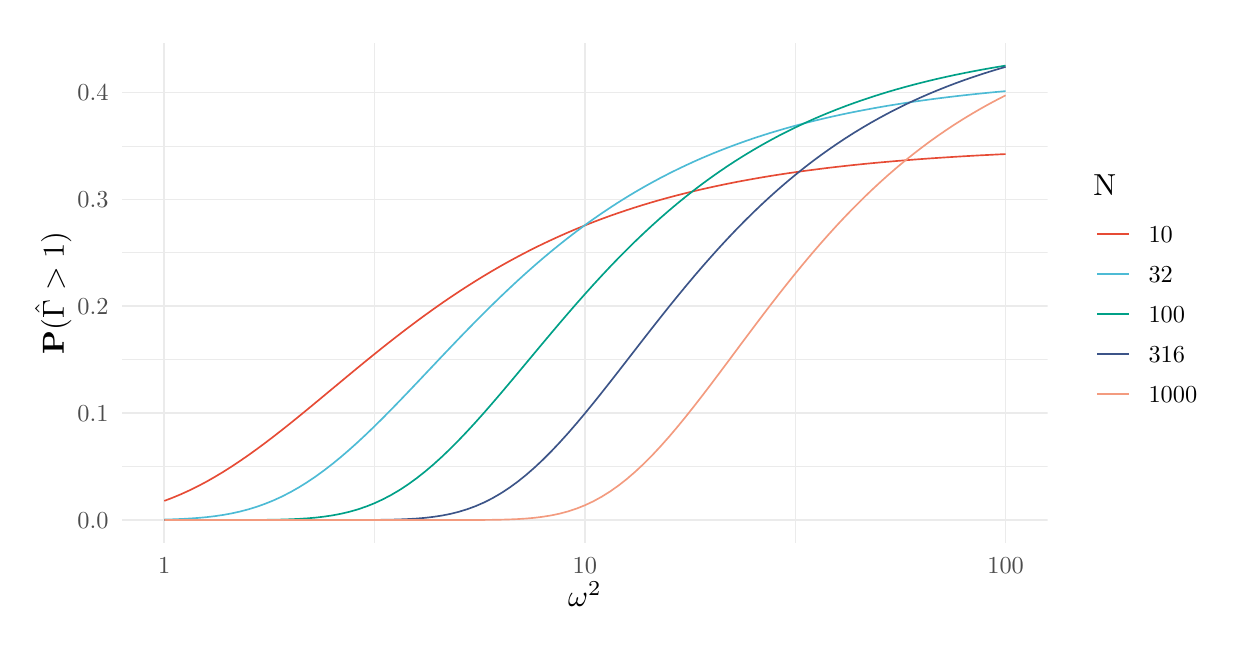
\begin{tikzpicture}[x=1pt,y=1pt]
\definecolor{fillColor}{RGB}{255,255,255}
\path[use as bounding box,fill=fillColor,fill opacity=0.00] (0,0) rectangle (433.62,216.81);
\begin{scope}
\path[clip] ( 34.16, 30.69) rectangle (368.57,211.31);
\definecolor{drawColor}{gray}{0.92}

\path[draw=drawColor,line width= 0.3pt,line join=round] ( 34.16, 58.20) --
	(368.57, 58.20);

\path[draw=drawColor,line width= 0.3pt,line join=round] ( 34.16, 96.82) --
	(368.57, 96.82);

\path[draw=drawColor,line width= 0.3pt,line join=round] ( 34.16,135.43) --
	(368.57,135.43);

\path[draw=drawColor,line width= 0.3pt,line join=round] ( 34.16,174.05) --
	(368.57,174.05);

\path[draw=drawColor,line width= 0.3pt,line join=round] (125.36, 30.69) --
	(125.36,211.31);

\path[draw=drawColor,line width= 0.3pt,line join=round] (277.37, 30.69) --
	(277.37,211.31);

\path[draw=drawColor,line width= 0.6pt,line join=round] ( 34.16, 38.90) --
	(368.57, 38.90);

\path[draw=drawColor,line width= 0.6pt,line join=round] ( 34.16, 77.51) --
	(368.57, 77.51);

\path[draw=drawColor,line width= 0.6pt,line join=round] ( 34.16,116.13) --
	(368.57,116.13);

\path[draw=drawColor,line width= 0.6pt,line join=round] ( 34.16,154.74) --
	(368.57,154.74);

\path[draw=drawColor,line width= 0.6pt,line join=round] ( 34.16,193.35) --
	(368.57,193.35);

\path[draw=drawColor,line width= 0.6pt,line join=round] ( 49.36, 30.69) --
	( 49.36,211.31);

\path[draw=drawColor,line width= 0.6pt,line join=round] (201.36, 30.69) --
	(201.36,211.31);

\path[draw=drawColor,line width= 0.6pt,line join=round] (353.37, 30.69) --
	(353.37,211.31);
\definecolor{drawColor}{RGB}{230,75,53}

\path[draw=drawColor,line width= 0.6pt,line join=round] ( 49.36, 45.81) --
	( 52.40, 46.97) --
	( 55.44, 48.24) --
	( 58.48, 49.62) --
	( 61.52, 51.12) --
	( 64.56, 52.73) --
	( 67.60, 54.46) --
	( 70.64, 56.28) --
	( 73.68, 58.21) --
	( 76.72, 60.23) --
	( 79.76, 62.33) --
	( 82.80, 64.52) --
	( 85.84, 66.77) --
	( 88.88, 69.09) --
	( 91.92, 71.46) --
	( 94.96, 73.88) --
	( 98.00, 76.34) --
	(101.04, 78.83) --
	(104.08, 81.34) --
	(107.12, 83.86) --
	(110.16, 86.39) --
	(113.20, 88.92) --
	(116.24, 91.44) --
	(119.28, 93.95) --
	(122.32, 96.44) --
	(125.36, 98.90) --
	(128.40,101.34) --
	(131.44,103.74) --
	(134.48,106.10) --
	(137.52,108.43) --
	(140.56,110.71) --
	(143.60,112.94) --
	(146.64,115.12) --
	(149.68,117.26) --
	(152.72,119.34) --
	(155.76,121.37) --
	(158.80,123.34) --
	(161.84,125.26) --
	(164.88,127.13) --
	(167.92,128.94) --
	(170.96,130.70) --
	(174.00,132.40) --
	(177.04,134.04) --
	(180.08,135.64) --
	(183.12,137.18) --
	(186.16,138.67) --
	(189.20,140.10) --
	(192.24,141.49) --
	(195.28,142.83) --
	(198.32,144.12) --
	(201.36,145.36) --
	(204.40,146.56) --
	(207.44,147.71) --
	(210.48,148.82) --
	(213.52,149.88) --
	(216.56,150.91) --
	(219.60,151.89) --
	(222.64,152.84) --
	(225.68,153.75) --
	(228.72,154.62) --
	(231.76,155.46) --
	(234.80,156.26) --
	(237.84,157.03) --
	(240.88,157.77) --
	(243.92,158.48) --
	(246.97,159.16) --
	(250.01,159.81) --
	(253.05,160.44) --
	(256.09,161.04) --
	(259.13,161.61) --
	(262.17,162.16) --
	(265.21,162.69) --
	(268.25,163.20) --
	(271.29,163.68) --
	(274.33,164.14) --
	(277.37,164.58) --
	(280.41,165.01) --
	(283.45,165.41) --
	(286.49,165.80) --
	(289.53,166.18) --
	(292.57,166.53) --
	(295.61,166.87) --
	(298.65,167.20) --
	(301.69,167.51) --
	(304.73,167.81) --
	(307.77,168.09) --
	(310.81,168.36) --
	(313.85,168.62) --
	(316.89,168.87) --
	(319.93,169.11) --
	(322.97,169.34) --
	(326.01,169.56) --
	(329.05,169.76) --
	(332.09,169.96) --
	(335.13,170.15) --
	(338.17,170.34) --
	(341.21,170.51) --
	(344.25,170.68) --
	(347.29,170.83) --
	(350.33,170.99) --
	(353.37,171.13);
\definecolor{drawColor}{RGB}{77,187,213}

\path[draw=drawColor,line width= 0.6pt,line join=round] ( 49.36, 39.07) --
	( 52.40, 39.15) --
	( 55.44, 39.27) --
	( 58.48, 39.44) --
	( 61.52, 39.65) --
	( 64.56, 39.93) --
	( 67.60, 40.29) --
	( 70.64, 40.74) --
	( 73.68, 41.29) --
	( 76.72, 41.96) --
	( 79.76, 42.76) --
	( 82.80, 43.69) --
	( 85.84, 44.78) --
	( 88.88, 46.01) --
	( 91.92, 47.41) --
	( 94.96, 48.97) --
	( 98.00, 50.70) --
	(101.04, 52.59) --
	(104.08, 54.64) --
	(107.12, 56.85) --
	(110.16, 59.20) --
	(113.20, 61.69) --
	(116.24, 64.31) --
	(119.28, 67.04) --
	(122.32, 69.88) --
	(125.36, 72.81) --
	(128.40, 75.82) --
	(131.44, 78.90) --
	(134.48, 82.03) --
	(137.52, 85.20) --
	(140.56, 88.39) --
	(143.60, 91.61) --
	(146.64, 94.82) --
	(149.68, 98.04) --
	(152.72,101.23) --
	(155.76,104.41) --
	(158.80,107.55) --
	(161.84,110.65) --
	(164.88,113.71) --
	(167.92,116.71) --
	(170.96,119.66) --
	(174.00,122.55) --
	(177.04,125.38) --
	(180.08,128.14) --
	(183.12,130.83) --
	(186.16,133.45) --
	(189.20,136.00) --
	(192.24,138.47) --
	(195.28,140.87) --
	(198.32,143.20) --
	(201.36,145.45) --
	(204.40,147.63) --
	(207.44,149.74) --
	(210.48,151.77) --
	(213.52,153.74) --
	(216.56,155.63) --
	(219.60,157.46) --
	(222.64,159.22) --
	(225.68,160.91) --
	(228.72,162.55) --
	(231.76,164.11) --
	(234.80,165.62) --
	(237.84,167.07) --
	(240.88,168.47) --
	(243.92,169.81) --
	(246.97,171.09) --
	(250.01,172.32) --
	(253.05,173.51) --
	(256.09,174.64) --
	(259.13,175.73) --
	(262.17,176.78) --
	(265.21,177.78) --
	(268.25,178.74) --
	(271.29,179.65) --
	(274.33,180.54) --
	(277.37,181.38) --
	(280.41,182.19) --
	(283.45,182.96) --
	(286.49,183.70) --
	(289.53,184.41) --
	(292.57,185.09) --
	(295.61,185.74) --
	(298.65,186.36) --
	(301.69,186.95) --
	(304.73,187.52) --
	(307.77,188.07) --
	(310.81,188.59) --
	(313.85,189.08) --
	(316.89,189.56) --
	(319.93,190.02) --
	(322.97,190.45) --
	(326.01,190.87) --
	(329.05,191.27) --
	(332.09,191.65) --
	(335.13,192.01) --
	(338.17,192.36) --
	(341.21,192.69) --
	(344.25,193.01) --
	(347.29,193.31) --
	(350.33,193.60) --
	(353.37,193.88);
\definecolor{drawColor}{RGB}{0,160,135}

\path[draw=drawColor,line width= 0.6pt,line join=round] ( 49.36, 38.90) --
	( 52.40, 38.90) --
	( 55.44, 38.90) --
	( 58.48, 38.90) --
	( 61.52, 38.90) --
	( 64.56, 38.90) --
	( 67.60, 38.90) --
	( 70.64, 38.90) --
	( 73.68, 38.90) --
	( 76.72, 38.91) --
	( 79.76, 38.92) --
	( 82.80, 38.93) --
	( 85.84, 38.96) --
	( 88.88, 39.00) --
	( 91.92, 39.07) --
	( 94.96, 39.17) --
	( 98.00, 39.31) --
	(101.04, 39.51) --
	(104.08, 39.77) --
	(107.12, 40.13) --
	(110.16, 40.58) --
	(113.20, 41.16) --
	(116.24, 41.87) --
	(119.28, 42.74) --
	(122.32, 43.77) --
	(125.36, 44.99) --
	(128.40, 46.40) --
	(131.44, 48.00) --
	(134.48, 49.80) --
	(137.52, 51.81) --
	(140.56, 54.01) --
	(143.60, 56.41) --
	(146.64, 58.99) --
	(149.68, 61.75) --
	(152.72, 64.66) --
	(155.76, 67.73) --
	(158.80, 70.92) --
	(161.84, 74.23) --
	(164.88, 77.63) --
	(167.92, 81.12) --
	(170.96, 84.67) --
	(174.00, 88.27) --
	(177.04, 91.90) --
	(180.08, 95.55) --
	(183.12, 99.20) --
	(186.16,102.84) --
	(189.20,106.46) --
	(192.24,110.05) --
	(195.28,113.60) --
	(198.32,117.10) --
	(201.36,120.53) --
	(204.40,123.91) --
	(207.44,127.21) --
	(210.48,130.45) --
	(213.52,133.60) --
	(216.56,136.67) --
	(219.60,139.66) --
	(222.64,142.56) --
	(225.68,145.38) --
	(228.72,148.11) --
	(231.76,150.75) --
	(234.80,153.31) --
	(237.84,155.78) --
	(240.88,158.17) --
	(243.92,160.47) --
	(246.97,162.69) --
	(250.01,164.83) --
	(253.05,166.89) --
	(256.09,168.87) --
	(259.13,170.77) --
	(262.17,172.60) --
	(265.21,174.36) --
	(268.25,176.05) --
	(271.29,177.68) --
	(274.33,179.24) --
	(277.37,180.73) --
	(280.41,182.16) --
	(283.45,183.54) --
	(286.49,184.86) --
	(289.53,186.12) --
	(292.57,187.33) --
	(295.61,188.49) --
	(298.65,189.60) --
	(301.69,190.66) --
	(304.73,191.68) --
	(307.77,192.65) --
	(310.81,193.59) --
	(313.85,194.48) --
	(316.89,195.33) --
	(319.93,196.15) --
	(322.97,196.93) --
	(326.01,197.68) --
	(329.05,198.40) --
	(332.09,199.08) --
	(335.13,199.74) --
	(338.17,200.36) --
	(341.21,200.96) --
	(344.25,201.53) --
	(347.29,202.08) --
	(350.33,202.60) --
	(353.37,203.10);
\definecolor{drawColor}{RGB}{60,84,136}

\path[draw=drawColor,line width= 0.6pt,line join=round] ( 49.36, 38.90) --
	( 52.40, 38.90) --
	( 55.44, 38.90) --
	( 58.48, 38.90) --
	( 61.52, 38.90) --
	( 64.56, 38.90) --
	( 67.60, 38.90) --
	( 70.64, 38.90) --
	( 73.68, 38.90) --
	( 76.72, 38.90) --
	( 79.76, 38.90) --
	( 82.80, 38.90) --
	( 85.84, 38.90) --
	( 88.88, 38.90) --
	( 91.92, 38.90) --
	( 94.96, 38.90) --
	( 98.00, 38.90) --
	(101.04, 38.90) --
	(104.08, 38.90) --
	(107.12, 38.90) --
	(110.16, 38.90) --
	(113.20, 38.90) --
	(116.24, 38.90) --
	(119.28, 38.91) --
	(122.32, 38.92) --
	(125.36, 38.94) --
	(128.40, 38.98) --
	(131.44, 39.03) --
	(134.48, 39.12) --
	(137.52, 39.25) --
	(140.56, 39.43) --
	(143.60, 39.69) --
	(146.64, 40.05) --
	(149.68, 40.51) --
	(152.72, 41.11) --
	(155.76, 41.87) --
	(158.80, 42.79) --
	(161.84, 43.91) --
	(164.88, 45.23) --
	(167.92, 46.77) --
	(170.96, 48.53) --
	(174.00, 50.52) --
	(177.04, 52.73) --
	(180.08, 55.17) --
	(183.12, 57.82) --
	(186.16, 60.67) --
	(189.20, 63.71) --
	(192.24, 66.93) --
	(195.28, 70.29) --
	(198.32, 73.80) --
	(201.36, 77.42) --
	(204.40, 81.14) --
	(207.44, 84.94) --
	(210.48, 88.79) --
	(213.52, 92.68) --
	(216.56, 96.60) --
	(219.60,100.52) --
	(222.64,104.44) --
	(225.68,108.33) --
	(228.72,112.18) --
	(231.76,116.00) --
	(234.80,119.75) --
	(237.84,123.44) --
	(240.88,127.06) --
	(243.92,130.60) --
	(246.97,134.06) --
	(250.01,137.44) --
	(253.05,140.72) --
	(256.09,143.91) --
	(259.13,147.01) --
	(262.17,150.01) --
	(265.21,152.92) --
	(268.25,155.73) --
	(271.29,158.45) --
	(274.33,161.07) --
	(277.37,163.60) --
	(280.41,166.04) --
	(283.45,168.39) --
	(286.49,170.65) --
	(289.53,172.82) --
	(292.57,174.91) --
	(295.61,176.92) --
	(298.65,178.85) --
	(301.69,180.70) --
	(304.73,182.48) --
	(307.77,184.18) --
	(310.81,185.82) --
	(313.85,187.39) --
	(316.89,188.89) --
	(319.93,190.33) --
	(322.97,191.71) --
	(326.01,193.03) --
	(329.05,194.29) --
	(332.09,195.50) --
	(335.13,196.66) --
	(338.17,197.77) --
	(341.21,198.83) --
	(344.25,199.85) --
	(347.29,200.82) --
	(350.33,201.75) --
	(353.37,202.64);
\definecolor{drawColor}{RGB}{243,155,127}

\path[draw=drawColor,line width= 0.6pt,line join=round] ( 49.36, 38.90) --
	( 52.40, 38.90) --
	( 55.44, 38.90) --
	( 58.48, 38.90) --
	( 61.52, 38.90) --
	( 64.56, 38.90) --
	( 67.60, 38.90) --
	( 70.64, 38.90) --
	( 73.68, 38.90) --
	( 76.72, 38.90) --
	( 79.76, 38.90) --
	( 82.80, 38.90) --
	( 85.84, 38.90) --
	( 88.88, 38.90) --
	( 91.92, 38.90) --
	( 94.96, 38.90) --
	( 98.00, 38.90) --
	(101.04, 38.90) --
	(104.08, 38.90) --
	(107.12, 38.90) --
	(110.16, 38.90) --
	(113.20, 38.90) --
	(116.24, 38.90) --
	(119.28, 38.90) --
	(122.32, 38.90) --
	(125.36, 38.90) --
	(128.40, 38.90) --
	(131.44, 38.90) --
	(134.48, 38.90) --
	(137.52, 38.90) --
	(140.56, 38.90) --
	(143.60, 38.90) --
	(146.64, 38.90) --
	(149.68, 38.90) --
	(152.72, 38.90) --
	(155.76, 38.90) --
	(158.80, 38.91) --
	(161.84, 38.92) --
	(164.88, 38.93) --
	(167.92, 38.97) --
	(170.96, 39.02) --
	(174.00, 39.11) --
	(177.04, 39.24) --
	(180.08, 39.43) --
	(183.12, 39.70) --
	(186.16, 40.08) --
	(189.20, 40.57) --
	(192.24, 41.21) --
	(195.28, 42.02) --
	(198.32, 43.02) --
	(201.36, 44.23) --
	(204.40, 45.66) --
	(207.44, 47.33) --
	(210.48, 49.23) --
	(213.52, 51.38) --
	(216.56, 53.77) --
	(219.60, 56.40) --
	(222.64, 59.24) --
	(225.68, 62.30) --
	(228.72, 65.56) --
	(231.76, 68.98) --
	(234.80, 72.57) --
	(237.84, 76.29) --
	(240.88, 80.12) --
	(243.92, 84.04) --
	(246.97, 88.03) --
	(250.01, 92.07) --
	(253.05, 96.14) --
	(256.09,100.23) --
	(259.13,104.31) --
	(262.17,108.36) --
	(265.21,112.39) --
	(268.25,116.37) --
	(271.29,120.30) --
	(274.33,124.15) --
	(277.37,127.94) --
	(280.41,131.64) --
	(283.45,135.26) --
	(286.49,138.78) --
	(289.53,142.21) --
	(292.57,145.55) --
	(295.61,148.78) --
	(298.65,151.91) --
	(301.69,154.95) --
	(304.73,157.88) --
	(307.77,160.71) --
	(310.81,163.45) --
	(313.85,166.08) --
	(316.89,168.62) --
	(319.93,171.06) --
	(322.97,173.42) --
	(326.01,175.68) --
	(329.05,177.85) --
	(332.09,179.93) --
	(335.13,181.94) --
	(338.17,183.86) --
	(341.21,185.70) --
	(344.25,187.47) --
	(347.29,189.17) --
	(350.33,190.79) --
	(353.37,192.35);
\end{scope}
\begin{scope}
\path[clip] (  0.00,  0.00) rectangle (433.62,216.81);
\definecolor{drawColor}{gray}{0.30}

\node[text=drawColor,anchor=base east,inner sep=0pt, outer sep=0pt, scale=  0.88] at ( 29.21, 35.87) {0.0};

\node[text=drawColor,anchor=base east,inner sep=0pt, outer sep=0pt, scale=  0.88] at ( 29.21, 74.48) {0.1};

\node[text=drawColor,anchor=base east,inner sep=0pt, outer sep=0pt, scale=  0.88] at ( 29.21,113.09) {0.2};

\node[text=drawColor,anchor=base east,inner sep=0pt, outer sep=0pt, scale=  0.88] at ( 29.21,151.71) {0.3};

\node[text=drawColor,anchor=base east,inner sep=0pt, outer sep=0pt, scale=  0.88] at ( 29.21,190.32) {0.4};
\end{scope}
\begin{scope}
\path[clip] (  0.00,  0.00) rectangle (433.62,216.81);
\definecolor{drawColor}{gray}{0.30}

\node[text=drawColor,anchor=base,inner sep=0pt, outer sep=0pt, scale=  0.88] at ( 49.36, 19.68) {1};

\node[text=drawColor,anchor=base,inner sep=0pt, outer sep=0pt, scale=  0.88] at (201.36, 19.68) {10};

\node[text=drawColor,anchor=base,inner sep=0pt, outer sep=0pt, scale=  0.88] at (353.37, 19.68) {100};
\end{scope}
\begin{scope}
\path[clip] (  0.00,  0.00) rectangle (433.62,216.81);
\definecolor{drawColor}{RGB}{0,0,0}

\node[text=drawColor,anchor=base,inner sep=0pt, outer sep=0pt, scale=  1.10] at (201.36,  7.64) {$\omega^2$};
\end{scope}
\begin{scope}
\path[clip] (  0.00,  0.00) rectangle (433.62,216.81);
\definecolor{drawColor}{RGB}{0,0,0}

\node[text=drawColor,rotate= 90.00,anchor=base,inner sep=0pt, outer sep=0pt, scale=  1.10] at ( 13.08,121.00) {$\mathbf P ( \hat \Gamma > 1 )$};
\end{scope}
\begin{scope}
\path[clip] (  0.00,  0.00) rectangle (433.62,216.81);
\definecolor{drawColor}{RGB}{0,0,0}

\node[text=drawColor,anchor=base west,inner sep=0pt, outer sep=0pt, scale=  1.10] at (385.07,156.09) {N};
\end{scope}
\begin{scope}
\path[clip] (  0.00,  0.00) rectangle (433.62,216.81);
\definecolor{drawColor}{RGB}{230,75,53}

\path[draw=drawColor,line width= 0.6pt,line join=round] (386.52,142.30) -- (398.08,142.30);
\end{scope}
\begin{scope}
\path[clip] (  0.00,  0.00) rectangle (433.62,216.81);
\definecolor{drawColor}{RGB}{77,187,213}

\path[draw=drawColor,line width= 0.6pt,line join=round] (386.52,127.84) -- (398.08,127.84);
\end{scope}
\begin{scope}
\path[clip] (  0.00,  0.00) rectangle (433.62,216.81);
\definecolor{drawColor}{RGB}{0,160,135}

\path[draw=drawColor,line width= 0.6pt,line join=round] (386.52,113.39) -- (398.08,113.39);
\end{scope}
\begin{scope}
\path[clip] (  0.00,  0.00) rectangle (433.62,216.81);
\definecolor{drawColor}{RGB}{60,84,136}

\path[draw=drawColor,line width= 0.6pt,line join=round] (386.52, 98.94) -- (398.08, 98.94);
\end{scope}
\begin{scope}
\path[clip] (  0.00,  0.00) rectangle (433.62,216.81);
\definecolor{drawColor}{RGB}{243,155,127}

\path[draw=drawColor,line width= 0.6pt,line join=round] (386.52, 84.48) -- (398.08, 84.48);
\end{scope}
\begin{scope}
\path[clip] (  0.00,  0.00) rectangle (433.62,216.81);
\definecolor{drawColor}{RGB}{0,0,0}

\node[text=drawColor,anchor=base west,inner sep=0pt, outer sep=0pt, scale=  0.88] at (405.02,139.27) {10};
\end{scope}
\begin{scope}
\path[clip] (  0.00,  0.00) rectangle (433.62,216.81);
\definecolor{drawColor}{RGB}{0,0,0}

\node[text=drawColor,anchor=base west,inner sep=0pt, outer sep=0pt, scale=  0.88] at (405.02,124.81) {32};
\end{scope}
\begin{scope}
\path[clip] (  0.00,  0.00) rectangle (433.62,216.81);
\definecolor{drawColor}{RGB}{0,0,0}

\node[text=drawColor,anchor=base west,inner sep=0pt, outer sep=0pt, scale=  0.88] at (405.02,110.36) {100};
\end{scope}
\begin{scope}
\path[clip] (  0.00,  0.00) rectangle (433.62,216.81);
\definecolor{drawColor}{RGB}{0,0,0}

\node[text=drawColor,anchor=base west,inner sep=0pt, outer sep=0pt, scale=  0.88] at (405.02, 95.91) {316};
\end{scope}
\begin{scope}
\path[clip] (  0.00,  0.00) rectangle (433.62,216.81);
\definecolor{drawColor}{RGB}{0,0,0}

\node[text=drawColor,anchor=base west,inner sep=0pt, outer sep=0pt, scale=  0.88] at (405.02, 81.45) {1000};
\end{scope}
\end{tikzpicture}
%
    }
    \caption{
        We show the probability that the estimated posterior variance $\hat \Gamma$ is bigger than the prior variance $1$ when varying the noise variance $\omega^{2}$. {\color{red} todo: ausführlicher beschreiben} %
        % for small N: N / N-1 difference in estimation
        % as omega grows, prob. increases
        % as N increases, larger omega necessary
    }
    \label{fig:ce_prob_failure}
\end{figure}

% all of these even worse if dimension grows
In higher-dimensional settings, e.g. when applying the \gls{cem} to \glspl{ssm}, we can expect this phenomenon to occur even more often. In the extreme case of independent marginals, i.e. when $\Sigma$ is a diagonal matrix, \Cref{eq:gamma_post} reduces to $(n + 1)p$ many decoupled equations, where $\hat \Gamma_{i,i}, i =1, \dots, (n + 1)p$ are independent. If all $q_{i} = \P \left(\Gamma_{i,i} > \Sigma_{i,i}\right)$ are identical to $q \in (0, 1)$, e.g. because $\Sigma$ and $\Omega$ are multiples of the identity, the number of failures follows a $\operatorname{Binom} \left( (n + 1)p, q \right)$ distribution, so that even small $q$ may lead to a non-negligible number of failures if the number of observations is high. 

% numerical scheme to solve eq.
Finally, in the multivariate setting, the system \eqref{eq:gamma_post} has no analytical solution. Instead, we have to resort to numerical methods to find a solution $\Omega$. Unfortunately, even evaluating the right-hand side of \eqref{eq:gamma_post} requires $\mathcal O(m^3)$ operations, as we have to invert $\Sigma + \Omega$. Additionally, we cannot hope to reuse a singular-value, LR, or eigenvalue-decomposition for further evaluations, as $\Sigma$ and $\Omega$ are not guaranteed to be jointly diagonalizable.
In the \gls{ssm} context we may use the Kalman-smoother to compute the marginal variances, but have to re-run the smoother for every evaluation. 

If we admit noise variance $\infty$ in the univariate setting, then $\Gamma > 1$ implies that the \gls{cem} chooses this as the estimate, i.e. $\G_{\hpce}$ is $\mathcal N(0, 1)$, which is equal to the prior. We can interpret this as having a missing observation, which, going back to the \gls{ssm} context, the Kalman-filter (\Cref{alg:kalman_filter}) can handle with only simple modifications, see e.g. \cite[Section 4.10]{Durbin2012Time}. However, if there are a lot of failures, the optimally chosen $\G_{\hpce}$ will be close to the prior distribution of states $X$, and importance sampling is unlikely to be effective. Hence, we turn to another approach that allows us to apply the \gls{cem} to \glspl{ssm}.

\subsection{The Markov-approach}
\label{subsec:markov-approach}
% second: Gaussian Markov process 
% discuss more flexible vs. fewer parameters
An alternative family of Gaussian proposals is given by directly modeling a Gaussian Markov process on the states $X_{:n}$. Again, this is sensible given the Markov structure of the target. This parametrization is more flexible than using the posterior of a \gls{glssm} with fixed prior as the proposal. This flexibility, however, comes at the cost of requiring a larger number of parameters. Here we propose with $\G_{\psi}$ where
\begin{align}
    \begin{split}
    \label{eq:markov-proposal}
    \G_{\psi} &= \mathcal L (U + v), \\
    v &\in \R^{(n + 1)m}, \\
    U_{0} &\sim \mathcal N(0, R_{0}R_{0}^T),\\
    U_{t} &= C_{t}U_{t - 1} + R_{t}\nu_{t}, \\
    C_{t} &\in \R^{m\times m},\\
    \nu_{t} &\sim \mathcal N(0,I), \\
    R_{t}&\in\R^{m \times m} \text{ lower triangular with positive diagonal}
    \end{split}
\end{align}
for $t = 1, \dots, n$, with $U_{0}$ and $\nu_{1}, \dots, \nu_{n}$ independent. The number of parameters in $$\psi= \left( v, C_{1}, \dots, C_{n}, R_{0}, \dots, R_{n} \right)$$ is $(n + 1)\cdot m$ for the mean $v$, $n \cdot m^{2}$ for the transition matrices $C_{t}$ and $(n + 1) \frac{m (m - 1)}{2}$ for the Cholesky roots of innovation covariances, totaling $\mathcal O(n\cdot m^{2})$ many parameters. 
While these are considerably more parameters than for the \gls{glssm}-approach for large state dimension $m$, we will see in the later part of this section that finding the optimal parameters for the \gls{cem} can be done analytically. 

This approach, which we term the \textbf{Markov-approach}, was originally proposed by \citeauthor{Richard2007Efficient} in \cite{Richard2007Efficient} for general unnormalized transition kernels as \gls{eis} proposals. However, because of its lower number of parameters, one should favor the \gls{glssm}-approach for \gls{eis} that operates on the signals, see \cite{Koopman2019Modified}.

To perform importance sampling with $\G_{\psi}$ in model \eqref{eq:markov-proposal} we not only need to simulate from $\G_{\psi}$ but also evaluate the unnormalized importance sampling weights $w(x) = \frac{p(x|y)}{g_{\psi}(x)}$. Simulation from $\G_{\psi}$ is achieved by a simple recursion. For the weights note that 
\begin{align}
\label{eq:weights_markov}
w(x) \propto \frac{p(y|x)p(x)}{g_{\psi}(x)} = \prod_{t = 0}^n \frac{p(y_{t}|x_{t})p(x_{t}|x_{t - 1})}{g_{\psi}(x_{t}|x_{t - 1})},
\end{align}
where $p(x_{0}|x_{-1}) = p(x_{0})$ and $g_{\psi}(x_{0}|x_{-1}) = g_{\psi}(x_{0})$.

The Markov structure of model \eqref{eq:markov-proposal} implies that the precision matrix of $\G_{\psi}$ is sparse, i.e. it has a block-tridiagonal form. This is a well-known property of the precision matrix of Gaussian random vectors, as the following two classical lemmas show. We show their proofs here for completeness. For a general treatment, we refer the reader to \cite[Chapters 3 and 5]{Lauritzen1996Graphical}.

\begin{lemma}
    \label{lem:gaussian_precision}
    Let $(X,Y)$ be jointly Gaussian with distribution $\mathcal N \left( \mu, \Sigma \right)$ where 
    $$
    \mu = \left(\mu_{X}, \mu_{Y}\right)
    $$
    and 
    $$
    \Sigma = \begin{pmatrix}
        \Sigma_{XX} & \Sigma_{XY} \\
        \Sigma_{YX} & \Sigma_{YY}
    \end{pmatrix},
    $$
    are partitioned according to the dimensions of $X$ and $Y$ and $\Sigma$ is non-singular.
    If $$P = \Sigma^{-1} = \begin{pmatrix} \Sigma_{XX} &  \Sigma_{XY} \\ \Sigma_{XY} & \Sigma_{YY} \end{pmatrix}^{-1}=  \begin{pmatrix} P_{XX} & P_{XY} \\ P_{YX} & P_{YY} \end{pmatrix}$$ 
    is the precision matrix of $(X,Y)$, partitioned as is $\Sigma$, then $\cov(X|Y) = P_{XX}^{-1}$.
\end{lemma}
\begin{proof}
    Without loss of generality, assume that both $X$ and $Y$ are centered. 
    The conditional density $p(x|y)$ is proportional (in $x$) to the joint density $p(x,y)$ with 
    $$\log p(x,y) = -\frac 1 2 \begin{pmatrix} x & y\end{pmatrix}  P \begin{pmatrix} x\\y\end{pmatrix} + C = -\frac 12 \left(x^TP_{XX}x + 2x^TP_{XY}y\right) + C',$$
    for constants $C, C'$ that do not depend on $x$. 
    As the conditional distribution of $X$ given $Y=y$ is Gaussian (by \Cref{lem:gaussian_conditional}), its covariance matrix is $P_{XX}^{-1}$.
\end{proof}

\begin{lemma}
    \label{lem:gaussian_precision_zeros}
    Let $(X,Y,Z) \sim \mathcal N \left( \mu, \Sigma \right)$ be jointly Gaussian with non-singular $\Sigma$. Then $X \perp Y | Z$ if, and only if, the sub-matrix of the precision matrix $P = \Sigma^{-1}$ whose rows correspond to the entries of $X$ and columns correspond to the entries of $Y$ is the $0$ matrix.
\end{lemma}
\begin{proof}
    Partition the conditional covariance matrix into
    $$
    \cov \left((X,Y) | Z\right) = \begin{pmatrix}
        \Sigma_{XX|Z} & \Sigma_{XY|Z} \\
        \Sigma_{YX|Z} & \Sigma_{YY|Z}
    \end{pmatrix}.
    $$

    Now as all distributions involved are Gaussian, $X \perp Y | Z$ is equivalent to $\cov \left( (X,Y) |Z \right)$ being a block-diagonal matrix with blocks $\Sigma_{XX|Z}$ and $\Sigma_{YY|Z}$, which is equivalent to its inverse being a block-diagonal matrix with blocks $\Sigma_{XX|Z}^{-1}$ and $\Sigma_{YY|Z}^{-1}$. Its inverse is, by \Cref{lem:gaussian_precision}, the sub-matrix of $P$ whose rows and columns correspond to $X$ and $Y$. 
\end{proof}

Applying \Cref{lem:gaussian_precision_zeros} to model \eqref{eq:markov-proposal}, we see that its precision matrix $P$ is sparse, i.e. it is a block-tri-diagonal matrix, as $U_{t} \perp U_{s} | U_{-t,-s}$ for $\lvert t - s\rvert > 1$ and $U_{-t,-s}$ being the vector of all $U_{0}, \dots, U_{n}$ except for $U_{t}, U_{s}$. Thus, the only entries of $P$ that are potentially non-zero are those whose row and column correspond to $(U_{t}, U_{t})$ for $t = 0, \dots, n$, $(U_{t}, U_{t - 1})$ and $(U_{t - 1}, U_{t})$ for $t=1, \dots, n$. 

% show Cholesky root of precision matrix is also sparse -> Katzfuss (or refs therein), Lauritzen, Bernstein?, same as Schäfer paper?
The sparsity of $P$ implies that $P = LL^{T}$ has a sparse Cholesky root $L$, which will make computations efficient. 
To see that $L$ is sparse, we apply the following Theorem, slightly adapted to our notation, from the theory of Gaussian-Markov-Random-fields (GMRF), i.e. Gaussian models whose dependency structure is given by a graph, with edges between nodes indicating non-zero entries in the precision matrix.
\begin{theorem}[{\cite[Theorem 12.14]{Gelfand2010Discrete}}] 
    \label{thm:gelfand_gmrf}
    Let $X = (X_{0}, \dots, X_{n}) \in \R^{(n + 1)m}$ be a GMRF wrt to the labeled graph $G$, with mean $\mu$ and symmetric positive-definite precision matrix $P$. Let $L$ be the Cholesky factor of $P$ and define for $0 \leq t < s \leq n$ the future of $t$ except $s$ as 
    $$
        F(t,s) = \{t + 1, \dots, s - 1, s+ 1, n\}.
    $$
    Then
    $$
        X_{t} \perp X_{s} | X_{F(t,s)} \Leftrightarrow L_{t,s} = 0.
    $$
\end{theorem}
In the preceding theorem $X_{F(t,s)}$ is the vector of all $X_{u}$ for $u\in F(t,s)$ and $L_{t,s} \in \R^{m\times m}$ is the sub-matrix of $L$  whose rows correspond to $X_{t}$ and columns to $X_{s}$. 
From \Cref{thm:gelfand_gmrf} we immediately obtain the following:

\begin{corollary}[sparsity of $L$ in model \eqref{eq:markov-proposal}]
    \label{cor:sparsity_L}
    Let $U \sim \G_{\psi}$ as in \Cref{eq:markov-proposal}, $P \succ 0$ be the precision matrix of $\overset{\leftarrow}{U} = \left( U_{n}, \dots, U_{0} \right)$ and $L$ be the Cholesky root of $P$. 
    Then $L$ is a lower-block-diagonal matrix, with at most $n\,m^{2} + (n + 1)\,m\frac{m - 1}{2}$ non-zero entries:
    
    \begin{align}
        \label{eq:L_structure}
    L = \begin{pmatrix}
        L_{n,n} & 0 & \cdots & \cdots & \cdots & 0 & 0 \\
        L_{n-1, n} & L_{n-1,n-1} & 0 & \cdots & \cdots & 0 & 0\\
        0 & L_{n-2,n-1} & L_{n-2,n-2} & 0 & \cdots & 0 & 0 \\
        \vdots & \ddots & \ddots  & \ddots & \ddots & 0 & 0 \\
        0 & 0& 0& \cdots& L_{1, 2}& L_{1, 1} & 0 \\
        0 & 0 & 0 & \cdots & 0 & L_{0, 1} & L_{0,0} 
    \end{pmatrix},
    \end{align}
    where $L_{t,t} \in \R^{m\times m}, t = 0, \dots, n$ are lower triangular matrices with positive diagonal entries and $L_{t-1,t}\in\R^{m \times m}, t = 1, \dots, n$ are square matrices.
\end{corollary}

From $L$ in \Cref{cor:sparsity_L} we obtain an iterative method of sampling from $\G_{\psi}$: If $v + U \sim \G_{\psi}$, then, as $\cov U = \left( L L^{T} \right)^{-1} = L^{-T}L^{-1}$, it holds that $L^{T}U \sim \mathcal N(0, I)$ follows a standard normal distribution. Thus to simulate from $\G_{\psi}$ we may solve
$$
L^{T}U = \overset{\leftarrow} Z
$$
where $\overset{\leftarrow}Z = \left( Z_{n}, \dots, Z_{0} \right) \sim \mathcal N(0, I)$. Using the structure available in $L$, we see that this is equivalent to first solving
$$
L_{0,0}^T U_{0} = Z_{0}
$$
and then recursively solving for $t = 1, \dots, n$
$$
L_{t,t}^T U_{t} + L_{t-1, }^{T} U_{t-1} = Z_{t - 1}.
$$
Rearranging terms, provided $L_{t,t}$ is non-singular, we end up with the Markov-process
\begin{align}
\label{eq:rev_time_u}
    U_{t} = L^{-T}_{t,t} L_{t-1, t }^T U_{t - 1} +L^{-T}_{t,t} Z_{t},
\end{align}
where $Z_{t}$ is, by construction, independent of $U_{t}$. Thus for model \eqref{eq:markov-proposal}, we obtain
\begin{align}
    \label{eq:parameters_markov_from_L}
    \begin{split}
    R_{t} &= L^{-T}_{t,t} \text{ for } t = 0, \dots, n,\\
    C_{t} &= L^{-T}_{t,t} L_{t-1, t }^T \text{ for } t =1, \dots, n.
    \end{split}
\end{align}
Here we see why we chose to use $\overset{\leftarrow}U$ in \Cref{cor:sparsity_L}: had we applied \Cref{thm:gelfand_gmrf} to $U$ directly yields a Markov process in reverse time.

% show how to estimate Cholesky root analytically -> Schäfer
We now turn our attention to applying the \gls{cem} to model \eqref{eq:markov-proposal}. Following a similar argument as in the discussion surrounding \Cref{eq:cem_reparametrization}, we see that it suffices to choose $P$, the precision matrix of $U$, such that it minimizes
\begin{align}
\label{eq:markov_ce_target}
\frac{1}{2} \operatorname{trace} \left( P \hat\Gamma \right) - \frac{1}{2}\log\det P
\end{align}
where $\hat\Gamma$ is the importance sampling estimate of the joint covariance matrix of all states $X$. This is equivalent to minimizing 
$$
\Dkl{\mathcal N(0,\hat\Gamma)}{\mathcal N(0, P^{-1})}.
$$
Here $P$ is restricted to precision matrices that may arise in model \eqref{eq:markov-proposal}, i.e., by \Cref{cor:sparsity_L}, $P = LL^{T}$ where $L$ possess structure as in \eqref{eq:L_structure}. 
At first glance, this problem seems more involved than solving \Cref{eq:gamma_post}: after all, the optimal $P$ depends on the whole covariance matrix $\hat\Gamma$. 
However, it turns out that the sparsity we enforce in $L$ allows us to compute analytically the optimal $\hat L$  that minimizes 
\Cref{eq:markov_ce_target}. Additionally, due to the Markov-structure of our proposal, $\hat L$ depends only on the block-tri-diagonal component of $\hat \Gamma$, i.e. only the covariances $\cov(X_{t}, X_{t-1})$ and $\cov (X_{0})$ are required. This is sensible - all information about the Markov transitions is encoded in these covariances if we assume that $X$ is a Gaussian Markov process.

To make this argument rigorous, let us apply the following result (stated in our notation).
\begin{theorem}[{\cite[Theorem 2.1]{Schafer2021Sparse}}]
    \label{thm:schafer_cholesky_analytical}
    Let $\Gamma$ be a positive-definite matrix of size $n\times n$. Given a lower-triangular sparsity set $S \subset \{1, \dots, n\}^{2}$, i.e. $i \geq j$ for all $(i,j) \in S$, let 
    $$
    \hat L = \argmin_{L \in \mathcal S} \Dkl{\mathcal N (0, \Gamma)}{\mathcal N \left( 0, (LL^{T})^{-1} \right)}
    $$
    be the Cholesky root of the closest Gaussian (wrt. the \gls{kld}) with sparsity $\mathcal S = \{A \in \R^{n \times n}: A_{i,j} \neq 0 \Rightarrow (i,j) \in S\}$. 

    Then the following holds:
    The nonzero entries of the $i$-th column of $\hat L$ are given by 
    
    \begin{align}
    \label{eq:schafer_gamma}
        L_{s_{i}, i} &= \frac{\Gamma_{s_{i}, s_{i}}^{-1} e_{1}}{\sqrt{e_{1}^{T}\Gamma_{s_{i}, s_{i}}^{-1} e_{1}}},
    \end{align}
    where $s_{i} = \{j : (i,j) \in S\}$, $\Gamma_{s_{i}, s_{i}}$ is the restriction of $\Gamma$ to the set of indices $s_{i}$ and $e_{1} \in\R^{\lvert s_{i}\rvert}$ is the first unit vector.
\end{theorem}
For the problem at hand, the sparsity pattern $\mathcal S $ is given by the non-zero entries of $L$ depicted in \Cref{eq:L_structure} and the matrices $\Gamma_{s_{i}, s_{i}}$ are sub-matrices of the covariances $\cov \left( \left(X_{t-1}, X_{t}\right) | Y\right)$, for $t = 1, \dots, n$ and $\cov \left( X_{0} | Y\right)$, i.e. we let $\Gamma = \cov \left(\overset{\leftarrow}X| Y\right)$ in \Cref{thm:schafer_cholesky_analytical}.

Let $l^{j}_{t}\in \R^{2m\times m}$ be the $j$-th column of 
$$
\begin{pmatrix}
    L_{t,t} \\
    L_{t - 1, t}
\end{pmatrix},
$$
where $j \in \{1, \dots, m\}$. 
As $L_{t,t}$ is lower triangular, the first $j - 1$ entries of $l^{j}_t$ are $0$. We obtain the remaining nonzero entries by computing
$$
\frac{\Gamma_{t,j}^{-1}e_{j}}{\sqrt{e_{j}^T\Gamma_{t,j}^{-1}e_{j}}},
$$
for $\Gamma_{t,j}\in \R^{(2m - (j - 1))\times (2m - (j - 1))}$ the joint covariance matrix of the last $ m - (j - 1)$ components of $X_{t}$ and all entries of $X_{t - 1}$, conditional on $Y = y$, and $e_{j} \in \R^{2m - (j - 1)}$ the first unit vector.

Putting everything together, we may apply the \gls{cem} to estimate $\psi$ in model \eqref{eq:markov-proposal} in the following way: Given importance samples $U^{1}, \dots, U^{N}$ for $\mathcal L (X| Y = y)$ and associated unnormalized weights $w^{1}, \dots, w^{N}$, we estimate $v$ by 
\begin{align}
\label{eq:hat_v}
\hat v = \frac{\sum_{i = 1}^N w^{i}X^{i}}{\sum_{i = 1}^N w^{i}}
\end{align}
and the empirical covariance matrices
\begin{align}
    \label{eq:empirical_covs}
    \widehat{\cov} \left( X_{t}, X_{t - 1} \right) &= \frac{\sum_{i = 1}^N w^{i}(X_{t:t-1}^{i} - \hat v_{t-1:t}) (X_{t:t-1}^{i} - \hat v_{t-1:t})^{T}}{\sum_{i = 1}^N w^{i}}\\
\widehat{\cov} \left( X_{0}\right) &= \frac{\sum_{i = 1}^N w^{i}(X_{0}^{i} - \hat v_{0}) (X_{0}^{i} - \hat v_{0})^{T}}{\sum_{i = 1}^N w^{i}}.
\end{align}
We then determine $\hat L$ from these covariance matrices using \Cref{thm:schafer_cholesky_analytical}. 
These steps are summarized in \Cref{alg:cem-markov-proposal}. 

\begin{tcolorbox}[title={WIP improve: order to $\mathcal O(m^{3})$}]
    We can implement this more efficiently: Given sequential covariances $\cov (X_{t}, X_{t - 1})$, there exists a Markov process with these covariances (Cholesky roots give $L_{t}$ and $R_{t}$). As the optimal MP only depends on these covariances, we can also minimize KL-divergence to this MP. The KL divergence is thus minimized for this MP. Calculation of $L_{t}$ and $R_{t}$ then only take $\mathcal O((2m)^{3}) = \mathcal O(m^{3})$ instead of the $\mathcal O(m^{3})$ procedure presented until now. 
\end{tcolorbox}
\begin{algorithm}
    \caption{The \gls{cem} for the Markov proposal \eqref{eq:markov-proposal}}
    \label{alg:cem-markov-proposal}
    \begin{algorithmic}[1]
        \Require \gls{lcssm} (\Cref{def:lcssm}), observations $Y$, initial estimate $\hat\psi^0 = \left( v^{0}, C^{0}, R^{0}\right)$, sample size $N$
        \State set $l = 0$
        \Repeat 
            \State\label{step:cem-simulate} sample $U^{1} + v^{l}, \dots, U^{N} + v^{l} \iid \G_{\hat\psi^{l}}$ with fixed seed \Comment{\Cref{eq:markov-proposal}} 
            \State\label{step:cem-weights} determine unnormalized weights $w^{1}, \dots, w^{N}$ \Comment{\Cref{eq:weights_markov}}
            \State\label{step:cem-est_v} estimate $\hat v^{l + 1}$ \Comment{\Cref{eq:hat_v}} 
            \State\label{step:cem-est_cov} estimate $\widehat{\cov} (U_{t}, U_{t-1}), t=1, \dots, n$, $\widehat\cov (U_{0})$ \Comment{\Cref{eq:empirical_covs}}
            \State\label{step:cem-L} determine $\hat L^{l + 1}$ \Comment{\Cref{thm:schafer_cholesky_analytical}}
            \State\label{step:cem-C_R} determine $C^{l + 1}$ and $R^{l + 1}$ from $\hat L^{l + 1}$ \Comment{\Cref{eq:parameters_markov_from_L}}
            \State\label{step:cem-est_phi} set $\hat\psi^{l + 1} = \left( \hat v^{l + 1}, C^{l + 1}, R^{l + 1}\right)$ 
            \State set $l = l + 1$
        \Until{$\hat\psi^{l}$ converged}
        \State \textbf{return} $\hpce = \hat \psi^{l}$
    \end{algorithmic}
\end{algorithm}

% initial value: could also use LA/EIS
To run \Cref{alg:cem-markov-proposal} we require an initial value for $\hat\psi^{0}$. If a suitable $\hat\psi^{0}$ is not available, we can obtain one from the \gls{la} by sampling $X^{1}, \dots, X^{N}$ from the \gls{la} and performing steps \ref{step:cem-est_v} to \ref{step:cem-est_phi} from the loop.
Alternatively, we could also directly base our initial value on the smoothing distribution of the \gls{glssm} that the \gls{la} is based on. The Kalman smoother (\Cref{alg:kalman_smoother}) provides us with the analytically available covariances $\cov \left( X_{t}, X_{t - 1} | Z = z \right)$ and the marginal covariance $\cov \left( X_{0} | Z = z \right)$ can be computed as well. 

% convergence: number of iterations, rel. change in psi
The convergence criteria in \Cref{alg:cem-markov-proposal} is similar to that used for \gls{eis}: we stop until the absolute or entry-wise relative difference of $\hat\psi^{l}$ and $\hat \psi^{l + 1}$ is smaller than a predetermined threshold, or a fixed number of iterations has passed. For the matrices involved, we use the Frobenius norm and the Euclidean distance for the mean $v$. 

In \Cref{step:cem-simulate} we use the standard praxis of \glspl{crn} to ensure numerical convergence. This is similar to \gls{eis} and the maximum likelihood estimates from \Cref{sec:maximum_likelihood_estimation}.

% runtime
We give an overview of the time and space complexities of each line in \Cref{alg:cem-markov-proposal} in \Cref{tab:cem-time-space-complexity}
The total time complexity of single iteration of \Cref{alg:cem-markov-proposal} is $\mathcal O \left( N\,n\,m^{2} + n\,m^{4}\right)$ and its space complexity is $\mathcal O \left( N\,n\,m + n\,m^{2}\right)$. Let us elaborate on the complexities of each step:
\begin{enumerate}
    \item[\Cref{step:cem-simulate}] Generate $N$ i.i.d. samples from model \eqref{eq:markov-proposal}, where each simulation requires $\mathcal O(n)$ matrix-vector multiplications of dimension $m$. 
    \item[\Cref{step:cem-weights}] To evaluate the weights, \Cref{eq:weights_markov}, we have to evaluate for every sample $\mathcal O(n)$-times the density of a $m$-variate Gaussian distribution, while this usually has time-complexity $\mathcal O(m^{3})$, we have access to the Cholesky root $R_{t}$, so this step has only time-complexity $\mathcal O(m^{2})$. In \Cref{eq:weights_markov} we also need to compute $p(y_{t}|x_{t})$ and $p(x_{t}|x_{t - 1})$. Assuming conditional independence of observations, $p(y_{t}|x_{t}) = \prod_{i = 1}^{m}p(y_{t}^i|(B_{t}x_{t})^{i})$, evaluating the first term requires only $\mathcal O(m^{2})$ operations. For the second term, if we allow pre-computation of the Cholesky roots of innovations off-line (in $\mathcal O(m^{3})$ time), this step reduces to $\mathcal O(m^{2})$ as well.  
    \item[\Cref{step:cem-est_v}] Calculating the weighted mean $\hat v \in\R^{(n+1)m}$, \Cref{eq:hat_v}, requires $\mathcal O(N\,n\,m)$ operations.
    \item[\Cref{step:cem-est_cov}] Calculating the weighted covariance matrices, \Cref{eq:empirical_covs}, requires $(n+1)$ times multiplying $N$ many $m\times 1$ with $1 \times m$ vectors. 
    \item[\Cref{step:cem-L}] To determine $L_{t,t}$ and $L_{t - 1, t}$ we have to solve $m$ times the linear systems of equations given in \Cref{eq:schafer_gamma}, where the dimension of the system is $2m,\dots, m + 1$. This requires $\mathcal O(m^{4})$ many operations, and we have to perform it for every one of the $n + 1$ time points. The result is $L$ with sparsity structure given by \Cref{eq:L_structure}, which has $\mathcal O (n m^{2})$ many non-zero entries.
    \item[\Cref{step:cem-C_R}] For each of the $\mathcal O(n)$ many $C_{t}$ and $R_{t}$ we have to invert a triangular matrix of dimension $m$. 
\end{enumerate}

\begin{table}
    \centering
    \begin{tabular}{lcc}
        \toprule
        step & time complexity & space complexity \\
        \midrule 
        simulation (\Cref{step:cem-simulate}) & $\mathcal O \left( N\,n\,m^{2}\right)$ & $\mathcal O \left( N\,n\,m \right)$\\
        weights (\Cref{step:cem-weights}) & $\mathcal O (N\,n\,m^{2})$ & $\mathcal O \left( N \right)$\\
        estimating $v$ (\Cref{step:cem-est_v}) & $\mathcal O (N\,n\,m)$ & $\mathcal O \left( n\,m \right)$\\
        estimating covariances (\Cref{step:cem-est_cov}) & $\mathcal O (N\,n\,m^{2})$ & $\mathcal O \left( n\,m \right)$\\
        determining $L$ (\Cref{step:cem-L}) & $\mathcal O (n\,m^{4})$ & $\mathcal O (n \,m^{2})$\\
        determining $C$ and $R$ (\Cref{step:cem-C_R}) & $\mathcal O (n\,m^{3})$ & $\mathcal O (n\,m^{2})$\\
        \bottomrule
    \end{tabular}
    \caption{Time and space complexities of individual steps in \Cref{alg:cem-markov-proposal}.}
    \label{tab:cem-time-space-complexity}
\end{table}

An efficient implementation of \Cref{alg:cem-markov-proposal} can improve on some of the other steps involved. There is no need to calculate the $C_{t}$ and $R_{t}$ matrices explicitly, instead we can calculate $C_{t}U_{t - 1}$ efficiently by solving the linear system $L^{T}_{t,t}\left(C_{t}U_{t - 1}\right) = L_{t - 1, t}^TU_{t - 1}t$ by back-substitution, as $L^{T}_{t,t}$ is an upper triangular matrix. Similarly, to compute $R_{t}Z_{t}$ we solve $L^{T}_{t,t}\left( R_{t} Z_{t}\right) = Z_{t}$ by back-substitution. However, the main bottleneck for the time-complexity of \Cref{alg:cem-markov-proposal} is determining $L$ with time complexity $\mathcal O (n\,m^{4})$, which we have not been able to improve upon. 

% if space complexity is problematic, can compute weights first with fixed seed and then iterate forwards
If the main bottleneck for space lies in the $\mathcal O(N\,n\,m)$ simulation part, we may reduce this by simulating twice from model \eqref{eq:markov-proposal} using \glspl{crn}, and only storing the samples for a single time step (dimension $\mathcal O (N\,m)$) in each simulation. In the first pass, we only calculate the weights, and in the second pass, we calculate $\hat v$ and the required covariance matrices. For this, we only need the $2N$ samples of dimension $m$ from time $t$ and $t + 1$, i.e. $\mathcal O(N\,m)$ space. This reduces the total space complexity to $\mathcal O(N\,m + n\,m^{2})$. 

We demonstrate these improvements in \Cref{alg:cem-markov-proposal-fast}. Additionally, we calculate the weights on the log scale for numerical stability.

\begin{algorithm}
    \begin{algorithmic}
        \Require \gls{lcssm} (\Cref{def:lcssm}), observations $Y$, initial estimate $\hat\psi^0 = \left( v^{0}, L^{0}\right)$, sample size $N$
        \State set $l = 0$
        \Repeat 
            \State simulate $Z^{1}_0, \dots, Z^{N}_0 \iid \mathcal N(0, I)$ 
            \State set $U^{i}_0 = (L^{l}_{0,0})^{-T}Z_{0}^{i}$ \Comment{backsubstitution}
            \State set $X_{0}^{i} = v^{l}_{0} + U^{i}_0$ 
            \State set $\log w^{i} = \log p(y_{0}|X_{0}^{i}) + \log p(X_{0}^i) + \frac{1}{2} \lVert Z^{i}_0\rVert^{2}$ \Comment{$\log g(X_{0}^{i}) = -\frac{1}{2}\lVert Z^{i}_{0}\rVert^{2}_2 + C$ }
            \State store current RNG state
            \For {$t \gets 1, \dots, n$}
                \State simulate $Z^{1}_t, \dots, Z^{N}_t \iid \mathcal N(0, I)$ 
                \State set $U^{i}_t = (L^{l}_{t,t})^{-T}(L_{t - 1, t}^{l})^{T}U^{i}_{t - 1} + (L^{l}_{t,t})^{-T}Z_{t}^{i}$ \Comment{backsubstitution}
                \State set $X_{t}^{i} = v^{l}_{t} + U^{i}_t$ 
                \State set $\log w^{i} = \log w^{i} + \log p(y_{t}|X_{t}^{i}) + \log p(X_{t}^i|X_{t - 1}^i) + \frac{1}{2} \lVert Z^{i}_t\rVert^{2}$ 
            \EndFor
            \State set $\log w^{i} = \log w^{i} - \max_{i = 1,\dots, N} \log w^{i}$ \Comment{ensure $\log w^{i} \leq 0$}
            \State set $w^{i} = \exp (\log w^{i})$
            \State set $W^{i} = \frac{w^{i}}{\sum_{i = 1}^N w^{i}}$ \Comment{auto-normalized weights}
            \State set $v^{l + 1}_0 = \sum_{i = 1}^{N}W^{i}X_{0}^i$
            \State restore RNG state
            \For {$t \gets 1, \dots, n$}
                \State simulate $Z^{1}_t, \dots, Z^{N}_t \iid \mathcal N(0, I)$ 
                \State set $U^{i}_t = (L^{l}_{t,t})^{-T}(L^{l}_{t - 1, t})^{T}U^{i}_{t - 1} + (L^{l}_{t,t})^{-T}Z_{t}^{i}$ \Comment{backsubstitution}
                \State set $X_{t}^{i} = v^{l}_{t} + U^{i}_t$ 
                \State set $v^{l + 1}_t = \sum_{i = 1}^{N} W^{i}X^{i}_t$
                \State set $\widehat\cov \left( X_{t - 1}, X_{t} \right) = \sum_{i = 1}^N W^{i} \left( X^{i}_{t-1:t} - v^{l}_{t-1:t} \right)\left( X^{i}_{t-1:t} - v^{l}_{t-1:t} \right)^{T}$
            \EndFor
            \State determine $\hat L^{l + 1}$ \Comment{\Cref{thm:schafer_cholesky_analytical}}
            \State set $\hat\psi^{l + 1} = \left( \hat v^{l + 1}, \hat L^{l + 1}\right)$ 
            \State set $l = l + 1$
        \Until{$\hat\psi^{l}$ converged}
        \State \textbf{return} $\hpce = \hat \psi^{l}$
        
    \end{algorithmic}
    \caption{Time and space improved version of \Cref{alg:cem-markov-proposal}. Instructions involving the free index $i$ are to be performed for all $i = 1, \dots, N$ samples.}
    \label{alg:cem-markov-proposal-fast}
\end{algorithm}

The advantage of \Cref{alg:cem-markov-proposal,alg:cem-markov-proposal-fast} over applying the \gls{cem} to the \gls{glssm} model \eqref{eq:glssm-proposal} are multiple: First of all, as long as the involved covariance matrices are positive definite, the two algorithms produce valid proposals, i.e. they do not have the degeneracy problem we observed in \Cref{subsec:glssm-approach}.
% no numerical issues w/ determining optimal parameters
Additionally, determining the optimal parameters $(v,C,R)$ or $(v,L)$ is numerically stable, involving only inversion of small matrices. Compare this with solving \Cref{eq:gamma_post}, where we need to employ a numerical scheme to solve for the diagonal entries of $\Omega$.

% sampling faster 
After having determined $\hpce$ for model \eqref{eq:markov-proposal}, generating $N$ samples requires only $\mathcal O(N\,n\,m^{2})$ operations, whereas sampling from model \eqref{eq:glssm-proposal} requires $\mathcal O(n\,m^{3} + N\,n\,m^{2})$ operations, as we need an initial run of the Kalman filter. Unless $N < m$, this difference is negligible, and the case where $N < m$ is not really of interest, as we would expect importance sampling to require at least as many samples as there are dimensions, i.e. $N \gg m$. 

% problems: large state dimension: both $L$ and number of parameters
However, the two algorithms presented in this section also come with some drawbacks, especially if the dimension $m$ of states is large. This affects the algorithms in multiple ways: when $m$ is large, computation of $L$ becomes more time-intensive. Additionally, the dimension of the parameter $\psi$ increases quadratically in $m$, so we expect convergence to be slower, requiring a larger sample size $N$ to find the optimal $\hpce$. For an empirical study in this direction, see \Cref{sec:simulation_studies}.

% potential solution: directly estimate C + R?
To improve the speed of computation of both algorithms, $L$ has to be computed faster. 

\section{Accouting for multimodality and heavy tails}
%\label{sec:accouting_for_multimodality_and_heavy_tails}
%Performing importance sampling with the Gaussian models discussed so far will work well only if the smoothing distribution  $p(x|y)$ is well approximated by a Gaussian distribution. However, a Gaussian distribution is a very specific kind of distribution, in particular, it is an unimodal distribution
%%that is constant on elliptical contours 
%and has light tails \todo{check for correct wording}.
%
%If the smoothing distribution violates any of these assumptions, importance sampling with the models presented so far is likely to fail, i.e. requiring large sample sizes for both finding the optimal importance sampling parameter $\hat \psi$ as well as the final importance sampling evaluation.
%
%There are however techniques to keep most of the computational efficiency discussed in the above sections to address both multimodality as well as heavy tails.
%
%We start with heavier than gaussian tails: the textbook example of a heavy tailed distribution is the multivariate $t$-distribution with density
%$$
%    \dots .
%$$
%for degrees of freedom  $\nu > 1$ \todo{?}, location $\mu$ and scale matrix $\Sigma$. When $\nu > 2$ then this distribution has mean $\mu$ and if $\nu > 3$ it has covariance matrix $?$ \todo{check}.
%
%The main properties necessary to facilitate Gaussian importance sampling strategies above are that the distribution $p(x|y)$ is analytically tractable and simulation from it is possible. These properties still hold for the multivariate $t$-distribution and, in fact, for the even larger class of elliptical distributions:
%
%\begin{theorem}[Conditional distribution of elliptical distributions]
%    \label{thm:elliptical-conditional}
%    \todo{cite the correct book}
%\end{theorem}
%
%As one can readily see from \Cref{thm:elliptical-conditional} the parameters of the smoothing distribution $p(x|y)$ if $p(x,y)$ follows an elliptical distribution is again elliptical and its parameters only depend on quantities that are computed by the Kalman smoother. \todo{elaborate}
%
%\todo{present some models with heavy tails}
%
%
\section{Maximum likelihood estimation in SSMs}
\label{sec:maximum_likelihood_estimation}

% region introduction
%% need for MLE: hyperparameters
Until now, we have assumed that the \acrshort{ssm} under consideration is completely known, i.e. we have access to the true transition and observation kernels. For the models considered in this thesis (\Cref{cha:analysis_of_selected_models}), this is unrealistic, as they are not based on concrete physical processes but are rather statistical approximations of the true underlying dynamics. The transition densities of, e.g., \Cref{eq:glssm_states} will depend on the covariance matrix of innovations, of which we have no a priori knowledge and for negative binomially distributed observations the overdispersion parameter $r$ will be unknown. Let us denote by $\theta\in\R^{l}$ the vector of these hyperparameters. \todo{check l / k with psis}
To make this dependence explicit, we will introduce subscripts $\theta$ where appropriate, i.e. $\P_{\theta}$ is a target distribution that additionally depends on $\theta$, $p_{\theta}$ its density et cetera. This section is loosely based on \citep[Chapter 7 \& 11]{Durbin2012Time} and \citep[Chapter 14]{Chopin2020Introduction}

To determine a suitable value of $\theta$, multiple options are available. Here, we opt for a frequentist approach, using maximum likelihood estimation to determine an optimal $\hat \theta$. Therefore, given observations $y\in\R^{(n+1)\times p}$, $\hat\theta$ maximizes the likelihood $p_{\theta}(y)$ and can be obtained as the global maximum of the following optimization problem: 
$$
    \max_{\theta \in \Theta} p_{\theta}(y).
$$
For numerical stability, we should maximize the log-likelihood instead, i.e. solve 
\begin{align}
    \label{eq:max-log-p}
    \max_{\theta \in \Theta} \log p_{\theta}(y).
\end{align}
Here $\Theta \subseteq \R^{k}$ \todo{check k / l} is a space of feasible parameters. To solve this optimization problem using gradient ascent algorithms, we need access to both the likelihood and its derivatives. Thus, in the following, we will assume that $\theta \mapsto \log p_{\theta}(y)$ is sufficiently smooth, to apply these methods, i.e. it has continuous derivatives of second order. 

%% GLSSM analytically available, still need to use gradient descent algs. 
%% analytically impossible
%% high dimensional integral -> importance sampling
While the Kalman-filter (\Cref{alg:kalman_filter}) allows analytical computation of this likelihood \acrshortpl{glssm}, in general \acrshortpl{ssm} it is numerically intractable. The reason for this is that
$$
    p_{\theta}(y) = \int p_{\theta}(x,y) \mathrm d \mu(x)
$$
is a high-dimensional integral, which is hard to evaluate numerically. Instead, we will use importance sampling to estimate the likelihood. For this, let us regard $p_{\theta}(x,y)$ as an unnormalized density in $x$. The missing integration constant is then just $p_{\theta}(y)$ and the normalized density is $p_{\theta}(x|y)$. If $\G \gg \P$ is a proposal distribution whose density $g$ with respect to $\mu$ we can evaluate analytically, i.e. not only up to a constant, we see that for the unnormalized weights $\tilde w_{\theta}(x) = \frac{p_{\theta}(x,y)}{g(x)}$, that $p_{\theta}(y) = \G [\tilde w_{\theta}]$. Thus we may estimate the likelihood by 
$$
    \verywidehat{p_{\theta}(y)} = \frac{1}{N}\sum_{i = 1}^N \tilde w_{\theta} (X^{i})
$$
for $X^{1}, \dots, X^{N} \iid \G$ and $N \in \N$. To evaluate the gradient, notice that as $\nabla_{\theta} p_{\theta}(x,y) = p_{\theta}(x,y) \nabla_{\theta} \log p_{\theta}(x,y)$, we have, provided we can exchange integration and differentiation,
\begin{align*}
     \nabla_{\theta} p_{\theta}(y) &= \nabla_{\theta}\int p_{\theta}(x,y)\d \mu(x) = \int p_{\theta}(x,y) \nabla_{\theta} \log p_{\theta}(x,y)\d \mu(x) \\
     &= \G [\tilde w_{\theta} \nabla_{\theta} \log p_{\theta}(x,y)],
\end{align*}
and so we may estimate the gradient by 
\begin{align*}
    \verywidehat{\nabla_{\theta} p_{\theta}(y)} &= \frac{1}{N}\sum_{i = 1}^N \tilde w_{\theta}(X^{i}) \nabla_{\theta} \log p_{\theta}(X^{i}, y)
    %&= \sum_{i = 1}^N \tilde w_{\theta}(X^{i}) \sum_{t = 0}^n \nabla_{\theta} \left( \log p_{\theta}(y_{t} | X^{i}_{t}) + \log p_{\theta}(X^{i}_t|X^{i}_{t - 1}) \right).
\end{align*}
Similarly, we can estimate the log-likelihood by Plug-In
\begin{align}
    \label{eq:loglik-hat-standard}
    \verywidehat{\log p_{\theta}(y)} = \log \left( \frac{1}{N}\sum_{i = 1}^N \tilde w_{\theta}(X^{i}) \right)
\end{align}
and its gradient, using the fact that the gradient of $\log f$ for $f: \R^{l} \to \R$ is $ \frac{1}{f} \nabla_{\theta} f$, by 
\begin{align*}
    \verywidehat{\nabla_{\theta} \log p_{\theta}(y)} &= \left(\frac{1}{N} \sum_{i = 1}^N \tilde w_{\theta}(X^{i}) \right)^{-1} \left( \frac{1}{N}\sum_{i = 1}^N \tilde w_{\theta}(X^{i}) \nabla_{\theta} \log p_{\theta}(X^{i}, y) \right) \\
    &=\sum_{i = 1}^N W_{\theta}^{i} \nabla_{\theta} \log p_{\theta}(X^{i}, y)
\end{align*}
where $W_{\theta}^{i} = \frac{\tilde w_{\theta}(X^{i})}{\sum_{i= 1}^N \tilde w_{\theta}(X^{i})}$ are the auto-normalized weights.
Note that, by Jensen's inequality, these estimates are biased.


%% optimizatino using CRNs, advantage over particle filters
To solve the optimization problem \eqref{eq:max-log-p} we will again employ \acrshortpl{crn}. If the densities involved are twice differentiable, this device ensures that the random objective function $\theta \mapsto \sum_{i = 1}^N \tilde w_{\theta}(X^{i})$ is twice differentiable, and so we can indeed apply gradient ascent to find a local maximum. This is an advantage of performing global importance sampling over \acrshort{smc}, i.e. particle filter, methods. To avoid collapse to a single particle, \acrshort{smc} methods perform intermediate resampling steps, which make the objective function discontinuous. While particle smoothing methods can mitigate this problem, they are more expensive than standard \acrshort{smc} and, as the importance sampling estimates of the log-likelihood and its gradient are biased, the usual requirements for stochastic approximation methods are not fulfilled. 
For a more thorough discussion of the challenges maximum likelihood estimation with \acrshort{smc} methods faces, we recommend \citep[Chapter 14]{Chopin2020Introduction}.

%% discuss not really frequentist setting
While \acrshortpl{mle} have a strong frequentist foundation, let us stress that, for the models that we investigate in \Cref{cha:analysis_of_selected_models}, the frequentist properties of the estimates are not of interest. The reason for this is that a frequentist interpretation requires us to imagine, at least hypothetically, an infinite repetition of the data-generating process. For the data at hand, such repetition is nonsensical: the pandemic is a \glqq{}one-off\grqq{} event that will not be replicated under even approximately similar circumstances. Therefore, we will choose to view the estimation procedure more as a hyper-parameter tuning step, rather than true frequentist inference. While we can compute asymptotic confidence intervals for $\hat\theta$, see, e.g., \citep[Chapter 11.6]{Durbin2012Time}, \citep[Chapter 14.8]{Chopin2020Introduction}, these are not of practical interest for similar reasons. 

%% alternative: fully Bayesian
As an alternative to modeling $\theta$ as fixed, but unknown, and performing maximum-likelihood estimation to obtain $\hat \theta$, one might also model $\theta$ as random with prior density $p(\theta)$, such that the full model becomes $p(x,y,\theta) = p(x,y|\theta)p(\theta)$. In this setup, sometimes called the Bayesian treatment of \acrshortpl{ssm} \citep[Section 13.1]{Durbin2012Time}, the main interest still lies in the posterior density $p(x,\theta|y)$, which, depending on the model at hand, can drastically increase the difficulty of the problem: even if $p(x,y|\theta)$ is an analytically tractable model such as a \acrshort{glssm}, unless the prior is chosen to be conjugate, one has to resort to, e.g., \acrshort{mcmc}-methods. 

% endregion

% region GLSSM proposal

%% joint density easy to calculate
By the structure of the model, \Cref{eq:joint_density}, the log density and its gradient can be computed efficiently by
\begin{align*}
    \log p_{\theta}(x,y) &= \log p_{\theta}(x_{0}) + \sum_{t = 1}^{n} \log p_{\theta}(x_{t}|x_{t-1}) + \log p_{\theta} (y_{t}|x_{t},y_{t - 1})\\
    \nabla_{\theta}\log p_{\theta}(x,y) &= \nabla_{\theta}\log p_{\theta}(x_{0}) + \sum_{t = 1}^{n} \nabla_{\theta}\log p_{\theta}(x_{t}|x_{t-1}) + \nabla_{\theta}\log p_{\theta} (y_{t}|x_{t},y_{t - 1}),
\end{align*}
respectively. 

Similarly, when proposing with a \acrshort{glssm} or Markov-proposal for a \acrshort{pgssm}, the weights have similar structure, see\Cref{eq:weights_markov,eq:weights_only_on_signal}, which makes calculation of $\tilde w$ efficient. 

Considering the \acrshort{glssm}-proposal for a \acrshort{pgssm} with linear signal, we obtain 
$$
    \tilde w_{\theta}(x) = g(z)\frac{p_{\theta}(y|s)}{g(z|s)} = g(z) \prod_{t = 0}^n \frac{p_{\theta}(y_{t}|s_{t})}{g(z_{t}|s_{t})},
$$
where $s_{t} = B_{t}x_{t}$ is the signal, and so the estimated log-likelihood can evaluated efficiently as 
\begin{align}
    \label{eq:loglik-hat-linearsignal}
    \verywidehat{\log p_{\theta}(y)} = \log g_{\theta}(z) + \log \left(\frac{1}{N}\sum_{i=1}^{N}\prod_{t = 0}^{n} \frac{p_{\theta}(y_{t}|S^{i}_{t})}{ g(z_{t}|S^{i}_{t})}\right)
\end{align}
Notice that $\log g_{\theta}(z)$ is the likelihood in a \acrshort{glssm}, which can be computed efficiently by the standard Kalman filter (\Cref{alg:kalman_filter}). As in the \acrshort{glssm}-approach we propose with an \acrshort{glssm} whose state density $g(x)$ and observation matrices $B_{t}$, $t = 0, \dots, n$ are equal to those of the target, the log-likelihood $\log g_{\theta}(z)$ also depends on $\theta$. The estimated gradient of the log-likelihood is 
$$
    \verywidehat{\nabla_{\theta} \log p_{\theta}(y)} = \nabla_{\theta} \log g_{\theta}(z) + \sum_{i=1}^N W^{i}_\theta \sum_{t = 0}^n \nabla_{\theta} \log p_{\theta}(y_{t}|S_{t}^{i}).
$$
The gradient of the \acrshort{glssm} log-likelihood can be obtained either numerically or analytically by employing the Kalman filter and smoother \citep{Koopman1992Exact}, however, numerical evaluation may be faster if the dimension of $\theta$ is small compared to the length of the time series, as evaluating the likelihood only requires a single application of the Kalman filter. 

As the observation densities $g(z_{t}|s_{t})$ do not depend on $\theta$, their derivatives do not appear in the above estimate. However, when using the \acrshort{la} or \acrshort{eis} to determine an optimal proposal, the parameter $\psi = (z, \omega)$ implicitly depends on $\theta$. Accounting for this yields the gradient 
$$
    \verywidehat{\nabla_{\theta} \log p_{\theta}(y)} = \nabla_{\theta} \log g_{\theta}(z) + \sum_{i=1}^N W^{i}_\theta \left(\sum_{t = 0}^n \nabla_{\theta} \log p_{\theta}(y_{t}|S_{t}^{i}) - \nabla_{\theta} \log g_{\theta}(z_{t}|S^{i}_{t})\right),
$$
as $\nabla_{\theta} \frac{1}{g_{\theta}(z|s)} = - \frac{1}{g_{\theta}(z|s)} \nabla_{\theta} \log g_{\theta}(z|s)$. The computation of this additional term is much more involved, as the parameters $z,\Omega$ are found through an iterative numerical scheme. Instead, we favor numerical differentiation of the whole procedure to evaluate the likelihood at $\theta$, including the method of finding an optimal importance sampling scheme. 

\begin{algorithm}
    \begin{algorithmic}[1]
        \Require density $p_{\theta}$ of a parameterized \acrshort{pgssm}, $\theta \in \Theta$, observations $y \in \R^{(n+1)p}$
        \State determine importance sampling proposal $\G_{\psi(\theta)}$ \Comment{\Cref{alg:la}, \Cref{alg:eis} or \Cref{alg:cem-basic}}
        \State sample $X^{1}, \dots, X^{N} \iid \G_{\psi(\theta)}$
        \State compute $\widehat{\log p_{\theta}(y)}$ \Comment{\Cref{eq:loglik-hat-standard} or \Cref{eq:loglik-hat-linearsignal}}
        \State \textbf{return} $\widehat{\log p_{\theta}(y)}$
    \end{algorithmic}
    \caption{Estimation of log-likelihood $\verywidehat{\log p_{\theta}(y)}$}
\end{algorithm}

As a single evaluation of the log-likelihood can become very expensive we want our procedure to be as efficient as possible. To this end, \citep{Durbin1997Monte} provides several improvements to the basic algorithm if the model is a \acrshort{pgssm} with a linear signal. Their contributions consist of a bias correction for the log-likelihood, the use of antithetic and control variables to reduce Monte-Carlo error for importance sampling and a deterministic initialization procedure.
Let us briefly summarize these ideas, adapted to our notation. As the computational gains for control variates in the presence of antithetic variables seem to be limited, we do not give the same level of detail here, for an in-depth analysis, we refer the reader to the source. 

% bias reduction
For bias reduction, a second-order Taylor series expansion shows that for $\tilde{w}_\cdot = \frac{1}{N} \sum_{i =1}^N \tilde w(X^{i})$,
\begin{align*}
    \E \left(\log \tilde{w}_\cdot\right) - \log \G \tilde w &= \E \log \left(1 + \frac{\tilde{w}_\cdot - \G \tilde w}{\G \tilde w} \right)\\
                                                           &=  \frac{\tilde{w}_\cdot - \G \tilde w}{\G \tilde w}  - \frac{1}{2} \left(\frac{\tilde{w}_\cdot - \G \tilde w}{\G \tilde w} \right)^{2} + \mathcal O_{p}(N^{-\frac{3}{2}}),
\end{align*}
provided $\tilde w \in L^{3}(\G)$. Thus, estimating the second order term by $- \frac{\hat\sigma^2}{2N \tilde{w}_\cdot} $, where $\hat \sigma^{2}$ is the empirical variance of the unnormalized weights, we can perform a bias reduction by estimating 
\begin{align}
    \label{eq:loglik-hat-bias-reduction}
    \widehat{\log p_{\theta}(y)} = \log \left(\tilde w_{\cdot}\right) + \log g_{\theta}(z) + \frac{\hat\sigma^{2}}{2N\tilde w_{\cdot}}
\end{align}

% antithetics
The second improvement of \citep{Durbin1997Monte} is the use of antithetic variables and control variates, a device to reduce Monte-Carlo variance. The main idea of an antithetic variable is to construct for each sample $X^{i}$, $i = 1,\dots, N$, another sample $\tilde X^{i}$ that has the same distribution as $X^{i}$, but is negatively correlated with $X^{i}$. This has two effects: first of all, we increase the number of samples used for importance sampling and second, as the new samples are negatively correlated with the old samples, the Monte-Carlo variance is reduced. The computation of these samples is usually much faster than creating new samples, which requires the use of the expensive \acrshort{ffbs} or simulation smoother algorithms. 
\begin{definition}[antithetic variable]
    Let $X, \tilde X\in\R^{k}$ be two random variables with the same distribution, $\mathcal L (X) = \mathcal L(\tilde X)$ and $f: \R^{k} \to \R$. Then $\tilde X$ is called an antithetic variable of $X$ for $f$, if $\cov \left( f(\tilde X), f(X) \right) < 0$.
\end{definition}

% location & scale
\citep{Durbin1997Monte} introduce two antithetic variables: balanced for location and balanced for scale, both of which are tailored to the multivariate normal distribution. 
\begin{definition}[antithetic variable balanced for location and scale, \citep{Durbin1997Monte}]
    Let $X\sim \mathcal N(\mu, \Sigma)$ for $\mu \in \R^{k}$ and $\Sigma \in \R^{k\times k}$ positive definite. We call
    $$
    \tilde X = \mu + (\mu - X)
    $$
    the antithetic balanced for location. If $L\in\R^{k\times k}$ is a Cholesky root of $\Sigma$ and 
    $$
        X = \mu + L \varepsilon
    $$
    with $\varepsilon \sim \mathcal N(0, I)$, let $c = \varepsilon^{T}\varepsilon \sim \chi^{2}_k$ and $c' = F^{-1}_{\chi_{k}}(1 - F_{\chi_n}(\sqrt{c}))$\footnote{Note that unlike \citep{Durbin1997Monte} we use the $\chi_{k}$-distribution instead of their $\chi^{2}_k$ distribution, which makes the following proof somewhat simpler}. We call
    $$
        \check X = \mu + \sqrt{\frac{c'}{c}} \left( X - \mu \right)
    $$
    the antithetic balanced for location.
\end{definition}
\begin{lemma}
    Both $\tilde X$ and $\check X$ in the preceding lemma are antithetic variables for the coordinate functions $f_{i}:\R^{k} \to \R$, $f_{i}(x) = x_{i}$, $i = 1, \dots, k$.
\end{lemma}
\begin{proof}
    It is easy to see that $\tilde X$ has the same distribution as $X$. Furthermore 
    $$
        \cov \left( f_{i}(X), f_{i}(\tilde X)\right) = \cov \left( 2 \mu_{i} - X_{i}, X_{i} \right) = - \Sigma_{i,i} < 0.
    $$

    By the properties of the standard multivariate normal distribution, $ \lVert u \rVert $ and $ \frac{u}{ \lVert u \rVert }$ are independent. Writing 
    $$
        X = \mu + \lVert u \rVert L \frac{u}{ \lVert u \rVert } = \mu + \lVert u \rVert \frac{X - \mu}{\sqrt{c}},
    $$
    we see that 
    $$
        \check X = \mu + \sqrt{c'}\frac{X - \mu}{\sqrt{c}}
    $$
    has the same distribution as $X$, as $c' \sim \mathcal L( \lVert u \rVert^{2})$ and is independent of $ \frac{X - \mu}{\sqrt{c}}$. 
    Let $Z = \frac{X - \mu}{\sqrt{c}}$. Then $Z$ is centered and independent of both $c$, $c'$ and their product $cc'$. Thus 
    \begin{align*}
        \cov \left(f_{i}(X), f_{i}(\check X) \right) &= \cov \left( \sqrt{c} Z_{i}, \sqrt{c'}Z_{i} \right) = \E  \sqrt{cc'}Z_{i}^2 - \left( \E \sqrt c Z_{i} \right) \left( \E \sqrt {c'} Z_{i} \right) \\
        &= \E \sqrt{cc'} \E Z_{i}^2 \leq \cov \left( \sqrt{c}, \sqrt{c'} \right) \E Z_{i}^2,
    \end{align*}
    as $c$ and $c'$ are a.s. non-negative. Thus it suffices to show that $\cov \left( \sqrt{c}, \sqrt{c'} \right) < 0$. Let $U = F_{\chi_{k}}(\sqrt{c})$, then $U \sim \operatorname{Unif}(0,1)$ and $1 - U = F_{\chi_k}(\sqrt{c'})$. 
    In \citep[Lemma 2.3]{Whitt1976Bivariate} it is shown that for any pair of real-valued random variables $(Y,W)$ with CDF $H$ and marginal CDFs $F, G$, it holds
    $$
        \cov \left(Y,W \right) = \int_{\R^{2}} H(y,w) - F(y)G(w) \d y \d w,
    $$
    and, furthermore, by \citep[Theorem 2.1 and Lemma 2.4]{Whitt1976Bivariate} that the joint CDF of $(\sqrt{c}, \sqrt{c'})$ is $(y,w) \mapsto \max \{0, F(y) + G(w) - 1\}$, where $F$ is the CDF of $c$ and $G$ the CDF of $c'$. 
    As 
    $$
        a + b - 1 = ab + a(1-b) + b - 1 = ab - (1 - a)(1 - b) < ab
    $$
    for all $a,b \in (0,1)$, we have 
    \begin{align*}
        \cov \left( \sqrt{c}, \sqrt{c'} \right) &= \int_{\R^{2}} H(y,w) - F(y)G(w) \d y \d w \\
        &= \int_{\R^{2}} \max\{0, F(y) + G(w) - 1\} - F(y)G(w) \d y \d w < 0.
    \end{align*}
\end{proof}

Given a \acrshort{glssm}-proposal and samples $X^{1}, \dots, X^{N}$ from it, we can cheaply calculate these antithetic variables: for the location balanced antithetic we can calculate the mean using the Kalman-smoother and for the scale balanced antithetic we can calculate $c$ and $c'$ using the inverse CDF of the $\chi_{k}$ distribution and the standard normal samples used to sample $X^{i}$ in the first place, for which fast implementations are readily available. Incidental, we obtain a third antithetic, $\check{\tilde X} = \mu - \sqrt{ \frac{c'}{c}} (X - \mu)$ for free. 

% intialization
Finally, \citep{Durbin1997Monte} give 


% endregion

\todo{full algorithm}

% region outlook
Notice that our discussion implies that we cannot reuse a \acrshort{glssm} proposal used for $\theta$ at another $\theta'$, as $p_{\theta'}(x) \neq g_{\theta}(x)$. While we can still calculate the weights using the general \Cref{eq:loglik-hat-standard}, we presume that the old proposal is not a good choice for the new target. The reason for this is that $\theta$ will usually contain parameters related to the covariance structure of the innovations and observations, and these parameters usually affect many, if not all states or observations. For example, it is common to model states that perform a random walk with common innovation variance $\sigma^{2}$ as an element of $\theta$. As the distributions lie in a high-dimensional space, slight misspecification of the covariance structure will drastically deteriorate the performance of importance sampling. 

If computations are so involved that we want to avoid running the optimal importance sampling scheme as much as possible, one could try, if the model under investigation allows for it, to split $\theta$ into $(\theta_{x}, \theta_y)$ where $\theta_{x}$ only affects the state transitions and $\theta_{y}$ only affects the observation densities. Then a coordinate ascent scheme could be employed, where the update step for $\theta_{y}$ can reuse the proposal, provided that $\theta_{y}$ does not change too much and the observation density $p_{\theta}(y|x)$ is not too sensitive to changes in $\theta_{y}$, which should imply that the proposal is still close enough to give good importance sampling performance. Then numerical differentiation is only required to update $\theta_{x}$. 



% endregion

\section{Comparison of Importance Sampling method}
\label{sec:simulation_studies}

We now have three tools to produce Gaussian importance sampling proposals: the \gls{la}, the \gls{cem} and \gls{eis}. Naturally, we want to choose the optimal tool for the problem at hand. In this section, we investigate under which circumstances which method is to be preferred over the others. To judge the performance of each method, we will discuss the following quality criteria:
\begin{itemize}
    % speed of convergence, i.e. asymptotic variance
    % performance at the optimum
    % computation time - though not hard, only theoretical
    % numerical stability (?)
    \item breakdown of methods,
    \item time and space complexity of the method,
    \item speed of stochastic convergence, as indicated by the asymptotic variance, for the \gls{cem} and \gls{eis},
    \item speed of numerical convergence, as indicated by the number of iterations until \Cref{alg:cem-markov-proposal-fast,alg:eis} reach numerical convergence for fixed sample size $N$ and precision $\epsilon$, and
    \item performance of the optimal proposal, as measured by the efficiency factor, especially as $n$ or $m$ comes larger. 
\end{itemize}
Let us elaborate on these criteria. With a breakdown of the methods, we mean settings in which either the numerical scheme diverges, produces parameters that lead to invalid proposals, i.e. negative variances, or where the proposals fail to produce consistent importance sampling estimates. 
Time and space complexity allow us to compare the methods theoretically, i.e. be independent of implementation details. The speed of stochastic convergence is relevant as well: The smaller the asymptotic variance, the smaller we can choose the sample size $N$ and thus decrease computation time. Similarly, numerical convergence directly affects computation time. \todo{reformulate this paragraph nicer} Finally, if one method has vastly better performance at the optimum, we might be willing to spend more time initially to save time later when we use the proposal to perform inference. Of special interest is the performance for long (large $n$) or fat (large $m$) time series, as the models we fit in \Cref{cha:analysis_of_selected_models} usually fall into one of these categories.

\subsection{Breakdown of methods}

Let us start with a classical example in which the \gls{la} fails to produce consistent importance sampling estimates. 
\begin{example}[Failure of \gls{la}]
  \label{ex:la_failure}
  Consider the Gaussian scale mixture $\P = \frac{1}{2} \left(\mathcal N (0,1) + \mathcal N(0, \varepsilon^{-2})\right)$ with mode $x^{\ast}=0$. 
  The \gls{la} is $\G_{\text{LA}} = \mathcal N \left( 0, \frac{1}{\varepsilon^{2} - \varepsilon + 1} \right)$, whose variance goes to $1$ as $\varepsilon$ goes to $0$, so the \gls{la} will miss close to $\frac 1 2$ of the total mass.
  For $\varepsilon$ small enough, the variance of the \gls{la} will be smaller than $\frac{1}{2\varepsilon^{2}}$, whence the second moment of the weights is infinite and importance sampling with $\G_{\text{LA}}$ is inconsistent.

  The \gls{cem} minimizes the KL-divergence between $\P$ and $\G_{\psi}$, is given by $\G_{\text{CE}} = \mathcal N (0, \sigma^{2})$, where $\sigma^{2} = \frac{1}{2}\left( 1 + \varepsilon^{-2} \right)$ is the variance of $\P$.
  As $\sigma^{2} > \frac{1}{2}\varepsilon^{-2}$, the weights have finite second moment, and importance sampling with $\G_{\ce}$ is consistent.
  \todo{add proof for $\frac{1}{2}$ to appendix}

  As \Gls{eis} does not yield analytically tractable proposals in this setting, we resort to a simulation study. Using the same setup as described in \Cref{ex:univ-gaussian-s2-fixed}, we replicate $M = 100$ times $\hpce$ and $\hpeis$ for varying levels of $\varepsilon^{2}$. The resulting excess variances, i.e. $\sigma^{2} - \left( \frac{1}{2} + \frac{1}{2 \varepsilon^{2}} \right)$, efficiency factors and asymptotic efficiencies are displayed in \Cref{fig:gsmm_eps}. We see that for small $\varepsilon^{2}$, \aeis is inconsistent, while the \acem stays consistent. However, as is to be expected, for small $\varepsilon^{2}$, the efficiency factor becomes very small.
    \begin{figure}
        \centering

        \resizebox{\textwidth}{!}{%
            % Created by tikzDevice version 0.12.6 on 2024-06-10 16:58:27
% !TEX encoding = UTF-8 Unicode
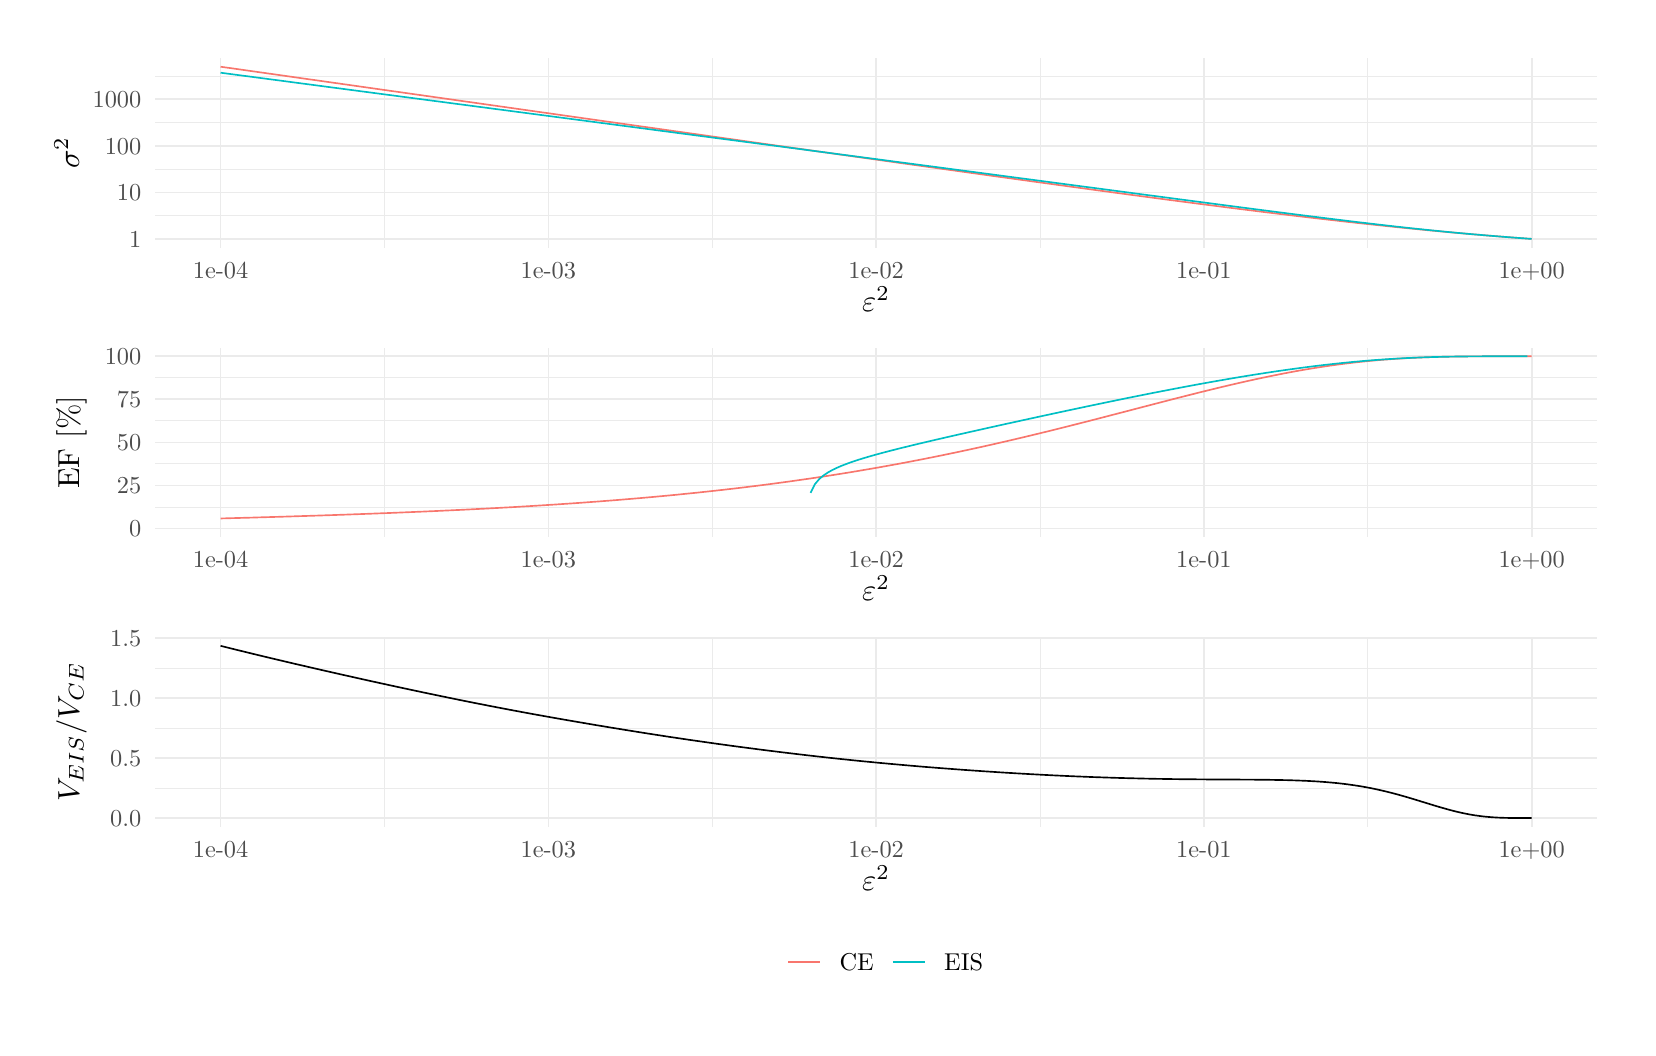
\begin{tikzpicture}[x=1pt,y=1pt]
\definecolor{fillColor}{RGB}{255,255,255}
\path[use as bounding box,fill=fillColor,fill opacity=0.00] (0,0) rectangle (578.16,361.35);
\begin{scope}
\path[clip] ( 46.01,281.90) rectangle (567.16,350.35);
\definecolor{drawColor}{gray}{0.92}

\path[draw=drawColor,line width= 0.3pt,line join=round] ( 46.01,293.43) --
	(567.16,293.43);

\path[draw=drawColor,line width= 0.3pt,line join=round] ( 46.01,310.25) --
	(567.16,310.25);

\path[draw=drawColor,line width= 0.3pt,line join=round] ( 46.01,327.07) --
	(567.16,327.07);

\path[draw=drawColor,line width= 0.3pt,line join=round] ( 46.01,343.89) --
	(567.16,343.89);

\path[draw=drawColor,line width= 0.3pt,line join=round] (128.92,281.90) --
	(128.92,350.35);

\path[draw=drawColor,line width= 0.3pt,line join=round] (247.36,281.90) --
	(247.36,350.35);

\path[draw=drawColor,line width= 0.3pt,line join=round] (365.81,281.90) --
	(365.81,350.35);

\path[draw=drawColor,line width= 0.3pt,line join=round] (484.25,281.90) --
	(484.25,350.35);

\path[draw=drawColor,line width= 0.6pt,line join=round] ( 46.01,285.02) --
	(567.16,285.02);

\path[draw=drawColor,line width= 0.6pt,line join=round] ( 46.01,301.84) --
	(567.16,301.84);

\path[draw=drawColor,line width= 0.6pt,line join=round] ( 46.01,318.66) --
	(567.16,318.66);

\path[draw=drawColor,line width= 0.6pt,line join=round] ( 46.01,335.48) --
	(567.16,335.48);

\path[draw=drawColor,line width= 0.6pt,line join=round] ( 69.70,281.90) --
	( 69.70,350.35);

\path[draw=drawColor,line width= 0.6pt,line join=round] (188.14,281.90) --
	(188.14,350.35);

\path[draw=drawColor,line width= 0.6pt,line join=round] (306.59,281.90) --
	(306.59,350.35);

\path[draw=drawColor,line width= 0.6pt,line join=round] (425.03,281.90) --
	(425.03,350.35);

\path[draw=drawColor,line width= 0.6pt,line join=round] (543.47,281.90) --
	(543.47,350.35);
\definecolor{drawColor}{RGB}{248,118,109}

\path[draw=drawColor,line width= 0.6pt,line join=round] ( 69.70,347.24) --
	( 71.28,347.01) --
	( 72.86,346.79) --
	( 74.44,346.57) --
	( 76.02,346.34) --
	( 77.59,346.12) --
	( 79.17,345.89) --
	( 80.75,345.67) --
	( 82.33,345.45) --
	( 83.91,345.22) --
	( 85.49,345.00) --
	( 87.07,344.77) --
	( 88.65,344.55) --
	( 90.23,344.32) --
	( 91.81,344.10) --
	( 93.39,343.88) --
	( 94.97,343.65) --
	( 96.55,343.43) --
	( 98.13,343.20) --
	( 99.70,342.98) --
	(101.28,342.75) --
	(102.86,342.53) --
	(104.44,342.31) --
	(106.02,342.08) --
	(107.60,341.86) --
	(109.18,341.63) --
	(110.76,341.41) --
	(112.34,341.19) --
	(113.92,340.96) --
	(115.50,340.74) --
	(117.08,340.51) --
	(118.66,340.29) --
	(120.23,340.06) --
	(121.81,339.84) --
	(123.39,339.62) --
	(124.97,339.39) --
	(126.55,339.17) --
	(128.13,338.94) --
	(129.71,338.72) --
	(131.29,338.49) --
	(132.87,338.27) --
	(134.45,338.05) --
	(136.03,337.82) --
	(137.61,337.60) --
	(139.19,337.37) --
	(140.76,337.15) --
	(142.34,336.93) --
	(143.92,336.70) --
	(145.50,336.48) --
	(147.08,336.25) --
	(148.66,336.03) --
	(150.24,335.80) --
	(151.82,335.58) --
	(153.40,335.36) --
	(154.98,335.13) --
	(156.56,334.91) --
	(158.14,334.68) --
	(159.72,334.46) --
	(161.29,334.24) --
	(162.87,334.01) --
	(164.45,333.79) --
	(166.03,333.56) --
	(167.61,333.34) --
	(169.19,333.12) --
	(170.77,332.89) --
	(172.35,332.67) --
	(173.93,332.44) --
	(175.51,332.22) --
	(177.09,331.99) --
	(178.67,331.77) --
	(180.25,331.55) --
	(181.82,331.32) --
	(183.40,331.10) --
	(184.98,330.87) --
	(186.56,330.65) --
	(188.14,330.43) --
	(189.72,330.20) --
	(191.30,329.98) --
	(192.88,329.75) --
	(194.46,329.53) --
	(196.04,329.31) --
	(197.62,329.08) --
	(199.20,328.86) --
	(200.78,328.63) --
	(202.36,328.41) --
	(203.93,328.19) --
	(205.51,327.96) --
	(207.09,327.74) --
	(208.67,327.51) --
	(210.25,327.29) --
	(211.83,327.07) --
	(213.41,326.84) --
	(214.99,326.62) --
	(216.57,326.40) --
	(218.15,326.17) --
	(219.73,325.95) --
	(221.31,325.72) --
	(222.89,325.50) --
	(224.46,325.28) --
	(226.04,325.05) --
	(227.62,324.83) --
	(229.20,324.60) --
	(230.78,324.38) --
	(232.36,324.16) --
	(233.94,323.93) --
	(235.52,323.71) --
	(237.10,323.49) --
	(238.68,323.26) --
	(240.26,323.04) --
	(241.84,322.82) --
	(243.42,322.59) --
	(244.99,322.37) --
	(246.57,322.14) --
	(248.15,321.92) --
	(249.73,321.70) --
	(251.31,321.47) --
	(252.89,321.25) --
	(254.47,321.03) --
	(256.05,320.80) --
	(257.63,320.58) --
	(259.21,320.36) --
	(260.79,320.13) --
	(262.37,319.91) --
	(263.95,319.69) --
	(265.52,319.46) --
	(267.10,319.24) --
	(268.68,319.02) --
	(270.26,318.79) --
	(271.84,318.57) --
	(273.42,318.35) --
	(275.00,318.12) --
	(276.58,317.90) --
	(278.16,317.68) --
	(279.74,317.46) --
	(281.32,317.23) --
	(282.90,317.01) --
	(284.48,316.79) --
	(286.05,316.56) --
	(287.63,316.34) --
	(289.21,316.12) --
	(290.79,315.90) --
	(292.37,315.67) --
	(293.95,315.45) --
	(295.53,315.23) --
	(297.11,315.01) --
	(298.69,314.78) --
	(300.27,314.56) --
	(301.85,314.34) --
	(303.43,314.12) --
	(305.01,313.90) --
	(306.59,313.67) --
	(308.16,313.45) --
	(309.74,313.23) --
	(311.32,313.01) --
	(312.90,312.79) --
	(314.48,312.56) --
	(316.06,312.34) --
	(317.64,312.12) --
	(319.22,311.90) --
	(320.80,311.68) --
	(322.38,311.46) --
	(323.96,311.24) --
	(325.54,311.01) --
	(327.12,310.79) --
	(328.69,310.57) --
	(330.27,310.35) --
	(331.85,310.13) --
	(333.43,309.91) --
	(335.01,309.69) --
	(336.59,309.47) --
	(338.17,309.25) --
	(339.75,309.03) --
	(341.33,308.81) --
	(342.91,308.59) --
	(344.49,308.37) --
	(346.07,308.15) --
	(347.65,307.93) --
	(349.22,307.71) --
	(350.80,307.49) --
	(352.38,307.27) --
	(353.96,307.05) --
	(355.54,306.84) --
	(357.12,306.62) --
	(358.70,306.40) --
	(360.28,306.18) --
	(361.86,305.96) --
	(363.44,305.74) --
	(365.02,305.53) --
	(366.60,305.31) --
	(368.18,305.09) --
	(369.75,304.88) --
	(371.33,304.66) --
	(372.91,304.44) --
	(374.49,304.23) --
	(376.07,304.01) --
	(377.65,303.79) --
	(379.23,303.58) --
	(380.81,303.36) --
	(382.39,303.15) --
	(383.97,302.93) --
	(385.55,302.72) --
	(387.13,302.50) --
	(388.71,302.29) --
	(390.28,302.08) --
	(391.86,301.86) --
	(393.44,301.65) --
	(395.02,301.44) --
	(396.60,301.23) --
	(398.18,301.01) --
	(399.76,300.80) --
	(401.34,300.59) --
	(402.92,300.38) --
	(404.50,300.17) --
	(406.08,299.96) --
	(407.66,299.75) --
	(409.24,299.54) --
	(410.82,299.33) --
	(412.39,299.12) --
	(413.97,298.92) --
	(415.55,298.71) --
	(417.13,298.50) --
	(418.71,298.30) --
	(420.29,298.09) --
	(421.87,297.88) --
	(423.45,297.68) --
	(425.03,297.48) --
	(426.61,297.27) --
	(428.19,297.07) --
	(429.77,296.87) --
	(431.35,296.67) --
	(432.92,296.46) --
	(434.50,296.26) --
	(436.08,296.06) --
	(437.66,295.86) --
	(439.24,295.67) --
	(440.82,295.47) --
	(442.40,295.27) --
	(443.98,295.07) --
	(445.56,294.88) --
	(447.14,294.68) --
	(448.72,294.49) --
	(450.30,294.30) --
	(451.88,294.10) --
	(453.45,293.91) --
	(455.03,293.72) --
	(456.61,293.53) --
	(458.19,293.34) --
	(459.77,293.16) --
	(461.35,292.97) --
	(462.93,292.78) --
	(464.51,292.60) --
	(466.09,292.41) --
	(467.67,292.23) --
	(469.25,292.05) --
	(470.83,291.87) --
	(472.41,291.69) --
	(473.98,291.51) --
	(475.56,291.33) --
	(477.14,291.15) --
	(478.72,290.98) --
	(480.30,290.80) --
	(481.88,290.63) --
	(483.46,290.46) --
	(485.04,290.29) --
	(486.62,290.12) --
	(488.20,289.95) --
	(489.78,289.79) --
	(491.36,289.62) --
	(492.94,289.46) --
	(494.51,289.29) --
	(496.09,289.13) --
	(497.67,288.97) --
	(499.25,288.81) --
	(500.83,288.66) --
	(502.41,288.50) --
	(503.99,288.35) --
	(505.57,288.19) --
	(507.15,288.04) --
	(508.73,287.89) --
	(510.31,287.75) --
	(511.89,287.60) --
	(513.47,287.45) --
	(515.05,287.31) --
	(516.62,287.17) --
	(518.20,287.03) --
	(519.78,286.89) --
	(521.36,286.75) --
	(522.94,286.62) --
	(524.52,286.49) --
	(526.10,286.35) --
	(527.68,286.22) --
	(529.26,286.10) --
	(530.84,285.97) --
	(532.42,285.84) --
	(534.00,285.72) --
	(535.58,285.60) --
	(537.15,285.48) --
	(538.73,285.36) --
	(540.31,285.24) --
	(541.89,285.13) --
	(543.47,285.02);
\definecolor{drawColor}{RGB}{0,191,196}

\path[draw=drawColor,line width= 0.6pt,line join=round] ( 69.70,345.07) --
	( 71.28,344.86) --
	( 72.86,344.65) --
	( 74.44,344.44) --
	( 76.02,344.23) --
	( 77.59,344.02) --
	( 79.17,343.82) --
	( 80.75,343.61) --
	( 82.33,343.40) --
	( 83.91,343.19) --
	( 85.49,342.98) --
	( 87.07,342.77) --
	( 88.65,342.56) --
	( 90.23,342.36) --
	( 91.81,342.15) --
	( 93.39,341.94) --
	( 94.97,341.73) --
	( 96.55,341.52) --
	( 98.13,341.31) --
	( 99.70,341.10) --
	(101.28,340.90) --
	(102.86,340.69) --
	(104.44,340.48) --
	(106.02,340.27) --
	(107.60,340.06) --
	(109.18,339.85) --
	(110.76,339.64) --
	(112.34,339.44) --
	(113.92,339.23) --
	(115.50,339.02) --
	(117.08,338.81) --
	(118.66,338.60) --
	(120.23,338.39) --
	(121.81,338.19) --
	(123.39,337.98) --
	(124.97,337.77) --
	(126.55,337.56) --
	(128.13,337.35) --
	(129.71,337.14) --
	(131.29,336.94) --
	(132.87,336.73) --
	(134.45,336.52) --
	(136.03,336.31) --
	(137.61,336.10) --
	(139.19,335.90) --
	(140.76,335.69) --
	(142.34,335.48) --
	(143.92,335.27) --
	(145.50,335.06) --
	(147.08,334.85) --
	(148.66,334.65) --
	(150.24,334.44) --
	(151.82,334.23) --
	(153.40,334.02) --
	(154.98,333.81) --
	(156.56,333.61) --
	(158.14,333.40) --
	(159.72,333.19) --
	(161.29,332.98) --
	(162.87,332.77) --
	(164.45,332.57) --
	(166.03,332.36) --
	(167.61,332.15) --
	(169.19,331.94) --
	(170.77,331.73) --
	(172.35,331.53) --
	(173.93,331.32) --
	(175.51,331.11) --
	(177.09,330.90) --
	(178.67,330.70) --
	(180.25,330.49) --
	(181.82,330.28) --
	(183.40,330.07) --
	(184.98,329.86) --
	(186.56,329.66) --
	(188.14,329.45) --
	(189.72,329.24) --
	(191.30,329.03) --
	(192.88,328.82) --
	(194.46,328.62) --
	(196.04,328.41) --
	(197.62,328.20) --
	(199.20,327.99) --
	(200.78,327.79) --
	(202.36,327.58) --
	(203.93,327.37) --
	(205.51,327.16) --
	(207.09,326.95) --
	(208.67,326.75) --
	(210.25,326.54) --
	(211.83,326.33) --
	(213.41,326.12) --
	(214.99,325.91) --
	(216.57,325.71) --
	(218.15,325.50) --
	(219.73,325.29) --
	(221.31,325.08) --
	(222.89,324.88) --
	(224.46,324.67) --
	(226.04,324.46) --
	(227.62,324.25) --
	(229.20,324.04) --
	(230.78,323.84) --
	(232.36,323.63) --
	(233.94,323.42) --
	(235.52,323.21) --
	(237.10,323.00) --
	(238.68,322.80) --
	(240.26,322.59) --
	(241.84,322.38) --
	(243.42,322.17) --
	(244.99,321.97) --
	(246.57,321.76) --
	(248.15,321.55) --
	(249.73,321.34) --
	(251.31,321.13) --
	(252.89,320.93) --
	(254.47,320.72) --
	(256.05,320.51) --
	(257.63,320.30) --
	(259.21,320.09) --
	(260.79,319.89) --
	(262.37,319.68) --
	(263.95,319.47) --
	(265.52,319.26) --
	(267.10,319.05) --
	(268.68,318.85) --
	(270.26,318.64) --
	(271.84,318.43) --
	(273.42,318.22) --
	(275.00,318.01) --
	(276.58,317.81) --
	(278.16,317.60) --
	(279.74,317.39) --
	(281.32,317.18) --
	(282.90,316.97) --
	(284.48,316.76) --
	(286.05,316.56) --
	(287.63,316.35) --
	(289.21,316.14) --
	(290.79,315.93) --
	(292.37,315.72) --
	(293.95,315.51) --
	(295.53,315.31) --
	(297.11,315.10) --
	(298.69,314.89) --
	(300.27,314.68) --
	(301.85,314.47) --
	(303.43,314.26) --
	(305.01,314.06) --
	(306.59,313.85) --
	(308.16,313.64) --
	(309.74,313.43) --
	(311.32,313.22) --
	(312.90,313.01) --
	(314.48,312.80) --
	(316.06,312.60) --
	(317.64,312.39) --
	(319.22,312.18) --
	(320.80,311.97) --
	(322.38,311.76) --
	(323.96,311.55) --
	(325.54,311.34) --
	(327.12,311.14) --
	(328.69,310.93) --
	(330.27,310.72) --
	(331.85,310.51) --
	(333.43,310.30) --
	(335.01,310.09) --
	(336.59,309.88) --
	(338.17,309.67) --
	(339.75,309.46) --
	(341.33,309.26) --
	(342.91,309.05) --
	(344.49,308.84) --
	(346.07,308.63) --
	(347.65,308.42) --
	(349.22,308.21) --
	(350.80,308.00) --
	(352.38,307.79) --
	(353.96,307.58) --
	(355.54,307.37) --
	(357.12,307.16) --
	(358.70,306.95) --
	(360.28,306.75) --
	(361.86,306.54) --
	(363.44,306.33) --
	(365.02,306.12) --
	(366.60,305.91) --
	(368.18,305.70) --
	(369.75,305.49) --
	(371.33,305.28) --
	(372.91,305.07) --
	(374.49,304.86) --
	(376.07,304.65) --
	(377.65,304.44) --
	(379.23,304.23) --
	(380.81,304.02) --
	(382.39,303.81) --
	(383.97,303.61) --
	(385.55,303.40) --
	(387.13,303.19) --
	(388.71,302.98) --
	(390.28,302.77) --
	(391.86,302.56) --
	(393.44,302.35) --
	(395.02,302.14) --
	(396.60,301.93) --
	(398.18,301.72) --
	(399.76,301.51) --
	(401.34,301.30) --
	(402.92,301.09) --
	(404.50,300.88) --
	(406.08,300.68) --
	(407.66,300.47) --
	(409.24,300.26) --
	(410.82,300.05) --
	(412.39,299.84) --
	(413.97,299.63) --
	(415.55,299.42) --
	(417.13,299.21) --
	(418.71,299.01) --
	(420.29,298.80) --
	(421.87,298.59) --
	(423.45,298.38) --
	(425.03,298.17) --
	(426.61,297.97) --
	(428.19,297.76) --
	(429.77,297.55) --
	(431.35,297.34) --
	(432.92,297.14) --
	(434.50,296.93) --
	(436.08,296.72) --
	(437.66,296.52) --
	(439.24,296.31) --
	(440.82,296.11) --
	(442.40,295.90) --
	(443.98,295.69) --
	(445.56,295.49) --
	(447.14,295.28) --
	(448.72,295.08) --
	(450.30,294.88) --
	(451.88,294.67) --
	(453.45,294.47) --
	(455.03,294.27) --
	(456.61,294.07) --
	(458.19,293.87) --
	(459.77,293.66) --
	(461.35,293.46) --
	(462.93,293.26) --
	(464.51,293.07) --
	(466.09,292.87) --
	(467.67,292.67) --
	(469.25,292.47) --
	(470.83,292.28) --
	(472.41,292.08) --
	(473.98,291.89) --
	(475.56,291.70) --
	(477.14,291.50) --
	(478.72,291.31) --
	(480.30,291.12) --
	(481.88,290.93) --
	(483.46,290.75) --
	(485.04,290.56) --
	(486.62,290.38) --
	(488.20,290.19) --
	(489.78,290.01) --
	(491.36,289.83) --
	(492.94,289.65) --
	(494.51,289.47) --
	(496.09,289.30) --
	(497.67,289.12) --
	(499.25,288.95) --
	(500.83,288.78) --
	(502.41,288.62) --
	(503.99,288.45) --
	(505.57,288.29) --
	(507.15,288.12) --
	(508.73,287.97) --
	(510.31,287.81) --
	(511.89,287.65) --
	(513.47,287.50) --
	(515.05,287.35) --
	(516.62,287.20) --
	(518.20,287.06) --
	(519.78,286.91) --
	(521.36,286.77) --
	(522.94,286.63) --
	(524.52,286.50) --
	(526.10,286.36) --
	(527.68,286.23) --
	(529.26,286.10) --
	(530.84,285.97) --
	(532.42,285.85) --
	(534.00,285.72) --
	(535.58,285.60) --
	(537.15,285.48) --
	(538.73,285.36) --
	(540.31,285.25) --
	(541.89,285.13) --
	(543.47,285.02);
\end{scope}
\begin{scope}
\path[clip] (  0.00,  0.00) rectangle (578.16,361.35);
\definecolor{drawColor}{gray}{0.30}

\node[text=drawColor,anchor=base east,inner sep=0pt, outer sep=0pt, scale=  0.88] at ( 41.06,281.99) {1};

\node[text=drawColor,anchor=base east,inner sep=0pt, outer sep=0pt, scale=  0.88] at ( 41.06,298.81) {10};

\node[text=drawColor,anchor=base east,inner sep=0pt, outer sep=0pt, scale=  0.88] at ( 41.06,315.63) {100};

\node[text=drawColor,anchor=base east,inner sep=0pt, outer sep=0pt, scale=  0.88] at ( 41.06,332.45) {1000};
\end{scope}
\begin{scope}
\path[clip] (  0.00,  0.00) rectangle (578.16,361.35);
\definecolor{drawColor}{gray}{0.30}

\node[text=drawColor,anchor=base,inner sep=0pt, outer sep=0pt, scale=  0.88] at ( 69.70,270.89) {1e-04};

\node[text=drawColor,anchor=base,inner sep=0pt, outer sep=0pt, scale=  0.88] at (188.14,270.89) {1e-03};

\node[text=drawColor,anchor=base,inner sep=0pt, outer sep=0pt, scale=  0.88] at (306.59,270.89) {1e-02};

\node[text=drawColor,anchor=base,inner sep=0pt, outer sep=0pt, scale=  0.88] at (425.03,270.89) {1e-01};

\node[text=drawColor,anchor=base,inner sep=0pt, outer sep=0pt, scale=  0.88] at (543.47,270.89) {1e+00};
\end{scope}
\begin{scope}
\path[clip] (  0.00,  0.00) rectangle (578.16,361.35);
\definecolor{drawColor}{RGB}{0,0,0}

\node[text=drawColor,anchor=base,inner sep=0pt, outer sep=0pt, scale=  1.10] at (306.59,258.86) {$\varepsilon^2$};
\end{scope}
\begin{scope}
\path[clip] (  0.00,  0.00) rectangle (578.16,361.35);
\definecolor{drawColor}{RGB}{0,0,0}

\node[text=drawColor,rotate= 90.00,anchor=base,inner sep=0pt, outer sep=0pt, scale=  1.10] at ( 18.58,316.13) {$\sigma^2$};
\end{scope}
\begin{scope}
\path[clip] ( 46.01,177.27) rectangle (567.16,245.72);
\definecolor{drawColor}{gray}{0.92}

\path[draw=drawColor,line width= 0.3pt,line join=round] ( 46.01,188.16) --
	(567.16,188.16);

\path[draw=drawColor,line width= 0.3pt,line join=round] ( 46.01,203.72) --
	(567.16,203.72);

\path[draw=drawColor,line width= 0.3pt,line join=round] ( 46.01,219.27) --
	(567.16,219.27);

\path[draw=drawColor,line width= 0.3pt,line join=round] ( 46.01,234.83) --
	(567.16,234.83);

\path[draw=drawColor,line width= 0.3pt,line join=round] (128.92,177.27) --
	(128.92,245.72);

\path[draw=drawColor,line width= 0.3pt,line join=round] (247.36,177.27) --
	(247.36,245.72);

\path[draw=drawColor,line width= 0.3pt,line join=round] (365.81,177.27) --
	(365.81,245.72);

\path[draw=drawColor,line width= 0.3pt,line join=round] (484.25,177.27) --
	(484.25,245.72);

\path[draw=drawColor,line width= 0.6pt,line join=round] ( 46.01,180.38) --
	(567.16,180.38);

\path[draw=drawColor,line width= 0.6pt,line join=round] ( 46.01,195.94) --
	(567.16,195.94);

\path[draw=drawColor,line width= 0.6pt,line join=round] ( 46.01,211.49) --
	(567.16,211.49);

\path[draw=drawColor,line width= 0.6pt,line join=round] ( 46.01,227.05) --
	(567.16,227.05);

\path[draw=drawColor,line width= 0.6pt,line join=round] ( 46.01,242.61) --
	(567.16,242.61);

\path[draw=drawColor,line width= 0.6pt,line join=round] ( 69.70,177.27) --
	( 69.70,245.72);

\path[draw=drawColor,line width= 0.6pt,line join=round] (188.14,177.27) --
	(188.14,245.72);

\path[draw=drawColor,line width= 0.6pt,line join=round] (306.59,177.27) --
	(306.59,245.72);

\path[draw=drawColor,line width= 0.6pt,line join=round] (425.03,177.27) --
	(425.03,245.72);

\path[draw=drawColor,line width= 0.6pt,line join=round] (543.47,177.27) --
	(543.47,245.72);
\definecolor{drawColor}{RGB}{248,118,109}

\path[draw=drawColor,line width= 0.6pt,line join=round] ( 69.70,184.00) --
	( 71.28,184.04) --
	( 72.86,184.09) --
	( 74.44,184.13) --
	( 76.02,184.17) --
	( 77.59,184.22) --
	( 79.17,184.26) --
	( 80.75,184.30) --
	( 82.33,184.35) --
	( 83.91,184.40) --
	( 85.49,184.44) --
	( 87.07,184.49) --
	( 88.65,184.54) --
	( 90.23,184.58) --
	( 91.81,184.63) --
	( 93.39,184.68) --
	( 94.97,184.73) --
	( 96.55,184.78) --
	( 98.13,184.83) --
	( 99.70,184.88) --
	(101.28,184.93) --
	(102.86,184.98) --
	(104.44,185.03) --
	(106.02,185.08) --
	(107.60,185.14) --
	(109.18,185.19) --
	(110.76,185.24) --
	(112.34,185.30) --
	(113.92,185.35) --
	(115.50,185.41) --
	(117.08,185.47) --
	(118.66,185.52) --
	(120.23,185.58) --
	(121.81,185.64) --
	(123.39,185.70) --
	(124.97,185.76) --
	(126.55,185.82) --
	(128.13,185.88) --
	(129.71,185.94) --
	(131.29,186.00) --
	(132.87,186.07) --
	(134.45,186.13) --
	(136.03,186.20) --
	(137.61,186.26) --
	(139.19,186.33) --
	(140.76,186.40) --
	(142.34,186.46) --
	(143.92,186.53) --
	(145.50,186.60) --
	(147.08,186.67) --
	(148.66,186.74) --
	(150.24,186.82) --
	(151.82,186.89) --
	(153.40,186.96) --
	(154.98,187.04) --
	(156.56,187.11) --
	(158.14,187.19) --
	(159.72,187.27) --
	(161.29,187.35) --
	(162.87,187.43) --
	(164.45,187.51) --
	(166.03,187.59) --
	(167.61,187.68) --
	(169.19,187.76) --
	(170.77,187.85) --
	(172.35,187.94) --
	(173.93,188.02) --
	(175.51,188.11) --
	(177.09,188.20) --
	(178.67,188.30) --
	(180.25,188.39) --
	(181.82,188.49) --
	(183.40,188.58) --
	(184.98,188.68) --
	(186.56,188.78) --
	(188.14,188.88) --
	(189.72,188.98) --
	(191.30,189.08) --
	(192.88,189.19) --
	(194.46,189.30) --
	(196.04,189.40) --
	(197.62,189.51) --
	(199.20,189.62) --
	(200.78,189.74) --
	(202.36,189.85) --
	(203.93,189.97) --
	(205.51,190.08) --
	(207.09,190.20) --
	(208.67,190.33) --
	(210.25,190.45) --
	(211.83,190.57) --
	(213.41,190.70) --
	(214.99,190.83) --
	(216.57,190.96) --
	(218.15,191.09) --
	(219.73,191.23) --
	(221.31,191.36) --
	(222.89,191.50) --
	(224.46,191.64) --
	(226.04,191.78) --
	(227.62,191.93) --
	(229.20,192.07) --
	(230.78,192.22) --
	(232.36,192.37) --
	(233.94,192.52) --
	(235.52,192.68) --
	(237.10,192.84) --
	(238.68,193.00) --
	(240.26,193.16) --
	(241.84,193.32) --
	(243.42,193.49) --
	(244.99,193.66) --
	(246.57,193.83) --
	(248.15,194.00) --
	(249.73,194.18) --
	(251.31,194.35) --
	(252.89,194.54) --
	(254.47,194.72) --
	(256.05,194.90) --
	(257.63,195.09) --
	(259.21,195.28) --
	(260.79,195.48) --
	(262.37,195.67) --
	(263.95,195.87) --
	(265.52,196.07) --
	(267.10,196.27) --
	(268.68,196.48) --
	(270.26,196.69) --
	(271.84,196.90) --
	(273.42,197.12) --
	(275.00,197.33) --
	(276.58,197.55) --
	(278.16,197.78) --
	(279.74,198.00) --
	(281.32,198.23) --
	(282.90,198.46) --
	(284.48,198.70) --
	(286.05,198.93) --
	(287.63,199.17) --
	(289.21,199.42) --
	(290.79,199.66) --
	(292.37,199.91) --
	(293.95,200.16) --
	(295.53,200.42) --
	(297.11,200.67) --
	(298.69,200.94) --
	(300.27,201.20) --
	(301.85,201.47) --
	(303.43,201.74) --
	(305.01,202.01) --
	(306.59,202.28) --
	(308.16,202.56) --
	(309.74,202.85) --
	(311.32,203.13) --
	(312.90,203.42) --
	(314.48,203.71) --
	(316.06,204.00) --
	(317.64,204.30) --
	(319.22,204.60) --
	(320.80,204.91) --
	(322.38,205.21) --
	(323.96,205.52) --
	(325.54,205.84) --
	(327.12,206.15) --
	(328.69,206.47) --
	(330.27,206.79) --
	(331.85,207.12) --
	(333.43,207.45) --
	(335.01,207.78) --
	(336.59,208.11) --
	(338.17,208.45) --
	(339.75,208.79) --
	(341.33,209.13) --
	(342.91,209.48) --
	(344.49,209.82) --
	(346.07,210.18) --
	(347.65,210.53) --
	(349.22,210.89) --
	(350.80,211.25) --
	(352.38,211.61) --
	(353.96,211.97) --
	(355.54,212.34) --
	(357.12,212.71) --
	(358.70,213.09) --
	(360.28,213.46) --
	(361.86,213.84) --
	(363.44,214.22) --
	(365.02,214.60) --
	(366.60,214.99) --
	(368.18,215.37) --
	(369.75,215.76) --
	(371.33,216.15) --
	(372.91,216.55) --
	(374.49,216.94) --
	(376.07,217.34) --
	(377.65,217.74) --
	(379.23,218.14) --
	(380.81,218.54) --
	(382.39,218.94) --
	(383.97,219.35) --
	(385.55,219.75) --
	(387.13,220.16) --
	(388.71,220.57) --
	(390.28,220.98) --
	(391.86,221.39) --
	(393.44,221.80) --
	(395.02,222.21) --
	(396.60,222.62) --
	(398.18,223.03) --
	(399.76,223.45) --
	(401.34,223.86) --
	(402.92,224.27) --
	(404.50,224.68) --
	(406.08,225.09) --
	(407.66,225.50) --
	(409.24,225.91) --
	(410.82,226.32) --
	(412.39,226.73) --
	(413.97,227.14) --
	(415.55,227.54) --
	(417.13,227.94) --
	(418.71,228.35) --
	(420.29,228.74) --
	(421.87,229.14) --
	(423.45,229.54) --
	(425.03,229.93) --
	(426.61,230.32) --
	(428.19,230.70) --
	(429.77,231.09) --
	(431.35,231.47) --
	(432.92,231.84) --
	(434.50,232.22) --
	(436.08,232.58) --
	(437.66,232.95) --
	(439.24,233.31) --
	(440.82,233.66) --
	(442.40,234.01) --
	(443.98,234.36) --
	(445.56,234.70) --
	(447.14,235.03) --
	(448.72,235.36) --
	(450.30,235.68) --
	(451.88,236.00) --
	(453.45,236.31) --
	(455.03,236.61) --
	(456.61,236.91) --
	(458.19,237.20) --
	(459.77,237.48) --
	(461.35,237.76) --
	(462.93,238.02) --
	(464.51,238.28) --
	(466.09,238.54) --
	(467.67,238.78) --
	(469.25,239.02) --
	(470.83,239.25) --
	(472.41,239.47) --
	(473.98,239.68) --
	(475.56,239.89) --
	(477.14,240.08) --
	(478.72,240.27) --
	(480.30,240.45) --
	(481.88,240.62) --
	(483.46,240.78) --
	(485.04,240.94) --
	(486.62,241.08) --
	(488.20,241.22) --
	(489.78,241.35) --
	(491.36,241.47) --
	(492.94,241.59) --
	(494.51,241.70) --
	(496.09,241.79) --
	(497.67,241.89) --
	(499.25,241.97) --
	(500.83,242.05) --
	(502.41,242.12) --
	(503.99,242.19) --
	(505.57,242.24) --
	(507.15,242.30) --
	(508.73,242.34) --
	(510.31,242.39) --
	(511.89,242.42) --
	(513.47,242.46) --
	(515.05,242.48) --
	(516.62,242.51) --
	(518.20,242.53) --
	(519.78,242.55) --
	(521.36,242.56) --
	(522.94,242.57) --
	(524.52,242.58) --
	(526.10,242.59) --
	(527.68,242.59) --
	(529.26,242.60) --
	(530.84,242.60) --
	(532.42,242.60) --
	(534.00,242.61) --
	(535.58,242.61) --
	(537.15,242.61) --
	(538.73,242.61) --
	(540.31,242.61) --
	(541.89,242.61) --
	(543.47,242.61);
\definecolor{drawColor}{RGB}{0,191,196}

\path[draw=drawColor,line width= 0.6pt,line join=round] (282.90,193.24) --
	(284.48,196.41) --
	(286.05,198.26) --
	(287.63,199.59) --
	(289.21,200.64) --
	(290.79,201.52) --
	(292.37,202.28) --
	(293.95,202.97) --
	(295.53,203.59) --
	(297.11,204.17) --
	(298.69,204.72) --
	(300.27,205.23) --
	(301.85,205.72) --
	(303.43,206.19) --
	(305.01,206.65) --
	(306.59,207.09) --
	(308.16,207.52) --
	(309.74,207.94) --
	(311.32,208.36) --
	(312.90,208.76) --
	(314.48,209.16) --
	(316.06,209.56) --
	(317.64,209.94) --
	(319.22,210.33) --
	(320.80,210.71) --
	(322.38,211.09) --
	(323.96,211.46) --
	(325.54,211.83) --
	(327.12,212.20) --
	(328.69,212.57) --
	(330.27,212.93) --
	(331.85,213.30) --
	(333.43,213.66) --
	(335.01,214.02) --
	(336.59,214.38) --
	(338.17,214.73) --
	(339.75,215.09) --
	(341.33,215.45) --
	(342.91,215.80) --
	(344.49,216.15) --
	(346.07,216.51) --
	(347.65,216.86) --
	(349.22,217.21) --
	(350.80,217.56) --
	(352.38,217.91) --
	(353.96,218.26) --
	(355.54,218.60) --
	(357.12,218.95) --
	(358.70,219.30) --
	(360.28,219.64) --
	(361.86,219.99) --
	(363.44,220.33) --
	(365.02,220.68) --
	(366.60,221.02) --
	(368.18,221.36) --
	(369.75,221.70) --
	(371.33,222.04) --
	(372.91,222.38) --
	(374.49,222.72) --
	(376.07,223.06) --
	(377.65,223.39) --
	(379.23,223.73) --
	(380.81,224.06) --
	(382.39,224.40) --
	(383.97,224.73) --
	(385.55,225.06) --
	(387.13,225.39) --
	(388.71,225.72) --
	(390.28,226.05) --
	(391.86,226.37) --
	(393.44,226.70) --
	(395.02,227.02) --
	(396.60,227.35) --
	(398.18,227.67) --
	(399.76,227.99) --
	(401.34,228.30) --
	(402.92,228.62) --
	(404.50,228.93) --
	(406.08,229.25) --
	(407.66,229.56) --
	(409.24,229.87) --
	(410.82,230.17) --
	(412.39,230.48) --
	(413.97,230.78) --
	(415.55,231.08) --
	(417.13,231.38) --
	(418.71,231.68) --
	(420.29,231.97) --
	(421.87,232.27) --
	(423.45,232.56) --
	(425.03,232.84) --
	(426.61,233.13) --
	(428.19,233.41) --
	(429.77,233.69) --
	(431.35,233.96) --
	(432.92,234.24) --
	(434.50,234.51) --
	(436.08,234.78) --
	(437.66,235.04) --
	(439.24,235.30) --
	(440.82,235.56) --
	(442.40,235.82) --
	(443.98,236.07) --
	(445.56,236.31) --
	(447.14,236.56) --
	(448.72,236.80) --
	(450.30,237.04) --
	(451.88,237.27) --
	(453.45,237.50) --
	(455.03,237.72) --
	(456.61,237.94) --
	(458.19,238.16) --
	(459.77,238.37) --
	(461.35,238.58) --
	(462.93,238.78) --
	(464.51,238.98) --
	(466.09,239.18) --
	(467.67,239.37) --
	(469.25,239.55) --
	(470.83,239.73) --
	(472.41,239.90) --
	(473.98,240.07) --
	(475.56,240.24) --
	(477.14,240.39) --
	(478.72,240.55) --
	(480.30,240.69) --
	(481.88,240.83) --
	(483.46,240.97) --
	(485.04,241.10) --
	(486.62,241.22) --
	(488.20,241.34) --
	(489.78,241.45) --
	(491.36,241.56) --
	(492.94,241.66) --
	(494.51,241.76) --
	(496.09,241.84) --
	(497.67,241.93) --
	(499.25,242.00) --
	(500.83,242.07) --
	(502.41,242.14) --
	(503.99,242.20) --
	(505.57,242.26) --
	(507.15,242.31) --
	(508.73,242.35) --
	(510.31,242.39) --
	(511.89,242.43) --
	(513.47,242.46) --
	(515.05,242.49) --
	(516.62,242.51) --
	(518.20,242.53) --
	(519.78,242.55) --
	(521.36,242.56) --
	(522.94,242.57) --
	(524.52,242.58) --
	(526.10,242.59) --
	(527.68,242.59) --
	(529.26,242.60) --
	(530.84,242.60) --
	(532.42,242.60) --
	(534.00,242.61) --
	(535.58,242.61) --
	(537.15,242.61) --
	(538.73,242.61) --
	(540.31,242.61) --
	(541.89,242.61);
\end{scope}
\begin{scope}
\path[clip] (  0.00,  0.00) rectangle (578.16,361.35);
\definecolor{drawColor}{gray}{0.30}

\node[text=drawColor,anchor=base east,inner sep=0pt, outer sep=0pt, scale=  0.88] at ( 41.06,177.35) {0};

\node[text=drawColor,anchor=base east,inner sep=0pt, outer sep=0pt, scale=  0.88] at ( 41.06,192.91) {25};

\node[text=drawColor,anchor=base east,inner sep=0pt, outer sep=0pt, scale=  0.88] at ( 41.06,208.46) {50};

\node[text=drawColor,anchor=base east,inner sep=0pt, outer sep=0pt, scale=  0.88] at ( 41.06,224.02) {75};

\node[text=drawColor,anchor=base east,inner sep=0pt, outer sep=0pt, scale=  0.88] at ( 41.06,239.58) {100};
\end{scope}
\begin{scope}
\path[clip] (  0.00,  0.00) rectangle (578.16,361.35);
\definecolor{drawColor}{gray}{0.30}

\node[text=drawColor,anchor=base,inner sep=0pt, outer sep=0pt, scale=  0.88] at ( 69.70,166.26) {1e-04};

\node[text=drawColor,anchor=base,inner sep=0pt, outer sep=0pt, scale=  0.88] at (188.14,166.26) {1e-03};

\node[text=drawColor,anchor=base,inner sep=0pt, outer sep=0pt, scale=  0.88] at (306.59,166.26) {1e-02};

\node[text=drawColor,anchor=base,inner sep=0pt, outer sep=0pt, scale=  0.88] at (425.03,166.26) {1e-01};

\node[text=drawColor,anchor=base,inner sep=0pt, outer sep=0pt, scale=  0.88] at (543.47,166.26) {1e+00};
\end{scope}
\begin{scope}
\path[clip] (  0.00,  0.00) rectangle (578.16,361.35);
\definecolor{drawColor}{RGB}{0,0,0}

\node[text=drawColor,anchor=base,inner sep=0pt, outer sep=0pt, scale=  1.10] at (306.59,154.22) {$\varepsilon^2$};
\end{scope}
\begin{scope}
\path[clip] (  0.00,  0.00) rectangle (578.16,361.35);
\definecolor{drawColor}{RGB}{0,0,0}

\node[text=drawColor,rotate= 90.00,anchor=base,inner sep=0pt, outer sep=0pt, scale=  1.10] at ( 18.58,211.49) {EF [\%]};
\end{scope}
\begin{scope}
\path[clip] ( 46.01, 72.64) rectangle (567.16,141.09);
\definecolor{drawColor}{gray}{0.92}

\path[draw=drawColor,line width= 0.3pt,line join=round] ( 46.01, 86.59) --
	(567.16, 86.59);

\path[draw=drawColor,line width= 0.3pt,line join=round] ( 46.01,108.27) --
	(567.16,108.27);

\path[draw=drawColor,line width= 0.3pt,line join=round] ( 46.01,129.94) --
	(567.16,129.94);

\path[draw=drawColor,line width= 0.3pt,line join=round] (128.92, 72.64) --
	(128.92,141.09);

\path[draw=drawColor,line width= 0.3pt,line join=round] (247.36, 72.64) --
	(247.36,141.09);

\path[draw=drawColor,line width= 0.3pt,line join=round] (365.81, 72.64) --
	(365.81,141.09);

\path[draw=drawColor,line width= 0.3pt,line join=round] (484.25, 72.64) --
	(484.25,141.09);

\path[draw=drawColor,line width= 0.6pt,line join=round] ( 46.01, 75.75) --
	(567.16, 75.75);

\path[draw=drawColor,line width= 0.6pt,line join=round] ( 46.01, 97.43) --
	(567.16, 97.43);

\path[draw=drawColor,line width= 0.6pt,line join=round] ( 46.01,119.10) --
	(567.16,119.10);

\path[draw=drawColor,line width= 0.6pt,line join=round] ( 46.01,140.78) --
	(567.16,140.78);

\path[draw=drawColor,line width= 0.6pt,line join=round] ( 69.70, 72.64) --
	( 69.70,141.09);

\path[draw=drawColor,line width= 0.6pt,line join=round] (188.14, 72.64) --
	(188.14,141.09);

\path[draw=drawColor,line width= 0.6pt,line join=round] (306.59, 72.64) --
	(306.59,141.09);

\path[draw=drawColor,line width= 0.6pt,line join=round] (425.03, 72.64) --
	(425.03,141.09);

\path[draw=drawColor,line width= 0.6pt,line join=round] (543.47, 72.64) --
	(543.47,141.09);
\definecolor{drawColor}{RGB}{0,0,0}

\path[draw=drawColor,line width= 0.6pt,line join=round] ( 69.70,137.97) --
	( 71.28,137.58) --
	( 72.86,137.19) --
	( 74.44,136.80) --
	( 76.02,136.40) --
	( 77.59,136.02) --
	( 79.17,135.63) --
	( 80.75,135.25) --
	( 82.33,134.86) --
	( 83.91,134.48) --
	( 85.49,134.10) --
	( 87.07,133.72) --
	( 88.65,133.34) --
	( 90.23,132.97) --
	( 91.81,132.60) --
	( 93.39,132.22) --
	( 94.97,131.85) --
	( 96.55,131.48) --
	( 98.13,131.11) --
	( 99.70,130.75) --
	(101.28,130.38) --
	(102.86,130.02) --
	(104.44,129.65) --
	(106.02,129.29) --
	(107.60,128.93) --
	(109.18,128.57) --
	(110.76,128.21) --
	(112.34,127.85) --
	(113.92,127.49) --
	(115.50,127.14) --
	(117.08,126.79) --
	(118.66,126.43) --
	(120.23,126.08) --
	(121.81,125.73) --
	(123.39,125.37) --
	(124.97,125.03) --
	(126.55,124.68) --
	(128.13,124.33) --
	(129.71,123.99) --
	(131.29,123.64) --
	(132.87,123.30) --
	(134.45,122.96) --
	(136.03,122.62) --
	(137.61,122.28) --
	(139.19,121.94) --
	(140.76,121.61) --
	(142.34,121.27) --
	(143.92,120.94) --
	(145.50,120.61) --
	(147.08,120.28) --
	(148.66,119.95) --
	(150.24,119.62) --
	(151.82,119.30) --
	(153.40,118.97) --
	(154.98,118.65) --
	(156.56,118.33) --
	(158.14,118.01) --
	(159.72,117.70) --
	(161.29,117.38) --
	(162.87,117.07) --
	(164.45,116.76) --
	(166.03,116.45) --
	(167.61,116.14) --
	(169.19,115.84) --
	(170.77,115.53) --
	(172.35,115.23) --
	(173.93,114.93) --
	(175.51,114.63) --
	(177.09,114.34) --
	(178.67,114.04) --
	(180.25,113.75) --
	(181.82,113.46) --
	(183.40,113.17) --
	(184.98,112.89) --
	(186.56,112.60) --
	(188.14,112.32) --
	(189.72,112.04) --
	(191.30,111.76) --
	(192.88,111.48) --
	(194.46,111.21) --
	(196.04,110.93) --
	(197.62,110.66) --
	(199.20,110.39) --
	(200.78,110.12) --
	(202.36,109.85) --
	(203.93,109.58) --
	(205.51,109.31) --
	(207.09,109.05) --
	(208.67,108.79) --
	(210.25,108.52) --
	(211.83,108.26) --
	(213.41,108.01) --
	(214.99,107.75) --
	(216.57,107.49) --
	(218.15,107.24) --
	(219.73,106.98) --
	(221.31,106.73) --
	(222.89,106.48) --
	(224.46,106.23) --
	(226.04,105.99) --
	(227.62,105.74) --
	(229.20,105.50) --
	(230.78,105.25) --
	(232.36,105.01) --
	(233.94,104.78) --
	(235.52,104.54) --
	(237.10,104.31) --
	(238.68,104.07) --
	(240.26,103.84) --
	(241.84,103.61) --
	(243.42,103.39) --
	(244.99,103.16) --
	(246.57,102.94) --
	(248.15,102.71) --
	(249.73,102.49) --
	(251.31,102.28) --
	(252.89,102.06) --
	(254.47,101.84) --
	(256.05,101.63) --
	(257.63,101.42) --
	(259.21,101.21) --
	(260.79,101.00) --
	(262.37,100.80) --
	(263.95,100.59) --
	(265.52,100.39) --
	(267.10,100.19) --
	(268.68, 99.99) --
	(270.26, 99.80) --
	(271.84, 99.60) --
	(273.42, 99.41) --
	(275.00, 99.22) --
	(276.58, 99.03) --
	(278.16, 98.84) --
	(279.74, 98.66) --
	(281.32, 98.47) --
	(282.90, 98.29) --
	(284.48, 98.11) --
	(286.05, 97.93) --
	(287.63, 97.76) --
	(289.21, 97.58) --
	(290.79, 97.41) --
	(292.37, 97.24) --
	(293.95, 97.07) --
	(295.53, 96.91) --
	(297.11, 96.74) --
	(298.69, 96.58) --
	(300.27, 96.42) --
	(301.85, 96.26) --
	(303.43, 96.11) --
	(305.01, 95.96) --
	(306.59, 95.80) --
	(308.16, 95.65) --
	(309.74, 95.51) --
	(311.32, 95.36) --
	(312.90, 95.22) --
	(314.48, 95.08) --
	(316.06, 94.94) --
	(317.64, 94.80) --
	(319.22, 94.66) --
	(320.80, 94.53) --
	(322.38, 94.39) --
	(323.96, 94.26) --
	(325.54, 94.13) --
	(327.12, 94.01) --
	(328.69, 93.88) --
	(330.27, 93.76) --
	(331.85, 93.64) --
	(333.43, 93.52) --
	(335.01, 93.40) --
	(336.59, 93.28) --
	(338.17, 93.16) --
	(339.75, 93.05) --
	(341.33, 92.94) --
	(342.91, 92.83) --
	(344.49, 92.72) --
	(346.07, 92.61) --
	(347.65, 92.51) --
	(349.22, 92.41) --
	(350.80, 92.30) --
	(352.38, 92.20) --
	(353.96, 92.10) --
	(355.54, 92.01) --
	(357.12, 91.91) --
	(358.70, 91.82) --
	(360.28, 91.73) --
	(361.86, 91.64) --
	(363.44, 91.55) --
	(365.02, 91.47) --
	(366.60, 91.38) --
	(368.18, 91.30) --
	(369.75, 91.22) --
	(371.33, 91.14) --
	(372.91, 91.07) --
	(374.49, 90.99) --
	(376.07, 90.92) --
	(377.65, 90.85) --
	(379.23, 90.78) --
	(380.81, 90.72) --
	(382.39, 90.66) --
	(383.97, 90.59) --
	(385.55, 90.53) --
	(387.13, 90.48) --
	(388.71, 90.42) --
	(390.28, 90.37) --
	(391.86, 90.32) --
	(393.44, 90.27) --
	(395.02, 90.22) --
	(396.60, 90.18) --
	(398.18, 90.13) --
	(399.76, 90.10) --
	(401.34, 90.06) --
	(402.92, 90.02) --
	(404.50, 89.99) --
	(406.08, 89.95) --
	(407.66, 89.92) --
	(409.24, 89.90) --
	(410.82, 89.87) --
	(412.39, 89.85) --
	(413.97, 89.82) --
	(415.55, 89.80) --
	(417.13, 89.78) --
	(418.71, 89.77) --
	(420.29, 89.75) --
	(421.87, 89.74) --
	(423.45, 89.73) --
	(425.03, 89.71) --
	(426.61, 89.70) --
	(428.19, 89.69) --
	(429.77, 89.69) --
	(431.35, 89.68) --
	(432.92, 89.67) --
	(434.50, 89.66) --
	(436.08, 89.66) --
	(437.66, 89.65) --
	(439.24, 89.64) --
	(440.82, 89.63) --
	(442.40, 89.62) --
	(443.98, 89.61) --
	(445.56, 89.59) --
	(447.14, 89.58) --
	(448.72, 89.56) --
	(450.30, 89.53) --
	(451.88, 89.50) --
	(453.45, 89.47) --
	(455.03, 89.44) --
	(456.61, 89.39) --
	(458.19, 89.34) --
	(459.77, 89.28) --
	(461.35, 89.22) --
	(462.93, 89.14) --
	(464.51, 89.06) --
	(466.09, 88.96) --
	(467.67, 88.85) --
	(469.25, 88.73) --
	(470.83, 88.59) --
	(472.41, 88.45) --
	(473.98, 88.28) --
	(475.56, 88.10) --
	(477.14, 87.90) --
	(478.72, 87.68) --
	(480.30, 87.44) --
	(481.88, 87.19) --
	(483.46, 86.91) --
	(485.04, 86.61) --
	(486.62, 86.29) --
	(488.20, 85.95) --
	(489.78, 85.59) --
	(491.36, 85.21) --
	(492.94, 84.81) --
	(494.51, 84.40) --
	(496.09, 83.96) --
	(497.67, 83.51) --
	(499.25, 83.05) --
	(500.83, 82.57) --
	(502.41, 82.09) --
	(503.99, 81.60) --
	(505.57, 81.12) --
	(507.15, 80.63) --
	(508.73, 80.15) --
	(510.31, 79.68) --
	(511.89, 79.23) --
	(513.47, 78.79) --
	(515.05, 78.37) --
	(516.62, 77.98) --
	(518.20, 77.62) --
	(519.78, 77.29) --
	(521.36, 76.99) --
	(522.94, 76.73) --
	(524.52, 76.51) --
	(526.10, 76.31) --
	(527.68, 76.16) --
	(529.26, 76.03) --
	(530.84, 75.93) --
	(532.42, 75.86) --
	(534.00, 75.81) --
	(535.58, 75.78) --
	(537.15, 75.76) --
	(538.73, 75.76) --
	(540.31, 75.75) --
	(541.89, 75.75) --
	(543.47, 75.75);
\end{scope}
\begin{scope}
\path[clip] (  0.00,  0.00) rectangle (578.16,361.35);
\definecolor{drawColor}{gray}{0.30}

\node[text=drawColor,anchor=base east,inner sep=0pt, outer sep=0pt, scale=  0.88] at ( 41.06, 72.72) {0.0};

\node[text=drawColor,anchor=base east,inner sep=0pt, outer sep=0pt, scale=  0.88] at ( 41.06, 94.40) {0.5};

\node[text=drawColor,anchor=base east,inner sep=0pt, outer sep=0pt, scale=  0.88] at ( 41.06,116.07) {1.0};

\node[text=drawColor,anchor=base east,inner sep=0pt, outer sep=0pt, scale=  0.88] at ( 41.06,137.75) {1.5};
\end{scope}
\begin{scope}
\path[clip] (  0.00,  0.00) rectangle (578.16,361.35);
\definecolor{drawColor}{gray}{0.30}

\node[text=drawColor,anchor=base,inner sep=0pt, outer sep=0pt, scale=  0.88] at ( 69.70, 61.63) {1e-04};

\node[text=drawColor,anchor=base,inner sep=0pt, outer sep=0pt, scale=  0.88] at (188.14, 61.63) {1e-03};

\node[text=drawColor,anchor=base,inner sep=0pt, outer sep=0pt, scale=  0.88] at (306.59, 61.63) {1e-02};

\node[text=drawColor,anchor=base,inner sep=0pt, outer sep=0pt, scale=  0.88] at (425.03, 61.63) {1e-01};

\node[text=drawColor,anchor=base,inner sep=0pt, outer sep=0pt, scale=  0.88] at (543.47, 61.63) {1e+00};
\end{scope}
\begin{scope}
\path[clip] (  0.00,  0.00) rectangle (578.16,361.35);
\definecolor{drawColor}{RGB}{0,0,0}

\node[text=drawColor,anchor=base,inner sep=0pt, outer sep=0pt, scale=  1.10] at (306.59, 49.59) {$\varepsilon^2$};
\end{scope}
\begin{scope}
\path[clip] (  0.00,  0.00) rectangle (578.16,361.35);
\definecolor{drawColor}{RGB}{0,0,0}

\node[text=drawColor,rotate= 90.00,anchor=base,inner sep=0pt, outer sep=0pt, scale=  1.10] at ( 18.58,106.86) {$V_{EIS} / V_{CE}$};
\end{scope}
\begin{scope}
\path[clip] (  0.00,  0.00) rectangle (578.16,361.35);
\definecolor{drawColor}{RGB}{248,118,109}

\path[draw=drawColor,line width= 0.6pt,line join=round] (274.88, 23.73) -- (286.44, 23.73);
\end{scope}
\begin{scope}
\path[clip] (  0.00,  0.00) rectangle (578.16,361.35);
\definecolor{drawColor}{RGB}{0,191,196}

\path[draw=drawColor,line width= 0.6pt,line join=round] (312.68, 23.73) -- (324.24, 23.73);
\end{scope}
\begin{scope}
\path[clip] (  0.00,  0.00) rectangle (578.16,361.35);
\definecolor{drawColor}{RGB}{0,0,0}

\node[text=drawColor,anchor=base west,inner sep=0pt, outer sep=0pt, scale=  0.88] at (293.39, 20.70) {CE};
\end{scope}
\begin{scope}
\path[clip] (  0.00,  0.00) rectangle (578.16,361.35);
\definecolor{drawColor}{RGB}{0,0,0}

\node[text=drawColor,anchor=base west,inner sep=0pt, outer sep=0pt, scale=  0.88] at (331.18, 20.70) {EIS};
\end{scope}
\end{tikzpicture}
%
        }
        \caption{{\color{red} TODO}}
        \label{fig:gsmm_eps}
    \end{figure}

\end{example}

This is more of a technical counter-example, in practice the \gls{la} produces good importance sampling proposals, especially for \glspl{lcssm}. 

In the \gls{lcssm} setting \gls{eis} may produce invalid proposals, as estimates of the variance component in the weighted least squares regression are not guaranteed to be negative. Thus \gls{eis} may produce negative variances. To deal with this, the original \gls{eis} paper \cite[Section 3.2]{Richard2007Efficient} recommends either inflating the prior or setting the parameters in question to arbitrary fixed values. Alternatively using a more expensive constrained linear least squares solver, such as a conjugate-gradient method \cite{Branch1999Subspace} or the BVLS (bounded variable least squares) solver \cite{Stark1995Boundedvariable} may be appropriate, as is re-running the \gls{eis} procedure with a different random seed. Finally, in the \gls{lcssm} setting, we could also identify the corresponding observation as missing, similar to the argument presented in \Cref{subsec:glssm-approach} for the \gls{cem}. 

% CE failure?
The \gls{cem} presented in \Cref{subsec:markov-approach} (\Cref{alg:cem-markov-proposal-fast}) depends on the fact that the covariance matrix of the posterior $\cov \left( X | Y = y \right)$ is \gls{spd}, i.e. non-singular. This might be violated if, e.g., the model contains seasonal components whose associated innovations have variance $0$. In this case, the Cholesky roots involved will not be unique. Still \Cref{alg:cem-markov-proposal-fast} will, as $N\to\infty$ converge a globally optimal solution, though it may not be unique. 

\subsection{Computational complexity}
Throughout this section, we assume that the model in question is a \gls{lcssm} with linear signal (c.f. \Cref{def:lcssm}) to simplify the treatment. This benefits the \gls{la} and \gls{eis} approaches, as they may then be implemented in terms of the simulation and signal smoother. If the observation dimension $p$ is smaller than that of states $m$, this is more efficient and we'll assume this as well.
An overview of computational complexities is given in \Cref{tab:comparison-time-space-complexity}. Note that most operations can be parallelized in one way or the other, e.g. sampling from the proposals, and so the time-complexities are not necessarily indicative of real-world-performance. Still they provide theoretical insight into the performance of the three methods considered.

\begin{table}
    \centering
    \begin{tabular}{lccc}
        \toprule 
        method & single iteration (time) & single iteration (space) & simulation (time)\\
        \midrule
        \gls{la} & $\mathcal O (n \,p^{3})$ & $\mathcal O (np^{2})$ & $\mathcal O(n (p^{3} + m^{3} + N\,m^{2}))$ \\
        \gls{eis} & $\mathcal O (n(m^{2} + p^{3} + N\,p^{2}))$ & $\mathcal O (N\,p + n(p^{2} + m^{2}))$ & $\mathcal O(n (p^{3} + m^{3} + N\,m^{2}))$\\
        \gls{cem} & $\mathcal O (n (Nm^{2} + m^{4}))$& $\mathcal O (Nm + nm^{2})$ & $\mathcal O (N\,n\,m^{2})$\\
        \bottomrule
    \end{tabular}
    \caption{Computational complexities of importance sampling algorithms.}
    \label{tab:comparison-time-space-complexity}
\end{table}

% of fitting 
Let us begin with a discussion of the computational complexity involved in finding the optimal parameters, $\psi_{\la}, \hat\psi_{\eis}$ and $\hat\psi_{\ce}$. Here we focus on a single iteration and treat the number of iterations empirically in \Cref{subsec:numerical-convergence}.

As the \gls{la} is based on the Kalman-smoother, the time complexity of a single iteration is $\mathcal O(n(m^{2} + p^{3}))$. The \gls{cem} and \gls{eis} need to generate $N$ samples from the current proposal. For the \gls{cem} this amounts to $\mathcal O(N\,n\, m^{2})$ operations (see \Cref{subsec:markov-approach}). For \gls{eis}, using the simulation smoother \cite{Durbin2002Simple} requires $\mathcal O (n(m^{2} + p^{3} + N\,p^2))$ operations: we need to run the Kalman filter once, while preparing the matrices required for the simulation smoother. Then, provided Cholesky roots of the innovation covariance matrices $\Sigma_{t}$ are already available, only matrix-vector multiplications are necessary for the simulation smoother. Obtaining the \gls{eis} model parameters is efficient, requiring only $\mathcal O(n(N\,p^2 + p^{3}))$ operations for constructing the $n$ $p\times p$ design matrices and estimating the optimal parameters. 

% of simulation 
Another concern is the time required to generate $N$ samples from the fitted model. For both the \gls{la} and \gls{eis} this requires using either the simulation smoother or the FFBS algorithm. This necessitates inverting $p\times p$ matrices in the Kalman filter and $m \times m$ matrices when simulating the states. Fortunately, these steps can be performed offline, after which the simulation of a single sample requires only $\mathcal O(n)$ matrix-vector multiplications. The \gls{cem} simulation is based on applying \Cref{eq:markov-proposal}, which only requires $\mathcal O(n\,m^{2})$ time per sample. 

% of space
Concerning space complexity, the \gls{la} has to run the Kalman filter with $\mathcal O(n (p^{2} + m^{2}))$ space and store $\mathcal O(n p)$ parameters. 
\gls{eis} has the same space requirement, but needs additional $\mathcal O(Np)$ storage for the simulated signals. As the weights $w_{t}$ in \gls{eis} depend only on the current signals $S^{1}_{t}, \dots, S^{N}_{t}$, they may be discarded afterwards. See \Cref{subsec:markov-approach} for the derivation of the $\mathcal O(Nm + nm^{2})$ space requirement of the \gls{cem}.

% interpretation
The \gls{la} has the fastest and most space-efficient iteration of the three methods, because it does not require simulation of $N$ samples. This makes it an ideal candidate as an initial guess for the other two methods. 
% compare EIS vs. CEM
\todo{cem faster, only need $m^3$} For $p \ll m$, \gls{eis} is faster than \gls{cem} as it is based on the signals $S$ only, thus having access to the efficient simulation and signal smoother algorithms. The same is true for the space complexity. If, however, $p\approx m$, there is no linear signal or the observations are not conditionally independent given the states or signals, the speed of \gls{eis} and \gls{cem} should be comparable. 
% simulation
While theoretically, the \gls{cem} performs sampling faster than the other two methods, for large numbers of samples $N$ the difference is negligible because the additional computations only have to be performed once. 

\subsection{Asymptotic variance}
As we have seen in the previous section, the number of samples $N$ used to estimate $\pce$ and $\peis$ enter linearly into the computational complexities. Naturally, we want to know how big a sample size we should choose for our procedures and whether one of the two simulation-based procedures requires fewer samples than the other. To answer this question we turn to the two central limit theorems, \Cref{thm:ce-clt,thm:clt-eis}. If $N$ is large, the asymptotic variances (or rather: the asymptotic standard deviations) tell us how much stochastic variation we should expect around the optimal value, and can thus guide us in choosing $N$. 
We start with two examples in a univariate setting, where both the \gls{cem} and \gls{eis} use Gaussian proposals with either fixed variance (\Cref{ex:univ-gaussian-s2-fixed}) or mean (\Cref{ex:univ-gaussian-mu-fixed}).
This allows us to compare the methods for either the mean (variance) if the variance (mean) is fixed and potentially misspecified, i.e. not the global optimum. Additionally, the univariate setting allows us, in some cases, to derive analytical expressions of the efficiencies involved, allowing us to interpret them. \todo{rewrite this more clearly}

To compare both methods we will determine the asymptotic relative efficiencies, i.e. $ \frac{\var \left( \hpeis \right)}{\var \left( \hpce \right)}$, with values smaller than $1$ indicating that \gls{eis} requires (asymptotically) fewer samples for the same precision as the \gls{cem}.
Let us note that we are comparing the efficiencies of parameters $\psi$, not those of derived parameters such as the standard deviation or the \gls{ess}. However, should both methods have the same optimal value the relative efficiencies are the same for all parameters derived from $\psi$, by the delta method. By a continuity argument, the same is approximately true if the optimal values of the \gls{cem} and \gls{eis} are close.

\begin{example}[univariate Gaussian, $\sigma^{2}$ fixed]
    \label{ex:univ-gaussian-s2-fixed}
    Consider the probability space $ \left( \R, \mathcal B(\R), \P \right)$ where $\P = p\lambda$ for the Lebesgue measure $\lambda$ which is symmetric around $0$, i.e. $p(-x) = p(x)$ for $\lambda$-a.e. $x\in\R$ and possesses up to third order moments.
    Let $\G=\P$, so $W\equiv1$ and let $\G_{\psi} = \mathcal N \left( \sigma\psi, \sigma^{2} \right)$ be the single parameter natural exponential family of Gaussians with fixed variance $\sigma^{2} > 0$. Then 
    $$
    \log g_{\psi}(x) = \psi T(x) - \frac{\psi^{2}}{2} + \log h(x),
    $$
    where $T(x) = \frac{x}{\sigma}$ and $h(x)$ is the density of $\mathcal N(0, \sigma^{2})$ w.r.t. Lebesgue measure. 
    Note that $T$ is centered under $\P$. To compare the asymptotic behavior of the \gls{cem} and \gls{eis} we compute the asymptotic variances arising from their respective central limit theorems (\Cref{thm:ce-clt,thm:clt-eis}).

    By symmetry, both $\pce$ and $\peis$ are equal to $0$. 
    Then $I(\psi) = 1$ for all $\psi$, so 
    \begin{align}
    \label{eq:ce-gaussian-mean-var}
        V_{\ce} = \cov_{\P}(T) = \frac{\tau^{2}}{\sigma^{2}},
    \end{align}
    where $\tau^{2}=\P \operatorname{id}^{2}$ is the second moment of $\P$. 

    Additionally, $B_{\eis} = (\cov_{\P}(T))^{-1} = \frac{\sigma^{2}}{\tau^{2}}$ and
    \begin{align*}
    M_{\eis} &= \cov_{\P} \left( (\log \frac{p(x)}{h(x)} - \lambda_{\eis})T\right) \\
        &= \cov_{\P} \left(\left( \log p - \log h - \P (\log p - \log h) \right) T \right) \\
        &= \frac{1}{\sigma^{2}}\int p(x) x^{2}\left(\log p(x) + \frac{x^{2}}{2\sigma^{2}} - \P\left(\log p(x) + \frac{\tau^{2}}{2\sigma^{2}}\right)\right)^{2} \d x.
    \end{align*}
    Thus
    $$
    V_{\eis} = B_{\eis}M_{\eis}B_{\eis}= \sigma^{2}\frac{\gamma}{\tau^{4}},
    $$
    where $\gamma = \int p(x) x^{2}\left(\log p(x) + \frac{x^{2}}{2\sigma^{2}} - \P(\log p(x) + \frac{\tau^{2}}{2\sigma^{2}})\right)^{2} \d x.$
    
    Let us now consider three exemplary choices of $\P$ that illustrate a target that is sufficiently well-behaved (the standard normal), multimodal (a Gaussian location mixture) and has different behavior in the tails than indicated at the mode (a Gaussian scale mixture). 
    For each target, we vary $\sigma^{2}$ from $\frac{1}{2}$ to $3$ and obtain relative efficiencies of the \gls{cem} and \gls{eis} either analytically or by simulation, the results are shown in the left-hand side of \Cref{fig:are}.

    \begin{figure}
        \centering

        \resizebox{\textwidth}{!}{%
            % Created by tikzDevice version 0.12.6 on 2025-09-08 08:58:15
% !TEX encoding = UTF-8 Unicode
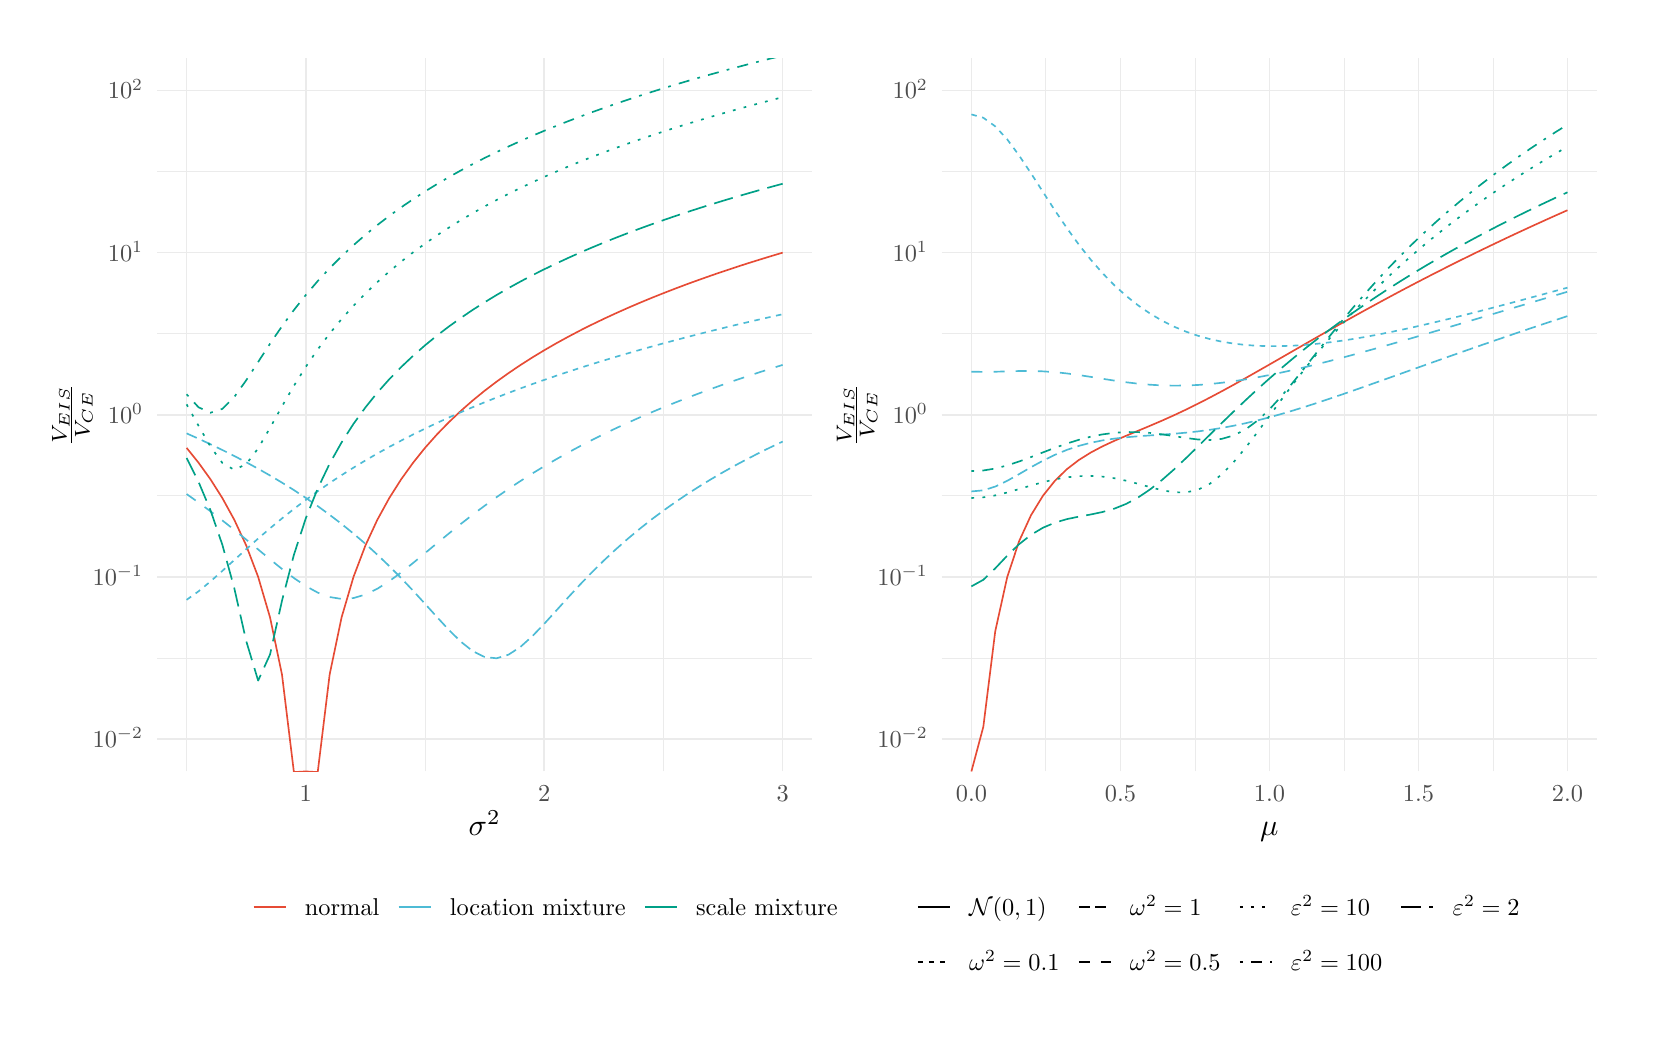
\begin{tikzpicture}[x=1pt,y=1pt]
\definecolor{fillColor}{RGB}{255,255,255}
\path[use as bounding box,fill=fillColor,fill opacity=0.00] (0,0) rectangle (578.16,361.35);
\begin{scope}
\path[clip] ( 46.66, 92.59) rectangle (283.58,350.35);
\definecolor{drawColor}{gray}{0.92}

\path[draw=drawColor,line width= 0.3pt,line join=round] ( 46.66,133.60) --
	(283.58,133.60);

\path[draw=drawColor,line width= 0.3pt,line join=round] ( 46.66,192.18) --
	(283.58,192.18);

\path[draw=drawColor,line width= 0.3pt,line join=round] ( 46.66,250.76) --
	(283.58,250.76);

\path[draw=drawColor,line width= 0.3pt,line join=round] ( 46.66,309.34) --
	(283.58,309.34);

\path[draw=drawColor,line width= 0.3pt,line join=round] ( 57.43, 92.59) --
	( 57.43,350.35);

\path[draw=drawColor,line width= 0.3pt,line join=round] (143.58, 92.59) --
	(143.58,350.35);

\path[draw=drawColor,line width= 0.3pt,line join=round] (229.74, 92.59) --
	(229.74,350.35);

\path[draw=drawColor,line width= 0.6pt,line join=round] ( 46.66,104.31) --
	(283.58,104.31);

\path[draw=drawColor,line width= 0.6pt,line join=round] ( 46.66,162.89) --
	(283.58,162.89);

\path[draw=drawColor,line width= 0.6pt,line join=round] ( 46.66,221.47) --
	(283.58,221.47);

\path[draw=drawColor,line width= 0.6pt,line join=round] ( 46.66,280.05) --
	(283.58,280.05);

\path[draw=drawColor,line width= 0.6pt,line join=round] ( 46.66,338.63) --
	(283.58,338.63);

\path[draw=drawColor,line width= 0.6pt,line join=round] (100.51, 92.59) --
	(100.51,350.35);

\path[draw=drawColor,line width= 0.6pt,line join=round] (186.66, 92.59) --
	(186.66,350.35);

\path[draw=drawColor,line width= 0.6pt,line join=round] (272.81, 92.59) --
	(272.81,350.35);
\definecolor{drawColor}{RGB}{230,75,53}

\path[draw=drawColor,line width= 0.6pt,line join=round] ( 57.43,209.51) --
	( 61.74,204.15) --
	( 66.05,198.16) --
	( 70.35,191.37) --
	( 74.66,183.52) --
	( 78.97,174.25) --
	( 83.28,162.89) --
	( 87.58,148.25) --
	( 91.89,127.62) --
	( 96.20, 92.35) --
	(100.51, 92.59) --
	(104.81, 92.35) --
	(109.12,127.62) --
	(113.43,148.25) --
	(117.74,162.89) --
	(122.05,174.25) --
	(126.35,183.52) --
	(130.66,191.37) --
	(134.97,198.16) --
	(139.28,204.15) --
	(143.58,209.51) --
	(147.89,214.36) --
	(152.20,218.79) --
	(156.51,222.86) --
	(160.81,226.63) --
	(165.12,230.15) --
	(169.43,233.43) --
	(173.74,236.51) --
	(178.04,239.42) --
	(182.35,242.17) --
	(186.66,244.78) --
	(190.97,247.27) --
	(195.27,249.63) --
	(199.58,251.90) --
	(203.89,254.06) --
	(208.20,256.14) --
	(212.50,258.13) --
	(216.81,260.05) --
	(221.12,261.90) --
	(225.43,263.69) --
	(229.74,265.41) --
	(234.04,267.08) --
	(238.35,268.70) --
	(242.66,270.26) --
	(246.97,271.78) --
	(251.27,273.26) --
	(255.58,274.69) --
	(259.89,276.09) --
	(264.20,277.44) --
	(268.50,278.76) --
	(272.81,280.05);
\definecolor{drawColor}{RGB}{77,187,213}

\path[draw=drawColor,line width= 0.6pt,dash pattern=on 2pt off 2pt ,line join=round] ( 57.43,154.60) --
	( 61.74,157.67) --
	( 66.05,161.24) --
	( 70.35,165.06) --
	( 74.66,168.99) --
	( 78.97,172.90) --
	( 83.28,176.74) --
	( 87.58,180.45) --
	( 91.89,184.02) --
	( 96.20,187.44) --
	(100.51,190.71) --
	(104.81,193.83) --
	(109.12,196.81) --
	(113.43,199.65) --
	(117.74,202.37) --
	(122.05,204.97) --
	(126.35,207.46) --
	(130.66,209.85) --
	(134.97,212.14) --
	(139.28,214.35) --
	(143.58,216.47) --
	(147.89,218.51) --
	(152.20,220.48) --
	(156.51,222.38) --
	(160.81,224.21) --
	(165.12,225.99) --
	(169.43,227.70) --
	(173.74,229.37) --
	(178.04,230.98) --
	(182.35,232.55) --
	(186.66,234.07) --
	(190.97,235.55) --
	(195.27,236.99) --
	(199.58,238.40) --
	(203.89,239.76) --
	(208.20,241.09) --
	(212.50,242.39) --
	(216.81,243.65) --
	(221.12,244.89) --
	(225.43,246.10) --
	(229.74,247.28) --
	(234.04,248.43) --
	(238.35,249.56) --
	(242.66,250.67) --
	(246.97,251.75) --
	(251.27,252.81) --
	(255.58,253.85) --
	(259.89,254.86) --
	(264.20,255.86) --
	(268.50,256.84) --
	(272.81,257.80);

\path[draw=drawColor,line width= 0.6pt,dash pattern=on 4pt off 2pt ,line join=round] ( 57.43,214.75) --
	( 61.74,212.82) --
	( 66.05,210.82) --
	( 70.35,208.74) --
	( 74.66,206.58) --
	( 78.97,204.32) --
	( 83.28,201.97) --
	( 87.58,199.52) --
	( 91.89,196.95) --
	( 96.20,194.26) --
	(100.51,191.43) --
	(104.81,188.46) --
	(109.12,185.32) --
	(113.43,182.02) --
	(117.74,178.52) --
	(122.05,174.83) --
	(126.35,170.92) --
	(130.66,166.79) --
	(134.97,162.44) --
	(139.28,157.88) --
	(143.58,153.16) --
	(147.89,148.39) --
	(152.20,143.73) --
	(156.51,139.49) --
	(160.81,136.06) --
	(165.12,133.94) --
	(169.43,133.47) --
	(173.74,134.77) --
	(178.04,137.57) --
	(182.35,141.45) --
	(186.66,145.93) --
	(190.97,150.67) --
	(195.27,155.44) --
	(199.58,160.09) --
	(203.89,164.55) --
	(208.20,168.80) --
	(212.50,172.82) --
	(216.81,176.63) --
	(221.12,180.22) --
	(225.43,183.63) --
	(229.74,186.85) --
	(234.04,189.90) --
	(238.35,192.80) --
	(242.66,195.56) --
	(246.97,198.20) --
	(251.27,200.71) --
	(255.58,203.11) --
	(259.89,205.42) --
	(264.20,207.62) --
	(268.50,209.75) --
	(272.81,211.79);

\path[draw=drawColor,line width= 0.6pt,dash pattern=on 4pt off 4pt ,line join=round] ( 57.43,192.82) --
	( 61.74,189.77) --
	( 66.05,186.59) --
	( 70.35,183.29) --
	( 74.66,179.88) --
	( 78.97,176.37) --
	( 83.28,172.81) --
	( 87.58,169.24) --
	( 91.89,165.76) --
	( 96.20,162.48) --
	(100.51,159.56) --
	(104.81,157.21) --
	(109.12,155.61) --
	(113.43,154.92) --
	(117.74,155.24) --
	(122.05,156.51) --
	(126.35,158.60) --
	(130.66,161.33) --
	(134.97,164.50) --
	(139.28,167.92) --
	(143.58,171.47) --
	(147.89,175.04) --
	(152.20,178.57) --
	(156.51,182.02) --
	(160.81,185.37) --
	(165.12,188.59) --
	(169.43,191.69) --
	(173.74,194.66) --
	(178.04,197.51) --
	(182.35,200.25) --
	(186.66,202.87) --
	(190.97,205.38) --
	(195.27,207.80) --
	(199.58,210.12) --
	(203.89,212.35) --
	(208.20,214.50) --
	(212.50,216.57) --
	(216.81,218.56) --
	(221.12,220.49) --
	(225.43,222.36) --
	(229.74,224.16) --
	(234.04,225.90) --
	(238.35,227.59) --
	(242.66,229.23) --
	(246.97,230.82) --
	(251.27,232.37) --
	(255.58,233.87) --
	(259.89,235.33) --
	(264.20,236.75) --
	(268.50,238.14) --
	(272.81,239.49);
\definecolor{drawColor}{RGB}{0,160,135}

\path[draw=drawColor,line width= 0.6pt,dash pattern=on 1pt off 3pt ,line join=round] ( 57.43,225.24) --
	( 61.74,217.50) --
	( 66.05,210.00) --
	( 70.35,204.05) --
	( 74.66,201.56) --
	( 78.97,203.63) --
	( 83.28,209.33) --
	( 87.58,216.75) --
	( 91.89,224.51) --
	( 96.20,231.93) --
	(100.51,238.80) --
	(104.81,245.08) --
	(109.12,250.81) --
	(113.43,256.05) --
	(117.74,260.86) --
	(122.05,265.30) --
	(126.35,269.41) --
	(130.66,273.23) --
	(134.97,276.81) --
	(139.28,280.16) --
	(143.58,283.31) --
	(147.89,286.29) --
	(152.20,289.10) --
	(156.51,291.78) --
	(160.81,294.32) --
	(165.12,296.75) --
	(169.43,299.07) --
	(173.74,301.29) --
	(178.04,303.42) --
	(182.35,305.46) --
	(186.66,307.43) --
	(190.97,309.32) --
	(195.27,311.15) --
	(199.58,312.91) --
	(203.89,314.62) --
	(208.20,316.27) --
	(212.50,317.87) --
	(216.81,319.43) --
	(221.12,320.93) --
	(225.43,322.40) --
	(229.74,323.82) --
	(234.04,325.21) --
	(238.35,326.55) --
	(242.66,327.87) --
	(246.97,329.15) --
	(251.27,330.40) --
	(255.58,331.62) --
	(259.89,332.81) --
	(264.20,333.97) --
	(268.50,335.11) --
	(272.81,336.23);

\path[draw=drawColor,line width= 0.6pt,dash pattern=on 1pt off 3pt on 4pt off 3pt ,line join=round] ( 57.43,228.88) --
	( 61.74,224.18) --
	( 66.05,222.19) --
	( 70.35,223.60) --
	( 74.66,227.92) --
	( 78.97,233.93) --
	( 83.28,240.55) --
	( 87.58,247.16) --
	( 91.89,253.45) --
	( 96.20,259.32) --
	(100.51,264.75) --
	(104.81,269.78) --
	(109.12,274.43) --
	(113.43,278.74) --
	(117.74,282.75) --
	(122.05,286.50) --
	(126.35,290.02) --
	(130.66,293.32) --
	(134.97,296.43) --
	(139.28,299.37) --
	(143.58,302.16) --
	(147.89,304.81) --
	(152.20,307.34) --
	(156.51,309.75) --
	(160.81,312.05) --
	(165.12,314.26) --
	(169.43,316.38) --
	(173.74,318.41) --
	(178.04,320.37) --
	(182.35,322.26) --
	(186.66,324.08) --
	(190.97,325.84) --
	(195.27,327.54) --
	(199.58,329.19) --
	(203.89,330.79) --
	(208.20,332.33) --
	(212.50,333.84) --
	(216.81,335.30) --
	(221.12,336.72) --
	(225.43,338.10) --
	(229.74,339.45) --
	(234.04,340.76) --
	(238.35,342.04) --
	(242.66,343.29) --
	(246.97,344.51) --
	(251.27,345.70) --
	(255.58,346.86) --
	(259.89,348.00) --
	(264.20,349.11) --
	(268.50,350.20) --
	(272.81,351.26);

\path[draw=drawColor,line width= 0.6pt,dash pattern=on 7pt off 3pt ,line join=round] ( 57.43,205.84) --
	( 61.74,197.23) --
	( 66.05,186.99) --
	( 70.35,174.47) --
	( 74.66,158.79) --
	( 78.97,139.71) --
	( 83.28,125.40) --
	( 87.58,134.87) --
	( 91.89,154.24) --
	( 96.20,170.86) --
	(100.51,184.08) --
	(104.81,194.82) --
	(109.12,203.80) --
	(113.43,211.48) --
	(117.74,218.19) --
	(122.05,224.13) --
	(126.35,229.47) --
	(130.66,234.30) --
	(134.97,238.72) --
	(139.28,242.79) --
	(143.58,246.56) --
	(147.89,250.08) --
	(152.20,253.36) --
	(156.51,256.45) --
	(160.81,259.37) --
	(165.12,262.12) --
	(169.43,264.74) --
	(173.74,267.23) --
	(178.04,269.60) --
	(182.35,271.87) --
	(186.66,274.04) --
	(190.97,276.12) --
	(195.27,278.12) --
	(199.58,280.05) --
	(203.89,281.90) --
	(208.20,283.69) --
	(212.50,285.42) --
	(216.81,287.09) --
	(221.12,288.71) --
	(225.43,290.28) --
	(229.74,291.80) --
	(234.04,293.28) --
	(238.35,294.72) --
	(242.66,296.12) --
	(246.97,297.48) --
	(251.27,298.80) --
	(255.58,300.09) --
	(259.89,301.35) --
	(264.20,302.58) --
	(268.50,303.78) --
	(272.81,304.95);
\end{scope}
\begin{scope}
\path[clip] (  0.00,  0.00) rectangle (578.16,361.35);
\definecolor{drawColor}{gray}{0.30}

\node[text=drawColor,anchor=base east,inner sep=0pt, outer sep=0pt, scale=  0.88] at ( 41.71,101.28) {$10^{-2}$};

\node[text=drawColor,anchor=base east,inner sep=0pt, outer sep=0pt, scale=  0.88] at ( 41.71,159.86) {$10^{-1}$};

\node[text=drawColor,anchor=base east,inner sep=0pt, outer sep=0pt, scale=  0.88] at ( 41.71,218.44) {$10^{0}$};

\node[text=drawColor,anchor=base east,inner sep=0pt, outer sep=0pt, scale=  0.88] at ( 41.71,277.02) {$10^{1}$};

\node[text=drawColor,anchor=base east,inner sep=0pt, outer sep=0pt, scale=  0.88] at ( 41.71,335.60) {$10^{2}$};
\end{scope}
\begin{scope}
\path[clip] (  0.00,  0.00) rectangle (578.16,361.35);
\definecolor{drawColor}{gray}{0.30}

\node[text=drawColor,anchor=base,inner sep=0pt, outer sep=0pt, scale=  0.88] at (100.51, 81.58) {1};

\node[text=drawColor,anchor=base,inner sep=0pt, outer sep=0pt, scale=  0.88] at (186.66, 81.58) {2};

\node[text=drawColor,anchor=base,inner sep=0pt, outer sep=0pt, scale=  0.88] at (272.81, 81.58) {3};
\end{scope}
\begin{scope}
\path[clip] (  0.00,  0.00) rectangle (578.16,361.35);
\definecolor{drawColor}{RGB}{0,0,0}

\node[text=drawColor,anchor=base,inner sep=0pt, outer sep=0pt, scale=  1.10] at (165.12, 69.55) {$\sigma^2$};
\end{scope}
\begin{scope}
\path[clip] (  0.00,  0.00) rectangle (578.16,361.35);
\definecolor{drawColor}{RGB}{0,0,0}

\node[text=drawColor,rotate= 90.00,anchor=base,inner sep=0pt, outer sep=0pt, scale=  1.10] at ( 18.58,221.47) {$\frac{V_{EIS}}{V_{CE}}$};
\end{scope}
\begin{scope}
\path[clip] (330.24, 92.59) rectangle (567.16,350.35);
\definecolor{drawColor}{gray}{0.92}

\path[draw=drawColor,line width= 0.3pt,line join=round] (330.24,133.60) --
	(567.16,133.60);

\path[draw=drawColor,line width= 0.3pt,line join=round] (330.24,192.18) --
	(567.16,192.18);

\path[draw=drawColor,line width= 0.3pt,line join=round] (330.24,250.76) --
	(567.16,250.76);

\path[draw=drawColor,line width= 0.3pt,line join=round] (330.24,309.34) --
	(567.16,309.34);

\path[draw=drawColor,line width= 0.3pt,line join=round] (367.93, 92.59) --
	(367.93,350.35);

\path[draw=drawColor,line width= 0.3pt,line join=round] (421.78, 92.59) --
	(421.78,350.35);

\path[draw=drawColor,line width= 0.3pt,line join=round] (475.62, 92.59) --
	(475.62,350.35);

\path[draw=drawColor,line width= 0.3pt,line join=round] (529.47, 92.59) --
	(529.47,350.35);

\path[draw=drawColor,line width= 0.6pt,line join=round] (330.24,104.31) --
	(567.16,104.31);

\path[draw=drawColor,line width= 0.6pt,line join=round] (330.24,162.89) --
	(567.16,162.89);

\path[draw=drawColor,line width= 0.6pt,line join=round] (330.24,221.47) --
	(567.16,221.47);

\path[draw=drawColor,line width= 0.6pt,line join=round] (330.24,280.05) --
	(567.16,280.05);

\path[draw=drawColor,line width= 0.6pt,line join=round] (330.24,338.63) --
	(567.16,338.63);

\path[draw=drawColor,line width= 0.6pt,line join=round] (341.01, 92.59) --
	(341.01,350.35);

\path[draw=drawColor,line width= 0.6pt,line join=round] (394.86, 92.59) --
	(394.86,350.35);

\path[draw=drawColor,line width= 0.6pt,line join=round] (448.70, 92.59) --
	(448.70,350.35);

\path[draw=drawColor,line width= 0.6pt,line join=round] (502.55, 92.59) --
	(502.55,350.35);

\path[draw=drawColor,line width= 0.6pt,line join=round] (556.39, 92.59) --
	(556.39,350.35);
\definecolor{drawColor}{RGB}{230,75,53}

\path[draw=drawColor,line width= 0.6pt,line join=round] (341.01, 92.59) --
	(345.32,108.70) --
	(349.63,143.25) --
	(353.93,162.71) --
	(358.24,175.76) --
	(362.55,185.16) --
	(366.86,192.20) --
	(371.16,197.58) --
	(375.47,201.77) --
	(379.78,205.09) --
	(384.09,207.79) --
	(388.39,210.07) --
	(392.70,212.07) --
	(397.01,213.92) --
	(401.32,215.72) --
	(405.63,217.52) --
	(409.93,219.37) --
	(414.24,221.30) --
	(418.55,223.33) --
	(422.86,225.46) --
	(427.16,227.67) --
	(431.47,229.96) --
	(435.78,232.31) --
	(440.09,234.72) --
	(444.39,237.16) --
	(448.70,239.62) --
	(453.01,242.10) --
	(457.32,244.58) --
	(461.62,247.06) --
	(465.93,249.53) --
	(470.24,251.98) --
	(474.55,254.41) --
	(478.85,256.81) --
	(483.16,259.20) --
	(487.47,261.55) --
	(491.78,263.88) --
	(496.08,266.18) --
	(500.39,268.45) --
	(504.70,270.69) --
	(509.01,272.90) --
	(513.32,275.08) --
	(517.62,277.23) --
	(521.93,279.36) --
	(526.24,281.45) --
	(530.55,283.52) --
	(534.85,285.56) --
	(539.16,287.58) --
	(543.47,289.57) --
	(547.78,291.53) --
	(552.08,293.47) --
	(556.39,295.38);
\definecolor{drawColor}{RGB}{77,187,213}

\path[draw=drawColor,line width= 0.6pt,dash pattern=on 2pt off 2pt ,line join=round] (341.01,330.00) --
	(345.32,328.79) --
	(349.63,325.69) --
	(353.93,321.01) --
	(358.24,315.20) --
	(362.55,308.73) --
	(366.86,302.01) --
	(371.16,295.35) --
	(375.47,288.98) --
	(379.78,283.03) --
	(384.09,277.57) --
	(388.39,272.65) --
	(392.70,268.24) --
	(397.01,264.36) --
	(401.32,260.95) --
	(405.63,258.00) --
	(409.93,255.47) --
	(414.24,253.31) --
	(418.55,251.51) --
	(422.86,250.03) --
	(427.16,248.83) --
	(431.47,247.89) --
	(435.78,247.19) --
	(440.09,246.69) --
	(444.39,246.39) --
	(448.70,246.26) --
	(453.01,246.28) --
	(457.32,246.44) --
	(461.62,246.72) --
	(465.93,247.12) --
	(470.24,247.61) --
	(474.55,248.19) --
	(478.85,248.84) --
	(483.16,249.57) --
	(487.47,250.36) --
	(491.78,251.21) --
	(496.08,252.10) --
	(500.39,253.04) --
	(504.70,254.02) --
	(509.01,255.03) --
	(513.32,256.06) --
	(517.62,257.13) --
	(521.93,258.22) --
	(526.24,259.32) --
	(530.55,260.45) --
	(534.85,261.58) --
	(539.16,262.73) --
	(543.47,263.89) --
	(547.78,265.05) --
	(552.08,266.23) --
	(556.39,267.40);

\path[draw=drawColor,line width= 0.6pt,dash pattern=on 4pt off 2pt ,line join=round] (341.01,193.77) --
	(345.32,194.16) --
	(349.63,195.53) --
	(353.93,197.59) --
	(358.24,200.02) --
	(362.55,202.52) --
	(366.86,204.88) --
	(371.16,206.98) --
	(375.47,208.76) --
	(379.78,210.21) --
	(384.09,211.34) --
	(388.39,212.21) --
	(392.70,212.86) --
	(397.01,213.34) --
	(401.32,213.71) --
	(405.63,214.01) --
	(409.93,214.30) --
	(414.24,214.62) --
	(418.55,215.00) --
	(422.86,215.46) --
	(427.16,216.03) --
	(431.47,216.71) --
	(435.78,217.51) --
	(440.09,218.42) --
	(444.39,219.43) --
	(448.70,220.55) --
	(453.01,221.75) --
	(457.32,223.03) --
	(461.62,224.37) --
	(465.93,225.76) --
	(470.24,227.20) --
	(474.55,228.67) --
	(478.85,230.16) --
	(483.16,231.68) --
	(487.47,233.21) --
	(491.78,234.74) --
	(496.08,236.28) --
	(500.39,237.82) --
	(504.70,239.36) --
	(509.01,240.89) --
	(513.32,242.42) --
	(517.62,243.94) --
	(521.93,245.45) --
	(526.24,246.95) --
	(530.55,248.44) --
	(534.85,249.92) --
	(539.16,251.38) --
	(543.47,252.84) --
	(547.78,254.28) --
	(552.08,255.70) --
	(556.39,257.12);

\path[draw=drawColor,line width= 0.6pt,dash pattern=on 4pt off 4pt ,line join=round] (341.01,237.04) --
	(345.32,236.96) --
	(349.63,237.02) --
	(353.93,237.15) --
	(358.24,237.27) --
	(362.55,237.29) --
	(366.86,237.16) --
	(371.16,236.87) --
	(375.47,236.41) --
	(379.78,235.83) --
	(384.09,235.17) --
	(388.39,234.48) --
	(392.70,233.81) --
	(397.01,233.20) --
	(401.32,232.70) --
	(405.63,232.32) --
	(409.93,232.08) --
	(414.24,231.99) --
	(418.55,232.05) --
	(422.86,232.24) --
	(427.16,232.57) --
	(431.47,233.03) --
	(435.78,233.59) --
	(440.09,234.25) --
	(444.39,235.00) --
	(448.70,235.83) --
	(453.01,236.72) --
	(457.32,237.68) --
	(461.62,238.69) --
	(465.93,239.74) --
	(470.24,240.84) --
	(474.55,241.97) --
	(478.85,243.12) --
	(483.16,244.31) --
	(487.47,245.51) --
	(491.78,246.74) --
	(496.08,247.98) --
	(500.39,249.23) --
	(504.70,250.50) --
	(509.01,251.77) --
	(513.32,253.05) --
	(517.62,254.33) --
	(521.93,255.62) --
	(526.24,256.91) --
	(530.55,258.20) --
	(534.85,259.49) --
	(539.16,260.78) --
	(543.47,262.07) --
	(547.78,263.36) --
	(552.08,264.64) --
	(556.39,265.92);
\definecolor{drawColor}{RGB}{0,160,135}

\path[draw=drawColor,line width= 0.6pt,dash pattern=on 1pt off 3pt ,line join=round] (341.01,191.40) --
	(345.32,191.63) --
	(349.63,192.33) --
	(353.93,193.38) --
	(358.24,194.62) --
	(362.55,195.91) --
	(366.86,197.11) --
	(371.16,198.12) --
	(375.47,198.86) --
	(379.78,199.29) --
	(384.09,199.38) --
	(388.39,199.12) --
	(392.70,198.52) --
	(397.01,197.62) --
	(401.32,196.51) --
	(405.63,195.30) --
	(409.93,194.20) --
	(414.24,193.46) --
	(418.55,193.41) --
	(422.86,194.37) --
	(427.16,196.53) --
	(431.47,199.92) --
	(435.78,204.36) --
	(440.09,209.55) --
	(444.39,215.20) --
	(448.70,221.04) --
	(453.01,226.90) --
	(457.32,232.66) --
	(461.62,238.24) --
	(465.93,243.62) --
	(470.24,248.79) --
	(474.55,253.73) --
	(478.85,258.45) --
	(483.16,262.97) --
	(487.47,267.30) --
	(491.78,271.45) --
	(496.08,275.42) --
	(500.39,279.23) --
	(504.70,282.90) --
	(509.01,286.43) --
	(513.32,289.83) --
	(517.62,293.11) --
	(521.93,296.28) --
	(526.24,299.34) --
	(530.55,302.31) --
	(534.85,305.18) --
	(539.16,307.96) --
	(543.47,310.67) --
	(547.78,313.30) --
	(552.08,315.85) --
	(556.39,318.34);

\path[draw=drawColor,line width= 0.6pt,dash pattern=on 1pt off 3pt on 4pt off 3pt ,line join=round] (341.01,201.14) --
	(345.32,201.34) --
	(349.63,202.04) --
	(353.93,203.16) --
	(358.24,204.58) --
	(362.55,206.19) --
	(366.86,207.87) --
	(371.16,209.52) --
	(375.47,211.05) --
	(379.78,212.41) --
	(384.09,213.53) --
	(388.39,214.38) --
	(392.70,214.95) --
	(397.01,215.22) --
	(401.32,215.20) --
	(405.63,214.91) --
	(409.93,214.40) --
	(414.24,213.75) --
	(418.55,213.07) --
	(422.86,212.54) --
	(427.16,212.35) --
	(431.47,212.76) --
	(435.78,213.99) --
	(440.09,216.18) --
	(444.39,219.36) --
	(448.70,223.41) --
	(453.01,228.13) --
	(457.32,233.29) --
	(461.62,238.69) --
	(465.93,244.16) --
	(470.24,249.60) --
	(474.55,254.93) --
	(478.85,260.10) --
	(483.16,265.10) --
	(487.47,269.91) --
	(491.78,274.53) --
	(496.08,278.97) --
	(500.39,283.23) --
	(504.70,287.32) --
	(509.01,291.25) --
	(513.32,295.02) --
	(517.62,298.66) --
	(521.93,302.17) --
	(526.24,305.54) --
	(530.55,308.81) --
	(534.85,311.96) --
	(539.16,315.01) --
	(543.47,317.96) --
	(547.78,320.82) --
	(552.08,323.60) --
	(556.39,326.29);

\path[draw=drawColor,line width= 0.6pt,dash pattern=on 7pt off 3pt ,line join=round] (341.01,159.46) --
	(345.32,161.84) --
	(349.63,165.97) --
	(353.93,170.53) --
	(358.24,174.69) --
	(362.55,178.08) --
	(366.86,180.65) --
	(371.16,182.48) --
	(375.47,183.75) --
	(379.78,184.65) --
	(384.09,185.43) --
	(388.39,186.33) --
	(392.70,187.56) --
	(397.01,189.30) --
	(401.32,191.62) --
	(405.63,194.53) --
	(409.93,197.94) --
	(414.24,201.73) --
	(418.55,205.79) --
	(422.86,209.99) --
	(427.16,214.24) --
	(431.47,218.48) --
	(435.78,222.65) --
	(440.09,226.73) --
	(444.39,230.71) --
	(448.70,234.56) --
	(453.01,238.30) --
	(457.32,241.91) --
	(461.62,245.41) --
	(465.93,248.80) --
	(470.24,252.07) --
	(474.55,255.25) --
	(478.85,258.33) --
	(483.16,261.31) --
	(487.47,264.21) --
	(491.78,267.03) --
	(496.08,269.76) --
	(500.39,272.43) --
	(504.70,275.03) --
	(509.01,277.56) --
	(513.32,280.02) --
	(517.62,282.43) --
	(521.93,284.78) --
	(526.24,287.08) --
	(530.55,289.33) --
	(534.85,291.53) --
	(539.16,293.68) --
	(543.47,295.78) --
	(547.78,297.85) --
	(552.08,299.87) --
	(556.39,301.85);
\end{scope}
\begin{scope}
\path[clip] (  0.00,  0.00) rectangle (578.16,361.35);
\definecolor{drawColor}{gray}{0.30}

\node[text=drawColor,anchor=base east,inner sep=0pt, outer sep=0pt, scale=  0.88] at (325.29,101.28) {$10^{-2}$};

\node[text=drawColor,anchor=base east,inner sep=0pt, outer sep=0pt, scale=  0.88] at (325.29,159.86) {$10^{-1}$};

\node[text=drawColor,anchor=base east,inner sep=0pt, outer sep=0pt, scale=  0.88] at (325.29,218.44) {$10^{0}$};

\node[text=drawColor,anchor=base east,inner sep=0pt, outer sep=0pt, scale=  0.88] at (325.29,277.02) {$10^{1}$};

\node[text=drawColor,anchor=base east,inner sep=0pt, outer sep=0pt, scale=  0.88] at (325.29,335.60) {$10^{2}$};
\end{scope}
\begin{scope}
\path[clip] (  0.00,  0.00) rectangle (578.16,361.35);
\definecolor{drawColor}{gray}{0.30}

\node[text=drawColor,anchor=base,inner sep=0pt, outer sep=0pt, scale=  0.88] at (341.01, 81.58) {0.0};

\node[text=drawColor,anchor=base,inner sep=0pt, outer sep=0pt, scale=  0.88] at (394.86, 81.58) {0.5};

\node[text=drawColor,anchor=base,inner sep=0pt, outer sep=0pt, scale=  0.88] at (448.70, 81.58) {1.0};

\node[text=drawColor,anchor=base,inner sep=0pt, outer sep=0pt, scale=  0.88] at (502.55, 81.58) {1.5};

\node[text=drawColor,anchor=base,inner sep=0pt, outer sep=0pt, scale=  0.88] at (556.39, 81.58) {2.0};
\end{scope}
\begin{scope}
\path[clip] (  0.00,  0.00) rectangle (578.16,361.35);
\definecolor{drawColor}{RGB}{0,0,0}

\node[text=drawColor,anchor=base,inner sep=0pt, outer sep=0pt, scale=  1.10] at (448.70, 69.55) {$\mu$};
\end{scope}
\begin{scope}
\path[clip] (  0.00,  0.00) rectangle (578.16,361.35);
\definecolor{drawColor}{RGB}{0,0,0}

\node[text=drawColor,rotate= 90.00,anchor=base,inner sep=0pt, outer sep=0pt, scale=  1.10] at (302.16,221.47) {$\frac{V_{EIS}}{V_{CE}}$};
\end{scope}
\begin{scope}
\path[clip] (  0.00,  0.00) rectangle (578.16,361.35);
\definecolor{drawColor}{RGB}{230,75,53}

\path[draw=drawColor,line width= 0.6pt,line join=round] ( 81.65, 43.68) -- ( 93.22, 43.68);
\end{scope}
\begin{scope}
\path[clip] (  0.00,  0.00) rectangle (578.16,361.35);
\definecolor{drawColor}{RGB}{77,187,213}

\path[draw=drawColor,line width= 0.6pt,line join=round] (134.01, 43.68) -- (145.58, 43.68);
\end{scope}
\begin{scope}
\path[clip] (  0.00,  0.00) rectangle (578.16,361.35);
\definecolor{drawColor}{RGB}{0,160,135}

\path[draw=drawColor,line width= 0.6pt,line join=round] (223.03, 43.68) -- (234.60, 43.68);
\end{scope}
\begin{scope}
\path[clip] (  0.00,  0.00) rectangle (578.16,361.35);
\definecolor{drawColor}{RGB}{0,0,0}

\node[text=drawColor,anchor=base west,inner sep=0pt, outer sep=0pt, scale=  0.88] at (100.16, 40.65) {normal};
\end{scope}
\begin{scope}
\path[clip] (  0.00,  0.00) rectangle (578.16,361.35);
\definecolor{drawColor}{RGB}{0,0,0}

\node[text=drawColor,anchor=base west,inner sep=0pt, outer sep=0pt, scale=  0.88] at (152.52, 40.65) {location mixture};
\end{scope}
\begin{scope}
\path[clip] (  0.00,  0.00) rectangle (578.16,361.35);
\definecolor{drawColor}{RGB}{0,0,0}

\node[text=drawColor,anchor=base west,inner sep=0pt, outer sep=0pt, scale=  0.88] at (241.54, 40.65) {scale mixture};
\end{scope}
\begin{scope}
\path[clip] (  0.00,  0.00) rectangle (578.16,361.35);
\definecolor{drawColor}{RGB}{0,0,0}

\path[draw=drawColor,line width= 0.6pt,line join=round] (321.64, 43.68) -- (333.20, 43.68);
\end{scope}
\begin{scope}
\path[clip] (  0.00,  0.00) rectangle (578.16,361.35);
\definecolor{drawColor}{RGB}{0,0,0}

\path[draw=drawColor,line width= 0.6pt,dash pattern=on 2pt off 2pt ,line join=round] (321.64, 23.73) -- (333.20, 23.73);
\end{scope}
\begin{scope}
\path[clip] (  0.00,  0.00) rectangle (578.16,361.35);
\definecolor{drawColor}{RGB}{0,0,0}

\path[draw=drawColor,line width= 0.6pt,dash pattern=on 4pt off 2pt ,line join=round] (379.81, 43.68) -- (391.37, 43.68);
\end{scope}
\begin{scope}
\path[clip] (  0.00,  0.00) rectangle (578.16,361.35);
\definecolor{drawColor}{RGB}{0,0,0}

\path[draw=drawColor,line width= 0.6pt,dash pattern=on 4pt off 4pt ,line join=round] (379.81, 23.73) -- (391.37, 23.73);
\end{scope}
\begin{scope}
\path[clip] (  0.00,  0.00) rectangle (578.16,361.35);
\definecolor{drawColor}{RGB}{0,0,0}

\path[draw=drawColor,line width= 0.6pt,dash pattern=on 1pt off 3pt ,line join=round] (437.98, 43.68) -- (449.55, 43.68);
\end{scope}
\begin{scope}
\path[clip] (  0.00,  0.00) rectangle (578.16,361.35);
\definecolor{drawColor}{RGB}{0,0,0}

\path[draw=drawColor,line width= 0.6pt,dash pattern=on 1pt off 3pt on 4pt off 3pt ,line join=round] (437.98, 23.73) -- (449.55, 23.73);
\end{scope}
\begin{scope}
\path[clip] (  0.00,  0.00) rectangle (578.16,361.35);
\definecolor{drawColor}{RGB}{0,0,0}

\path[draw=drawColor,line width= 0.6pt,dash pattern=on 7pt off 3pt ,line join=round] (496.42, 43.68) -- (507.98, 43.68);
\end{scope}
\begin{scope}
\path[clip] (  0.00,  0.00) rectangle (578.16,361.35);
\definecolor{drawColor}{RGB}{0,0,0}

\node[text=drawColor,anchor=base west,inner sep=0pt, outer sep=0pt, scale=  0.88] at (340.15, 40.65) {$\mathcal N (0, 1)$};
\end{scope}
\begin{scope}
\path[clip] (  0.00,  0.00) rectangle (578.16,361.35);
\definecolor{drawColor}{RGB}{0,0,0}

\node[text=drawColor,anchor=base west,inner sep=0pt, outer sep=0pt, scale=  0.88] at (340.15, 20.70) {$\omega^2 = 0.1$};
\end{scope}
\begin{scope}
\path[clip] (  0.00,  0.00) rectangle (578.16,361.35);
\definecolor{drawColor}{RGB}{0,0,0}

\node[text=drawColor,anchor=base west,inner sep=0pt, outer sep=0pt, scale=  0.88] at (398.32, 40.65) {$\omega^2 = 1$};
\end{scope}
\begin{scope}
\path[clip] (  0.00,  0.00) rectangle (578.16,361.35);
\definecolor{drawColor}{RGB}{0,0,0}

\node[text=drawColor,anchor=base west,inner sep=0pt, outer sep=0pt, scale=  0.88] at (398.32, 20.70) {$\omega^2= 0.5$};
\end{scope}
\begin{scope}
\path[clip] (  0.00,  0.00) rectangle (578.16,361.35);
\definecolor{drawColor}{RGB}{0,0,0}

\node[text=drawColor,anchor=base west,inner sep=0pt, outer sep=0pt, scale=  0.88] at (456.49, 40.65) {$\varepsilon^2 = 10$};
\end{scope}
\begin{scope}
\path[clip] (  0.00,  0.00) rectangle (578.16,361.35);
\definecolor{drawColor}{RGB}{0,0,0}

\node[text=drawColor,anchor=base west,inner sep=0pt, outer sep=0pt, scale=  0.88] at (456.49, 20.70) {$\varepsilon^2 = 100$};
\end{scope}
\begin{scope}
\path[clip] (  0.00,  0.00) rectangle (578.16,361.35);
\definecolor{drawColor}{RGB}{0,0,0}

\node[text=drawColor,anchor=base west,inner sep=0pt, outer sep=0pt, scale=  0.88] at (514.93, 40.65) {$\varepsilon^2 = 2$};
\end{scope}
\end{tikzpicture}
%
        }
        \caption{Asymptotic relative efficiency $\frac{V_{\eis}}{V_{\ce}}$ for the normal distribution from \Cref{ex:univ-gaussian-s2-fixed} (left hand side) and \Cref{ex:univ-gaussian-mu-fixed} (right hand side). Here $\P$ is either the standard normal distribution, a Gaussian location mixture, or a Gaussian scale mixture. $\G_{\psi}$ is the normal distribution $\mathcal N(\mu, \sigma^{2})$, where either $\sigma^{2}$ is fixed (left) and $\mu$ determined by the \gls{cem} / \gls{eis}, or the other way around (right). Notice the log scale of the $y$-axis. As $\mu$ or $\sigma^{2}$ get close to their true values, \gls{eis} outperforms the \gls{cem} in terms of asymptotic variance, see \Cref{prop:eis-finite-sample}. {\color{red} todo: clean up figure legend / linetype, order eps and omega, add global $\sigma^{2}$ choosen by estimating both parameters at the same time?}}
        \label{fig:are}
    \end{figure}

    
    \paragraph{Normal distribution}
    If $\P = \mathcal N(0, \tau^{2})$ is a normal distribution, this reduces to
    \begin{align*}
        V_{\eis} &= \frac{5}{2} \left( \frac{\tau^{2}}{\sigma^{2}} - 1 \right)^{2} \frac{\sigma^{2}}{\tau^{2}} = \frac{5}{2} \frac{\left( V_{\ce} - 1\right)^{2}}{V_{\ce}}
    \end{align*}
    and so for $\tau^{2} = \sigma^{2}$ $\hpeis$ converges faster than the standard $\mathcal O( N^{-\frac{1}{2}})$ rate. Indeed in this case $\hpeis = \peis$ a.s. for $N > 1$, see \Cref{prop:eis-finite-sample}.

    %For importance sampling to be consistent, it is necessary that $\sigma^{2} > \frac{\tau^{2}}{2}$. The left-hand side of \Cref{fig:are} displays the behavior of the relative efficiency
    %$$
    %\frac{V_{\eis}}{V_{\ce}} = \frac{5}{2} \frac{(V_{\ce} - 1)^{2}}{V_{\ce}^{2}} = \frac{5}{2} \left( 1 - \frac{2}{V_{\ce}} + \frac{1}{V_{\ce}^2} \right).
    %$$
    
    \paragraph{Gaussian location mixture}
    Consider now the case where $\P = \frac{1}{2} \mathcal N(-1, \omega^{2}) + \frac{1}{2}\mathcal N(1, \omega^{2})$ is a Gaussian location mixture. The second moment is $\tau^{2} = 1 + \omega^{2} = -\frac{1}{2\pce}$. Unfortunately, there is no closed-form expression for many of the terms required for the analysis \gls{eis}. Instead, we resort to a simulation study to determine the asymptotic variances and relative efficiencies for three different values of $\omega^{2} \in \{0.1, 0.5, 1.0\}$. 
    
    To this end we draw $M = 100$ times from the distribution of $\hpce$ and $\hpeis$, where we use $N=1000$ samples from the tractable $\P$ as importance samples. We only iterate a single time for both procedures. From individual estimates, we estimate the asymptotic variances $V_{\ce}$ and $V_{\eis}$ by the respective empirical variances, and determine the relative efficiency of \gls{eis} over the \gls{cem} as $ \frac{V_{\eis}}{V_{\ce}}$. Again, we vary the fixed variance of the proposals, $\sigma^{2}$, from $\frac{1}{2}$ to $3$. 
    \todo{discuss MC error of this estimate, small enough to ignore?}
    
    \paragraph{Gaussian scale mixture}
    Finally we consider $\P = \frac{1}{2} \left(\mathcal N \left( 0, 1 \right) + \mathcal N (0, \varepsilon^{-2}) \right)$ for $\varepsilon^{2} \in \{2, 10, 100\}$, a scale mixture similar to the one seen in \Cref{ex:la_failure}. Contrary to that example, we choose $\varepsilon$ big, making the $\mathcal N(0,1)$ component the one with large variance, to make importance sampling with $\sigma^{2}$ in the range considered consistent. 
    Here $\tau^{2} = \frac{1}{2} + \frac{1}{2\varepsilon^{2}}$. 
    Again, we estimate the asymptotic $V_{\eis}$ in the same way as for the Gaussian location mixture, with $M=100$ estimates using $N=1000$ samples each. 
\end{example}

Note that for fixed $\sigma^{2}$ the asymptotic variance of the \acrshort{cem} $V_{\ce}$ is the same in all of the examples considered, as we sample directly from the tractable $\P$, so $V_{\ce}$ only depends on $\P$ through its second moment $\tau^{2}$. 
The asymptotic variance of \acrshort{eis} however depends on both $\tau^{2}$, as well as $\gamma$, which depends on global properties of $\P$. 

From the left-hand side of \Cref{fig:are} we can observe that in the case of $\P = \mathcal N(0,1)$ \acrshort{eis} has smaller asymptotic variance compared to the \acrshort{cem}, as long as $\sigma^{2}$ is not heavily misspecified. Indeed, if $\sigma^{2} = 1$ is correctly specified, by \Cref{prop:eis-finite-sample}, \acrshort{eis} has asymptotic variance $0$ and converges already for a single sample. 

Consider now the case where $\P$ is a Gaussian location mixture. For $\omega^{2} = 1$, the location mixture is unimodal with variance $2$ and \aeis outperforms the \acem in terms of asymptotic variance in the range considered. For the smaller values of $\omega^{2}$ considered here, the location mixture is bimodal. Close to the true variance $1 + \omega^{2}$, \aeis still outperforms the \acem. 

For the Gaussian scale mixture, the case is less clear. Here the true variance is $\frac{1}{2} + \frac{1}{2 \varepsilon^{2}}$. The location of the minimal relative efficiency is still close to this true variance, however, as $\varepsilon^{2}$ grows, the \acem starts to dominate \aeis. Additionally, recall from \Cref{ex:la_failure} that for large $\varepsilon^{2}$ \aeis becomes inadmissible. 

\begin{example}[univariate Gaussian, $\mu$ fixed]
    \label{ex:univ-gaussian-mu-fixed}
    Consider the same setup as in \Cref{ex:univ-gaussian-s2-fixed}, i.e. $\P$ is symmetric around $0$ with second moment $\tau^{2}$, but let $\G_{\psi} = \mathcal N(\mu, -\frac{1}{2\psi})$ be the single parameter natural exponential family of Gaussians with fixed mean $\mu$ and variance $\sigma^{2} = -\frac{1}{2 \psi}$. 
    
    Then
    $$
    \log g_{\psi}(x) = \psi T(x) + \frac{1}{2}\log \left( - 2 \psi \right) - \frac{1}{2} \log 2\pi
    $$
    for $T(x) = (x - \mu)^{2}$. Thus $\P T = \tau^{2} + \mu^{2}$ and $\cov_{\P} T = \nu - \tau^{4} + 4\tau^{2}\mu^{2}$ where $\nu = \P \operatorname{id}^{4}$ and $\tau^{2} = \P \id^{2}$. 
    %\paragraph{\Acrlong{cem}}

    By matching moments, we obtain $\pce = -\frac{1}{2(\tau^{2} + \mu^{2})}$ and $I(\pce) = \frac{1}{2\pce^{2}} = 2(\tau^{2} + \mu^{2})^{2}$. In total 
    \begin{align}
        V_{\ce} &= \frac{1}{4 (\tau^{2} + \mu^{2})^{4}} \left( \nu - \tau^{4} + 4\tau^{2}\mu^{2} \right)
    \end{align}

    %\paragraph{\Acrlong{eis}}
    For \gls{eis},
    \begin{align*}
    \peis &= \left( \cov_{\P} T \right)^{-1} \cov_{\P} \left( T, \log p \right) \\
        &= \left( \nu - \tau^{4} + 4\tau^{2}\mu^{2} \right)^{-1} \underbrace{\int p(x)((x-\mu)^{2}-\tau^{2} - \mu^{2})(\log p(x) - \P\log p(x)) \d x}_{=\gamma}.
    \end{align*}
    
    Then 
    \begin{align*}
        V_{\eis} = \left( \nu - \tau^{4} + 4 \tau^{2}\mu^{2}\right)^{-2} \P \left( (\id - \mu)^{4} \left( \log p - \peis (\id - \mu)^{2} - \P \log p + \psi (\tau^{2} + \mu^{2}) \right)^{2} \right).
    \end{align*}

    We now perform the same analysis as in \Cref{ex:univ-gaussian-s2-fixed}, the resulting ratio of asymptotic variances is displayed in the right-hand side of \Cref{fig:are}. In general, the variances $\sigma^{2}_{\ce} = -\frac{1}{2\pce}$ and $\sigma^{2}_{\eis} = -\frac{1}{2\peis}$ are different, so the ratio is no longer an asymptotic relative efficiency. However, it is still relevant as a measure of the relative speed of stochastic convergence of both methods. Additionally, we display the resulting optimal variances in \Cref{fig:cem_eis_sigma2}.

    \paragraph{Normal distribution}
    For the normal distribution $\P = \mathcal N (0, \tau^{2})$ where $\nu = 3 \tau^{4}$ and $\gamma = -\tau^{2}$, so 
    \begin{align*}
        \peis &= \frac{-\tau^{2}}{2\tau^{2} \left( \tau^{2} + 2\mu^{2} \right)} = \frac{-1}{2(\tau^{2} + 2\mu^{2})}.
    \end{align*}
    Thus the \gls{eis} proposal uses variance $\sigma^{2}_{\eis} = \tau^{2} + 2\mu^{2}$, which is bigger than the variance of $\sigma^{2}_{\ce} = \tau^{2} + \mu^{2}$ optimal for the \gls{cem}.

    In this case the asymptotic variances are
    \begin{align*}
    %\label{eq:asymptotic-vars}
        V_{\ce} &= \frac{\tau^{2}(\tau^{2} + 2\mu^{2})}{2 \left( \tau^{2} + \mu^{2} \right)^{4}}\\
        \intertext{and}
        V_{\eis} &= \frac{\mu^{2} \left(2 \mu^{6} + 45 \mu^{4} \tau^{2} + 15 \tau^{6}\right)}{4 \tau^{4} \left(2 \mu^{2} + \tau^{2}\right)^{4}},
    \end{align*}
    see the Appendix for details. \todo{reference it}

    \paragraph{Gaussian location mixture}

    \todo{same setup as before}

    \paragraph{Gaussian scale mixture}

    \todo{same setup as before}
\end{example}
\begin{figure}
    \centering

    \resizebox{\textwidth}{!}{%
        % Created by tikzDevice version 0.12.6 on 2025-04-24 16:40:04
% !TEX encoding = UTF-8 Unicode
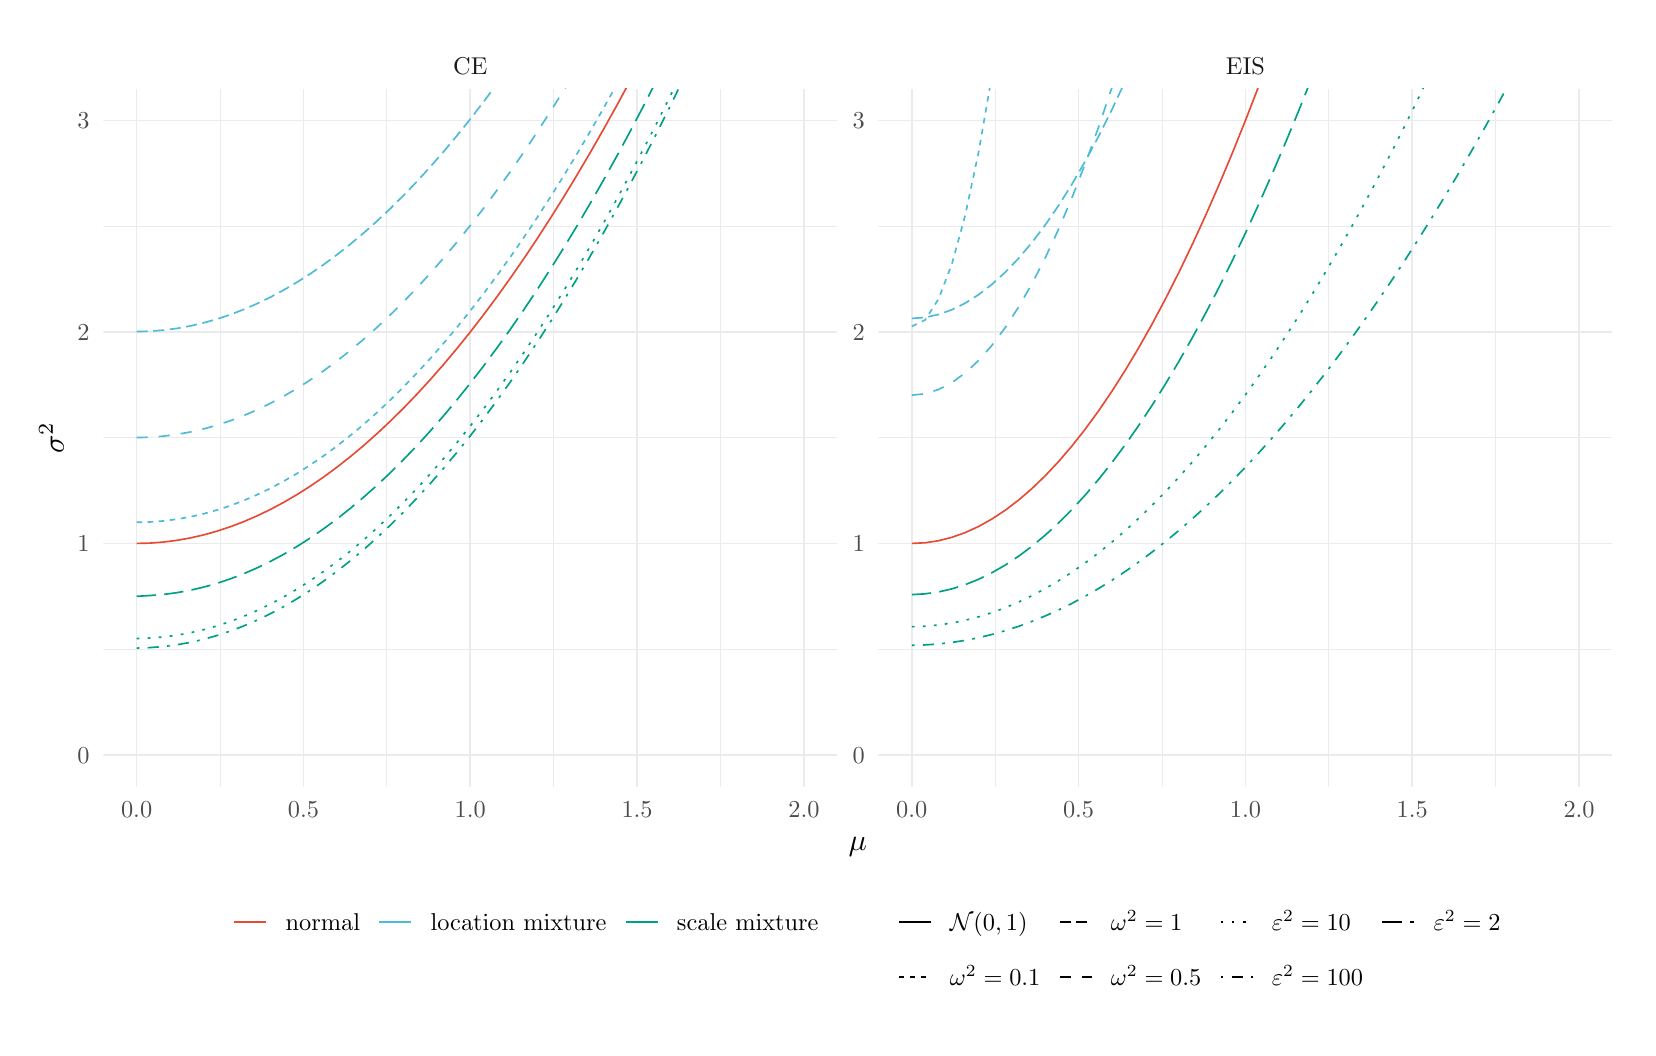
\begin{tikzpicture}[x=1pt,y=1pt]
\definecolor{fillColor}{RGB}{255,255,255}
\path[use as bounding box,fill=fillColor,fill opacity=0.00] (0,0) rectangle (578.16,361.35);
\begin{scope}
\path[clip] ( 27.31, 87.09) rectangle (292.56,339.28);
\definecolor{drawColor}{gray}{0.92}

\path[draw=drawColor,line width= 0.3pt,line join=round] ( 27.31,136.77) --
	(292.56,136.77);

\path[draw=drawColor,line width= 0.3pt,line join=round] ( 27.31,213.19) --
	(292.56,213.19);

\path[draw=drawColor,line width= 0.3pt,line join=round] ( 27.31,289.61) --
	(292.56,289.61);

\path[draw=drawColor,line width= 0.3pt,line join=round] ( 69.51, 87.09) --
	( 69.51,339.28);

\path[draw=drawColor,line width= 0.3pt,line join=round] (129.80, 87.09) --
	(129.80,339.28);

\path[draw=drawColor,line width= 0.3pt,line join=round] (190.08, 87.09) --
	(190.08,339.28);

\path[draw=drawColor,line width= 0.3pt,line join=round] (250.36, 87.09) --
	(250.36,339.28);

\path[draw=drawColor,line width= 0.6pt,line join=round] ( 27.31, 98.56) --
	(292.56, 98.56);

\path[draw=drawColor,line width= 0.6pt,line join=round] ( 27.31,174.98) --
	(292.56,174.98);

\path[draw=drawColor,line width= 0.6pt,line join=round] ( 27.31,251.40) --
	(292.56,251.40);

\path[draw=drawColor,line width= 0.6pt,line join=round] ( 27.31,327.82) --
	(292.56,327.82);

\path[draw=drawColor,line width= 0.6pt,line join=round] ( 39.37, 87.09) --
	( 39.37,339.28);

\path[draw=drawColor,line width= 0.6pt,line join=round] ( 99.65, 87.09) --
	( 99.65,339.28);

\path[draw=drawColor,line width= 0.6pt,line join=round] (159.94, 87.09) --
	(159.94,339.28);

\path[draw=drawColor,line width= 0.6pt,line join=round] (220.22, 87.09) --
	(220.22,339.28);

\path[draw=drawColor,line width= 0.6pt,line join=round] (280.51, 87.09) --
	(280.51,339.28);
\definecolor{drawColor}{RGB}{230,75,53}

\path[draw=drawColor,line width= 0.6pt,line join=round] ( 39.37,174.98) --
	( 44.19,175.10) --
	( 49.02,175.47) --
	( 53.84,176.08) --
	( 58.66,176.93) --
	( 63.48,178.03) --
	( 68.31,179.38) --
	( 73.13,180.97) --
	( 77.95,182.80) --
	( 82.77,184.88) --
	( 87.60,187.20) --
	( 92.42,189.77) --
	( 97.24,192.58) --
	(102.07,195.64) --
	(106.89,198.94) --
	(111.71,202.49) --
	(116.53,206.28) --
	(121.36,210.31) --
	(126.18,214.59) --
	(131.00,219.12) --
	(135.82,223.88) --
	(140.65,228.90) --
	(145.47,234.16) --
	(150.29,239.66) --
	(155.12,245.40) --
	(159.94,251.40) --
	(164.76,257.63) --
	(169.58,264.11) --
	(174.41,270.84) --
	(179.23,277.81) --
	(184.05,285.02) --
	(188.87,292.48) --
	(193.70,300.18) --
	(198.52,308.13) --
	(203.34,316.32) --
	(208.16,324.76) --
	(212.99,333.44) --
	(217.81,342.37) --
	(222.63,351.54) --
	(227.46,360.95) --
	(232.28,370.61) --
	(237.10,380.51) --
	(241.92,390.66) --
	(246.75,401.06) --
	(251.57,411.69) --
	(256.39,422.58) --
	(261.21,433.70) --
	(266.04,445.07) --
	(270.86,456.69) --
	(275.68,468.55) --
	(280.51,480.65);
\definecolor{drawColor}{RGB}{77,187,213}

\path[draw=drawColor,line width= 0.6pt,dash pattern=on 2pt off 2pt ,line join=round] ( 39.37,182.61) --
	( 44.19,182.73) --
	( 49.02,183.10) --
	( 53.84,183.71) --
	( 58.66,184.57) --
	( 63.48,185.67) --
	( 68.31,187.01) --
	( 73.13,188.60) --
	( 77.95,190.44) --
	( 82.77,192.52) --
	( 87.60,194.84) --
	( 92.42,197.41) --
	( 97.24,200.22) --
	(102.07,203.28) --
	(106.89,206.58) --
	(111.71,210.13) --
	(116.53,213.92) --
	(121.36,217.95) --
	(126.18,222.23) --
	(131.00,226.76) --
	(135.82,231.53) --
	(140.65,236.54) --
	(145.47,241.80) --
	(150.29,247.30) --
	(155.12,253.05) --
	(159.94,259.04) --
	(164.76,265.27) --
	(169.58,271.76) --
	(174.41,278.48) --
	(179.23,285.45) --
	(184.05,292.66) --
	(188.87,300.12) --
	(193.70,307.83) --
	(198.52,315.78) --
	(203.34,323.97) --
	(208.16,332.40) --
	(212.99,341.09) --
	(217.81,350.01) --
	(222.63,359.18) --
	(227.46,368.60) --
	(232.28,378.26) --
	(237.10,388.16) --
	(241.92,398.31) --
	(246.75,408.70) --
	(251.57,419.34) --
	(256.39,430.23) --
	(261.21,441.35) --
	(266.04,452.72) --
	(270.86,464.34) --
	(275.68,476.20) --
	(280.51,488.31);

\path[draw=drawColor,line width= 0.6pt,dash pattern=on 4pt off 2pt ,line join=round] ( 39.37,251.53) --
	( 44.19,251.66) --
	( 49.02,252.04) --
	( 53.84,252.67) --
	( 58.66,253.54) --
	( 63.48,254.66) --
	( 68.31,256.02) --
	( 73.13,257.62) --
	( 77.95,259.47) --
	( 82.77,261.57) --
	( 87.60,263.90) --
	( 92.42,266.49) --
	( 97.24,269.31) --
	(102.07,272.39) --
	(106.89,275.70) --
	(111.71,279.26) --
	(116.53,283.07) --
	(121.36,287.12) --
	(126.18,291.41) --
	(131.00,295.95) --
	(135.82,300.74) --
	(140.65,305.76) --
	(145.47,311.04) --
	(150.29,316.55) --
	(155.12,322.32) --
	(159.94,328.32) --
	(164.76,334.57) --
	(169.58,341.07) --
	(174.41,347.81) --
	(179.23,354.79) --
	(184.05,362.02) --
	(188.87,369.50) --
	(193.70,377.22) --
	(198.52,385.18) --
	(203.34,393.39) --
	(208.16,401.84) --
	(212.99,410.53) --
	(217.81,419.47) --
	(222.63,428.66) --
	(227.46,438.09) --
	(232.28,447.76) --
	(237.10,457.68) --
	(241.92,467.85) --
	(246.75,478.26) --
	(251.57,488.91) --
	(256.39,499.81) --
	(261.21,510.95) --
	(266.04,522.33) --
	(270.86,533.96) --
	(275.68,545.84) --
	(280.51,557.96);

\path[draw=drawColor,line width= 0.6pt,dash pattern=on 4pt off 4pt ,line join=round] ( 39.37,213.23) --
	( 44.19,213.36) --
	( 49.02,213.74) --
	( 53.84,214.36) --
	( 58.66,215.22) --
	( 63.48,216.33) --
	( 68.31,217.68) --
	( 73.13,219.28) --
	( 77.95,221.13) --
	( 82.77,223.21) --
	( 87.60,225.55) --
	( 92.42,228.12) --
	( 97.24,230.94) --
	(102.07,234.01) --
	(106.89,237.32) --
	(111.71,240.87) --
	(116.53,244.67) --
	(121.36,248.72) --
	(126.18,253.00) --
	(131.00,257.54) --
	(135.82,262.31) --
	(140.65,267.34) --
	(145.47,272.60) --
	(150.29,278.11) --
	(155.12,283.87) --
	(159.94,289.87) --
	(164.76,296.11) --
	(169.58,302.60) --
	(174.41,309.34) --
	(179.23,316.32) --
	(184.05,323.54) --
	(188.87,331.01) --
	(193.70,338.72) --
	(198.52,346.67) --
	(203.34,354.88) --
	(208.16,363.32) --
	(212.99,372.01) --
	(217.81,380.95) --
	(222.63,390.12) --
	(227.46,399.55) --
	(232.28,409.22) --
	(237.10,419.13) --
	(241.92,429.29) --
	(246.75,439.69) --
	(251.57,450.33) --
	(256.39,461.23) --
	(261.21,472.36) --
	(266.04,483.74) --
	(270.86,495.37) --
	(275.68,507.24) --
	(280.51,519.35);
\definecolor{drawColor}{RGB}{0,160,135}

\path[draw=drawColor,line width= 0.6pt,dash pattern=on 1pt off 3pt ,line join=round] ( 39.37,140.59) --
	( 44.19,140.80) --
	( 49.02,141.18) --
	( 53.84,141.80) --
	( 58.66,142.67) --
	( 63.48,143.78) --
	( 68.31,145.14) --
	( 73.13,146.74) --
	( 77.95,148.59) --
	( 82.77,150.68) --
	( 87.60,153.02) --
	( 92.42,155.60) --
	( 97.24,158.42) --
	(102.07,161.49) --
	(106.89,164.81) --
	(111.71,168.36) --
	(116.53,172.17) --
	(121.36,176.22) --
	(126.18,180.51) --
	(131.00,185.05) --
	(135.82,189.83) --
	(140.65,194.85) --
	(145.47,200.12) --
	(150.29,205.64) --
	(155.12,211.40) --
	(159.94,217.40) --
	(164.76,223.65) --
	(169.58,230.14) --
	(174.41,236.88) --
	(179.23,243.86) --
	(184.05,251.09) --
	(188.87,258.56) --
	(193.70,266.28) --
	(198.52,274.24) --
	(203.34,282.44) --
	(208.16,290.89) --
	(212.99,299.59) --
	(217.81,308.53) --
	(222.63,317.71) --
	(227.46,327.14) --
	(232.28,336.81) --
	(237.10,346.73) --
	(241.92,356.89) --
	(246.75,367.29) --
	(251.57,377.94) --
	(256.39,388.84) --
	(261.21,399.98) --
	(266.04,411.36) --
	(270.86,422.99) --
	(275.68,434.86) --
	(280.51,446.98);

\path[draw=drawColor,line width= 0.6pt,dash pattern=on 1pt off 3pt on 4pt off 3pt ,line join=round] ( 39.37,137.15) --
	( 44.19,137.34) --
	( 49.02,137.72) --
	( 53.84,138.34) --
	( 58.66,139.20) --
	( 63.48,140.31) --
	( 68.31,141.67) --
	( 73.13,143.27) --
	( 77.95,145.11) --
	( 82.77,147.20) --
	( 87.60,149.53) --
	( 92.42,152.11) --
	( 97.24,154.93) --
	(102.07,158.00) --
	(106.89,161.31) --
	(111.71,164.87) --
	(116.53,168.67) --
	(121.36,172.71) --
	(126.18,177.00) --
	(131.00,181.54) --
	(135.82,186.32) --
	(140.65,191.34) --
	(145.47,196.61) --
	(150.29,202.12) --
	(155.12,207.88) --
	(159.94,213.88) --
	(164.76,220.12) --
	(169.58,226.62) --
	(174.41,233.35) --
	(179.23,240.33) --
	(184.05,247.55) --
	(188.87,255.02) --
	(193.70,262.74) --
	(198.52,270.69) --
	(203.34,278.90) --
	(208.16,287.34) --
	(212.99,296.03) --
	(217.81,304.97) --
	(222.63,314.15) --
	(227.46,323.58) --
	(232.28,333.24) --
	(237.10,343.16) --
	(241.92,353.32) --
	(246.75,363.72) --
	(251.57,374.37) --
	(256.39,385.26) --
	(261.21,396.40) --
	(266.04,407.78) --
	(270.86,419.40) --
	(275.68,431.28) --
	(280.51,443.39);

\path[draw=drawColor,line width= 0.6pt,dash pattern=on 7pt off 3pt ,line join=round] ( 39.37,155.87) --
	( 44.19,156.15) --
	( 49.02,156.54) --
	( 53.84,157.17) --
	( 58.66,158.04) --
	( 63.48,159.16) --
	( 68.31,160.52) --
	( 73.13,162.13) --
	( 77.95,163.98) --
	( 82.77,166.08) --
	( 87.60,168.42) --
	( 92.42,171.00) --
	( 97.24,173.83) --
	(102.07,176.91) --
	(106.89,180.23) --
	(111.71,183.79) --
	(116.53,187.60) --
	(121.36,191.65) --
	(126.18,195.95) --
	(131.00,200.49) --
	(135.82,205.28) --
	(140.65,210.31) --
	(145.47,215.59) --
	(150.29,221.11) --
	(155.12,226.87) --
	(159.94,232.88) --
	(164.76,239.13) --
	(169.58,245.63) --
	(174.41,252.37) --
	(179.23,259.36) --
	(184.05,266.59) --
	(188.87,274.07) --
	(193.70,281.79) --
	(198.52,289.76) --
	(203.34,297.97) --
	(208.16,306.42) --
	(212.99,315.12) --
	(217.81,324.06) --
	(222.63,333.25) --
	(227.46,342.69) --
	(232.28,352.36) --
	(237.10,362.28) --
	(241.92,372.45) --
	(246.75,382.86) --
	(251.57,393.52) --
	(256.39,404.42) --
	(261.21,415.56) --
	(266.04,426.95) --
	(270.86,438.58) --
	(275.68,450.46) --
	(280.51,462.59);
\end{scope}
\begin{scope}
\path[clip] (307.41, 87.09) rectangle (572.66,339.28);
\definecolor{drawColor}{gray}{0.92}

\path[draw=drawColor,line width= 0.3pt,line join=round] (307.41,136.77) --
	(572.66,136.77);

\path[draw=drawColor,line width= 0.3pt,line join=round] (307.41,213.19) --
	(572.66,213.19);

\path[draw=drawColor,line width= 0.3pt,line join=round] (307.41,289.61) --
	(572.66,289.61);

\path[draw=drawColor,line width= 0.3pt,line join=round] (349.61, 87.09) --
	(349.61,339.28);

\path[draw=drawColor,line width= 0.3pt,line join=round] (409.89, 87.09) --
	(409.89,339.28);

\path[draw=drawColor,line width= 0.3pt,line join=round] (470.18, 87.09) --
	(470.18,339.28);

\path[draw=drawColor,line width= 0.3pt,line join=round] (530.46, 87.09) --
	(530.46,339.28);

\path[draw=drawColor,line width= 0.6pt,line join=round] (307.41, 98.56) --
	(572.66, 98.56);

\path[draw=drawColor,line width= 0.6pt,line join=round] (307.41,174.98) --
	(572.66,174.98);

\path[draw=drawColor,line width= 0.6pt,line join=round] (307.41,251.40) --
	(572.66,251.40);

\path[draw=drawColor,line width= 0.6pt,line join=round] (307.41,327.82) --
	(572.66,327.82);

\path[draw=drawColor,line width= 0.6pt,line join=round] (319.47, 87.09) --
	(319.47,339.28);

\path[draw=drawColor,line width= 0.6pt,line join=round] (379.75, 87.09) --
	(379.75,339.28);

\path[draw=drawColor,line width= 0.6pt,line join=round] (440.04, 87.09) --
	(440.04,339.28);

\path[draw=drawColor,line width= 0.6pt,line join=round] (500.32, 87.09) --
	(500.32,339.28);

\path[draw=drawColor,line width= 0.6pt,line join=round] (560.60, 87.09) --
	(560.60,339.28);
\definecolor{drawColor}{RGB}{230,75,53}

\path[draw=drawColor,line width= 0.6pt,line join=round] (319.47,174.98) --
	(324.29,175.22) --
	(329.11,175.95) --
	(333.94,177.18) --
	(338.76,178.89) --
	(343.58,181.09) --
	(348.40,183.78) --
	(353.23,186.96) --
	(358.05,190.63) --
	(362.87,194.78) --
	(367.69,199.43) --
	(372.52,204.57) --
	(377.34,210.19) --
	(382.16,216.30) --
	(386.99,222.91) --
	(391.81,230.00) --
	(396.63,237.58) --
	(401.45,245.65) --
	(406.28,254.21) --
	(411.10,263.26) --
	(415.92,272.79) --
	(420.74,282.82) --
	(425.57,293.34) --
	(430.39,304.34) --
	(435.21,315.83) --
	(440.04,327.82) --
	(444.86,340.29) --
	(449.68,353.25) --
	(454.50,366.70) --
	(459.33,380.64) --
	(464.15,395.06) --
	(468.97,409.98) --
	(473.79,425.39) --
	(478.62,441.28) --
	(483.44,457.67) --
	(488.26,474.54) --
	(493.09,491.90) --
	(497.91,509.76) --
	(502.73,528.10) --
	(507.55,546.93) --
	(512.38,566.24) --
	(517.20,586.05) --
	(522.02,606.35) --
	(526.84,627.14) --
	(531.67,648.41) --
	(536.49,670.18) --
	(541.31,692.43) --
	(546.14,715.17) --
	(550.96,738.40) --
	(555.78,762.12) --
	(560.60,786.33);
\definecolor{drawColor}{RGB}{77,187,213}

\path[draw=drawColor,line width= 0.6pt,dash pattern=on 2pt off 2pt ,line join=round] (319.47,253.37) --
	(324.29,255.74) --
	(329.11,263.25) --
	(333.94,275.85) --
	(338.76,293.50) --
	(343.58,316.21) --
	(348.40,343.89) --
	(353.23,376.55) --
	(358.05,414.12) --
	(362.87,456.58) --
	(367.69,503.89) --
	(372.52,556.02) --
	(377.34,612.95) --
	(382.16,674.67) --
	(386.99,741.02) --
	(391.81,812.14) --
	(396.63,887.86) --
	(401.45,968.22) --
	(406.28,1053.15) --
	(411.10,1142.72) --
	(415.92,1236.78) --
	(420.74,1335.35) --
	(425.57,1438.31) --
	(430.39,1545.87) --
	(435.21,1657.71) --
	(440.04,1773.94) --
	(444.86,1894.45) --
	(449.68,2019.33) --
	(454.50,2149.01) --
	(459.33,2282.57) --
	(464.15,2420.09) --
	(468.97,2562.24) --
	(472.67,2673.99);

\path[draw=drawColor,line width= 0.6pt,dash pattern=on 4pt off 2pt ,line join=round] (319.47,256.27) --
	(324.29,256.65) --
	(329.11,257.70) --
	(333.94,259.42) --
	(338.76,261.80) --
	(343.58,264.85) --
	(348.40,268.56) --
	(353.23,272.94) --
	(358.05,277.98) --
	(362.87,283.68) --
	(367.69,290.05) --
	(372.52,297.08) --
	(377.34,304.77) --
	(382.16,313.11) --
	(386.99,322.12) --
	(391.81,331.79) --
	(396.63,342.12) --
	(401.45,353.10) --
	(406.28,364.74) --
	(411.10,377.04) --
	(415.92,389.99) --
	(420.74,403.59) --
	(425.57,417.85) --
	(430.39,432.76) --
	(435.21,448.32) --
	(440.04,464.53) --
	(444.86,481.40) --
	(449.68,498.91) --
	(454.50,517.07) --
	(459.33,535.88) --
	(464.15,555.33) --
	(468.97,575.44) --
	(473.79,596.19) --
	(478.62,617.61) --
	(483.44,639.64) --
	(488.26,662.32) --
	(493.09,685.68) --
	(497.91,709.64) --
	(502.73,734.25) --
	(507.55,759.50) --
	(512.38,785.43) --
	(517.20,811.96) --
	(522.02,839.13) --
	(526.84,866.96) --
	(531.67,895.44) --
	(536.49,924.52) --
	(541.31,954.24) --
	(546.14,984.62) --
	(550.96,1015.61) --
	(555.78,1047.23) --
	(560.60,1079.50);

\path[draw=drawColor,line width= 0.6pt,dash pattern=on 4pt off 4pt ,line join=round] (319.47,228.55) --
	(324.29,229.07) --
	(329.11,230.58) --
	(333.94,233.08) --
	(338.76,236.57) --
	(343.58,241.05) --
	(348.40,246.51) --
	(353.23,252.95) --
	(358.05,260.38) --
	(362.87,268.79) --
	(367.69,278.18) --
	(372.52,288.55) --
	(377.34,299.89) --
	(382.16,312.21) --
	(386.99,325.51) --
	(391.81,339.77) --
	(396.63,355.01) --
	(401.45,371.21) --
	(406.28,388.38) --
	(411.10,406.52) --
	(415.92,425.62) --
	(420.74,445.70) --
	(425.57,466.71) --
	(430.39,488.70) --
	(435.21,511.65) --
	(440.04,535.55) --
	(444.86,560.41) --
	(449.68,586.21) --
	(454.50,612.97) --
	(459.33,640.69) --
	(464.15,669.32) --
	(468.97,699.01) --
	(473.79,729.54) --
	(478.62,761.07) --
	(483.44,793.48) --
	(488.26,826.91) --
	(493.09,861.17) --
	(497.91,896.51) --
	(502.73,932.63) --
	(507.55,969.87) --
	(512.38,1007.97) --
	(517.20,1046.99) --
	(522.02,1086.95) --
	(526.84,1127.81) --
	(531.67,1169.63) --
	(536.49,1212.38) --
	(541.31,1256.07) --
	(546.14,1300.60) --
	(550.96,1346.15) --
	(555.78,1392.61) --
	(560.60,1440.03);
\definecolor{drawColor}{RGB}{0,160,135}

\path[draw=drawColor,line width= 0.6pt,dash pattern=on 1pt off 3pt ,line join=round] (319.47,144.89) --
	(324.29,145.06) --
	(329.11,145.51) --
	(333.94,146.22) --
	(338.76,147.20) --
	(343.58,148.44) --
	(348.40,149.96) --
	(353.23,151.73) --
	(358.05,153.78) --
	(362.87,156.09) --
	(367.69,158.66) --
	(372.52,161.50) --
	(377.34,164.60) --
	(382.16,167.97) --
	(386.99,171.59) --
	(391.81,175.48) --
	(396.63,179.63) --
	(401.45,184.05) --
	(406.28,188.72) --
	(411.10,193.65) --
	(415.92,198.85) --
	(420.74,204.30) --
	(425.57,210.01) --
	(430.39,215.98) --
	(435.21,222.21) --
	(440.04,228.70) --
	(444.86,235.44) --
	(449.68,242.44) --
	(454.50,249.70) --
	(459.33,257.21) --
	(464.15,264.98) --
	(468.97,273.00) --
	(473.79,281.28) --
	(478.62,289.81) --
	(483.44,298.59) --
	(488.26,307.63) --
	(493.09,316.92) --
	(497.91,326.46) --
	(502.73,336.26) --
	(507.55,346.30) --
	(512.38,356.60) --
	(517.20,367.15) --
	(522.02,377.95) --
	(526.84,388.99) --
	(531.67,400.29) --
	(536.49,411.84) --
	(541.31,423.63) --
	(546.14,435.67) --
	(550.96,447.94) --
	(555.78,460.49) --
	(560.60,473.29);

\path[draw=drawColor,line width= 0.6pt,dash pattern=on 1pt off 3pt on 4pt off 3pt ,line join=round] (319.47,138.17) --
	(324.29,138.31) --
	(329.11,138.65) --
	(333.94,139.20) --
	(338.76,139.95) --
	(343.58,140.91) --
	(348.40,142.07) --
	(353.23,143.44) --
	(358.05,145.01) --
	(362.87,146.79) --
	(367.69,148.77) --
	(372.52,150.94) --
	(377.34,153.32) --
	(382.16,155.91) --
	(386.99,158.69) --
	(391.81,161.68) --
	(396.63,164.86) --
	(401.45,168.25) --
	(406.28,171.84) --
	(411.10,175.62) --
	(415.92,179.61) --
	(420.74,183.80) --
	(425.57,188.18) --
	(430.39,192.77) --
	(435.21,197.55) --
	(440.04,202.53) --
	(444.86,207.71) --
	(449.68,213.09) --
	(454.50,218.66) --
	(459.33,224.43) --
	(464.15,230.41) --
	(468.97,236.57) --
	(473.79,242.93) --
	(478.62,249.49) --
	(483.44,256.25) --
	(488.26,263.19) --
	(493.09,270.33) --
	(497.91,277.68) --
	(502.73,285.21) --
	(507.55,292.94) --
	(512.38,300.86) --
	(517.20,308.97) --
	(522.02,317.29) --
	(526.84,325.79) --
	(531.67,334.49) --
	(536.49,343.38) --
	(541.31,352.45) --
	(546.14,361.73) --
	(550.96,371.19) --
	(555.78,380.85) --
	(560.60,390.70);

\path[draw=drawColor,line width= 0.6pt,dash pattern=on 7pt off 3pt ,line join=round] (319.47,156.49) --
	(324.29,156.76) --
	(329.11,157.44) --
	(333.94,158.55) --
	(338.76,160.07) --
	(343.58,162.02) --
	(348.40,164.38) --
	(353.23,167.15) --
	(358.05,170.34) --
	(362.87,173.95) --
	(367.69,177.96) --
	(372.52,182.39) --
	(377.34,187.23) --
	(382.16,192.48) --
	(386.99,198.14) --
	(391.81,204.21) --
	(396.63,210.68) --
	(401.45,217.56) --
	(406.28,224.85) --
	(411.10,232.54) --
	(415.92,240.63) --
	(420.74,249.13) --
	(425.57,258.02) --
	(430.39,267.32) --
	(435.21,277.01) --
	(440.04,287.11) --
	(444.86,297.60) --
	(449.68,308.49) --
	(454.50,319.77) --
	(459.33,331.45) --
	(464.15,343.52) --
	(468.97,355.99) --
	(473.79,368.84) --
	(478.62,382.09) --
	(483.44,395.73) --
	(488.26,409.75) --
	(493.09,424.17) --
	(497.91,438.97) --
	(502.73,454.15) --
	(507.55,469.73) --
	(512.38,485.70) --
	(517.20,502.03) --
	(522.02,518.76) --
	(526.84,535.86) --
	(531.67,553.34) --
	(536.49,571.22) --
	(541.31,589.48) --
	(546.14,608.07) --
	(550.96,627.10) --
	(555.78,646.47) --
	(560.60,666.22);
\end{scope}
\begin{scope}
\path[clip] ( 27.31,339.28) rectangle (292.56,355.85);
\definecolor{drawColor}{gray}{0.10}

\node[text=drawColor,anchor=base,inner sep=0pt, outer sep=0pt, scale=  0.88] at (159.94,344.53) {CE};
\end{scope}
\begin{scope}
\path[clip] (307.41,339.28) rectangle (572.66,355.85);
\definecolor{drawColor}{gray}{0.10}

\node[text=drawColor,anchor=base,inner sep=0pt, outer sep=0pt, scale=  0.88] at (440.04,344.53) {EIS};
\end{scope}
\begin{scope}
\path[clip] (  0.00,  0.00) rectangle (578.16,361.35);
\definecolor{drawColor}{gray}{0.30}

\node[text=drawColor,anchor=base,inner sep=0pt, outer sep=0pt, scale=  0.88] at ( 39.37, 76.08) {0.0};

\node[text=drawColor,anchor=base,inner sep=0pt, outer sep=0pt, scale=  0.88] at ( 99.65, 76.08) {0.5};

\node[text=drawColor,anchor=base,inner sep=0pt, outer sep=0pt, scale=  0.88] at (159.94, 76.08) {1.0};

\node[text=drawColor,anchor=base,inner sep=0pt, outer sep=0pt, scale=  0.88] at (220.22, 76.08) {1.5};

\node[text=drawColor,anchor=base,inner sep=0pt, outer sep=0pt, scale=  0.88] at (280.51, 76.08) {2.0};
\end{scope}
\begin{scope}
\path[clip] (  0.00,  0.00) rectangle (578.16,361.35);
\definecolor{drawColor}{gray}{0.30}

\node[text=drawColor,anchor=base,inner sep=0pt, outer sep=0pt, scale=  0.88] at (319.47, 76.08) {0.0};

\node[text=drawColor,anchor=base,inner sep=0pt, outer sep=0pt, scale=  0.88] at (379.75, 76.08) {0.5};

\node[text=drawColor,anchor=base,inner sep=0pt, outer sep=0pt, scale=  0.88] at (440.04, 76.08) {1.0};

\node[text=drawColor,anchor=base,inner sep=0pt, outer sep=0pt, scale=  0.88] at (500.32, 76.08) {1.5};

\node[text=drawColor,anchor=base,inner sep=0pt, outer sep=0pt, scale=  0.88] at (560.60, 76.08) {2.0};
\end{scope}
\begin{scope}
\path[clip] (  0.00,  0.00) rectangle (578.16,361.35);
\definecolor{drawColor}{gray}{0.30}

\node[text=drawColor,anchor=base east,inner sep=0pt, outer sep=0pt, scale=  0.88] at (302.46, 95.53) {0};

\node[text=drawColor,anchor=base east,inner sep=0pt, outer sep=0pt, scale=  0.88] at (302.46,171.95) {1};

\node[text=drawColor,anchor=base east,inner sep=0pt, outer sep=0pt, scale=  0.88] at (302.46,248.37) {2};

\node[text=drawColor,anchor=base east,inner sep=0pt, outer sep=0pt, scale=  0.88] at (302.46,324.79) {3};
\end{scope}
\begin{scope}
\path[clip] (  0.00,  0.00) rectangle (578.16,361.35);
\definecolor{drawColor}{gray}{0.30}

\node[text=drawColor,anchor=base east,inner sep=0pt, outer sep=0pt, scale=  0.88] at ( 22.36, 95.53) {0};

\node[text=drawColor,anchor=base east,inner sep=0pt, outer sep=0pt, scale=  0.88] at ( 22.36,171.95) {1};

\node[text=drawColor,anchor=base east,inner sep=0pt, outer sep=0pt, scale=  0.88] at ( 22.36,248.37) {2};

\node[text=drawColor,anchor=base east,inner sep=0pt, outer sep=0pt, scale=  0.88] at ( 22.36,324.79) {3};
\end{scope}
\begin{scope}
\path[clip] (  0.00,  0.00) rectangle (578.16,361.35);
\definecolor{drawColor}{RGB}{0,0,0}

\node[text=drawColor,anchor=base,inner sep=0pt, outer sep=0pt, scale=  1.10] at (299.99, 64.05) {$\mu$};
\end{scope}
\begin{scope}
\path[clip] (  0.00,  0.00) rectangle (578.16,361.35);
\definecolor{drawColor}{RGB}{0,0,0}

\node[text=drawColor,rotate= 90.00,anchor=base,inner sep=0pt, outer sep=0pt, scale=  1.10] at ( 13.08,213.19) {$\sigma^2$};
\end{scope}
\begin{scope}
\path[clip] (  0.00,  0.00) rectangle (578.16,361.35);
\definecolor{drawColor}{RGB}{230,75,53}

\path[draw=drawColor,line width= 0.6pt,line join=round] ( 74.73, 38.18) -- ( 86.29, 38.18);
\end{scope}
\begin{scope}
\path[clip] (  0.00,  0.00) rectangle (578.16,361.35);
\definecolor{drawColor}{RGB}{77,187,213}

\path[draw=drawColor,line width= 0.6pt,line join=round] (127.09, 38.18) -- (138.65, 38.18);
\end{scope}
\begin{scope}
\path[clip] (  0.00,  0.00) rectangle (578.16,361.35);
\definecolor{drawColor}{RGB}{0,160,135}

\path[draw=drawColor,line width= 0.6pt,line join=round] (216.11, 38.18) -- (227.67, 38.18);
\end{scope}
\begin{scope}
\path[clip] (  0.00,  0.00) rectangle (578.16,361.35);
\definecolor{drawColor}{RGB}{0,0,0}

\node[text=drawColor,anchor=base west,inner sep=0pt, outer sep=0pt, scale=  0.88] at ( 93.24, 35.15) {normal};
\end{scope}
\begin{scope}
\path[clip] (  0.00,  0.00) rectangle (578.16,361.35);
\definecolor{drawColor}{RGB}{0,0,0}

\node[text=drawColor,anchor=base west,inner sep=0pt, outer sep=0pt, scale=  0.88] at (145.60, 35.15) {location mixture};
\end{scope}
\begin{scope}
\path[clip] (  0.00,  0.00) rectangle (578.16,361.35);
\definecolor{drawColor}{RGB}{0,0,0}

\node[text=drawColor,anchor=base west,inner sep=0pt, outer sep=0pt, scale=  0.88] at (234.62, 35.15) {scale mixture};
\end{scope}
\begin{scope}
\path[clip] (  0.00,  0.00) rectangle (578.16,361.35);
\definecolor{drawColor}{RGB}{0,0,0}

\path[draw=drawColor,line width= 0.6pt,line join=round] (314.71, 38.18) -- (326.28, 38.18);
\end{scope}
\begin{scope}
\path[clip] (  0.00,  0.00) rectangle (578.16,361.35);
\definecolor{drawColor}{RGB}{0,0,0}

\path[draw=drawColor,line width= 0.6pt,dash pattern=on 2pt off 2pt ,line join=round] (314.71, 18.23) -- (326.28, 18.23);
\end{scope}
\begin{scope}
\path[clip] (  0.00,  0.00) rectangle (578.16,361.35);
\definecolor{drawColor}{RGB}{0,0,0}

\path[draw=drawColor,line width= 0.6pt,dash pattern=on 4pt off 2pt ,line join=round] (372.89, 38.18) -- (384.45, 38.18);
\end{scope}
\begin{scope}
\path[clip] (  0.00,  0.00) rectangle (578.16,361.35);
\definecolor{drawColor}{RGB}{0,0,0}

\path[draw=drawColor,line width= 0.6pt,dash pattern=on 4pt off 4pt ,line join=round] (372.89, 18.23) -- (384.45, 18.23);
\end{scope}
\begin{scope}
\path[clip] (  0.00,  0.00) rectangle (578.16,361.35);
\definecolor{drawColor}{RGB}{0,0,0}

\path[draw=drawColor,line width= 0.6pt,dash pattern=on 1pt off 3pt ,line join=round] (431.06, 38.18) -- (442.62, 38.18);
\end{scope}
\begin{scope}
\path[clip] (  0.00,  0.00) rectangle (578.16,361.35);
\definecolor{drawColor}{RGB}{0,0,0}

\path[draw=drawColor,line width= 0.6pt,dash pattern=on 1pt off 3pt on 4pt off 3pt ,line join=round] (431.06, 18.23) -- (442.62, 18.23);
\end{scope}
\begin{scope}
\path[clip] (  0.00,  0.00) rectangle (578.16,361.35);
\definecolor{drawColor}{RGB}{0,0,0}

\path[draw=drawColor,line width= 0.6pt,dash pattern=on 7pt off 3pt ,line join=round] (489.50, 38.18) -- (501.06, 38.18);
\end{scope}
\begin{scope}
\path[clip] (  0.00,  0.00) rectangle (578.16,361.35);
\definecolor{drawColor}{RGB}{0,0,0}

\node[text=drawColor,anchor=base west,inner sep=0pt, outer sep=0pt, scale=  0.88] at (333.22, 35.15) {$\mathcal N (0, 1)$};
\end{scope}
\begin{scope}
\path[clip] (  0.00,  0.00) rectangle (578.16,361.35);
\definecolor{drawColor}{RGB}{0,0,0}

\node[text=drawColor,anchor=base west,inner sep=0pt, outer sep=0pt, scale=  0.88] at (333.22, 15.20) {$\omega^2 = 0.1$};
\end{scope}
\begin{scope}
\path[clip] (  0.00,  0.00) rectangle (578.16,361.35);
\definecolor{drawColor}{RGB}{0,0,0}

\node[text=drawColor,anchor=base west,inner sep=0pt, outer sep=0pt, scale=  0.88] at (391.39, 35.15) {$\omega^2 = 1$};
\end{scope}
\begin{scope}
\path[clip] (  0.00,  0.00) rectangle (578.16,361.35);
\definecolor{drawColor}{RGB}{0,0,0}

\node[text=drawColor,anchor=base west,inner sep=0pt, outer sep=0pt, scale=  0.88] at (391.39, 15.20) {$\omega^2= 0.5$};
\end{scope}
\begin{scope}
\path[clip] (  0.00,  0.00) rectangle (578.16,361.35);
\definecolor{drawColor}{RGB}{0,0,0}

\node[text=drawColor,anchor=base west,inner sep=0pt, outer sep=0pt, scale=  0.88] at (449.57, 35.15) {$\varepsilon^2 = 10$};
\end{scope}
\begin{scope}
\path[clip] (  0.00,  0.00) rectangle (578.16,361.35);
\definecolor{drawColor}{RGB}{0,0,0}

\node[text=drawColor,anchor=base west,inner sep=0pt, outer sep=0pt, scale=  0.88] at (449.57, 15.20) {$\varepsilon^2 = 100$};
\end{scope}
\begin{scope}
\path[clip] (  0.00,  0.00) rectangle (578.16,361.35);
\definecolor{drawColor}{RGB}{0,0,0}

\node[text=drawColor,anchor=base west,inner sep=0pt, outer sep=0pt, scale=  0.88] at (508.01, 35.15) {$\varepsilon^2 = 2$};
\end{scope}
\end{tikzpicture}
%
    }
    \caption{{\color{red} TODO}}
    \label{fig:cem_eis_sigma2}
\end{figure}

% AREs
On the left-hand side of \Cref{fig:are} we see that for $\mu$ close to the optimal value, \aeis has smaller asymptotic variance than the \acem, except for the two bimodal location measures. Again, due to the finite sample convergence of \aeis, \Cref{prop:eis-finite-sample}, the asymptotic variance $V_{\eis}$ goes to $0$ as $\mu \to 0$. The more $\mu$ becomes misspecified, the ratio of asymptotic variances starts to grow. 

% sigma2s
In \Cref{fig:cem_eis_sigma2} we see that, except for the extreme scale mixtures, \aeis tends to produce proposals that have a larger variance than those produced by the \acem. As we will see in the discussion of \Cref{fig:rho_mu}, this might be advantageous for \aeis as proposals with a small variance run the risk of missing a large part of the probability mass of the target. \todo{clean this}

In applications, e.g. the model studied in \Cref{cha:analysis_of_selected_models}, we are interested in the performance of the importance sampling proposals generated by the \gls{la}, \gls{cem} and \gls{eis} under more complex circumstances than those discussed in \Cref{ex:univ-gaussian-mu-fixed,ex:univ-gaussian-s2-fixed}. In particular, the dimension of $\psi$ is high ($\mathcal O(n \cdot m)$ or even $\mathcal O(n \cdot m^{2})$) and proposals may not come from a natural exponential family, so analysis based on \Cref{thm:ce-clt,thm:clt-eis} is not possible. Instead, we resort to simulation studies to gain insights into the circumstances when one should prefer one method over the other.
As a leading example, we will use the following vector-autoregressive state space model with negative binomial observations. A similar, though more involved, model is studied in \Cref{sec:regional_growth_factor_model} with real data.

\begin{example}[Negative Binomial $\operatorname{VAR}(1)$ \gls{ssm}]
    \label{ex:negbinom-ar1}
    % setup 
    In this example, we consider a \gls{ssm} where states $X_{t}$ follow a stationary Gaussian $\operatorname{VAR}(1)$ process, initialized in its stationary distribution $\mathcal N(0,\Sigma)$ for \acrshort{spd} $\Sigma$. For simplicity let the transition matrices be given by a multiple of the identity, i.e. $A_{t} = \alpha I_{m}$ for all $t$ where $\alpha \in (-1, 1)$ \todo{add I to symbols}. 
    In total, the states are governed by
    \begin{align*}
    X_{0} &\sim \mathcal N(0,\Sigma) \\
    X_{t} &= \alpha X_{t - 1} + \varepsilon_{t}\\
    \varepsilon_t &\iid \mathcal N(0, (1 - \alpha^{2})\Sigma), t = 1, \dots, n
    \end{align*}
    where the $\varepsilon_{1}, \dots, n$ and $X_{0}$ are jointly independent. The observations follow a conditional negative binomial distribution 
    $$
    Y^{i}_{t} | X_{t} \sim \nbinom \left( \exp(X^{i}_{t}), r \right), \phantom{and} i = 1, \dots, p \phantom{and} t = 0, \dots, n
    $$
    and individual observations are conditionally independent given the current state. The parametrization of the negative binomial distribution $\nbinom \left( \mu, r \right)$ is such that the density is
    $$
        p_{\mu, r}(y) = \binom{y + r - 1}{r} \left( \frac{\mu}{r + \mu} \right)^{y} \left( \frac{r}{r + \mu} \right)^{r} \propto_{\mu} \mu^{y} (\mu + r)^{-(r + y)},
    $$
    with expectation $\mu$, variance $\mu + \frac{\mu^{2}}{r}$ and support $\N_{0}$. 
\end{example}

%% simulation study on MSE/Bias/Variance

Our first simulation study concerns the non-asymptotic behavior of the \gls{cem} and \gls{eis} estimators, i.e. finite sample analogs of \Cref{thm:ce-clt,thm:clt-eis}. To this end,
we let $m = 1$ in \Cref{ex:negbinom-ar1} and fix $n$ to \todo{...}. 
We then simulate once from the marginal distribution of $Y$ and perform the \gls{la} to a prespecified precision $\epsilon$ and maximum number of iterations $n_{\text{iter}}$, obtaining a proposal distribution $\G_{\la}$. Using a large number of samples $N_{\text{true}}$ from this proposal we find the optimal $\G_{\ce}$ and $\G_{\eis}$ using the same desired precision and number of iterations as for the \gls{la}. For the remainder of this section, we ignore sampling variation in these proposals and treat them as exact. 

%% posterior marginal means and variances
To determine the non-asymptotic sampling behavior we now perform the above procedure again, using only $N \ll N_{\text{true}}$ many samples for both procedures, obtaining proposals $\hat\P^{N}_{\ce}$ and $\hat \P^{N}_{\eis}$. As the full proposals are Gaussian distributions on $\R^{(n+1)\times m}$, either given as the posterior of a \gls{glssm} (\gls{la}, \gls{eis}) or by a Gaussian Markov process(\gls{cem}), see \Cref{sec:gaussian_importance_sampling_for_state_space_models}. 
This procedure is repeated $M$ times for every sample size $N$ considered, with different initial random seeds, obtaining $\hat\P^{N,i}_{\ce}$ and $\hat \P^{N,i}_{\eis}$ for $i = 1, \dots, M$.

To assess the speed of convergence of the \gls{cem} and \gls{eis} we then estimate the mean squared error of means and variances of the $(n+1) \times m$ univariate marginals as $N$, the number of samples used to obtain $\hpce$ or $\hpeis$, grows. For the true value, we take the univariate means and variances of $\G_{\ce}$ and $\G_{\eis}$ respectively. Additionally, we perform a bias-variance decomposition to see where the estimation error originates. 

More concretely, fix $N$ and denote by $\mu, \sigma^{2} \in \mathbf R^{(n + 1) \cdot m}$ the marginal means and variances of $\G_{\ce}$ ($\G_{\eis}$). 
Let $\hat\mu_{i}, \hat\sigma^{2}_{i}\in\mathbf R^{(n + 1) \cdot m}$ be the marginal means and variances of $\G^{N,i}_{\ce}$ ($\G^{N,i}_{\eis}$) for $i = 1,\dots, M$. 
Now 
$$
\widehat{\text{aMSE}} = \frac{1}{M} \frac{1}{(n + 1)m} \sum_{i = 1}^M \lVert \mu - \hat\mu_{i} \rVert_{2}^2 + \lVert \sigma^{2} - \hat\sigma_{i}^2 \rVert^{2}_{2}
$$
is an estimate of the mean-squared error of $(\mu, \sigma^{2})$, where we divide by $(n+1)m$ to make estimates comparable across models of different dimensions. 

%The $\text{ASE}_{i}$ is of interest to the practitioner as they usually only run a single iteration of the optimal importance sampling procedure. So while a low $\text{AMSE}$ is desirable, the variance of $\text{ASE}$ should also be small in practice, as otherwise several runs of the optimal importance sampling procedure may be required to obtain a good proposal.

In \Cref{fig:mse_bias_var_decomposition} we show the $\widehat{\text{aMSE}}$ for both the \gls{cem} and \gls{eis} for varying values of $N$. As is evident from this Figure, the \gls{cem} consistently has a larger aMSE than \gls{eis}, for all values of $N$. Thus the \gls{cem} requires several orders of magnitude more samples to obtain the same precision as \gls{eis}.

For further investigation, we perform a bias-variance decomposition of the aMSE for both the means $\mu$ and variances $\sigma^{2}$. Consider the average means and variances over the $M$ simulations,
\begin{align*}
    \bar \mu = \frac{1}{M} \sum_{i=1}^{M} \hat\mu_{i} && \bar \sigma^{2} = \frac{1}{M} \sum_{i=1}^{M} \hat\sigma^{2}_{i},
\end{align*}
and the state-average squared bias and variance
\begin{align*}
    \text{aBias}^{2}_{\mu} &= \frac{1}{(n+1)m} \lVert \mu - \bar\mu \rVert^{2}_{2}, \\
    \text{aVar}_{\mu} &= \frac{1}{M - 1}\frac{1}{(n+1)m} \sum_{i=1}^M \lVert \bar\mu - \mu_{i} \rVert^{2}_{2},\\
    \text{aBias}^{2}_{\sigma^{2}} &= \frac{1}{(n+1)m} \lVert \sigma^{2} - \bar\sigma^{2} \rVert^{2}_{2}, \\
    \text{aVar}_{\sigma^{2}} &= \frac{1}{M - 1}\frac{1}{(n+1)m} \sum_{i=1}^M \lVert \bar\sigma^{2} - \sigma^{2}_{i} \rVert^{2}_{2}.
\end{align*}
These values are depicted in \Cref{fig:mse_bias_var_decomposition}. 
\begin{figure}
    \resizebox{\textwidth}{!}{%
        % Created by tikzDevice version 0.12.6 on 2024-07-02 14:24:36
% !TEX encoding = UTF-8 Unicode
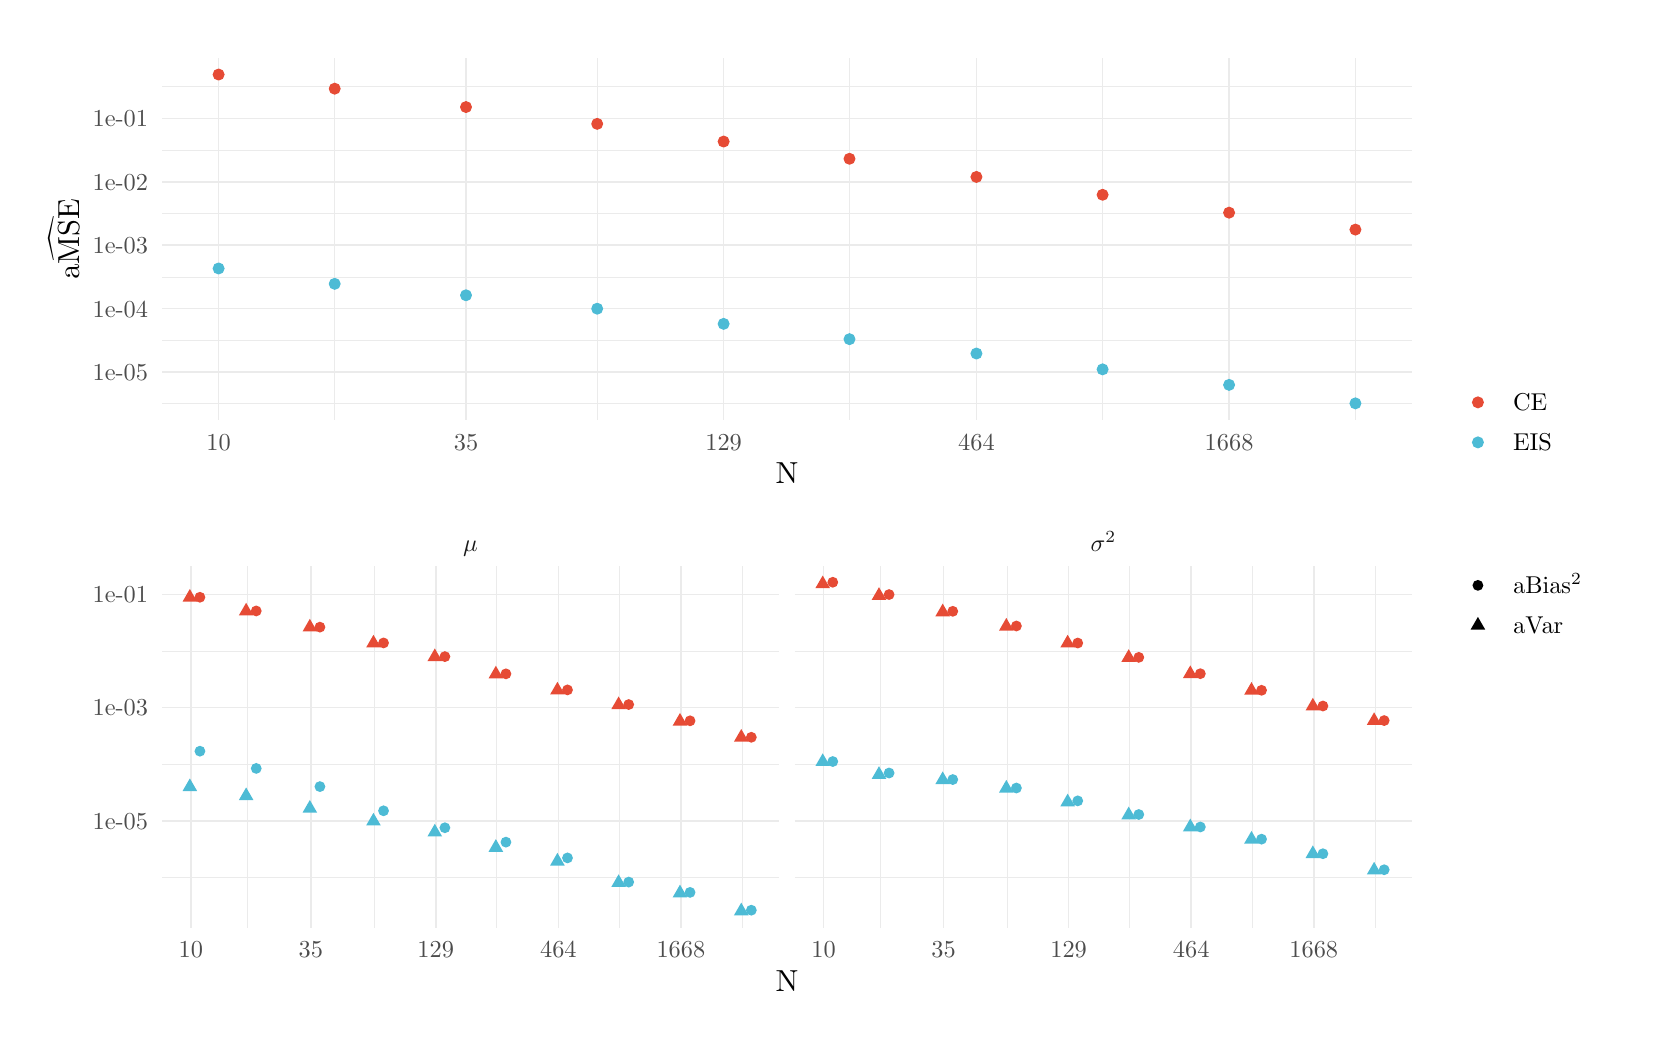
\begin{tikzpicture}[x=1pt,y=1pt]
\definecolor{fillColor}{RGB}{255,255,255}
\path[use as bounding box,fill=fillColor,fill opacity=0.00] (0,0) rectangle (578.16,361.35);
\begin{scope}
\path[clip] ( 48.45,219.65) rectangle (500.31,350.35);
\definecolor{drawColor}{gray}{0.92}

\path[draw=drawColor,line width= 0.3pt,line join=round] ( 48.45,225.46) --
	(500.31,225.46);

\path[draw=drawColor,line width= 0.3pt,line join=round] ( 48.45,248.36) --
	(500.31,248.36);

\path[draw=drawColor,line width= 0.3pt,line join=round] ( 48.45,271.25) --
	(500.31,271.25);

\path[draw=drawColor,line width= 0.3pt,line join=round] ( 48.45,294.15) --
	(500.31,294.15);

\path[draw=drawColor,line width= 0.3pt,line join=round] ( 48.45,317.04) --
	(500.31,317.04);

\path[draw=drawColor,line width= 0.3pt,line join=round] ( 48.45,339.94) --
	(500.31,339.94);

\path[draw=drawColor,line width= 0.3pt,line join=round] (110.94,219.65) --
	(110.94,350.35);

\path[draw=drawColor,line width= 0.3pt,line join=round] (205.79,219.65) --
	(205.79,350.35);

\path[draw=drawColor,line width= 0.3pt,line join=round] (296.96,219.65) --
	(296.96,350.35);

\path[draw=drawColor,line width= 0.3pt,line join=round] (388.42,219.65) --
	(388.42,350.35);

\path[draw=drawColor,line width= 0.3pt,line join=round] (479.78,219.65) --
	(479.78,350.35);

\path[draw=drawColor,line width= 0.6pt,line join=round] ( 48.45,236.91) --
	(500.31,236.91);

\path[draw=drawColor,line width= 0.6pt,line join=round] ( 48.45,259.81) --
	(500.31,259.81);

\path[draw=drawColor,line width= 0.6pt,line join=round] ( 48.45,282.70) --
	(500.31,282.70);

\path[draw=drawColor,line width= 0.6pt,line join=round] ( 48.45,305.60) --
	(500.31,305.60);

\path[draw=drawColor,line width= 0.6pt,line join=round] ( 48.45,328.49) --
	(500.31,328.49);

\path[draw=drawColor,line width= 0.6pt,line join=round] ( 68.99,219.65) --
	( 68.99,350.35);

\path[draw=drawColor,line width= 0.6pt,line join=round] (158.39,219.65) --
	(158.39,350.35);

\path[draw=drawColor,line width= 0.6pt,line join=round] (251.48,219.65) --
	(251.48,350.35);

\path[draw=drawColor,line width= 0.6pt,line join=round] (342.83,219.65) --
	(342.83,350.35);

\path[draw=drawColor,line width= 0.6pt,line join=round] (434.13,219.65) --
	(434.13,350.35);
\definecolor{drawColor}{RGB}{230,75,53}
\definecolor{fillColor}{RGB}{230,75,53}

\path[draw=drawColor,line width= 0.4pt,line join=round,line cap=round,fill=fillColor] ( 68.99,344.41) circle (  1.96);

\path[draw=drawColor,line width= 0.4pt,line join=round,line cap=round,fill=fillColor] (110.94,339.30) circle (  1.96);

\path[draw=drawColor,line width= 0.4pt,line join=round,line cap=round,fill=fillColor] (158.39,332.66) circle (  1.96);

\path[draw=drawColor,line width= 0.4pt,line join=round,line cap=round,fill=fillColor] (205.79,326.59) circle (  1.96);

\path[draw=drawColor,line width= 0.4pt,line join=round,line cap=round,fill=fillColor] (251.48,320.20) circle (  1.96);

\path[draw=drawColor,line width= 0.4pt,line join=round,line cap=round,fill=fillColor] (296.96,313.97) circle (  1.96);

\path[draw=drawColor,line width= 0.4pt,line join=round,line cap=round,fill=fillColor] (342.83,307.41) circle (  1.96);

\path[draw=drawColor,line width= 0.4pt,line join=round,line cap=round,fill=fillColor] (388.42,300.96) circle (  1.96);

\path[draw=drawColor,line width= 0.4pt,line join=round,line cap=round,fill=fillColor] (434.13,294.50) circle (  1.96);

\path[draw=drawColor,line width= 0.4pt,line join=round,line cap=round,fill=fillColor] (479.78,288.38) circle (  1.96);
\definecolor{drawColor}{RGB}{77,187,213}
\definecolor{fillColor}{RGB}{77,187,213}

\path[draw=drawColor,line width= 0.4pt,line join=round,line cap=round,fill=fillColor] ( 68.99,274.33) circle (  1.96);

\path[draw=drawColor,line width= 0.4pt,line join=round,line cap=round,fill=fillColor] (110.94,268.78) circle (  1.96);

\path[draw=drawColor,line width= 0.4pt,line join=round,line cap=round,fill=fillColor] (158.39,264.65) circle (  1.96);

\path[draw=drawColor,line width= 0.4pt,line join=round,line cap=round,fill=fillColor] (205.79,259.80) circle (  1.96);

\path[draw=drawColor,line width= 0.4pt,line join=round,line cap=round,fill=fillColor] (251.48,254.32) circle (  1.96);

\path[draw=drawColor,line width= 0.4pt,line join=round,line cap=round,fill=fillColor] (296.96,248.79) circle (  1.96);

\path[draw=drawColor,line width= 0.4pt,line join=round,line cap=round,fill=fillColor] (342.83,243.60) circle (  1.96);

\path[draw=drawColor,line width= 0.4pt,line join=round,line cap=round,fill=fillColor] (388.42,237.88) circle (  1.96);

\path[draw=drawColor,line width= 0.4pt,line join=round,line cap=round,fill=fillColor] (434.13,232.27) circle (  1.96);

\path[draw=drawColor,line width= 0.4pt,line join=round,line cap=round,fill=fillColor] (479.78,225.59) circle (  1.96);
\end{scope}
\begin{scope}
\path[clip] (  0.00,  0.00) rectangle (578.16,361.35);
\definecolor{drawColor}{gray}{0.30}

\node[text=drawColor,anchor=base east,inner sep=0pt, outer sep=0pt, scale=  0.88] at ( 43.50,233.88) {1e-05};

\node[text=drawColor,anchor=base east,inner sep=0pt, outer sep=0pt, scale=  0.88] at ( 43.50,256.78) {1e-04};

\node[text=drawColor,anchor=base east,inner sep=0pt, outer sep=0pt, scale=  0.88] at ( 43.50,279.67) {1e-03};

\node[text=drawColor,anchor=base east,inner sep=0pt, outer sep=0pt, scale=  0.88] at ( 43.50,302.57) {1e-02};

\node[text=drawColor,anchor=base east,inner sep=0pt, outer sep=0pt, scale=  0.88] at ( 43.50,325.46) {1e-01};
\end{scope}
\begin{scope}
\path[clip] (  0.00,  0.00) rectangle (578.16,361.35);
\definecolor{drawColor}{gray}{0.30}

\node[text=drawColor,anchor=base,inner sep=0pt, outer sep=0pt, scale=  0.88] at ( 68.99,208.64) {10};

\node[text=drawColor,anchor=base,inner sep=0pt, outer sep=0pt, scale=  0.88] at (158.39,208.64) {35};

\node[text=drawColor,anchor=base,inner sep=0pt, outer sep=0pt, scale=  0.88] at (251.48,208.64) {129};

\node[text=drawColor,anchor=base,inner sep=0pt, outer sep=0pt, scale=  0.88] at (342.83,208.64) {464};

\node[text=drawColor,anchor=base,inner sep=0pt, outer sep=0pt, scale=  0.88] at (434.13,208.64) {1668};
\end{scope}
\begin{scope}
\path[clip] (  0.00,  0.00) rectangle (578.16,361.35);
\definecolor{drawColor}{RGB}{0,0,0}

\node[text=drawColor,anchor=base,inner sep=0pt, outer sep=0pt, scale=  1.10] at (274.38,196.60) {N};
\end{scope}
\begin{scope}
\path[clip] (  0.00,  0.00) rectangle (578.16,361.35);
\definecolor{drawColor}{RGB}{0,0,0}

\node[text=drawColor,rotate= 90.00,anchor=base,inner sep=0pt, outer sep=0pt, scale=  1.10] at ( 18.58,285.00) {$\widehat{\mathrm{aMSE}}$};
\end{scope}
\begin{scope}
\path[clip] ( 48.45, 36.19) rectangle (271.63,166.89);
\definecolor{drawColor}{gray}{0.92}

\path[draw=drawColor,line width= 0.3pt,line join=round] ( 48.45, 54.35) --
	(271.63, 54.35);

\path[draw=drawColor,line width= 0.3pt,line join=round] ( 48.45, 95.22) --
	(271.63, 95.22);

\path[draw=drawColor,line width= 0.3pt,line join=round] ( 48.45,136.10) --
	(271.63,136.10);

\path[draw=drawColor,line width= 0.3pt,line join=round] ( 79.29, 36.19) --
	( 79.29,166.89);

\path[draw=drawColor,line width= 0.3pt,line join=round] (125.29, 36.19) --
	(125.29,166.89);

\path[draw=drawColor,line width= 0.3pt,line join=round] (169.52, 36.19) --
	(169.52,166.89);

\path[draw=drawColor,line width= 0.3pt,line join=round] (213.88, 36.19) --
	(213.88,166.89);

\path[draw=drawColor,line width= 0.3pt,line join=round] (258.19, 36.19) --
	(258.19,166.89);

\path[draw=drawColor,line width= 0.6pt,line join=round] ( 48.45, 74.78) --
	(271.63, 74.78);

\path[draw=drawColor,line width= 0.6pt,line join=round] ( 48.45,115.66) --
	(271.63,115.66);

\path[draw=drawColor,line width= 0.6pt,line join=round] ( 48.45,156.54) --
	(271.63,156.54);

\path[draw=drawColor,line width= 0.6pt,line join=round] ( 58.94, 36.19) --
	( 58.94,166.89);

\path[draw=drawColor,line width= 0.6pt,line join=round] (102.31, 36.19) --
	(102.31,166.89);

\path[draw=drawColor,line width= 0.6pt,line join=round] (147.46, 36.19) --
	(147.46,166.89);

\path[draw=drawColor,line width= 0.6pt,line join=round] (191.76, 36.19) --
	(191.76,166.89);

\path[draw=drawColor,line width= 0.6pt,line join=round] (236.05, 36.19) --
	(236.05,166.89);
\definecolor{fillColor}{RGB}{230,75,53}

\path[fill=fillColor] ( 62.24,155.53) circle (  1.96);

\path[fill=fillColor] ( 58.60,158.52) --
	( 61.24,153.94) --
	( 55.96,153.94) --
	cycle;
\definecolor{fillColor}{RGB}{77,187,213}

\path[fill=fillColor] ( 62.24, 99.91) circle (  1.96);

\path[fill=fillColor] ( 58.60, 90.07) --
	( 61.24, 85.50) --
	( 55.96, 85.50) --
	cycle;
\definecolor{fillColor}{RGB}{230,75,53}

\path[fill=fillColor] ( 82.59,150.58) circle (  1.96);

\path[fill=fillColor] ( 78.94,153.54) --
	( 81.59,148.96) --
	( 76.30,148.96) --
	cycle;
\definecolor{fillColor}{RGB}{77,187,213}

\path[fill=fillColor] ( 82.59, 93.68) circle (  1.96);

\path[fill=fillColor] ( 78.94, 86.81) --
	( 81.59, 82.23) --
	( 76.30, 82.23) --
	cycle;
\definecolor{fillColor}{RGB}{230,75,53}

\path[fill=fillColor] (105.60,144.73) circle (  1.96);

\path[fill=fillColor] (101.96,147.73) --
	(104.60,143.16) --
	( 99.32,143.16) --
	cycle;
\definecolor{fillColor}{RGB}{77,187,213}

\path[fill=fillColor] (105.60, 87.11) circle (  1.96);

\path[fill=fillColor] (101.96, 82.27) --
	(104.60, 77.69) --
	( 99.32, 77.69) --
	cycle;
\definecolor{fillColor}{RGB}{230,75,53}

\path[fill=fillColor] (128.59,139.02) circle (  1.96);

\path[fill=fillColor] (124.95,141.97) --
	(127.59,137.39) --
	(122.31,137.39) --
	cycle;
\definecolor{fillColor}{RGB}{77,187,213}

\path[fill=fillColor] (128.59, 78.37) circle (  1.96);

\path[fill=fillColor] (124.95, 77.65) --
	(127.59, 73.08) --
	(122.31, 73.08) --
	cycle;
\definecolor{fillColor}{RGB}{230,75,53}

\path[fill=fillColor] (150.76,134.08) circle (  1.96);

\path[fill=fillColor] (147.11,137.03) --
	(149.76,132.45) --
	(144.47,132.45) --
	cycle;
\definecolor{fillColor}{RGB}{77,187,213}

\path[fill=fillColor] (150.76, 72.24) circle (  1.96);

\path[fill=fillColor] (147.11, 73.68) --
	(149.76, 69.11) --
	(144.47, 69.11) --
	cycle;
\definecolor{fillColor}{RGB}{230,75,53}

\path[fill=fillColor] (172.82,127.85) circle (  1.96);

\path[fill=fillColor] (169.17,130.78) --
	(171.82,126.20) --
	(166.53,126.20) --
	cycle;
\definecolor{fillColor}{RGB}{77,187,213}

\path[fill=fillColor] (172.82, 67.04) circle (  1.96);

\path[fill=fillColor] (169.17, 68.14) --
	(171.82, 63.56) --
	(166.53, 63.56) --
	cycle;
\definecolor{fillColor}{RGB}{230,75,53}

\path[fill=fillColor] (195.06,122.05) circle (  1.96);

\path[fill=fillColor] (191.42,124.98) --
	(194.06,120.40) --
	(188.78,120.40) --
	cycle;
\definecolor{fillColor}{RGB}{77,187,213}

\path[fill=fillColor] (195.06, 61.34) circle (  1.96);

\path[fill=fillColor] (191.42, 63.18) --
	(194.06, 58.60) --
	(188.78, 58.60) --
	cycle;
\definecolor{fillColor}{RGB}{230,75,53}

\path[fill=fillColor] (217.18,116.76) circle (  1.96);

\path[fill=fillColor] (213.53,119.68) --
	(216.18,115.11) --
	(210.89,115.11) --
	cycle;
\definecolor{fillColor}{RGB}{77,187,213}

\path[fill=fillColor] (217.18, 52.61) circle (  1.96);

\path[fill=fillColor] (213.53, 55.43) --
	(216.18, 50.85) --
	(210.89, 50.85) --
	cycle;
\definecolor{fillColor}{RGB}{230,75,53}

\path[fill=fillColor] (239.35,110.88) circle (  1.96);

\path[fill=fillColor] (235.71,113.73) --
	(238.35,109.15) --
	(233.07,109.15) --
	cycle;
\definecolor{fillColor}{RGB}{77,187,213}

\path[fill=fillColor] (239.35, 48.88) circle (  1.96);

\path[fill=fillColor] (235.71, 51.68) --
	(238.35, 47.10) --
	(233.07, 47.10) --
	cycle;
\definecolor{fillColor}{RGB}{230,75,53}

\path[fill=fillColor] (261.49,104.93) circle (  1.96);

\path[fill=fillColor] (257.85,107.91) --
	(260.49,103.33) --
	(255.20,103.33) --
	cycle;
\definecolor{fillColor}{RGB}{77,187,213}

\path[fill=fillColor] (261.49, 42.45) circle (  1.96);

\path[fill=fillColor] (257.85, 45.18) --
	(260.49, 40.60) --
	(255.20, 40.60) --
	cycle;
\end{scope}
\begin{scope}
\path[clip] (277.13, 36.19) rectangle (500.31,166.89);
\definecolor{drawColor}{gray}{0.92}

\path[draw=drawColor,line width= 0.3pt,line join=round] (277.13, 54.35) --
	(500.31, 54.35);

\path[draw=drawColor,line width= 0.3pt,line join=round] (277.13, 95.22) --
	(500.31, 95.22);

\path[draw=drawColor,line width= 0.3pt,line join=round] (277.13,136.10) --
	(500.31,136.10);

\path[draw=drawColor,line width= 0.3pt,line join=round] (307.97, 36.19) --
	(307.97,166.89);

\path[draw=drawColor,line width= 0.3pt,line join=round] (353.97, 36.19) --
	(353.97,166.89);

\path[draw=drawColor,line width= 0.3pt,line join=round] (398.20, 36.19) --
	(398.20,166.89);

\path[draw=drawColor,line width= 0.3pt,line join=round] (442.56, 36.19) --
	(442.56,166.89);

\path[draw=drawColor,line width= 0.3pt,line join=round] (486.87, 36.19) --
	(486.87,166.89);

\path[draw=drawColor,line width= 0.6pt,line join=round] (277.13, 74.78) --
	(500.31, 74.78);

\path[draw=drawColor,line width= 0.6pt,line join=round] (277.13,115.66) --
	(500.31,115.66);

\path[draw=drawColor,line width= 0.6pt,line join=round] (277.13,156.54) --
	(500.31,156.54);

\path[draw=drawColor,line width= 0.6pt,line join=round] (287.62, 36.19) --
	(287.62,166.89);

\path[draw=drawColor,line width= 0.6pt,line join=round] (330.99, 36.19) --
	(330.99,166.89);

\path[draw=drawColor,line width= 0.6pt,line join=round] (376.14, 36.19) --
	(376.14,166.89);

\path[draw=drawColor,line width= 0.6pt,line join=round] (420.45, 36.19) --
	(420.45,166.89);

\path[draw=drawColor,line width= 0.6pt,line join=round] (464.73, 36.19) --
	(464.73,166.89);
\definecolor{fillColor}{RGB}{230,75,53}

\path[fill=fillColor] (290.92,160.95) circle (  1.96);

\path[fill=fillColor] (287.28,163.39) --
	(289.92,158.82) --
	(284.64,158.82) --
	cycle;
\definecolor{fillColor}{RGB}{77,187,213}

\path[fill=fillColor] (290.92, 96.17) circle (  1.96);

\path[fill=fillColor] (287.28, 99.14) --
	(289.92, 94.56) --
	(284.64, 94.56) --
	cycle;
\definecolor{fillColor}{RGB}{230,75,53}

\path[fill=fillColor] (311.27,156.50) circle (  1.96);

\path[fill=fillColor] (307.62,159.16) --
	(310.27,154.59) --
	(304.98,154.59) --
	cycle;
\definecolor{fillColor}{RGB}{77,187,213}

\path[fill=fillColor] (311.27, 92.02) circle (  1.96);

\path[fill=fillColor] (307.62, 94.48) --
	(310.27, 89.90) --
	(304.98, 89.90) --
	cycle;
\definecolor{fillColor}{RGB}{230,75,53}

\path[fill=fillColor] (334.28,150.45) circle (  1.96);

\path[fill=fillColor] (330.64,153.24) --
	(333.28,148.66) --
	(328.00,148.66) --
	cycle;
\definecolor{fillColor}{RGB}{77,187,213}

\path[fill=fillColor] (334.28, 89.66) circle (  1.96);

\path[fill=fillColor] (330.64, 92.60) --
	(333.28, 88.03) --
	(328.00, 88.03) --
	cycle;
\definecolor{fillColor}{RGB}{230,75,53}

\path[fill=fillColor] (357.27,145.14) circle (  1.96);

\path[fill=fillColor] (353.63,148.06) --
	(356.27,143.48) --
	(350.99,143.48) --
	cycle;
\definecolor{fillColor}{RGB}{77,187,213}

\path[fill=fillColor] (357.27, 86.60) circle (  1.96);

\path[fill=fillColor] (353.63, 89.53) --
	(356.27, 84.96) --
	(350.99, 84.96) --
	cycle;
\definecolor{fillColor}{RGB}{230,75,53}

\path[fill=fillColor] (379.44,138.99) circle (  1.96);

\path[fill=fillColor] (375.79,141.98) --
	(378.44,137.40) --
	(373.15,137.40) --
	cycle;
\definecolor{fillColor}{RGB}{77,187,213}

\path[fill=fillColor] (379.44, 81.96) circle (  1.96);

\path[fill=fillColor] (375.79, 84.57) --
	(378.44, 79.99) --
	(373.15, 79.99) --
	cycle;
\definecolor{fillColor}{RGB}{230,75,53}

\path[fill=fillColor] (401.50,133.81) circle (  1.96);

\path[fill=fillColor] (397.85,136.77) --
	(400.50,132.19) --
	(395.21,132.19) --
	cycle;
\definecolor{fillColor}{RGB}{77,187,213}

\path[fill=fillColor] (401.50, 77.03) circle (  1.96);

\path[fill=fillColor] (397.85, 79.89) --
	(400.50, 75.31) --
	(395.21, 75.31) --
	cycle;
\definecolor{fillColor}{RGB}{230,75,53}

\path[fill=fillColor] (423.74,127.91) circle (  1.96);

\path[fill=fillColor] (420.10,130.90) --
	(422.74,126.32) --
	(417.46,126.32) --
	cycle;
\definecolor{fillColor}{RGB}{77,187,213}

\path[fill=fillColor] (423.74, 72.52) circle (  1.96);

\path[fill=fillColor] (420.10, 75.55) --
	(422.74, 70.97) --
	(417.46, 70.97) --
	cycle;
\definecolor{fillColor}{RGB}{230,75,53}

\path[fill=fillColor] (445.86,121.91) circle (  1.96);

\path[fill=fillColor] (442.22,124.89) --
	(444.86,120.31) --
	(439.57,120.31) --
	cycle;
\definecolor{fillColor}{RGB}{77,187,213}

\path[fill=fillColor] (445.86, 68.12) circle (  1.96);

\path[fill=fillColor] (442.22, 71.10) --
	(444.86, 66.52) --
	(439.57, 66.52) --
	cycle;
\definecolor{fillColor}{RGB}{230,75,53}

\path[fill=fillColor] (468.03,116.23) circle (  1.96);

\path[fill=fillColor] (464.39,119.19) --
	(467.03,114.61) --
	(461.75,114.61) --
	cycle;
\definecolor{fillColor}{RGB}{77,187,213}

\path[fill=fillColor] (468.03, 62.85) circle (  1.96);

\path[fill=fillColor] (464.39, 65.87) --
	(467.03, 61.29) --
	(461.75, 61.29) --
	cycle;
\definecolor{fillColor}{RGB}{230,75,53}

\path[fill=fillColor] (490.17,110.97) circle (  1.96);

\path[fill=fillColor] (486.53,113.96) --
	(489.17,109.39) --
	(483.88,109.39) --
	cycle;
\definecolor{fillColor}{RGB}{77,187,213}

\path[fill=fillColor] (490.17, 57.06) circle (  1.96);

\path[fill=fillColor] (486.53, 59.93) --
	(489.17, 55.35) --
	(483.88, 55.35) --
	cycle;
\end{scope}
\begin{scope}
\path[clip] ( 48.45,166.89) rectangle (271.63,183.46);
\definecolor{drawColor}{gray}{0.10}

\node[text=drawColor,anchor=base,inner sep=0pt, outer sep=0pt, scale=  0.88] at (160.04,172.14) {$\mu$};
\end{scope}
\begin{scope}
\path[clip] (277.13,166.89) rectangle (500.31,183.46);
\definecolor{drawColor}{gray}{0.10}

\node[text=drawColor,anchor=base,inner sep=0pt, outer sep=0pt, scale=  0.88] at (388.72,172.14) {$\sigma^2$};
\end{scope}
\begin{scope}
\path[clip] (  0.00,  0.00) rectangle (578.16,361.35);
\definecolor{drawColor}{gray}{0.30}

\node[text=drawColor,anchor=base,inner sep=0pt, outer sep=0pt, scale=  0.88] at ( 58.94, 25.18) {10};

\node[text=drawColor,anchor=base,inner sep=0pt, outer sep=0pt, scale=  0.88] at (102.31, 25.18) {35};

\node[text=drawColor,anchor=base,inner sep=0pt, outer sep=0pt, scale=  0.88] at (147.46, 25.18) {129};

\node[text=drawColor,anchor=base,inner sep=0pt, outer sep=0pt, scale=  0.88] at (191.76, 25.18) {464};

\node[text=drawColor,anchor=base,inner sep=0pt, outer sep=0pt, scale=  0.88] at (236.05, 25.18) {1668};
\end{scope}
\begin{scope}
\path[clip] (  0.00,  0.00) rectangle (578.16,361.35);
\definecolor{drawColor}{gray}{0.30}

\node[text=drawColor,anchor=base,inner sep=0pt, outer sep=0pt, scale=  0.88] at (287.62, 25.18) {10};

\node[text=drawColor,anchor=base,inner sep=0pt, outer sep=0pt, scale=  0.88] at (330.99, 25.18) {35};

\node[text=drawColor,anchor=base,inner sep=0pt, outer sep=0pt, scale=  0.88] at (376.14, 25.18) {129};

\node[text=drawColor,anchor=base,inner sep=0pt, outer sep=0pt, scale=  0.88] at (420.45, 25.18) {464};

\node[text=drawColor,anchor=base,inner sep=0pt, outer sep=0pt, scale=  0.88] at (464.73, 25.18) {1668};
\end{scope}
\begin{scope}
\path[clip] (  0.00,  0.00) rectangle (578.16,361.35);
\definecolor{drawColor}{gray}{0.30}

\node[text=drawColor,anchor=base east,inner sep=0pt, outer sep=0pt, scale=  0.88] at ( 43.50, 71.75) {1e-05};

\node[text=drawColor,anchor=base east,inner sep=0pt, outer sep=0pt, scale=  0.88] at ( 43.50,112.63) {1e-03};

\node[text=drawColor,anchor=base east,inner sep=0pt, outer sep=0pt, scale=  0.88] at ( 43.50,153.51) {1e-01};
\end{scope}
\begin{scope}
\path[clip] (  0.00,  0.00) rectangle (578.16,361.35);
\definecolor{drawColor}{RGB}{0,0,0}

\node[text=drawColor,anchor=base,inner sep=0pt, outer sep=0pt, scale=  1.10] at (274.38, 13.14) {N};
\end{scope}
\begin{scope}
\path[clip] (  0.00,  0.00) rectangle (578.16,361.35);
\definecolor{drawColor}{RGB}{230,75,53}
\definecolor{fillColor}{RGB}{230,75,53}

\path[draw=drawColor,line width= 0.4pt,line join=round,line cap=round,fill=fillColor] (524.04,225.95) circle (  1.96);
\end{scope}
\begin{scope}
\path[clip] (  0.00,  0.00) rectangle (578.16,361.35);
\definecolor{drawColor}{RGB}{77,187,213}
\definecolor{fillColor}{RGB}{77,187,213}

\path[draw=drawColor,line width= 0.4pt,line join=round,line cap=round,fill=fillColor] (524.04,211.49) circle (  1.96);
\end{scope}
\begin{scope}
\path[clip] (  0.00,  0.00) rectangle (578.16,361.35);
\definecolor{drawColor}{RGB}{0,0,0}

\node[text=drawColor,anchor=base west,inner sep=0pt, outer sep=0pt, scale=  0.88] at (536.77,222.92) {CE};
\end{scope}
\begin{scope}
\path[clip] (  0.00,  0.00) rectangle (578.16,361.35);
\definecolor{drawColor}{RGB}{0,0,0}

\node[text=drawColor,anchor=base west,inner sep=0pt, outer sep=0pt, scale=  0.88] at (536.77,208.46) {EIS};
\end{scope}
\begin{scope}
\path[clip] (  0.00,  0.00) rectangle (578.16,361.35);
\definecolor{fillColor}{RGB}{0,0,0}

\path[fill=fillColor] (524.04,159.83) circle (  1.96);
\end{scope}
\begin{scope}
\path[clip] (  0.00,  0.00) rectangle (578.16,361.35);
\definecolor{fillColor}{RGB}{0,0,0}

\path[fill=fillColor] (524.04,148.42) --
	(526.68,143.85) --
	(521.40,143.85) --
	cycle;
\end{scope}
\begin{scope}
\path[clip] (  0.00,  0.00) rectangle (578.16,361.35);
\definecolor{drawColor}{RGB}{0,0,0}

\node[text=drawColor,anchor=base west,inner sep=0pt, outer sep=0pt, scale=  0.88] at (536.77,156.80) {aBias$^2$};
\end{scope}
\begin{scope}
\path[clip] (  0.00,  0.00) rectangle (578.16,361.35);
\definecolor{drawColor}{RGB}{0,0,0}

\node[text=drawColor,anchor=base west,inner sep=0pt, outer sep=0pt, scale=  0.88] at (536.77,142.34) {aVar};
\end{scope}
\end{tikzpicture}

    }
    \caption{{\color{red} TODO}}
    \label{fig:mse_bias_var_decomposition}
\end{figure}

% fig:mse_bias_var_decomposition
\todo{interpretation of \Cref{fig:mse_bias_var_decomposition}, equal contribution of bias and var, not much to gain from bias correction}


\subsection{Numerical convergence}
\label{subsec:numerical-convergence}

\subsection{Performance of the optimal proposal}
\label{subsec:performance_at_optimal}
\todo{change EF to aEF (asymptotic EF) everywhere in this section}
For the performance of importance sampling the efficiency factor $ \text{EF} = \frac{\text{ESS}}{N}$ plays an important role, see \Cref{sec:importance_sampling}. Additionally, it allows a comparison of the effectiveness of importance sampling across multiple sample sizes $N$, indeed, as $N\to\infty$, $\text{EF}$ converges to $ \rho^{-1}$, where $\rho$ is the second moment of importance sampling weights, $\int w^{2} \d \G$.

Returning to the distributions studied in \Cref{ex:univ-gaussian-s2-fixed,ex:univ-gaussian-mu-fixed}, we now calculate the asymptotic efficiency factor
$$
\text{EF} = \frac{1}{\rho} \in (0, 1].
$$
As the proposal is always $\mathcal N(\mu, \sigma^{2})$ with either $\mu$ or $\sigma^{2}$ fixed, and $\P$ is a mixture of Gaussians or $\mathcal N(0,1)$, $\rho$ is analytically available. 

For \Cref{ex:univ-gaussian-s2-fixed}, both \aeis and the \acem have, by symmetry, the same optimal $\mu = 0$. Thus the efficiency factor only depends on the fixed $\sigma^{2}$, see \Cref{fig:rho_mu}, and is the same for \aeis and the \acem.

\begin{figure}
    \centering
    \resizebox{\textwidth}{!}{%
        % Created by tikzDevice version 0.12.6 on 2024-06-10 16:57:56
% !TEX encoding = UTF-8 Unicode
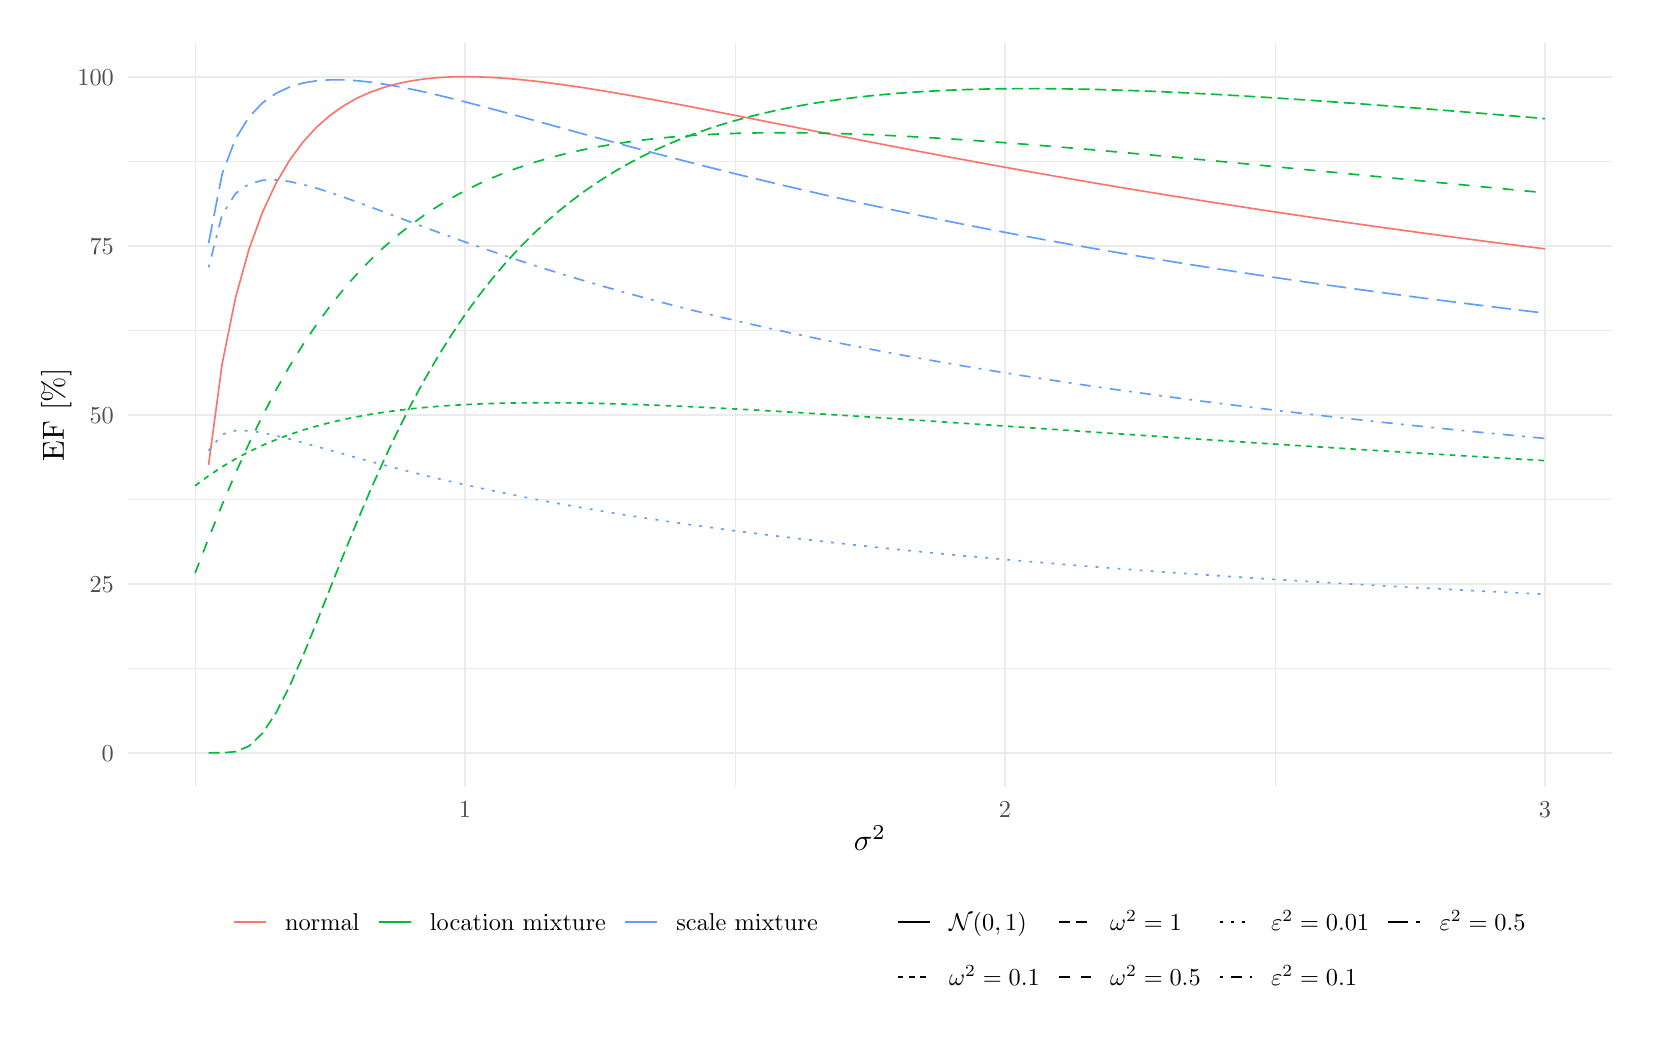
\begin{tikzpicture}[x=1pt,y=1pt]
\definecolor{fillColor}{RGB}{255,255,255}
\path[use as bounding box,fill=fillColor,fill opacity=0.00] (0,0) rectangle (578.16,361.35);
\begin{scope}
\path[clip] ( 36.11, 87.09) rectangle (572.66,355.85);
\definecolor{drawColor}{gray}{0.92}

\path[draw=drawColor,line width= 0.3pt,line join=round] ( 36.11,129.85) --
	(572.66,129.85);

\path[draw=drawColor,line width= 0.3pt,line join=round] ( 36.11,190.93) --
	(572.66,190.93);

\path[draw=drawColor,line width= 0.3pt,line join=round] ( 36.11,252.01) --
	(572.66,252.01);

\path[draw=drawColor,line width= 0.3pt,line join=round] ( 36.11,313.09) --
	(572.66,313.09);

\path[draw=drawColor,line width= 0.3pt,line join=round] ( 60.50, 87.09) --
	( 60.50,355.85);

\path[draw=drawColor,line width= 0.3pt,line join=round] (255.61, 87.09) --
	(255.61,355.85);

\path[draw=drawColor,line width= 0.3pt,line join=round] (450.72, 87.09) --
	(450.72,355.85);

\path[draw=drawColor,line width= 0.6pt,line join=round] ( 36.11, 99.31) --
	(572.66, 99.31);

\path[draw=drawColor,line width= 0.6pt,line join=round] ( 36.11,160.39) --
	(572.66,160.39);

\path[draw=drawColor,line width= 0.6pt,line join=round] ( 36.11,221.47) --
	(572.66,221.47);

\path[draw=drawColor,line width= 0.6pt,line join=round] ( 36.11,282.55) --
	(572.66,282.55);

\path[draw=drawColor,line width= 0.6pt,line join=round] ( 36.11,343.63) --
	(572.66,343.63);

\path[draw=drawColor,line width= 0.6pt,line join=round] (158.05, 87.09) --
	(158.05,355.85);

\path[draw=drawColor,line width= 0.6pt,line join=round] (353.16, 87.09) --
	(353.16,355.85);

\path[draw=drawColor,line width= 0.6pt,line join=round] (548.27, 87.09) --
	(548.27,355.85);
\definecolor{drawColor}{RGB}{248,118,109}

\path[draw=drawColor,line width= 0.6pt,line join=round] ( 65.38,203.37) --
	( 70.26,239.79) --
	( 75.13,263.88) --
	( 80.01,281.42) --
	( 84.89,294.77) --
	( 89.77,305.19) --
	( 94.64,313.45) --
	( 99.52,320.06) --
	(104.40,325.38) --
	(109.28,329.66) --
	(114.15,333.11) --
	(119.03,335.88) --
	(123.91,338.07) --
	(128.79,339.80) --
	(133.67,341.13) --
	(138.54,342.12) --
	(143.42,342.83) --
	(148.30,343.30) --
	(153.18,343.55) --
	(158.05,343.63) --
	(162.93,343.56) --
	(167.81,343.36) --
	(172.69,343.04) --
	(177.56,342.62) --
	(182.44,342.12) --
	(187.32,341.55) --
	(192.20,340.91) --
	(197.08,340.22) --
	(201.95,339.48) --
	(206.83,338.70) --
	(211.71,337.88) --
	(216.59,337.04) --
	(221.46,336.17) --
	(226.34,335.28) --
	(231.22,334.37) --
	(236.10,333.45) --
	(240.98,332.51) --
	(245.85,331.57) --
	(250.73,330.62) --
	(255.61,329.66) --
	(260.49,328.70) --
	(265.36,327.74) --
	(270.24,326.77) --
	(275.12,325.80) --
	(280.00,324.84) --
	(284.87,323.88) --
	(289.75,322.92) --
	(294.63,321.96) --
	(299.51,321.01) --
	(304.39,320.06) --
	(309.26,319.11) --
	(314.14,318.18) --
	(319.02,317.24) --
	(323.90,316.32) --
	(328.77,315.40) --
	(333.65,314.48) --
	(338.53,313.58) --
	(343.41,312.68) --
	(348.29,311.79) --
	(353.16,310.90) --
	(358.04,310.02) --
	(362.92,309.15) --
	(367.80,308.29) --
	(372.67,307.43) --
	(377.55,306.59) --
	(382.43,305.75) --
	(387.31,304.91) --
	(392.18,304.09) --
	(397.06,303.27) --
	(401.94,302.46) --
	(406.82,301.66) --
	(411.70,300.86) --
	(416.57,300.08) --
	(421.45,299.30) --
	(426.33,298.52) --
	(431.21,297.76) --
	(436.08,297.00) --
	(440.96,296.25) --
	(445.84,295.51) --
	(450.72,294.77) --
	(455.59,294.04) --
	(460.47,293.32) --
	(465.35,292.60) --
	(470.23,291.89) --
	(475.11,291.19) --
	(479.98,290.50) --
	(484.86,289.81) --
	(489.74,289.12) --
	(494.62,288.45) --
	(499.49,287.78) --
	(504.37,287.12) --
	(509.25,286.46) --
	(514.13,285.81) --
	(519.01,285.16) --
	(523.88,284.52) --
	(528.76,283.89) --
	(533.64,283.26) --
	(538.52,282.64) --
	(543.39,282.03) --
	(548.27,281.42);
\definecolor{drawColor}{RGB}{0,186,56}

\path[draw=drawColor,line width= 0.6pt,dash pattern=on 2pt off 2pt ,line join=round] ( 60.50,195.82) --
	( 65.38,199.43) --
	( 70.26,202.66) --
	( 75.13,205.55) --
	( 80.01,208.13) --
	( 84.89,210.43) --
	( 89.77,212.49) --
	( 94.64,214.31) --
	( 99.52,215.93) --
	(104.40,217.37) --
	(109.28,218.65) --
	(114.15,219.77) --
	(119.03,220.76) --
	(123.91,221.63) --
	(128.79,222.39) --
	(133.67,223.05) --
	(138.54,223.62) --
	(143.42,224.10) --
	(148.30,224.52) --
	(153.18,224.86) --
	(158.05,225.14) --
	(162.93,225.37) --
	(167.81,225.54) --
	(172.69,225.67) --
	(177.56,225.75) --
	(182.44,225.80) --
	(187.32,225.81) --
	(192.20,225.79) --
	(197.08,225.74) --
	(201.95,225.66) --
	(206.83,225.56) --
	(211.71,225.43) --
	(216.59,225.29) --
	(221.46,225.12) --
	(226.34,224.94) --
	(231.22,224.74) --
	(236.10,224.53) --
	(240.98,224.31) --
	(245.85,224.07) --
	(250.73,223.83) --
	(255.61,223.57) --
	(260.49,223.31) --
	(265.36,223.03) --
	(270.24,222.75) --
	(275.12,222.46) --
	(280.00,222.17) --
	(284.87,221.87) --
	(289.75,221.57) --
	(294.63,221.26) --
	(299.51,220.95) --
	(304.39,220.63) --
	(309.26,220.32) --
	(314.14,220.00) --
	(319.02,219.67) --
	(323.90,219.35) --
	(328.77,219.02) --
	(333.65,218.70) --
	(338.53,218.37) --
	(343.41,218.04) --
	(348.29,217.71) --
	(353.16,217.38) --
	(358.04,217.05) --
	(362.92,216.71) --
	(367.80,216.38) --
	(372.67,216.05) --
	(377.55,215.72) --
	(382.43,215.39) --
	(387.31,215.06) --
	(392.18,214.73) --
	(397.06,214.41) --
	(401.94,214.08) --
	(406.82,213.75) --
	(411.70,213.43) --
	(416.57,213.10) --
	(421.45,212.78) --
	(426.33,212.46) --
	(431.21,212.14) --
	(436.08,211.82) --
	(440.96,211.50) --
	(445.84,211.18) --
	(450.72,210.87) --
	(455.59,210.56) --
	(460.47,210.24) --
	(465.35,209.93) --
	(470.23,209.63) --
	(475.11,209.32) --
	(479.98,209.01) --
	(484.86,208.71) --
	(489.74,208.41) --
	(494.62,208.11) --
	(499.49,207.81) --
	(504.37,207.51) --
	(509.25,207.21) --
	(514.13,206.92) --
	(519.01,206.63) --
	(523.88,206.34) --
	(528.76,206.05) --
	(533.64,205.76) --
	(538.52,205.48) --
	(543.39,205.19) --
	(548.27,204.91);

\path[draw=drawColor,line width= 0.6pt,dash pattern=on 4pt off 2pt ,line join=round] ( 65.38, 99.31) --
	( 70.26, 99.32) --
	( 75.13, 99.73) --
	( 80.01,101.76) --
	( 84.89,106.42) --
	( 89.77,113.81) --
	( 94.64,123.40) --
	( 99.52,134.49) --
	(104.40,146.43) --
	(109.28,158.70) --
	(114.15,170.93) --
	(119.03,182.87) --
	(123.91,194.33) --
	(128.79,205.24) --
	(133.67,215.53) --
	(138.54,225.18) --
	(143.42,234.19) --
	(148.30,242.59) --
	(153.18,250.40) --
	(158.05,257.65) --
	(162.93,264.36) --
	(167.81,270.57) --
	(172.69,276.33) --
	(177.56,281.64) --
	(182.44,286.56) --
	(187.32,291.11) --
	(192.20,295.30) --
	(197.08,299.18) --
	(201.95,302.76) --
	(206.83,306.07) --
	(211.71,309.12) --
	(216.59,311.94) --
	(221.46,314.53) --
	(226.34,316.93) --
	(231.22,319.13) --
	(236.10,321.16) --
	(240.98,323.03) --
	(245.85,324.74) --
	(250.73,326.32) --
	(255.61,327.76) --
	(260.49,329.09) --
	(265.36,330.30) --
	(270.24,331.40) --
	(275.12,332.41) --
	(280.00,333.32) --
	(284.87,334.15) --
	(289.75,334.90) --
	(294.63,335.57) --
	(299.51,336.17) --
	(304.39,336.71) --
	(309.26,337.19) --
	(314.14,337.61) --
	(319.02,337.97) --
	(323.90,338.29) --
	(328.77,338.55) --
	(333.65,338.78) --
	(338.53,338.96) --
	(343.41,339.10) --
	(348.29,339.21) --
	(353.16,339.28) --
	(358.04,339.32) --
	(362.92,339.33) --
	(367.80,339.31) --
	(372.67,339.26) --
	(377.55,339.19) --
	(382.43,339.10) --
	(387.31,338.98) --
	(392.18,338.84) --
	(397.06,338.68) --
	(401.94,338.51) --
	(406.82,338.32) --
	(411.70,338.11) --
	(416.57,337.88) --
	(421.45,337.64) --
	(426.33,337.39) --
	(431.21,337.13) --
	(436.08,336.85) --
	(440.96,336.56) --
	(445.84,336.26) --
	(450.72,335.96) --
	(455.59,335.64) --
	(460.47,335.31) --
	(465.35,334.98) --
	(470.23,334.64) --
	(475.11,334.29) --
	(479.98,333.94) --
	(484.86,333.57) --
	(489.74,333.21) --
	(494.62,332.84) --
	(499.49,332.46) --
	(504.37,332.08) --
	(509.25,331.69) --
	(514.13,331.30) --
	(519.01,330.91) --
	(523.88,330.51) --
	(528.76,330.11) --
	(533.64,329.71) --
	(538.52,329.30) --
	(543.39,328.89) --
	(548.27,328.48);

\path[draw=drawColor,line width= 0.6pt,dash pattern=on 4pt off 4pt ,line join=round] ( 60.50,164.25) --
	( 65.38,176.83) --
	( 70.26,188.93) --
	( 75.13,200.39) --
	( 80.01,211.15) --
	( 84.89,221.17) --
	( 89.77,230.45) --
	( 94.64,239.01) --
	( 99.52,246.89) --
	(104.40,254.12) --
	(109.28,260.75) --
	(114.15,266.83) --
	(119.03,272.38) --
	(123.91,277.45) --
	(128.79,282.09) --
	(133.67,286.32) --
	(138.54,290.17) --
	(143.42,293.69) --
	(148.30,296.89) --
	(153.18,299.81) --
	(158.05,302.46) --
	(162.93,304.87) --
	(167.81,307.06) --
	(172.69,309.05) --
	(177.56,310.84) --
	(182.44,312.46) --
	(187.32,313.93) --
	(192.20,315.25) --
	(197.08,316.43) --
	(201.95,317.49) --
	(206.83,318.43) --
	(211.71,319.26) --
	(216.59,320.00) --
	(221.46,320.65) --
	(226.34,321.21) --
	(231.22,321.70) --
	(236.10,322.11) --
	(240.98,322.46) --
	(245.85,322.74) --
	(250.73,322.97) --
	(255.61,323.15) --
	(260.49,323.27) --
	(265.36,323.35) --
	(270.24,323.39) --
	(275.12,323.39) --
	(280.00,323.35) --
	(284.87,323.27) --
	(289.75,323.17) --
	(294.63,323.04) --
	(299.51,322.88) --
	(304.39,322.69) --
	(309.26,322.48) --
	(314.14,322.25) --
	(319.02,322.00) --
	(323.90,321.72) --
	(328.77,321.44) --
	(333.65,321.13) --
	(338.53,320.81) --
	(343.41,320.48) --
	(348.29,320.13) --
	(353.16,319.77) --
	(358.04,319.40) --
	(362.92,319.02) --
	(367.80,318.63) --
	(372.67,318.24) --
	(377.55,317.83) --
	(382.43,317.42) --
	(387.31,317.00) --
	(392.18,316.57) --
	(397.06,316.14) --
	(401.94,315.70) --
	(406.82,315.26) --
	(411.70,314.81) --
	(416.57,314.36) --
	(421.45,313.90) --
	(426.33,313.45) --
	(431.21,312.99) --
	(436.08,312.52) --
	(440.96,312.06) --
	(445.84,311.59) --
	(450.72,311.12) --
	(455.59,310.65) --
	(460.47,310.18) --
	(465.35,309.71) --
	(470.23,309.24) --
	(475.11,308.76) --
	(479.98,308.29) --
	(484.86,307.81) --
	(489.74,307.34) --
	(494.62,306.86) --
	(499.49,306.39) --
	(504.37,305.92) --
	(509.25,305.44) --
	(514.13,304.97) --
	(519.01,304.50) --
	(523.88,304.02) --
	(528.76,303.55) --
	(533.64,303.08) --
	(538.52,302.61) --
	(543.39,302.15) --
	(548.27,301.68);
\definecolor{drawColor}{RGB}{97,156,255}

\path[draw=drawColor,line width= 0.6pt,dash pattern=on 1pt off 3pt ,line join=round] ( 65.38,208.48) --
	( 70.26,214.33) --
	( 75.13,215.76) --
	( 80.01,215.71) --
	( 84.89,214.99) --
	( 89.77,213.93) --
	( 94.64,212.70) --
	( 99.52,211.37) --
	(104.40,210.01) --
	(109.28,208.63) --
	(114.15,207.26) --
	(119.03,205.90) --
	(123.91,204.58) --
	(128.79,203.28) --
	(133.67,202.01) --
	(138.54,200.78) --
	(143.42,199.58) --
	(148.30,198.41) --
	(153.18,197.28) --
	(158.05,196.18) --
	(162.93,195.11) --
	(167.81,194.07) --
	(172.69,193.07) --
	(177.56,192.09) --
	(182.44,191.13) --
	(187.32,190.21) --
	(192.20,189.31) --
	(197.08,188.44) --
	(201.95,187.58) --
	(206.83,186.76) --
	(211.71,185.95) --
	(216.59,185.16) --
	(221.46,184.40) --
	(226.34,183.65) --
	(231.22,182.92) --
	(236.10,182.21) --
	(240.98,181.52) --
	(245.85,180.85) --
	(250.73,180.19) --
	(255.61,179.54) --
	(260.49,178.91) --
	(265.36,178.30) --
	(270.24,177.70) --
	(275.12,177.11) --
	(280.00,176.53) --
	(284.87,175.97) --
	(289.75,175.42) --
	(294.63,174.88) --
	(299.51,174.35) --
	(304.39,173.83) --
	(309.26,173.32) --
	(314.14,172.83) --
	(319.02,172.34) --
	(323.90,171.86) --
	(328.77,171.39) --
	(333.65,170.93) --
	(338.53,170.48) --
	(343.41,170.04) --
	(348.29,169.60) --
	(353.16,169.17) --
	(358.04,168.75) --
	(362.92,168.34) --
	(367.80,167.94) --
	(372.67,167.54) --
	(377.55,167.15) --
	(382.43,166.76) --
	(387.31,166.38) --
	(392.18,166.01) --
	(397.06,165.65) --
	(401.94,165.29) --
	(406.82,164.93) --
	(411.70,164.58) --
	(416.57,164.24) --
	(421.45,163.90) --
	(426.33,163.57) --
	(431.21,163.24) --
	(436.08,162.92) --
	(440.96,162.60) --
	(445.84,162.29) --
	(450.72,161.98) --
	(455.59,161.68) --
	(460.47,161.38) --
	(465.35,161.08) --
	(470.23,160.79) --
	(475.11,160.50) --
	(479.98,160.22) --
	(484.86,159.94) --
	(489.74,159.66) --
	(494.62,159.39) --
	(499.49,159.12) --
	(504.37,158.86) --
	(509.25,158.60) --
	(514.13,158.34) --
	(519.01,158.08) --
	(523.88,157.83) --
	(528.76,157.58) --
	(533.64,157.34) --
	(538.52,157.10) --
	(543.39,156.86) --
	(548.27,156.62);

\path[draw=drawColor,line width= 0.6pt,dash pattern=on 1pt off 3pt on 4pt off 3pt ,line join=round] ( 65.38,274.74) --
	( 70.26,293.74) --
	( 75.13,301.44) --
	( 80.01,304.87) --
	( 84.89,306.20) --
	( 89.77,306.33) --
	( 94.64,305.74) --
	( 99.52,304.68) --
	(104.40,303.33) --
	(109.28,301.78) --
	(114.15,300.11) --
	(119.03,298.35) --
	(123.91,296.55) --
	(128.79,294.72) --
	(133.67,292.88) --
	(138.54,291.05) --
	(143.42,289.23) --
	(148.30,287.43) --
	(153.18,285.66) --
	(158.05,283.91) --
	(162.93,282.19) --
	(167.81,280.51) --
	(172.69,278.86) --
	(177.56,277.24) --
	(182.44,275.65) --
	(187.32,274.10) --
	(192.20,272.58) --
	(197.08,271.09) --
	(201.95,269.63) --
	(206.83,268.21) --
	(211.71,266.82) --
	(216.59,265.45) --
	(221.46,264.12) --
	(226.34,262.81) --
	(231.22,261.54) --
	(236.10,260.28) --
	(240.98,259.06) --
	(245.85,257.86) --
	(250.73,256.68) --
	(255.61,255.53) --
	(260.49,254.41) --
	(265.36,253.30) --
	(270.24,252.22) --
	(275.12,251.16) --
	(280.00,250.12) --
	(284.87,249.09) --
	(289.75,248.09) --
	(294.63,247.11) --
	(299.51,246.15) --
	(304.39,245.20) --
	(309.26,244.27) --
	(314.14,243.36) --
	(319.02,242.46) --
	(323.90,241.58) --
	(328.77,240.72) --
	(333.65,239.87) --
	(338.53,239.04) --
	(343.41,238.22) --
	(348.29,237.41) --
	(353.16,236.62) --
	(358.04,235.84) --
	(362.92,235.07) --
	(367.80,234.32) --
	(372.67,233.58) --
	(377.55,232.85) --
	(382.43,232.13) --
	(387.31,231.42) --
	(392.18,230.72) --
	(397.06,230.04) --
	(401.94,229.36) --
	(406.82,228.70) --
	(411.70,228.04) --
	(416.57,227.40) --
	(421.45,226.76) --
	(426.33,226.13) --
	(431.21,225.51) --
	(436.08,224.91) --
	(440.96,224.31) --
	(445.84,223.71) --
	(450.72,223.13) --
	(455.59,222.55) --
	(460.47,221.99) --
	(465.35,221.43) --
	(470.23,220.87) --
	(475.11,220.33) --
	(479.98,219.79) --
	(484.86,219.26) --
	(489.74,218.73) --
	(494.62,218.22) --
	(499.49,217.71) --
	(504.37,217.20) --
	(509.25,216.70) --
	(514.13,216.21) --
	(519.01,215.72) --
	(523.88,215.24) --
	(528.76,214.77) --
	(533.64,214.30) --
	(538.52,213.84) --
	(543.39,213.38) --
	(548.27,212.93);

\path[draw=drawColor,line width= 0.6pt,dash pattern=on 7pt off 3pt ,line join=round] ( 65.38,283.45) --
	( 70.26,308.45) --
	( 75.13,321.26) --
	( 80.01,329.09) --
	( 84.89,334.21) --
	( 89.77,337.63) --
	( 94.64,339.90) --
	( 99.52,341.33) --
	(104.40,342.15) --
	(109.28,342.50) --
	(114.15,342.48) --
	(119.03,342.18) --
	(123.91,341.66) --
	(128.79,340.95) --
	(133.67,340.11) --
	(138.54,339.14) --
	(143.42,338.09) --
	(148.30,336.96) --
	(153.18,335.77) --
	(158.05,334.54) --
	(162.93,333.27) --
	(167.81,331.97) --
	(172.69,330.66) --
	(177.56,329.33) --
	(182.44,327.99) --
	(187.32,326.65) --
	(192.20,325.30) --
	(197.08,323.96) --
	(201.95,322.62) --
	(206.83,321.29) --
	(211.71,319.97) --
	(216.59,318.65) --
	(221.46,317.35) --
	(226.34,316.05) --
	(231.22,314.77) --
	(236.10,313.51) --
	(240.98,312.25) --
	(245.85,311.01) --
	(250.73,309.79) --
	(255.61,308.58) --
	(260.49,307.38) --
	(265.36,306.20) --
	(270.24,305.03) --
	(275.12,303.88) --
	(280.00,302.74) --
	(284.87,301.62) --
	(289.75,300.51) --
	(294.63,299.42) --
	(299.51,298.34) --
	(304.39,297.28) --
	(309.26,296.23) --
	(314.14,295.19) --
	(319.02,294.17) --
	(323.90,293.16) --
	(328.77,292.16) --
	(333.65,291.18) --
	(338.53,290.21) --
	(343.41,289.26) --
	(348.29,288.31) --
	(353.16,287.38) --
	(358.04,286.46) --
	(362.92,285.56) --
	(367.80,284.66) --
	(372.67,283.78) --
	(377.55,282.91) --
	(382.43,282.04) --
	(387.31,281.19) --
	(392.18,280.36) --
	(397.06,279.53) --
	(401.94,278.71) --
	(406.82,277.90) --
	(411.70,277.10) --
	(416.57,276.31) --
	(421.45,275.54) --
	(426.33,274.77) --
	(431.21,274.01) --
	(436.08,273.26) --
	(440.96,272.52) --
	(445.84,271.79) --
	(450.72,271.06) --
	(455.59,270.35) --
	(460.47,269.64) --
	(465.35,268.94) --
	(470.23,268.25) --
	(475.11,267.57) --
	(479.98,266.89) --
	(484.86,266.23) --
	(489.74,265.57) --
	(494.62,264.92) --
	(499.49,264.27) --
	(504.37,263.63) --
	(509.25,263.00) --
	(514.13,262.38) --
	(519.01,261.76) --
	(523.88,261.15) --
	(528.76,260.55) --
	(533.64,259.95) --
	(538.52,259.36) --
	(543.39,258.78) --
	(548.27,258.20);
\end{scope}
\begin{scope}
\path[clip] (  0.00,  0.00) rectangle (578.16,361.35);
\definecolor{drawColor}{gray}{0.30}

\node[text=drawColor,anchor=base east,inner sep=0pt, outer sep=0pt, scale=  0.88] at ( 31.16, 96.28) {0};

\node[text=drawColor,anchor=base east,inner sep=0pt, outer sep=0pt, scale=  0.88] at ( 31.16,157.36) {25};

\node[text=drawColor,anchor=base east,inner sep=0pt, outer sep=0pt, scale=  0.88] at ( 31.16,218.44) {50};

\node[text=drawColor,anchor=base east,inner sep=0pt, outer sep=0pt, scale=  0.88] at ( 31.16,279.52) {75};

\node[text=drawColor,anchor=base east,inner sep=0pt, outer sep=0pt, scale=  0.88] at ( 31.16,340.60) {100};
\end{scope}
\begin{scope}
\path[clip] (  0.00,  0.00) rectangle (578.16,361.35);
\definecolor{drawColor}{gray}{0.30}

\node[text=drawColor,anchor=base,inner sep=0pt, outer sep=0pt, scale=  0.88] at (158.05, 76.08) {1};

\node[text=drawColor,anchor=base,inner sep=0pt, outer sep=0pt, scale=  0.88] at (353.16, 76.08) {2};

\node[text=drawColor,anchor=base,inner sep=0pt, outer sep=0pt, scale=  0.88] at (548.27, 76.08) {3};
\end{scope}
\begin{scope}
\path[clip] (  0.00,  0.00) rectangle (578.16,361.35);
\definecolor{drawColor}{RGB}{0,0,0}

\node[text=drawColor,anchor=base,inner sep=0pt, outer sep=0pt, scale=  1.10] at (304.39, 64.05) {$\sigma^2$};
\end{scope}
\begin{scope}
\path[clip] (  0.00,  0.00) rectangle (578.16,361.35);
\definecolor{drawColor}{RGB}{0,0,0}

\node[text=drawColor,rotate= 90.00,anchor=base,inner sep=0pt, outer sep=0pt, scale=  1.10] at ( 13.08,221.47) {EF [\%]};
\end{scope}
\begin{scope}
\path[clip] (  0.00,  0.00) rectangle (578.16,361.35);
\definecolor{drawColor}{RGB}{248,118,109}

\path[draw=drawColor,line width= 0.6pt,line join=round] ( 74.48, 38.18) -- ( 86.05, 38.18);
\end{scope}
\begin{scope}
\path[clip] (  0.00,  0.00) rectangle (578.16,361.35);
\definecolor{drawColor}{RGB}{0,186,56}

\path[draw=drawColor,line width= 0.6pt,line join=round] (126.84, 38.18) -- (138.41, 38.18);
\end{scope}
\begin{scope}
\path[clip] (  0.00,  0.00) rectangle (578.16,361.35);
\definecolor{drawColor}{RGB}{97,156,255}

\path[draw=drawColor,line width= 0.6pt,line join=round] (215.86, 38.18) -- (227.43, 38.18);
\end{scope}
\begin{scope}
\path[clip] (  0.00,  0.00) rectangle (578.16,361.35);
\definecolor{drawColor}{RGB}{0,0,0}

\node[text=drawColor,anchor=base west,inner sep=0pt, outer sep=0pt, scale=  0.88] at ( 92.99, 35.15) {normal};
\end{scope}
\begin{scope}
\path[clip] (  0.00,  0.00) rectangle (578.16,361.35);
\definecolor{drawColor}{RGB}{0,0,0}

\node[text=drawColor,anchor=base west,inner sep=0pt, outer sep=0pt, scale=  0.88] at (145.35, 35.15) {location mixture};
\end{scope}
\begin{scope}
\path[clip] (  0.00,  0.00) rectangle (578.16,361.35);
\definecolor{drawColor}{RGB}{0,0,0}

\node[text=drawColor,anchor=base west,inner sep=0pt, outer sep=0pt, scale=  0.88] at (234.37, 35.15) {scale mixture};
\end{scope}
\begin{scope}
\path[clip] (  0.00,  0.00) rectangle (578.16,361.35);
\definecolor{drawColor}{RGB}{0,0,0}

\path[draw=drawColor,line width= 0.6pt,line join=round] (314.47, 38.18) -- (326.03, 38.18);
\end{scope}
\begin{scope}
\path[clip] (  0.00,  0.00) rectangle (578.16,361.35);
\definecolor{drawColor}{RGB}{0,0,0}

\path[draw=drawColor,line width= 0.6pt,dash pattern=on 2pt off 2pt ,line join=round] (314.47, 18.23) -- (326.03, 18.23);
\end{scope}
\begin{scope}
\path[clip] (  0.00,  0.00) rectangle (578.16,361.35);
\definecolor{drawColor}{RGB}{0,0,0}

\path[draw=drawColor,line width= 0.6pt,dash pattern=on 4pt off 2pt ,line join=round] (372.64, 38.18) -- (384.20, 38.18);
\end{scope}
\begin{scope}
\path[clip] (  0.00,  0.00) rectangle (578.16,361.35);
\definecolor{drawColor}{RGB}{0,0,0}

\path[draw=drawColor,line width= 0.6pt,dash pattern=on 4pt off 4pt ,line join=round] (372.64, 18.23) -- (384.20, 18.23);
\end{scope}
\begin{scope}
\path[clip] (  0.00,  0.00) rectangle (578.16,361.35);
\definecolor{drawColor}{RGB}{0,0,0}

\path[draw=drawColor,line width= 0.6pt,dash pattern=on 1pt off 3pt ,line join=round] (430.81, 38.18) -- (442.38, 38.18);
\end{scope}
\begin{scope}
\path[clip] (  0.00,  0.00) rectangle (578.16,361.35);
\definecolor{drawColor}{RGB}{0,0,0}

\path[draw=drawColor,line width= 0.6pt,dash pattern=on 1pt off 3pt on 4pt off 3pt ,line join=round] (430.81, 18.23) -- (442.38, 18.23);
\end{scope}
\begin{scope}
\path[clip] (  0.00,  0.00) rectangle (578.16,361.35);
\definecolor{drawColor}{RGB}{0,0,0}

\path[draw=drawColor,line width= 0.6pt,dash pattern=on 7pt off 3pt ,line join=round] (491.70, 38.18) -- (503.26, 38.18);
\end{scope}
\begin{scope}
\path[clip] (  0.00,  0.00) rectangle (578.16,361.35);
\definecolor{drawColor}{RGB}{0,0,0}

\node[text=drawColor,anchor=base west,inner sep=0pt, outer sep=0pt, scale=  0.88] at (332.98, 35.15) {$\mathcal N (0, 1)$};
\end{scope}
\begin{scope}
\path[clip] (  0.00,  0.00) rectangle (578.16,361.35);
\definecolor{drawColor}{RGB}{0,0,0}

\node[text=drawColor,anchor=base west,inner sep=0pt, outer sep=0pt, scale=  0.88] at (332.98, 15.20) {$\omega^2 = 0.1$};
\end{scope}
\begin{scope}
\path[clip] (  0.00,  0.00) rectangle (578.16,361.35);
\definecolor{drawColor}{RGB}{0,0,0}

\node[text=drawColor,anchor=base west,inner sep=0pt, outer sep=0pt, scale=  0.88] at (391.15, 35.15) {$\omega^2 = 1$};
\end{scope}
\begin{scope}
\path[clip] (  0.00,  0.00) rectangle (578.16,361.35);
\definecolor{drawColor}{RGB}{0,0,0}

\node[text=drawColor,anchor=base west,inner sep=0pt, outer sep=0pt, scale=  0.88] at (391.15, 15.20) {$\omega^2= 0.5$};
\end{scope}
\begin{scope}
\path[clip] (  0.00,  0.00) rectangle (578.16,361.35);
\definecolor{drawColor}{RGB}{0,0,0}

\node[text=drawColor,anchor=base west,inner sep=0pt, outer sep=0pt, scale=  0.88] at (449.32, 35.15) {$\varepsilon^2 = 0.01$};
\end{scope}
\begin{scope}
\path[clip] (  0.00,  0.00) rectangle (578.16,361.35);
\definecolor{drawColor}{RGB}{0,0,0}

\node[text=drawColor,anchor=base west,inner sep=0pt, outer sep=0pt, scale=  0.88] at (449.32, 15.20) {$\varepsilon^2 = 0.1$};
\end{scope}
\begin{scope}
\path[clip] (  0.00,  0.00) rectangle (578.16,361.35);
\definecolor{drawColor}{RGB}{0,0,0}

\node[text=drawColor,anchor=base west,inner sep=0pt, outer sep=0pt, scale=  0.88] at (510.20, 35.15) {$\varepsilon^2 = 0.5$};
\end{scope}
\end{tikzpicture}
%
    }
    \caption{{\color{red}} TODO}
    \label{fig:rho_mu}

\end{figure}
% fig:rho_mu
%% except for location mixture w/ large omega^2 all EF quite high, 
%% allows for misspecification in variance here, except to small for location mixture w/ large omega2
%% better too have large sigma2 than small -> EIS better than CE? 

For \Cref{ex:univ-gaussian-mu-fixed} the two methods have different optimal proposals, thus also different asymptotic efficiency factors. In \Cref{fig:rho}, the first two subfigures show how the efficiency factor depends on the misspecified $mu$ for both methods. The optimal variances are based on the results from \Cref{ex:univ-gaussian-mu-fixed}, i.e. based on simulation for \aeis. The right-hand subfigure shows the relative efficiency factor, i.e. the ratio of the efficiency factor for the \acem and \aeis. Here values smaller than $1$ indicate that \aeis has a larger efficiency factor than the \acem. 

\begin{figure}
    \centering

    \resizebox{\textwidth}{!}{%
        % Created by tikzDevice version 0.12.6 on 2025-09-08 08:58:25
% !TEX encoding = UTF-8 Unicode
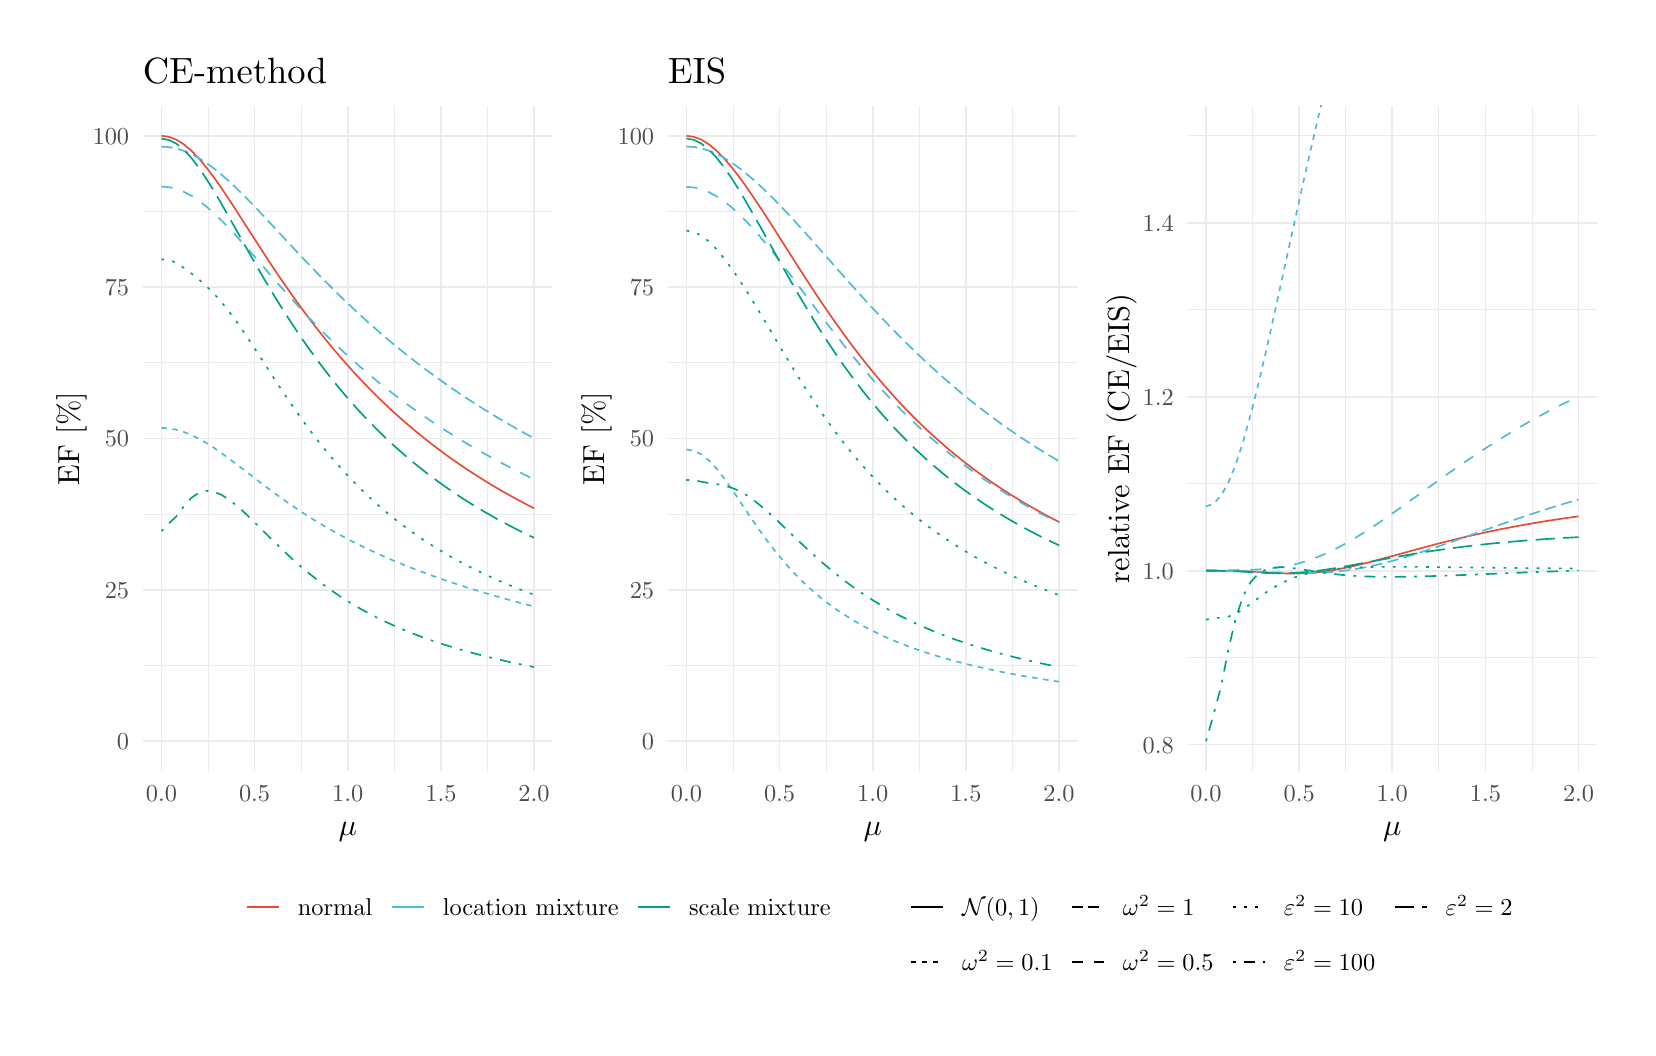
\begin{tikzpicture}[x=1pt,y=1pt]
\definecolor{fillColor}{RGB}{255,255,255}
\path[use as bounding box,fill=fillColor,fill opacity=0.00] (0,0) rectangle (578.16,361.35);
\begin{scope}
\path[clip] ( 41.61, 92.59) rectangle (189.71,333.19);
\definecolor{drawColor}{gray}{0.92}

\path[draw=drawColor,line width= 0.3pt,line join=round] ( 41.61,130.87) --
	(189.71,130.87);

\path[draw=drawColor,line width= 0.3pt,line join=round] ( 41.61,185.55) --
	(189.71,185.55);

\path[draw=drawColor,line width= 0.3pt,line join=round] ( 41.61,240.23) --
	(189.71,240.23);

\path[draw=drawColor,line width= 0.3pt,line join=round] ( 41.61,294.92) --
	(189.71,294.92);

\path[draw=drawColor,line width= 0.3pt,line join=round] ( 65.17, 92.59) --
	( 65.17,333.19);

\path[draw=drawColor,line width= 0.3pt,line join=round] ( 98.83, 92.59) --
	( 98.83,333.19);

\path[draw=drawColor,line width= 0.3pt,line join=round] (132.49, 92.59) --
	(132.49,333.19);

\path[draw=drawColor,line width= 0.3pt,line join=round] (166.14, 92.59) --
	(166.14,333.19);

\path[draw=drawColor,line width= 0.6pt,line join=round] ( 41.61,103.53) --
	(189.71,103.53);

\path[draw=drawColor,line width= 0.6pt,line join=round] ( 41.61,158.21) --
	(189.71,158.21);

\path[draw=drawColor,line width= 0.6pt,line join=round] ( 41.61,212.89) --
	(189.71,212.89);

\path[draw=drawColor,line width= 0.6pt,line join=round] ( 41.61,267.57) --
	(189.71,267.57);

\path[draw=drawColor,line width= 0.6pt,line join=round] ( 41.61,322.26) --
	(189.71,322.26);

\path[draw=drawColor,line width= 0.6pt,line join=round] ( 48.34, 92.59) --
	( 48.34,333.19);

\path[draw=drawColor,line width= 0.6pt,line join=round] ( 82.00, 92.59) --
	( 82.00,333.19);

\path[draw=drawColor,line width= 0.6pt,line join=round] (115.66, 92.59) --
	(115.66,333.19);

\path[draw=drawColor,line width= 0.6pt,line join=round] (149.32, 92.59) --
	(149.32,333.19);

\path[draw=drawColor,line width= 0.6pt,line join=round] (182.97, 92.59) --
	(182.97,333.19);
\definecolor{drawColor}{RGB}{230,75,53}

\path[draw=drawColor,line width= 0.6pt,line join=round] ( 48.34,322.26) --
	( 51.04,321.91) --
	( 53.73,320.87) --
	( 56.42,319.19) --
	( 59.11,316.93) --
	( 61.81,314.15) --
	( 64.50,310.94) --
	( 67.19,307.38) --
	( 69.88,303.57) --
	( 72.58,299.56) --
	( 75.27,295.44) --
	( 77.96,291.25) --
	( 80.65,287.04) --
	( 83.35,282.85) --
	( 86.04,278.70) --
	( 88.73,274.62) --
	( 91.42,270.62) --
	( 94.12,266.72) --
	( 96.81,262.92) --
	( 99.50,259.22) --
	(102.20,255.63) --
	(104.89,252.14) --
	(107.58,248.76) --
	(110.27,245.49) --
	(112.97,242.32) --
	(115.66,239.26) --
	(118.35,236.29) --
	(121.04,233.42) --
	(123.74,230.64) --
	(126.43,227.96) --
	(129.12,225.36) --
	(131.81,222.84) --
	(134.51,220.41) --
	(137.20,218.06) --
	(139.89,215.78) --
	(142.58,213.58) --
	(145.28,211.44) --
	(147.97,209.38) --
	(150.66,207.38) --
	(153.35,205.44) --
	(156.05,203.57) --
	(158.74,201.75) --
	(161.43,199.99) --
	(164.13,198.28) --
	(166.82,196.62) --
	(169.51,195.02) --
	(172.20,193.46) --
	(174.90,191.95) --
	(177.59,190.48) --
	(180.28,189.06) --
	(182.97,187.68);
\definecolor{drawColor}{RGB}{77,187,213}

\path[draw=drawColor,line width= 0.6pt,dash pattern=on 2pt off 2pt ,line join=round] ( 48.34,216.73) --
	( 51.04,216.56) --
	( 53.73,216.07) --
	( 56.42,215.28) --
	( 59.11,214.20) --
	( 61.81,212.87) --
	( 64.50,211.33) --
	( 67.19,209.60) --
	( 69.88,207.74) --
	( 72.58,205.78) --
	( 75.27,203.75) --
	( 77.96,201.69) --
	( 80.65,199.61) --
	( 83.35,197.54) --
	( 86.04,195.50) --
	( 88.73,193.49) --
	( 91.42,191.53) --
	( 94.12,189.63) --
	( 96.81,187.79) --
	( 99.50,186.00) --
	(102.20,184.28) --
	(104.89,182.62) --
	(107.58,181.02) --
	(110.27,179.48) --
	(112.97,177.99) --
	(115.66,176.56) --
	(118.35,175.18) --
	(121.04,173.84) --
	(123.74,172.55) --
	(126.43,171.31) --
	(129.12,170.11) --
	(131.81,168.94) --
	(134.51,167.81) --
	(137.20,166.72) --
	(139.89,165.66) --
	(142.58,164.64) --
	(145.28,163.64) --
	(147.97,162.67) --
	(150.66,161.73) --
	(153.35,160.81) --
	(156.05,159.92) --
	(158.74,159.06) --
	(161.43,158.22) --
	(164.13,157.40) --
	(166.82,156.60) --
	(169.51,155.82) --
	(172.20,155.06) --
	(174.90,154.32) --
	(177.59,153.60) --
	(180.28,152.89) --
	(182.97,152.21);

\path[draw=drawColor,line width= 0.6pt,dash pattern=on 4pt off 2pt ,line join=round] ( 48.34,318.36) --
	( 51.04,318.19) --
	( 53.73,317.68) --
	( 56.42,316.84) --
	( 59.11,315.68) --
	( 61.81,314.23) --
	( 64.50,312.51) --
	( 67.19,310.55) --
	( 69.88,308.37) --
	( 72.58,306.01) --
	( 75.27,303.50) --
	( 77.96,300.86) --
	( 80.65,298.12) --
	( 83.35,295.31) --
	( 86.04,292.45) --
	( 88.73,289.56) --
	( 91.42,286.66) --
	( 94.12,283.75) --
	( 96.81,280.87) --
	( 99.50,278.00) --
	(102.20,275.17) --
	(104.89,272.38) --
	(107.58,269.64) --
	(110.27,266.94) --
	(112.97,264.30) --
	(115.66,261.71) --
	(118.35,259.17) --
	(121.04,256.69) --
	(123.74,254.26) --
	(126.43,251.89) --
	(129.12,249.58) --
	(131.81,247.31) --
	(134.51,245.10) --
	(137.20,242.94) --
	(139.89,240.84) --
	(142.58,238.78) --
	(145.28,236.76) --
	(147.97,234.80) --
	(150.66,232.88) --
	(153.35,231.00) --
	(156.05,229.17) --
	(158.74,227.38) --
	(161.43,225.63) --
	(164.13,223.92) --
	(166.82,222.25) --
	(169.51,220.62) --
	(172.20,219.02) --
	(174.90,217.46) --
	(177.59,215.93) --
	(180.28,214.43) --
	(182.97,212.97);

\path[draw=drawColor,line width= 0.6pt,dash pattern=on 4pt off 4pt ,line join=round] ( 48.34,303.92) --
	( 51.04,303.71) --
	( 53.73,303.07) --
	( 56.42,302.03) --
	( 59.11,300.61) --
	( 61.81,298.84) --
	( 64.50,296.77) --
	( 67.19,294.42) --
	( 69.88,291.85) --
	( 72.58,289.10) --
	( 75.27,286.20) --
	( 77.96,283.21) --
	( 80.65,280.15) --
	( 83.35,277.05) --
	( 86.04,273.94) --
	( 88.73,270.84) --
	( 91.42,267.76) --
	( 94.12,264.73) --
	( 96.81,261.76) --
	( 99.50,258.84) --
	(102.20,255.99) --
	(104.89,253.21) --
	(107.58,250.49) --
	(110.27,247.86) --
	(112.97,245.29) --
	(115.66,242.80) --
	(118.35,240.37) --
	(121.04,238.02) --
	(123.74,235.73) --
	(126.43,233.50) --
	(129.12,231.34) --
	(131.81,229.24) --
	(134.51,227.19) --
	(137.20,225.20) --
	(139.89,223.26) --
	(142.58,221.38) --
	(145.28,219.54) --
	(147.97,217.75) --
	(150.66,216.01) --
	(153.35,214.31) --
	(156.05,212.66) --
	(158.74,211.04) --
	(161.43,209.47) --
	(164.13,207.93) --
	(166.82,206.43) --
	(169.51,204.97) --
	(172.20,203.54) --
	(174.90,202.15) --
	(177.59,200.79) --
	(180.28,199.46) --
	(182.97,198.15);
\definecolor{drawColor}{RGB}{0,160,135}

\path[draw=drawColor,line width= 0.6pt,dash pattern=on 1pt off 3pt ,line join=round] ( 48.34,277.59) --
	( 51.04,277.55) --
	( 53.73,276.30) --
	( 56.42,274.57) --
	( 59.11,272.59) --
	( 61.81,270.43) --
	( 64.50,268.04) --
	( 67.19,265.37) --
	( 69.88,262.36) --
	( 72.58,259.03) --
	( 75.27,255.40) --
	( 77.96,251.55) --
	( 80.65,247.52) --
	( 83.35,243.40) --
	( 86.04,239.24) --
	( 88.73,235.08) --
	( 91.42,230.98) --
	( 94.12,226.96) --
	( 96.81,223.05) --
	( 99.50,219.26) --
	(102.20,215.60) --
	(104.89,212.09) --
	(107.58,208.72) --
	(110.27,205.50) --
	(112.97,202.42) --
	(115.66,199.47) --
	(118.35,196.66) --
	(121.04,193.99) --
	(123.74,191.43) --
	(126.43,188.99) --
	(129.12,186.67) --
	(131.81,184.45) --
	(134.51,182.34) --
	(137.20,180.32) --
	(139.89,178.39) --
	(142.58,176.54) --
	(145.28,174.78) --
	(147.97,173.09) --
	(150.66,171.47) --
	(153.35,169.92) --
	(156.05,168.44) --
	(158.74,167.01) --
	(161.43,165.65) --
	(164.13,164.34) --
	(166.82,163.08) --
	(169.51,161.86) --
	(172.20,160.70) --
	(174.90,159.57) --
	(177.59,158.49) --
	(180.28,157.45) --
	(182.97,156.44);

\path[draw=drawColor,line width= 0.6pt,dash pattern=on 1pt off 3pt on 4pt off 3pt ,line join=round] ( 48.34,179.42) --
	( 51.04,182.21) --
	( 53.73,184.74) --
	( 56.42,188.36) --
	( 59.11,191.40) --
	( 61.81,193.27) --
	( 64.50,193.98) --
	( 67.19,193.69) --
	( 69.88,192.62) --
	( 72.58,190.95) --
	( 75.27,188.85) --
	( 77.96,186.47) --
	( 80.65,183.91) --
	( 83.35,181.25) --
	( 86.04,178.57) --
	( 88.73,175.90) --
	( 91.42,173.29) --
	( 94.12,170.75) --
	( 96.81,168.30) --
	( 99.50,165.96) --
	(102.20,163.72) --
	(104.89,161.59) --
	(107.58,159.57) --
	(110.27,157.65) --
	(112.97,155.83) --
	(115.66,154.10) --
	(118.35,152.47) --
	(121.04,150.93) --
	(123.74,149.47) --
	(126.43,148.08) --
	(129.12,146.77) --
	(131.81,145.52) --
	(134.51,144.34) --
	(137.20,143.21) --
	(139.89,142.15) --
	(142.58,141.13) --
	(145.28,140.16) --
	(147.97,139.24) --
	(150.66,138.36) --
	(153.35,137.52) --
	(156.05,136.72) --
	(158.74,135.95) --
	(161.43,135.22) --
	(164.13,134.52) --
	(166.82,133.84) --
	(169.51,133.20) --
	(172.20,132.58) --
	(174.90,131.98) --
	(177.59,131.41) --
	(180.28,130.86) --
	(182.97,130.33);

\path[draw=drawColor,line width= 0.6pt,dash pattern=on 7pt off 3pt ,line join=round] ( 48.34,321.24) --
	( 51.04,320.79) --
	( 53.73,319.43) --
	( 56.42,317.25) --
	( 59.11,314.34) --
	( 61.81,310.83) --
	( 64.50,306.84) --
	( 67.19,302.51) --
	( 69.88,297.94) --
	( 72.58,293.22) --
	( 75.27,288.43) --
	( 77.96,283.63) --
	( 80.65,278.86) --
	( 83.35,274.17) --
	( 86.04,269.56) --
	( 88.73,265.07) --
	( 91.42,260.71) --
	( 94.12,256.47) --
	( 96.81,252.37) --
	( 99.50,248.40) --
	(102.20,244.58) --
	(104.89,240.89) --
	(107.58,237.34) --
	(110.27,233.92) --
	(112.97,230.62) --
	(115.66,227.45) --
	(118.35,224.40) --
	(121.04,221.47) --
	(123.74,218.65) --
	(126.43,215.93) --
	(129.12,213.32) --
	(131.81,210.81) --
	(134.51,208.39) --
	(137.20,206.06) --
	(139.89,203.82) --
	(142.58,201.66) --
	(145.28,199.58) --
	(147.97,197.58) --
	(150.66,195.64) --
	(153.35,193.78) --
	(156.05,191.98) --
	(158.74,190.24) --
	(161.43,188.57) --
	(164.13,186.95) --
	(166.82,185.39) --
	(169.51,183.87) --
	(172.20,182.41) --
	(174.90,181.00) --
	(177.59,179.63) --
	(180.28,178.31) --
	(182.97,177.02);
\end{scope}
\begin{scope}
\path[clip] (  0.00,  0.00) rectangle (578.16,361.35);
\definecolor{drawColor}{gray}{0.30}

\node[text=drawColor,anchor=base east,inner sep=0pt, outer sep=0pt, scale=  0.88] at ( 36.66,100.50) {0};

\node[text=drawColor,anchor=base east,inner sep=0pt, outer sep=0pt, scale=  0.88] at ( 36.66,155.18) {25};

\node[text=drawColor,anchor=base east,inner sep=0pt, outer sep=0pt, scale=  0.88] at ( 36.66,209.86) {50};

\node[text=drawColor,anchor=base east,inner sep=0pt, outer sep=0pt, scale=  0.88] at ( 36.66,264.54) {75};

\node[text=drawColor,anchor=base east,inner sep=0pt, outer sep=0pt, scale=  0.88] at ( 36.66,319.23) {100};
\end{scope}
\begin{scope}
\path[clip] (  0.00,  0.00) rectangle (578.16,361.35);
\definecolor{drawColor}{gray}{0.30}

\node[text=drawColor,anchor=base,inner sep=0pt, outer sep=0pt, scale=  0.88] at ( 48.34, 81.58) {0.0};

\node[text=drawColor,anchor=base,inner sep=0pt, outer sep=0pt, scale=  0.88] at ( 82.00, 81.58) {0.5};

\node[text=drawColor,anchor=base,inner sep=0pt, outer sep=0pt, scale=  0.88] at (115.66, 81.58) {1.0};

\node[text=drawColor,anchor=base,inner sep=0pt, outer sep=0pt, scale=  0.88] at (149.32, 81.58) {1.5};

\node[text=drawColor,anchor=base,inner sep=0pt, outer sep=0pt, scale=  0.88] at (182.97, 81.58) {2.0};
\end{scope}
\begin{scope}
\path[clip] (  0.00,  0.00) rectangle (578.16,361.35);
\definecolor{drawColor}{RGB}{0,0,0}

\node[text=drawColor,anchor=base,inner sep=0pt, outer sep=0pt, scale=  1.10] at (115.66, 69.55) {$\mu$};
\end{scope}
\begin{scope}
\path[clip] (  0.00,  0.00) rectangle (578.16,361.35);
\definecolor{drawColor}{RGB}{0,0,0}

\node[text=drawColor,rotate= 90.00,anchor=base,inner sep=0pt, outer sep=0pt, scale=  1.10] at ( 18.58,212.89) {EF [\%]};
\end{scope}
\begin{scope}
\path[clip] (  0.00,  0.00) rectangle (578.16,361.35);
\definecolor{drawColor}{RGB}{0,0,0}

\node[text=drawColor,anchor=base west,inner sep=0pt, outer sep=0pt, scale=  1.32] at ( 41.61,341.26) {CE-method};
\end{scope}
\begin{scope}
\path[clip] (231.32, 92.59) rectangle (379.41,333.19);
\definecolor{drawColor}{gray}{0.92}

\path[draw=drawColor,line width= 0.3pt,line join=round] (231.32,130.87) --
	(379.41,130.87);

\path[draw=drawColor,line width= 0.3pt,line join=round] (231.32,185.55) --
	(379.41,185.55);

\path[draw=drawColor,line width= 0.3pt,line join=round] (231.32,240.23) --
	(379.41,240.23);

\path[draw=drawColor,line width= 0.3pt,line join=round] (231.32,294.92) --
	(379.41,294.92);

\path[draw=drawColor,line width= 0.3pt,line join=round] (254.88, 92.59) --
	(254.88,333.19);

\path[draw=drawColor,line width= 0.3pt,line join=round] (288.53, 92.59) --
	(288.53,333.19);

\path[draw=drawColor,line width= 0.3pt,line join=round] (322.19, 92.59) --
	(322.19,333.19);

\path[draw=drawColor,line width= 0.3pt,line join=round] (355.85, 92.59) --
	(355.85,333.19);

\path[draw=drawColor,line width= 0.6pt,line join=round] (231.32,103.53) --
	(379.41,103.53);

\path[draw=drawColor,line width= 0.6pt,line join=round] (231.32,158.21) --
	(379.41,158.21);

\path[draw=drawColor,line width= 0.6pt,line join=round] (231.32,212.89) --
	(379.41,212.89);

\path[draw=drawColor,line width= 0.6pt,line join=round] (231.32,267.57) --
	(379.41,267.57);

\path[draw=drawColor,line width= 0.6pt,line join=round] (231.32,322.26) --
	(379.41,322.26);

\path[draw=drawColor,line width= 0.6pt,line join=round] (238.05, 92.59) --
	(238.05,333.19);

\path[draw=drawColor,line width= 0.6pt,line join=round] (271.71, 92.59) --
	(271.71,333.19);

\path[draw=drawColor,line width= 0.6pt,line join=round] (305.36, 92.59) --
	(305.36,333.19);

\path[draw=drawColor,line width= 0.6pt,line join=round] (339.02, 92.59) --
	(339.02,333.19);

\path[draw=drawColor,line width= 0.6pt,line join=round] (372.68, 92.59) --
	(372.68,333.19);
\definecolor{drawColor}{RGB}{230,75,53}

\path[draw=drawColor,line width= 0.6pt,line join=round] (238.05,322.26) --
	(240.74,321.91) --
	(243.43,320.88) --
	(246.13,319.21) --
	(248.82,316.98) --
	(251.51,314.26) --
	(254.20,311.14) --
	(256.90,307.68) --
	(259.59,303.97) --
	(262.28,300.06) --
	(264.97,296.01) --
	(267.67,291.85) --
	(270.36,287.64) --
	(273.05,283.39) --
	(275.74,279.15) --
	(278.44,274.92) --
	(281.13,270.74) --
	(283.82,266.62) --
	(286.51,262.58) --
	(289.21,258.62) --
	(291.90,254.75) --
	(294.59,250.99) --
	(297.29,247.33) --
	(299.98,243.78) --
	(302.67,240.34) --
	(305.36,237.01) --
	(308.06,233.79) --
	(310.75,230.68) --
	(313.44,227.67) --
	(316.13,224.77) --
	(318.83,221.98) --
	(321.52,219.28) --
	(324.21,216.68) --
	(326.90,214.17) --
	(329.60,211.76) --
	(332.29,209.42) --
	(334.98,207.18) --
	(337.67,205.01) --
	(340.37,202.91) --
	(343.06,200.89) --
	(345.75,198.95) --
	(348.44,197.06) --
	(351.14,195.25) --
	(353.83,193.49) --
	(356.52,191.80) --
	(359.22,190.16) --
	(361.91,188.57) --
	(364.60,187.04) --
	(367.29,185.55) --
	(369.99,184.12) --
	(372.68,182.72);
\definecolor{drawColor}{RGB}{77,187,213}

\path[draw=drawColor,line width= 0.6pt,dash pattern=on 2pt off 2pt ,line join=round] (238.05,208.92) --
	(240.74,208.49) --
	(243.43,207.16) --
	(246.13,204.99) --
	(248.82,202.12) --
	(251.51,198.70) --
	(254.20,194.90) --
	(256.90,190.91) --
	(259.59,186.86) --
	(262.28,182.87) --
	(264.97,179.02) --
	(267.67,175.34) --
	(270.36,171.87) --
	(273.05,168.61) --
	(275.74,165.57) --
	(278.44,162.75) --
	(281.13,160.12) --
	(283.82,157.68) --
	(286.51,155.41) --
	(289.21,153.30) --
	(291.90,151.35) --
	(294.59,149.52) --
	(297.29,147.82) --
	(299.98,146.23) --
	(302.67,144.75) --
	(305.36,143.36) --
	(308.06,142.05) --
	(310.75,140.83) --
	(313.44,139.67) --
	(316.13,138.59) --
	(318.83,137.57) --
	(321.52,136.60) --
	(324.21,135.69) --
	(326.90,134.82) --
	(329.60,134.00) --
	(332.29,133.22) --
	(334.98,132.48) --
	(337.67,131.78) --
	(340.37,131.11) --
	(343.06,130.47) --
	(345.75,129.86) --
	(348.44,129.28) --
	(351.14,128.72) --
	(353.83,128.19) --
	(356.52,127.68) --
	(359.22,127.19) --
	(361.91,126.72) --
	(364.60,126.26) --
	(367.29,125.84) --
	(369.99,125.41) --
	(372.68,125.02);

\path[draw=drawColor,line width= 0.6pt,dash pattern=on 4pt off 2pt ,line join=round] (238.05,318.39) --
	(240.74,318.23) --
	(243.43,317.72) --
	(246.13,316.90) --
	(248.82,315.77) --
	(251.51,314.36) --
	(254.20,312.69) --
	(256.90,310.78) --
	(259.59,308.67) --
	(262.28,306.38) --
	(264.97,303.93) --
	(267.67,301.34) --
	(270.36,298.64) --
	(273.05,295.84) --
	(275.74,292.97) --
	(278.44,290.02) --
	(281.13,287.04) --
	(283.82,284.02) --
	(286.51,280.97) --
	(289.21,277.92) --
	(291.90,274.87) --
	(294.59,271.83) --
	(297.29,268.81) --
	(299.98,265.82) --
	(302.67,262.86) --
	(305.36,259.94) --
	(308.06,257.07) --
	(310.75,254.24) --
	(313.44,251.47) --
	(316.13,248.75) --
	(318.83,246.09) --
	(321.52,243.48) --
	(324.21,240.93) --
	(326.90,238.45) --
	(329.60,236.02) --
	(332.29,233.65) --
	(334.98,231.34) --
	(337.67,229.09) --
	(340.37,226.90) --
	(343.06,224.76) --
	(345.75,222.68) --
	(348.44,220.65) --
	(351.14,218.68) --
	(353.83,216.76) --
	(356.52,214.89) --
	(359.22,213.08) --
	(361.91,211.31) --
	(364.60,209.58) --
	(367.29,207.91) --
	(369.99,206.28) --
	(372.68,204.69);

\path[draw=drawColor,line width= 0.6pt,dash pattern=on 4pt off 4pt ,line join=round] (238.05,303.81) --
	(240.74,303.60) --
	(243.43,302.96) --
	(246.13,301.91) --
	(248.82,300.48) --
	(251.51,298.68) --
	(254.20,296.56) --
	(256.90,294.14) --
	(259.59,291.47) --
	(262.28,288.56) --
	(264.97,285.47) --
	(267.67,282.21) --
	(270.36,278.83) --
	(273.05,275.35) --
	(275.74,271.81) --
	(278.44,268.23) --
	(281.13,264.63) --
	(283.82,261.04) --
	(286.51,257.47) --
	(289.21,253.94) --
	(291.90,250.47) --
	(294.59,247.06) --
	(297.29,243.72) --
	(299.98,240.46) --
	(302.67,237.28) --
	(305.36,234.20) --
	(308.06,231.19) --
	(310.75,228.29) --
	(313.44,225.47) --
	(316.13,222.73) --
	(318.83,220.09) --
	(321.52,217.53) --
	(324.21,215.06) --
	(326.90,212.68) --
	(329.60,210.37) --
	(332.29,208.14) --
	(334.98,205.99) --
	(337.67,203.90) --
	(340.37,201.90) --
	(343.06,199.95) --
	(345.75,198.07) --
	(348.44,196.26) --
	(351.14,194.50) --
	(353.83,192.81) --
	(356.52,191.16) --
	(359.22,189.58) --
	(361.91,188.04) --
	(364.60,186.55) --
	(367.29,185.11) --
	(369.99,183.71) --
	(372.68,182.36);
\definecolor{drawColor}{RGB}{0,160,135}

\path[draw=drawColor,line width= 0.6pt,dash pattern=on 1pt off 3pt ,line join=round] (238.05,287.99) --
	(240.74,287.55) --
	(243.43,286.21) --
	(246.13,284.10) --
	(248.82,281.37) --
	(251.51,278.15) --
	(254.20,274.54) --
	(256.90,270.63) --
	(259.59,266.48) --
	(262.28,262.15) --
	(264.97,257.68) --
	(267.67,253.15) --
	(270.36,248.59) --
	(273.05,244.05) --
	(275.74,239.56) --
	(278.44,235.17) --
	(281.13,230.89) --
	(283.82,226.75) --
	(286.51,222.74) --
	(289.21,218.89) --
	(291.90,215.20) --
	(294.59,211.67) --
	(297.29,208.29) --
	(299.98,205.06) --
	(302.67,201.98) --
	(305.36,199.05) --
	(308.06,196.25) --
	(310.75,193.59) --
	(313.44,191.05) --
	(316.13,188.63) --
	(318.83,186.32) --
	(321.52,184.12) --
	(324.21,182.02) --
	(326.90,180.01) --
	(329.60,178.10) --
	(332.29,176.27) --
	(334.98,174.52) --
	(337.67,172.84) --
	(340.37,171.24) --
	(343.06,169.70) --
	(345.75,168.23) --
	(348.44,166.81) --
	(351.14,165.46) --
	(353.83,164.15) --
	(356.52,162.90) --
	(359.22,161.70) --
	(361.91,160.54) --
	(364.60,159.42) --
	(367.29,158.35) --
	(369.99,157.31) --
	(372.68,156.31);

\path[draw=drawColor,line width= 0.6pt,dash pattern=on 1pt off 3pt on 4pt off 3pt ,line join=round] (238.05,197.92) --
	(240.74,197.81) --
	(243.43,197.28) --
	(246.13,196.80) --
	(248.82,196.42) --
	(251.51,195.94) --
	(254.20,195.16) --
	(256.90,194.02) --
	(259.59,192.50) --
	(262.28,190.64) --
	(264.97,188.51) --
	(267.67,186.18) --
	(270.36,183.71) --
	(273.05,181.16) --
	(275.74,178.58) --
	(278.44,176.01) --
	(281.13,173.47) --
	(283.82,171.00) --
	(286.51,168.60) --
	(289.21,166.30) --
	(291.90,164.08) --
	(294.59,161.96) --
	(297.29,159.95) --
	(299.98,158.02) --
	(302.67,156.20) --
	(305.36,154.47) --
	(308.06,152.82) --
	(310.75,151.26) --
	(313.44,149.78) --
	(316.13,148.37) --
	(318.83,147.04) --
	(321.52,145.78) --
	(324.21,144.57) --
	(326.90,143.43) --
	(329.60,142.34) --
	(332.29,141.31) --
	(334.98,140.32) --
	(337.67,139.39) --
	(340.37,138.49) --
	(343.06,137.64) --
	(345.75,136.82) --
	(348.44,136.04) --
	(351.14,135.29) --
	(353.83,134.58) --
	(356.52,133.89) --
	(359.22,133.24) --
	(361.91,132.61) --
	(364.60,132.00) --
	(367.29,131.42) --
	(369.99,130.86) --
	(372.68,130.33);

\path[draw=drawColor,line width= 0.6pt,dash pattern=on 7pt off 3pt ,line join=round] (238.05,321.27) --
	(240.74,320.81) --
	(243.43,319.47) --
	(246.13,317.33) --
	(248.82,314.48) --
	(251.51,311.06) --
	(254.20,307.17) --
	(256.90,302.94) --
	(259.59,298.44) --
	(262.28,293.77) --
	(264.97,288.99) --
	(267.67,284.15) --
	(270.36,279.31) --
	(273.05,274.50) --
	(275.74,269.75) --
	(278.44,265.08) --
	(281.13,260.53) --
	(283.82,256.09) --
	(286.51,251.79) --
	(289.21,247.62) --
	(291.90,243.60) --
	(294.59,239.72) --
	(297.29,235.98) --
	(299.98,232.39) --
	(302.67,228.93) --
	(305.36,225.62) --
	(308.06,222.43) --
	(310.75,219.38) --
	(313.44,216.45) --
	(316.13,213.63) --
	(318.83,210.94) --
	(321.52,208.35) --
	(324.21,205.86) --
	(326.90,203.48) --
	(329.60,201.18) --
	(332.29,198.98) --
	(334.98,196.87) --
	(337.67,194.84) --
	(340.37,192.88) --
	(343.06,191.00) --
	(345.75,189.19) --
	(348.44,187.45) --
	(351.14,185.77) --
	(353.83,184.15) --
	(356.52,182.59) --
	(359.22,181.08) --
	(361.91,179.63) --
	(364.60,178.23) --
	(367.29,176.87) --
	(369.99,175.56) --
	(372.68,174.29);
\end{scope}
\begin{scope}
\path[clip] (  0.00,  0.00) rectangle (578.16,361.35);
\definecolor{drawColor}{gray}{0.30}

\node[text=drawColor,anchor=base east,inner sep=0pt, outer sep=0pt, scale=  0.88] at (226.37,100.50) {0};

\node[text=drawColor,anchor=base east,inner sep=0pt, outer sep=0pt, scale=  0.88] at (226.37,155.18) {25};

\node[text=drawColor,anchor=base east,inner sep=0pt, outer sep=0pt, scale=  0.88] at (226.37,209.86) {50};

\node[text=drawColor,anchor=base east,inner sep=0pt, outer sep=0pt, scale=  0.88] at (226.37,264.54) {75};

\node[text=drawColor,anchor=base east,inner sep=0pt, outer sep=0pt, scale=  0.88] at (226.37,319.23) {100};
\end{scope}
\begin{scope}
\path[clip] (  0.00,  0.00) rectangle (578.16,361.35);
\definecolor{drawColor}{gray}{0.30}

\node[text=drawColor,anchor=base,inner sep=0pt, outer sep=0pt, scale=  0.88] at (238.05, 81.58) {0.0};

\node[text=drawColor,anchor=base,inner sep=0pt, outer sep=0pt, scale=  0.88] at (271.71, 81.58) {0.5};

\node[text=drawColor,anchor=base,inner sep=0pt, outer sep=0pt, scale=  0.88] at (305.36, 81.58) {1.0};

\node[text=drawColor,anchor=base,inner sep=0pt, outer sep=0pt, scale=  0.88] at (339.02, 81.58) {1.5};

\node[text=drawColor,anchor=base,inner sep=0pt, outer sep=0pt, scale=  0.88] at (372.68, 81.58) {2.0};
\end{scope}
\begin{scope}
\path[clip] (  0.00,  0.00) rectangle (578.16,361.35);
\definecolor{drawColor}{RGB}{0,0,0}

\node[text=drawColor,anchor=base,inner sep=0pt, outer sep=0pt, scale=  1.10] at (305.36, 69.55) {$\mu$};
\end{scope}
\begin{scope}
\path[clip] (  0.00,  0.00) rectangle (578.16,361.35);
\definecolor{drawColor}{RGB}{0,0,0}

\node[text=drawColor,rotate= 90.00,anchor=base,inner sep=0pt, outer sep=0pt, scale=  1.10] at (208.28,212.89) {EF [\%]};
\end{scope}
\begin{scope}
\path[clip] (  0.00,  0.00) rectangle (578.16,361.35);
\definecolor{drawColor}{RGB}{0,0,0}

\node[text=drawColor,anchor=base west,inner sep=0pt, outer sep=0pt, scale=  1.32] at (231.32,341.26) {EIS};
\end{scope}
\begin{scope}
\path[clip] (419.07, 92.59) rectangle (567.16,333.19);
\definecolor{drawColor}{gray}{0.92}

\path[draw=drawColor,line width= 0.3pt,line join=round] (419.07,133.70) --
	(567.16,133.70);

\path[draw=drawColor,line width= 0.3pt,line join=round] (419.07,196.55) --
	(567.16,196.55);

\path[draw=drawColor,line width= 0.3pt,line join=round] (419.07,259.40) --
	(567.16,259.40);

\path[draw=drawColor,line width= 0.3pt,line join=round] (419.07,322.26) --
	(567.16,322.26);

\path[draw=drawColor,line width= 0.3pt,line join=round] (442.63, 92.59) --
	(442.63,333.19);

\path[draw=drawColor,line width= 0.3pt,line join=round] (476.28, 92.59) --
	(476.28,333.19);

\path[draw=drawColor,line width= 0.3pt,line join=round] (509.94, 92.59) --
	(509.94,333.19);

\path[draw=drawColor,line width= 0.3pt,line join=round] (543.60, 92.59) --
	(543.60,333.19);

\path[draw=drawColor,line width= 0.6pt,line join=round] (419.07,102.27) --
	(567.16,102.27);

\path[draw=drawColor,line width= 0.6pt,line join=round] (419.07,165.12) --
	(567.16,165.12);

\path[draw=drawColor,line width= 0.6pt,line join=round] (419.07,227.98) --
	(567.16,227.98);

\path[draw=drawColor,line width= 0.6pt,line join=round] (419.07,290.83) --
	(567.16,290.83);

\path[draw=drawColor,line width= 0.6pt,line join=round] (425.80, 92.59) --
	(425.80,333.19);

\path[draw=drawColor,line width= 0.6pt,line join=round] (459.46, 92.59) --
	(459.46,333.19);

\path[draw=drawColor,line width= 0.6pt,line join=round] (493.11, 92.59) --
	(493.11,333.19);

\path[draw=drawColor,line width= 0.6pt,line join=round] (526.77, 92.59) --
	(526.77,333.19);

\path[draw=drawColor,line width= 0.6pt,line join=round] (560.43, 92.59) --
	(560.43,333.19);
\definecolor{drawColor}{RGB}{230,75,53}

\path[draw=drawColor,line width= 0.6pt,line join=round] (425.80,165.12) --
	(428.49,165.12) --
	(431.18,165.12) --
	(433.88,165.10) --
	(436.57,165.04) --
	(439.26,164.95) --
	(441.95,164.82) --
	(444.65,164.66) --
	(447.34,164.49) --
	(450.03,164.33) --
	(452.72,164.19) --
	(455.42,164.11) --
	(458.11,164.10) --
	(460.80,164.17) --
	(463.49,164.33) --
	(466.19,164.57) --
	(468.88,164.90) --
	(471.57,165.31) --
	(474.26,165.80) --
	(476.96,166.34) --
	(479.65,166.94) --
	(482.34,167.58) --
	(485.04,168.26) --
	(487.73,168.97) --
	(490.42,169.69) --
	(493.11,170.42) --
	(495.81,171.16) --
	(498.50,171.90) --
	(501.19,172.64) --
	(503.88,173.37) --
	(506.58,174.09) --
	(509.27,174.80) --
	(511.96,175.49) --
	(514.65,176.16) --
	(517.35,176.81) --
	(520.04,177.45) --
	(522.73,178.07) --
	(525.42,178.67) --
	(528.12,179.25) --
	(530.81,179.81) --
	(533.50,180.35) --
	(536.19,180.87) --
	(538.89,181.37) --
	(541.58,181.85) --
	(544.27,182.32) --
	(546.97,182.77) --
	(549.66,183.20) --
	(552.35,183.62) --
	(555.04,184.02) --
	(557.74,184.40) --
	(560.43,184.77);
\definecolor{drawColor}{RGB}{77,187,213}

\path[draw=drawColor,line width= 0.6pt,dash pattern=on 2pt off 2pt ,line join=round] (425.80,188.40) --
	(428.49,189.29) --
	(431.18,192.17) --
	(433.88,196.98) --
	(436.57,203.63) --
	(439.26,211.93) --
	(441.95,221.60) --
	(444.65,232.35) --
	(447.34,243.86) --
	(450.03,255.86) --
	(452.72,268.11) --
	(455.42,280.44) --
	(458.11,292.70) --
	(460.80,304.82) --
	(463.49,316.68) --
	(466.19,328.29) --
	(468.88,339.58) --
	(471.57,350.57) --
	(474.26,361.23) --
	(476.96,371.58) --
	(479.65,381.61) --
	(482.34,391.32) --
	(485.04,400.71) --
	(487.73,409.83) --
	(490.42,418.62) --
	(493.11,427.13) --
	(495.81,435.33) --
	(498.50,443.27) --
	(501.19,451.00) --
	(503.88,458.41) --
	(506.58,465.52) --
	(509.27,472.43) --
	(511.96,479.03) --
	(514.65,485.44) --
	(517.35,491.62) --
	(520.04,497.59) --
	(522.73,503.30) --
	(525.42,508.74) --
	(528.12,514.01) --
	(530.81,519.13) --
	(533.50,524.04) --
	(536.19,528.56) --
	(538.89,533.09) --
	(541.58,537.38) --
	(544.27,541.48) --
	(546.97,545.45) --
	(549.66,549.09) --
	(552.35,552.97) --
	(555.04,555.99) --
	(557.74,559.72) --
	(560.43,562.80);

\path[draw=drawColor,line width= 0.6pt,dash pattern=on 4pt off 2pt ,line join=round] (425.80,165.08) --
	(428.49,165.07) --
	(431.18,165.06) --
	(433.88,165.03) --
	(436.57,164.99) --
	(439.26,164.94) --
	(441.95,164.86) --
	(444.65,164.77) --
	(447.34,164.66) --
	(450.03,164.55) --
	(452.72,164.45) --
	(455.42,164.36) --
	(458.11,164.29) --
	(460.80,164.26) --
	(463.49,164.27) --
	(466.19,164.34) --
	(468.88,164.47) --
	(471.57,164.67) --
	(474.26,164.94) --
	(476.96,165.28) --
	(479.65,165.68) --
	(482.34,166.16) --
	(485.04,166.70) --
	(487.73,167.30) --
	(490.42,167.96) --
	(493.11,168.67) --
	(495.81,169.43) --
	(498.50,170.23) --
	(501.19,171.06) --
	(503.88,171.92) --
	(506.58,172.82) --
	(509.27,173.73) --
	(511.96,174.66) --
	(514.65,175.60) --
	(517.35,176.55) --
	(520.04,177.51) --
	(522.73,178.46) --
	(525.42,179.42) --
	(528.12,180.37) --
	(530.81,181.31) --
	(533.50,182.25) --
	(536.19,183.18) --
	(538.89,184.09) --
	(541.58,185.00) --
	(544.27,185.89) --
	(546.97,186.76) --
	(549.66,187.61) --
	(552.35,188.45) --
	(555.04,189.28) --
	(557.74,190.08) --
	(560.43,190.87);

\path[draw=drawColor,line width= 0.6pt,dash pattern=on 4pt off 4pt ,line join=round] (425.80,165.29) --
	(428.49,165.30) --
	(431.18,165.30) --
	(433.88,165.32) --
	(436.57,165.34) --
	(439.26,165.39) --
	(441.95,165.46) --
	(444.65,165.58) --
	(447.34,165.77) --
	(450.03,166.04) --
	(452.72,166.40) --
	(455.42,166.88) --
	(458.11,167.49) --
	(460.80,168.23) --
	(463.49,169.10) --
	(466.19,170.11) --
	(468.88,171.24) --
	(471.57,172.50) --
	(474.26,173.88) --
	(476.96,175.36) --
	(479.65,176.93) --
	(482.34,178.59) --
	(485.04,180.31) --
	(487.73,182.10) --
	(490.42,183.94) --
	(493.11,185.81) --
	(495.81,187.72) --
	(498.50,189.64) --
	(501.19,191.57) --
	(503.88,193.51) --
	(506.58,195.45) --
	(509.27,197.38) --
	(511.96,199.29) --
	(514.65,201.19) --
	(517.35,203.05) --
	(520.04,204.90) --
	(522.73,206.70) --
	(525.42,208.49) --
	(528.12,210.22) --
	(530.81,211.94) --
	(533.50,213.61) --
	(536.19,215.24) --
	(538.89,216.83) --
	(541.58,218.38) --
	(544.27,219.89) --
	(546.97,221.36) --
	(549.66,222.79) --
	(552.35,224.17) --
	(555.04,225.52) --
	(557.74,226.83) --
	(560.43,228.10);
\definecolor{drawColor}{RGB}{0,160,135}

\path[draw=drawColor,line width= 0.6pt,dash pattern=on 1pt off 3pt ,line join=round] (425.80,147.41) --
	(428.49,148.05) --
	(431.18,148.08) --
	(433.88,148.53) --
	(436.57,149.60) --
	(439.26,151.23) --
	(441.95,153.18) --
	(444.65,155.22) --
	(447.34,157.18) --
	(450.03,158.94) --
	(452.72,160.47) --
	(455.42,161.76) --
	(458.11,162.82) --
	(460.80,163.68) --
	(463.49,164.37) --
	(466.19,164.91) --
	(468.88,165.34) --
	(471.57,165.67) --
	(474.26,165.92) --
	(476.96,166.12) --
	(479.65,166.26) --
	(482.34,166.36) --
	(485.04,166.43) --
	(487.73,166.48) --
	(490.42,166.51) --
	(493.11,166.52) --
	(495.81,166.52) --
	(498.50,166.51) --
	(501.19,166.50) --
	(503.88,166.48) --
	(506.58,166.46) --
	(509.27,166.43) --
	(511.96,166.40) --
	(514.65,166.37) --
	(517.35,166.34) --
	(520.04,166.31) --
	(522.73,166.28) --
	(525.42,166.25) --
	(528.12,166.22) --
	(530.81,166.19) --
	(533.50,166.16) --
	(536.19,166.13) --
	(538.89,166.10) --
	(541.58,166.07) --
	(544.27,166.05) --
	(546.97,166.02) --
	(549.66,166.00) --
	(552.35,165.97) --
	(555.04,165.95) --
	(557.74,165.93) --
	(560.43,165.90);

\path[draw=drawColor,line width= 0.6pt,dash pattern=on 1pt off 3pt on 4pt off 3pt ,line join=round] (425.80,103.53) --
	(428.49,113.12) --
	(431.18,123.09) --
	(433.88,136.69) --
	(436.57,148.14) --
	(439.26,156.07) --
	(441.95,161.07) --
	(444.65,163.98) --
	(447.34,165.54) --
	(450.03,166.23) --
	(452.72,166.39) --
	(455.42,166.24) --
	(458.11,165.92) --
	(460.80,165.52) --
	(463.49,165.09) --
	(466.19,164.67) --
	(468.88,164.29) --
	(471.57,163.96) --
	(474.26,163.67) --
	(476.96,163.44) --
	(479.65,163.25) --
	(482.34,163.11) --
	(485.04,163.01) --
	(487.73,162.94) --
	(490.42,162.91) --
	(493.11,162.90) --
	(495.81,162.91) --
	(498.50,162.95) --
	(501.19,163.00) --
	(503.88,163.07) --
	(506.58,163.14) --
	(509.27,163.23) --
	(511.96,163.32) --
	(514.65,163.42) --
	(517.35,163.52) --
	(520.04,163.63) --
	(522.73,163.74) --
	(525.42,163.85) --
	(528.12,163.96) --
	(530.81,164.07) --
	(533.50,164.17) --
	(536.19,164.28) --
	(538.89,164.39) --
	(541.58,164.50) --
	(544.27,164.60) --
	(546.97,164.70) --
	(549.66,164.80) --
	(552.35,164.90) --
	(555.04,165.00) --
	(557.74,165.10) --
	(560.43,165.19);

\path[draw=drawColor,line width= 0.6pt,dash pattern=on 7pt off 3pt ,line join=round] (425.80,165.08) --
	(428.49,165.09) --
	(431.18,165.06) --
	(433.88,165.00) --
	(436.57,164.91) --
	(439.26,164.77) --
	(441.95,164.61) --
	(444.65,164.45) --
	(447.34,164.31) --
	(450.03,164.22) --
	(452.72,164.18) --
	(455.42,164.22) --
	(458.11,164.33) --
	(460.80,164.52) --
	(463.49,164.78) --
	(466.19,165.10) --
	(468.88,165.48) --
	(471.57,165.90) --
	(474.26,166.35) --
	(476.96,166.83) --
	(479.65,167.33) --
	(482.34,167.84) --
	(485.04,168.34) --
	(487.73,168.85) --
	(490.42,169.35) --
	(493.11,169.85) --
	(495.81,170.33) --
	(498.50,170.80) --
	(501.19,171.25) --
	(503.88,171.69) --
	(506.58,172.11) --
	(509.27,172.51) --
	(511.96,172.89) --
	(514.65,173.26) --
	(517.35,173.61) --
	(520.04,173.94) --
	(522.73,174.26) --
	(525.42,174.56) --
	(528.12,174.84) --
	(530.81,175.11) --
	(533.50,175.36) --
	(536.19,175.60) --
	(538.89,175.83) --
	(541.58,176.05) --
	(544.27,176.25) --
	(546.97,176.44) --
	(549.66,176.63) --
	(552.35,176.79) --
	(555.04,176.96) --
	(557.74,177.11) --
	(560.43,177.25);
\end{scope}
\begin{scope}
\path[clip] (  0.00,  0.00) rectangle (578.16,361.35);
\definecolor{drawColor}{gray}{0.30}

\node[text=drawColor,anchor=base east,inner sep=0pt, outer sep=0pt, scale=  0.88] at (414.12, 99.24) {0.8};

\node[text=drawColor,anchor=base east,inner sep=0pt, outer sep=0pt, scale=  0.88] at (414.12,162.09) {1.0};

\node[text=drawColor,anchor=base east,inner sep=0pt, outer sep=0pt, scale=  0.88] at (414.12,224.95) {1.2};

\node[text=drawColor,anchor=base east,inner sep=0pt, outer sep=0pt, scale=  0.88] at (414.12,287.80) {1.4};
\end{scope}
\begin{scope}
\path[clip] (  0.00,  0.00) rectangle (578.16,361.35);
\definecolor{drawColor}{gray}{0.30}

\node[text=drawColor,anchor=base,inner sep=0pt, outer sep=0pt, scale=  0.88] at (425.80, 81.58) {0.0};

\node[text=drawColor,anchor=base,inner sep=0pt, outer sep=0pt, scale=  0.88] at (459.46, 81.58) {0.5};

\node[text=drawColor,anchor=base,inner sep=0pt, outer sep=0pt, scale=  0.88] at (493.11, 81.58) {1.0};

\node[text=drawColor,anchor=base,inner sep=0pt, outer sep=0pt, scale=  0.88] at (526.77, 81.58) {1.5};

\node[text=drawColor,anchor=base,inner sep=0pt, outer sep=0pt, scale=  0.88] at (560.43, 81.58) {2.0};
\end{scope}
\begin{scope}
\path[clip] (  0.00,  0.00) rectangle (578.16,361.35);
\definecolor{drawColor}{RGB}{0,0,0}

\node[text=drawColor,anchor=base,inner sep=0pt, outer sep=0pt, scale=  1.10] at (493.11, 69.55) {$\mu$};
\end{scope}
\begin{scope}
\path[clip] (  0.00,  0.00) rectangle (578.16,361.35);
\definecolor{drawColor}{RGB}{0,0,0}

\node[text=drawColor,rotate= 90.00,anchor=base,inner sep=0pt, outer sep=0pt, scale=  1.10] at (397.99,212.89) {relative EF (CE/EIS)};
\end{scope}
\begin{scope}
\path[clip] (  0.00,  0.00) rectangle (578.16,361.35);
\definecolor{drawColor}{RGB}{230,75,53}

\path[draw=drawColor,line width= 0.6pt,line join=round] ( 79.13, 43.68) -- ( 90.69, 43.68);
\end{scope}
\begin{scope}
\path[clip] (  0.00,  0.00) rectangle (578.16,361.35);
\definecolor{drawColor}{RGB}{77,187,213}

\path[draw=drawColor,line width= 0.6pt,line join=round] (131.49, 43.68) -- (143.05, 43.68);
\end{scope}
\begin{scope}
\path[clip] (  0.00,  0.00) rectangle (578.16,361.35);
\definecolor{drawColor}{RGB}{0,160,135}

\path[draw=drawColor,line width= 0.6pt,line join=round] (220.51, 43.68) -- (232.07, 43.68);
\end{scope}
\begin{scope}
\path[clip] (  0.00,  0.00) rectangle (578.16,361.35);
\definecolor{drawColor}{RGB}{0,0,0}

\node[text=drawColor,anchor=base west,inner sep=0pt, outer sep=0pt, scale=  0.88] at ( 97.64, 40.65) {normal};
\end{scope}
\begin{scope}
\path[clip] (  0.00,  0.00) rectangle (578.16,361.35);
\definecolor{drawColor}{RGB}{0,0,0}

\node[text=drawColor,anchor=base west,inner sep=0pt, outer sep=0pt, scale=  0.88] at (150.00, 40.65) {location mixture};
\end{scope}
\begin{scope}
\path[clip] (  0.00,  0.00) rectangle (578.16,361.35);
\definecolor{drawColor}{RGB}{0,0,0}

\node[text=drawColor,anchor=base west,inner sep=0pt, outer sep=0pt, scale=  0.88] at (239.02, 40.65) {scale mixture};
\end{scope}
\begin{scope}
\path[clip] (  0.00,  0.00) rectangle (578.16,361.35);
\definecolor{drawColor}{RGB}{0,0,0}

\path[draw=drawColor,line width= 0.6pt,line join=round] (319.11, 43.68) -- (330.67, 43.68);
\end{scope}
\begin{scope}
\path[clip] (  0.00,  0.00) rectangle (578.16,361.35);
\definecolor{drawColor}{RGB}{0,0,0}

\path[draw=drawColor,line width= 0.6pt,dash pattern=on 2pt off 2pt ,line join=round] (319.11, 23.73) -- (330.67, 23.73);
\end{scope}
\begin{scope}
\path[clip] (  0.00,  0.00) rectangle (578.16,361.35);
\definecolor{drawColor}{RGB}{0,0,0}

\path[draw=drawColor,line width= 0.6pt,dash pattern=on 4pt off 2pt ,line join=round] (377.28, 43.68) -- (388.85, 43.68);
\end{scope}
\begin{scope}
\path[clip] (  0.00,  0.00) rectangle (578.16,361.35);
\definecolor{drawColor}{RGB}{0,0,0}

\path[draw=drawColor,line width= 0.6pt,dash pattern=on 4pt off 4pt ,line join=round] (377.28, 23.73) -- (388.85, 23.73);
\end{scope}
\begin{scope}
\path[clip] (  0.00,  0.00) rectangle (578.16,361.35);
\definecolor{drawColor}{RGB}{0,0,0}

\path[draw=drawColor,line width= 0.6pt,dash pattern=on 1pt off 3pt ,line join=round] (435.46, 43.68) -- (447.02, 43.68);
\end{scope}
\begin{scope}
\path[clip] (  0.00,  0.00) rectangle (578.16,361.35);
\definecolor{drawColor}{RGB}{0,0,0}

\path[draw=drawColor,line width= 0.6pt,dash pattern=on 1pt off 3pt on 4pt off 3pt ,line join=round] (435.46, 23.73) -- (447.02, 23.73);
\end{scope}
\begin{scope}
\path[clip] (  0.00,  0.00) rectangle (578.16,361.35);
\definecolor{drawColor}{RGB}{0,0,0}

\path[draw=drawColor,line width= 0.6pt,dash pattern=on 7pt off 3pt ,line join=round] (493.90, 43.68) -- (505.46, 43.68);
\end{scope}
\begin{scope}
\path[clip] (  0.00,  0.00) rectangle (578.16,361.35);
\definecolor{drawColor}{RGB}{0,0,0}

\node[text=drawColor,anchor=base west,inner sep=0pt, outer sep=0pt, scale=  0.88] at (337.62, 40.65) {$\mathcal N (0, 1)$};
\end{scope}
\begin{scope}
\path[clip] (  0.00,  0.00) rectangle (578.16,361.35);
\definecolor{drawColor}{RGB}{0,0,0}

\node[text=drawColor,anchor=base west,inner sep=0pt, outer sep=0pt, scale=  0.88] at (337.62, 20.70) {$\omega^2 = 0.1$};
\end{scope}
\begin{scope}
\path[clip] (  0.00,  0.00) rectangle (578.16,361.35);
\definecolor{drawColor}{RGB}{0,0,0}

\node[text=drawColor,anchor=base west,inner sep=0pt, outer sep=0pt, scale=  0.88] at (395.79, 40.65) {$\omega^2 = 1$};
\end{scope}
\begin{scope}
\path[clip] (  0.00,  0.00) rectangle (578.16,361.35);
\definecolor{drawColor}{RGB}{0,0,0}

\node[text=drawColor,anchor=base west,inner sep=0pt, outer sep=0pt, scale=  0.88] at (395.79, 20.70) {$\omega^2= 0.5$};
\end{scope}
\begin{scope}
\path[clip] (  0.00,  0.00) rectangle (578.16,361.35);
\definecolor{drawColor}{RGB}{0,0,0}

\node[text=drawColor,anchor=base west,inner sep=0pt, outer sep=0pt, scale=  0.88] at (453.97, 40.65) {$\varepsilon^2 = 10$};
\end{scope}
\begin{scope}
\path[clip] (  0.00,  0.00) rectangle (578.16,361.35);
\definecolor{drawColor}{RGB}{0,0,0}

\node[text=drawColor,anchor=base west,inner sep=0pt, outer sep=0pt, scale=  0.88] at (453.97, 20.70) {$\varepsilon^2 = 100$};
\end{scope}
\begin{scope}
\path[clip] (  0.00,  0.00) rectangle (578.16,361.35);
\definecolor{drawColor}{RGB}{0,0,0}

\node[text=drawColor,anchor=base west,inner sep=0pt, outer sep=0pt, scale=  0.88] at (512.40, 40.65) {$\varepsilon^2 = 2$};
\end{scope}
\end{tikzpicture}
%
    }
    \caption{{\color{red} TODO}}
    \label{fig:rho}
\end{figure} 

In this figure, we can observe that, as expected, misspecification in $\mu$ almost always results in a smaller efficiency factor, an exception being the scale mixture with $\varepsilon^{2} = 100$ for the \acem. 
Compared to \Cref{fig:rho_mu}, we see that already small misspecification in $\mu$ results in a large decline in EF, although we should keep in mind that this is not a fair comparison, as $\mu$ and $\sigma^{2}$ live on different scales.
If $\mu = 0 $ is correctly specified, both methods have comparable performance, except for extreme cases of the mixture models, i.e. when $\omega^{2} = 0.1$ or when $\varepsilon^{2} = 100$. 
For small misspecification of $\mu$, this remains true, but for larger misspecification, the \acem has a larger efficiency factor, especially for the bimodal location mixture with $\omega^{2} = 0.1$, where the performance of \aeis deteriorates. 

\todo{stress that cem gives global optimum, eis only approximate}

%% rho
For the model from \Cref{ex:negbinom-ar1} we cannot determine $\rho$ analytically, so we fall back to a simulation study.
Thus, we also estimate $\text{EF}$ for each of the $M$ runs, using the same number of samples $N = N_{\text{true}}$ as was used to determine the true optimal parameter.
We display the resulting efficiency factors in \Cref{fig:ef_time_dimension}. The parameters $\alpha, r, N, M$ may be found in the bottom right corner of the figure.
For a low number of time steps $n$, all three methods perform comparably. With increasing $n$, their performance expectedly worsens, however, more so for the local \gls{la}, while the \gls{cem} and \gls{eis} perform comparably around their optimal value. 

\begin{figure}
    \resizebox{\textwidth}{!}{%
        % Created by tikzDevice version 0.12.6 on 2024-05-22 15:03:06
% !TEX encoding = UTF-8 Unicode
\begin{tikzpicture}[x=1pt,y=1pt]
\definecolor{fillColor}{RGB}{255,255,255}
\path[use as bounding box,fill=fillColor,fill opacity=0.00] (0,0) rectangle (578.16,361.35);
\begin{scope}
\path[clip] ( 36.11, 30.69) rectangle (514.31,355.85);
\definecolor{drawColor}{gray}{0.92}

\path[draw=drawColor,line width= 0.3pt,line join=round] ( 36.11, 61.66) --
	(514.31, 61.66);

\path[draw=drawColor,line width= 0.3pt,line join=round] ( 36.11,141.63) --
	(514.31,141.63);

\path[draw=drawColor,line width= 0.3pt,line join=round] ( 36.11,221.60) --
	(514.31,221.60);

\path[draw=drawColor,line width= 0.3pt,line join=round] ( 36.11,301.57) --
	(514.31,301.57);

\path[draw=drawColor,line width= 0.3pt,line join=round] (157.33, 30.69) --
	(157.33,355.85);

\path[draw=drawColor,line width= 0.3pt,line join=round] (300.40, 30.69) --
	(300.40,355.85);

\path[draw=drawColor,line width= 0.3pt,line join=round] (443.47, 30.69) --
	(443.47,355.85);

\path[draw=drawColor,line width= 0.6pt,line join=round] ( 36.11,101.64) --
	(514.31,101.64);

\path[draw=drawColor,line width= 0.6pt,line join=round] ( 36.11,181.61) --
	(514.31,181.61);

\path[draw=drawColor,line width= 0.6pt,line join=round] ( 36.11,261.59) --
	(514.31,261.59);

\path[draw=drawColor,line width= 0.6pt,line join=round] ( 36.11,341.56) --
	(514.31,341.56);

\path[draw=drawColor,line width= 0.6pt,line join=round] ( 89.07, 30.69) --
	( 89.07,355.85);

\path[draw=drawColor,line width= 0.6pt,line join=round] (225.59, 30.69) --
	(225.59,355.85);

\path[draw=drawColor,line width= 0.6pt,line join=round] (375.21, 30.69) --
	(375.21,355.85);

\path[draw=drawColor,line width= 0.6pt,line join=round] (511.73, 30.69) --
	(511.73,355.85);
\definecolor{drawColor}{RGB}{230,75,53}

\path[draw=drawColor,line width= 0.6pt,line join=round] ( 67.54,340.90) -- ( 67.54,341.06);

\path[draw=drawColor,line width= 0.6pt,line join=round] ( 67.54,340.59) -- ( 67.54,340.43);
\definecolor{fillColor}{RGB}{255,255,255}

\path[draw=drawColor,line width= 0.6pt,line join=round,line cap=round,fill=fillColor] ( 57.85,340.90) --
	( 57.85,340.59) --
	( 77.23,340.59) --
	( 77.23,340.90) --
	( 57.85,340.90) --
	cycle;

\path[draw=drawColor,line width= 1.1pt,line join=round] ( 57.85,340.74) -- ( 77.23,340.74);

\path[draw=drawColor,line width= 0.6pt,line join=round] (153.67,337.06) -- (153.67,338.93);

\path[draw=drawColor,line width= 0.6pt,line join=round] (153.67,333.31) -- (153.67,331.44);

\path[draw=drawColor,line width= 0.6pt,line join=round,line cap=round,fill=fillColor] (143.98,337.06) --
	(143.98,333.31) --
	(163.36,333.31) --
	(163.36,337.06) --
	(143.98,337.06) --
	cycle;

\path[draw=drawColor,line width= 1.1pt,line join=round] (143.98,335.18) -- (163.36,335.18);

\path[draw=drawColor,line width= 0.6pt,line join=round] (267.54,326.01) -- (267.54,326.91);

\path[draw=drawColor,line width= 0.6pt,line join=round] (267.54,324.21) -- (267.54,323.31);

\path[draw=drawColor,line width= 0.6pt,line join=round,line cap=round,fill=fillColor] (257.85,326.01) --
	(257.85,324.21) --
	(277.23,324.21) --
	(277.23,326.01) --
	(257.85,326.01) --
	cycle;

\path[draw=drawColor,line width= 1.1pt,line join=round] (257.85,325.11) -- (277.23,325.11);

\path[draw=drawColor,line width= 0.6pt,line join=round] (353.68,318.44) -- (353.68,320.87);

\path[draw=drawColor,line width= 0.6pt,line join=round] (353.68,313.56) -- (353.68,311.13);

\path[draw=drawColor,line width= 0.6pt,line join=round,line cap=round,fill=fillColor] (343.99,318.44) --
	(343.99,313.56) --
	(363.37,313.56) --
	(363.37,318.44) --
	(343.99,318.44) --
	cycle;

\path[draw=drawColor,line width= 1.1pt,line join=round] (343.99,316.00) -- (363.37,316.00);

\path[draw=drawColor,line width= 0.6pt,line join=round] (439.81,253.60) -- (439.81,258.34);

\path[draw=drawColor,line width= 0.6pt,line join=round] (439.81,244.13) -- (439.81,239.39);

\path[draw=drawColor,line width= 0.6pt,line join=round,line cap=round,fill=fillColor] (430.12,253.60) --
	(430.12,244.13) --
	(449.50,244.13) --
	(449.50,253.60) --
	(430.12,253.60) --
	cycle;

\path[draw=drawColor,line width= 1.1pt,line join=round] (430.12,248.87) -- (449.50,248.87);
\definecolor{drawColor}{RGB}{77,187,213}

\path[draw=drawColor,line width= 0.6pt,line join=round] ( 89.07,340.92) -- ( 89.07,341.07);

\path[draw=drawColor,line width= 0.6pt,line join=round] ( 89.07,340.61) -- ( 89.07,340.46);

\path[draw=drawColor,line width= 0.6pt,line join=round,line cap=round,fill=fillColor] ( 79.38,340.92) --
	( 79.38,340.61) --
	( 98.76,340.61) --
	( 98.76,340.92) --
	( 79.38,340.92) --
	cycle;

\path[draw=drawColor,line width= 1.1pt,line join=round] ( 79.38,340.77) -- ( 98.76,340.77);

\path[draw=drawColor,line width= 0.6pt,line join=round] (175.21,337.10) -- (175.21,338.97);

\path[draw=drawColor,line width= 0.6pt,line join=round] (175.21,333.35) -- (175.21,331.48);

\path[draw=drawColor,line width= 0.6pt,line join=round,line cap=round,fill=fillColor] (165.52,337.10) --
	(165.52,333.35) --
	(184.90,333.35) --
	(184.90,337.10) --
	(165.52,337.10) --
	cycle;

\path[draw=drawColor,line width= 1.1pt,line join=round] (165.52,335.23) -- (184.90,335.23);

\path[draw=drawColor,line width= 0.6pt,line join=round] (289.07,326.52) -- (289.07,327.31);

\path[draw=drawColor,line width= 0.6pt,line join=round] (289.07,324.92) -- (289.07,324.12);

\path[draw=drawColor,line width= 0.6pt,line join=round,line cap=round,fill=fillColor] (279.38,326.52) --
	(279.38,324.92) --
	(298.76,324.92) --
	(298.76,326.52) --
	(279.38,326.52) --
	cycle;

\path[draw=drawColor,line width= 1.1pt,line join=round] (279.38,325.72) -- (298.76,325.72);

\path[draw=drawColor,line width= 0.6pt,line join=round] (375.21,319.13) -- (375.21,321.19);

\path[draw=drawColor,line width= 0.6pt,line join=round] (375.21,315.00) -- (375.21,312.94);

\path[draw=drawColor,line width= 0.6pt,line join=round,line cap=round,fill=fillColor] (365.52,319.13) --
	(365.52,315.00) --
	(384.90,315.00) --
	(384.90,319.13) --
	(365.52,319.13) --
	cycle;

\path[draw=drawColor,line width= 1.1pt,line join=round] (365.52,317.06) -- (384.90,317.06);

\path[draw=drawColor,line width= 0.6pt,line join=round] (461.35,256.74) -- (461.35,261.67);

\path[draw=drawColor,line width= 0.6pt,line join=round] (461.35,246.86) -- (461.35,241.93);

\path[draw=drawColor,line width= 0.6pt,line join=round,line cap=round,fill=fillColor] (451.66,256.74) --
	(451.66,246.86) --
	(471.04,246.86) --
	(471.04,256.74) --
	(451.66,256.74) --
	cycle;

\path[draw=drawColor,line width= 1.1pt,line join=round] (451.66,251.80) -- (471.04,251.80);
\definecolor{drawColor}{RGB}{0,160,135}

\path[draw=drawColor,line width= 0.6pt,line join=round] (110.61,339.48) -- (110.61,339.87);

\path[draw=drawColor,line width= 0.6pt,line join=round] (110.61,338.69) -- (110.61,338.30);

\path[draw=drawColor,line width= 0.6pt,line join=round,line cap=round,fill=fillColor] (100.92,339.48) --
	(100.92,338.69) --
	(120.30,338.69) --
	(120.30,339.48) --
	(100.92,339.48) --
	cycle;

\path[draw=drawColor,line width= 1.1pt,line join=round] (100.92,339.08) -- (120.30,339.08);

\path[draw=drawColor,line width= 0.6pt,line join=round] (196.74,322.56) -- (196.74,331.91);

\path[draw=drawColor,line width= 0.6pt,line join=round] (196.74,303.84) -- (196.74,294.48);

\path[draw=drawColor,line width= 0.6pt,line join=round,line cap=round,fill=fillColor] (187.05,322.56) --
	(187.05,303.84) --
	(206.43,303.84) --
	(206.43,322.56) --
	(187.05,322.56) --
	cycle;

\path[draw=drawColor,line width= 1.1pt,line join=round] (187.05,313.20) -- (206.43,313.20);

\path[draw=drawColor,line width= 0.6pt,line join=round] (310.61,263.33) -- (310.61,264.34);

\path[draw=drawColor,line width= 0.6pt,line join=round] (310.61,261.33) -- (310.61,260.32);

\path[draw=drawColor,line width= 0.6pt,line join=round,line cap=round,fill=fillColor] (300.92,263.33) --
	(300.92,261.33) --
	(320.30,261.33) --
	(320.30,263.33) --
	(300.92,263.33) --
	cycle;

\path[draw=drawColor,line width= 1.1pt,line join=round] (300.92,262.33) -- (320.30,262.33);

\path[draw=drawColor,line width= 0.6pt,line join=round] (396.74,269.23) -- (396.74,276.93);

\path[draw=drawColor,line width= 0.6pt,line join=round] (396.74,253.82) -- (396.74,246.12);

\path[draw=drawColor,line width= 0.6pt,line join=round,line cap=round,fill=fillColor] (387.05,269.23) --
	(387.05,253.82) --
	(406.44,253.82) --
	(406.44,269.23) --
	(387.05,269.23) --
	cycle;

\path[draw=drawColor,line width= 1.1pt,line join=round] (387.05,261.52) -- (406.44,261.52);

\path[draw=drawColor,line width= 0.6pt,line join=round] (482.88, 88.25) -- (482.88,102.52);

\path[draw=drawColor,line width= 0.6pt,line join=round] (482.88, 59.73) -- (482.88, 45.47);

\path[draw=drawColor,line width= 0.6pt,line join=round,line cap=round,fill=fillColor] (473.19, 88.25) --
	(473.19, 59.73) --
	(492.57, 59.73) --
	(492.57, 88.25) --
	(473.19, 88.25) --
	cycle;

\path[draw=drawColor,line width= 1.1pt,line join=round] (473.19, 73.99) -- (492.57, 73.99);
\end{scope}
\begin{scope}
\path[clip] (  0.00,  0.00) rectangle (578.16,361.35);
\definecolor{drawColor}{gray}{0.30}

\node[text=drawColor,anchor=base east,inner sep=0pt, outer sep=0pt, scale=  0.88] at ( 31.16, 98.61) {40};

\node[text=drawColor,anchor=base east,inner sep=0pt, outer sep=0pt, scale=  0.88] at ( 31.16,178.58) {60};

\node[text=drawColor,anchor=base east,inner sep=0pt, outer sep=0pt, scale=  0.88] at ( 31.16,258.56) {80};

\node[text=drawColor,anchor=base east,inner sep=0pt, outer sep=0pt, scale=  0.88] at ( 31.16,338.53) {100};
\end{scope}
\begin{scope}
\path[clip] (  0.00,  0.00) rectangle (578.16,361.35);
\definecolor{drawColor}{gray}{0.30}

\node[text=drawColor,anchor=base,inner sep=0pt, outer sep=0pt, scale=  0.88] at ( 89.07, 19.68) {10};

\node[text=drawColor,anchor=base,inner sep=0pt, outer sep=0pt, scale=  0.88] at (225.59, 19.68) {30};

\node[text=drawColor,anchor=base,inner sep=0pt, outer sep=0pt, scale=  0.88] at (375.21, 19.68) {100};

\node[text=drawColor,anchor=base,inner sep=0pt, outer sep=0pt, scale=  0.88] at (511.73, 19.68) {300};
\end{scope}
\begin{scope}
\path[clip] (  0.00,  0.00) rectangle (578.16,361.35);
\definecolor{drawColor}{RGB}{0,0,0}

\node[text=drawColor,anchor=base,inner sep=0pt, outer sep=0pt, scale=  1.10] at (275.21,  7.64) {n};
\end{scope}
\begin{scope}
\path[clip] (  0.00,  0.00) rectangle (578.16,361.35);
\definecolor{drawColor}{RGB}{0,0,0}

\node[text=drawColor,rotate= 90.00,anchor=base,inner sep=0pt, outer sep=0pt, scale=  1.10] at ( 13.08,193.27) {Efficiency factor [\%]};
\end{scope}
\begin{scope}
\path[clip] (  0.00,  0.00) rectangle (578.16,361.35);
\definecolor{drawColor}{RGB}{0,0,0}

\node[text=drawColor,anchor=base west,inner sep=0pt, outer sep=0pt, scale=  1.10] at (530.81,213.91) {method};
\end{scope}
\begin{scope}
\path[clip] (  0.00,  0.00) rectangle (578.16,361.35);
\definecolor{drawColor}{RGB}{230,75,53}

\path[draw=drawColor,line width= 0.6pt,line join=round,line cap=round] (538.03,194.33) --
	(538.03,196.50);

\path[draw=drawColor,line width= 0.6pt,line join=round,line cap=round] (538.03,203.73) --
	(538.03,205.90);
\definecolor{fillColor}{RGB}{255,255,255}

\path[draw=drawColor,line width= 0.6pt,line join=round,line cap=round,fill=fillColor] (532.61,196.50) rectangle (543.45,203.73);

\path[draw=drawColor,line width= 0.6pt,line join=round,line cap=round] (532.61,200.11) --
	(543.45,200.11);
\end{scope}
\begin{scope}
\path[clip] (  0.00,  0.00) rectangle (578.16,361.35);
\definecolor{drawColor}{RGB}{77,187,213}

\path[draw=drawColor,line width= 0.6pt,line join=round,line cap=round] (538.03,179.88) --
	(538.03,182.05);

\path[draw=drawColor,line width= 0.6pt,line join=round,line cap=round] (538.03,189.27) --
	(538.03,191.44);
\definecolor{fillColor}{RGB}{255,255,255}

\path[draw=drawColor,line width= 0.6pt,line join=round,line cap=round,fill=fillColor] (532.61,182.05) rectangle (543.45,189.27);

\path[draw=drawColor,line width= 0.6pt,line join=round,line cap=round] (532.61,185.66) --
	(543.45,185.66);
\end{scope}
\begin{scope}
\path[clip] (  0.00,  0.00) rectangle (578.16,361.35);
\definecolor{drawColor}{RGB}{0,160,135}

\path[draw=drawColor,line width= 0.6pt,line join=round,line cap=round] (538.03,165.43) --
	(538.03,167.59);

\path[draw=drawColor,line width= 0.6pt,line join=round,line cap=round] (538.03,174.82) --
	(538.03,176.99);
\definecolor{fillColor}{RGB}{255,255,255}

\path[draw=drawColor,line width= 0.6pt,line join=round,line cap=round,fill=fillColor] (532.61,167.59) rectangle (543.45,174.82);

\path[draw=drawColor,line width= 0.6pt,line join=round,line cap=round] (532.61,171.21) --
	(543.45,171.21);
\end{scope}
\begin{scope}
\path[clip] (  0.00,  0.00) rectangle (578.16,361.35);
\definecolor{drawColor}{RGB}{0,0,0}

\node[text=drawColor,anchor=base west,inner sep=0pt, outer sep=0pt, scale=  0.88] at (550.76,197.08) {CE};
\end{scope}
\begin{scope}
\path[clip] (  0.00,  0.00) rectangle (578.16,361.35);
\definecolor{drawColor}{RGB}{0,0,0}

\node[text=drawColor,anchor=base west,inner sep=0pt, outer sep=0pt, scale=  0.88] at (550.76,182.63) {EIS};
\end{scope}
\begin{scope}
\path[clip] (  0.00,  0.00) rectangle (578.16,361.35);
\definecolor{drawColor}{RGB}{0,0,0}

\node[text=drawColor,anchor=base west,inner sep=0pt, outer sep=0pt, scale=  0.88] at (550.76,168.18) {LA};
\end{scope}
\end{tikzpicture}
%
    }
    \caption{The asymptotic efficiency factor degenerates as the number of time steps $n$ increases. We show the estimated efficiency factor over $100$ replications of estimating the optimal parameters for \Cref{ex:negbinom-ar1} with the \gls{cem} and \gls{eis} with $N_{\text{true}} = 10^{6}$ and the resulting estimated efficiency factors at the optimum. Notice the log scale of the x-axis. The performance of the optimal \gls{cem} and \gls{eis} parameters is comparable and superior to that of the \gls{la}}
    \label{fig:ef_time_dimension}
\end{figure}